%&preformat-disser
\RequirePackage[l2tabu,orthodox]{nag} % Раскомментировав, можно в логе получать рекомендации относительно правильного использования пакетов и предупреждения об устаревших и нерекомендуемых пакетах
% Формат А4, 14pt (ГОСТ Р 7.0.11-2011, 5.3.6)
\documentclass[a4paper,14pt,oneside,openany]{memoir}


%%% Вывод типов ссылок в библиографии %%%
\makeatletter
\@ifundefined{c@mediadisplay}{
	\newcounter{mediadisplay}
	\setcounter{mediadisplay}{0}
	% 0 --- не делать ничего; надписи [Текст] и [Эл. ресурс] будут выводиться только в ссылках с заполненным полем `media`;
	% 1 --- автоматически добавлять надпись [Текст] к ссылкам с незаполненным полем `media`; таким образом, у всех источников будет указан тип, что соответствует требованиям ГОСТ
	% 2 --- автоматически удалять надписи [Текст], [Эл. Ресурс] и др.; не соответствует ГОСТ
	% 3 --- автоматически удалять надпись [Текст]; не соответствует ГОСТ
	% 4 --- автоматически удалять надпись [Эл. Ресурс]; не соответствует ГОСТ
}{}
\makeatother


% %%% INSTRUCTIONS %%%
% 1) Ссылки с архива, как и любого другого эл. ресурса, нужно будет определить как @online вместо дефолтного @article из школяра.
% 2) Обязательно нужно добавить два поля: url и urldate, чтобы появились требуемые ГОСТом адрес электронного ресурса и дата последнего посещения. Пример:
%		url={https://arxiv.org/abs/2502.17029},
% 		urldate={2025-09-21},
% 3) Поле типа "journal={arXiv preprint arXiv:1412.6980}" можно удалить, так как эта информация более не нужна. Опционально можно перенести содержимое в поле howpublished, но я так не делал.
% 4) Обязательно нужно было добавлять поле "media={eresource}", чтобы появилась требуемая ГОСТом пометка "[Electronic Resource]", но я добавил ниже код в \DeclareSourcemap{...}, который добавляет это поле в каждый @online автоматически.
            % общие настройки шаблона
\newif\ifsynopsis           % Условие, проверяющее, что документ --- автореферат


%%% Основные пакеты %%%
\usepackage{etoolbox}  % для проверки условий, оставляем для возможного расширения
\usepackage{comment}   % для возможности исключать блоки текста


%%% Поля и разметка страницы %%%
\usepackage{geometry}  % задание полей
\usepackage{pdflscape} % альбомные страницы с корректной ориентацией PDF
% \usepackage{lscape} % простая альбомная ориентация


%%% Математика %%%
\usepackage{amsmath,amssymb,amsfonts,amsthm,amscd}
\usepackage{mathtools}  % multlined и др.
\usepackage{xfrac}      % красивые дроби
\usepackage[
locale = DE,
list-separator       = {;\,},
list-final-separator = {;\,},
list-pair-separator  = {;\,},
list-units           = single,
range-units          = single,
range-phrase={\text{\ensuremath{-}}},
fraction-function    = \sfrac,
separate-uncertainty,
]{siunitx}[=v2]
\sisetup{inter-unit-product = \ensuremath{{}\cdot{}}}


%%%% Установки для размера шрифта 14 pt %%%%
%% Формирование переменных и констант для сравнения (один раз для всех подключаемых файлов)%%
%% должно располагаться до вызова пакета fontspec или polyglossia, потому что они сбивают его работу
\newlength{\curtextsize}
\newlength{\bigtextsize}
\setlength{\bigtextsize}{13.9pt}

\makeatletter
%\show\f@size    % неплохо для отслеживания, но вызывает стопорение процесса,
% если документ компилируется без команды  -interaction=nonstopmode
\setlength{\curtextsize}{\f@size pt}
\makeatother


%%% Кодировки и шрифты %%%
\usepackage{polyglossia}         % поддержка многоязычности
\setmainlanguage{english}        % основной язык
\setotherlanguage{russian}       % если вдруг нужен русский

\PassOptionsToPackage{no-math}{fontspec} % опция для fontspec, если нужны математические шрифты
\usepackage{fontspec} % шрифты для XeLaTeX

% Базовые шрифты (обычно нужно скачивать):
\setmainfont{Times New Roman} % ГОСТовский стандартный шрифт
\setsansfont{Arial}
\setmonofont{Courier New}[Scale=0.87] % подгоняет высоту под основной текст (по версии ChatGPT)
% Обеспечиваем кириллицу для этих семейств
\newfontfamily\cyrillicfont{Times New Roman}
\newfontfamily\cyrillicfontsf{Arial}
\newfontfamily\cyrillicfonttt{Courier New}[Scale=0.87]

% Публично доступные аналоги в Debian/Ubuntu:
%\setmainfont{Liberation Serif} % альтернативный свободный аналог Times
%\setsansfont{Liberation Sans}
%\setmonofont{Liberation Mono}[Scale=0.87]
%% Обеспечиваем кириллицу для этих семейств
%\newfontfamily\cyrillicfont{Liberation Serif}
%\newfontfamily\cyrillicfontsf{Liberation Sans}
%\newfontfamily\cyrillicfonttt{Liberation Mono}[Scale=0.87]


%%% Абзацы %%%
\indentafterchapter  % Красная строка после заголовков типа chapter
\usepackage{indentfirst}  % Отступ в первом абзаце после секций/глав
% TODO: как будто после секций не работает


%%% Цвета (если нужно для таблиц/графиков) %%%
\usepackage[dvipsnames]{xcolor}


%%% Таблицы %%%
\usepackage{longtable,ltcaption} % Длинные таблицы
\usepackage{multirow,makecell}   % Улучшенное форматирование таблиц
\usepackage{tabu, tabulary}      % таблицы с автоматически подбирающейся
% шириной столбцов (tabu обязательно
% до hyperref вызывать)

\makeatletter
%https://github.com/tabu-issues-for-future-maintainer/tabu/issues/26
\@ifpackagelater{longtable}{2020/02/07}{
	\def\tabuendlongtrial{%
		\LT@echunk  \global\setbox\LT@gbox \hbox{\unhbox\LT@gbox}\kern\wd\LT@gbox
		\LT@get@widths
	}%
}{}
\makeatother

\usepackage{threeparttable}      % автоматический подгон ширины подписи таблицы


%%% Общие утилиты %%%
%\usepackage{soulutf8}	% soulutf8.sty: warning: 29: This package is obsolete, use the soul package directly.
\usepackage{soul}		% Поддержка переносоустойчивых подчёркиваний и зачёркиваний
\usepackage{icomma}  	% Запятая в десятичных дробях
\usepackage[hyphenation,lastparline]{impnattypo} % Оптимизация расстановки переносов и длины последней строки абзаца


%%% Гиперссылки %%%
\let\CYRDZE\relax
%\usepackage[draft]{hyperref}
\usepackage{hyperref}
%\usepackage{hyperref}%[2012/11/06]


%%% Изображения %%%
\usepackage{graphicx}%[2014/04/25]  % Подключаем пакет работы с графикой
\usepackage{caption}                % Подписи рисунков и таблиц
\usepackage{subcaption}             % Подписи подрисунков и подтаблиц
\usepackage{pdfpages}               % Добавление внешних pdf файлов
\usepackage[export]{adjustbox}


%%% Счётчики %%%
\usepackage{aliascnt}
\usepackage[figure,table]{totalcount}   % Счётчик рисунков и таблиц
\usepackage{totcount}   % Пакет создания счётчиков на основе последнего номера
% подсчитываемого элемента (может требовать дважды
% компилировать документ)
% \usepackage{totpages}   % Счётчик страниц, совместимый с hyperref (ссылается
% на номер последней страницы). Желательно ставить
% последним пакетом в преамбуле


%%% Продвинутое управление групповыми ссылками (пока только формулами) %%%
\usepackage{cleveref}   % продвинутое управление ссылками
\usepackage{kvsetkeys}  % для корректной обработки пробелов в \label
% Добавление возможности использования пробелов в \labelcref
% https://tex.stackexchange.com/a/340502/104425
\makeatletter
\let\org@@cref\@cref
\renewcommand*{\@cref}[2]{%
	\edef\process@me{%
		\noexpand\org@@cref{#1}{\zap@space#2 \@empty}%
	}\process@me
}
\makeatother

\usepackage{placeins} % для \FloatBarrier


%%% User-specific packages %%%
\usepackage{upgreek} % прямые греческие ради русской традиции
\usepackage{pifont}         % adds nice "v" and "x" symbols
\usepackage{bbm}
%\usepackage[ruled]{algorithm2e}         % Пакеты общие для диссертации и автореферата
\synopsisfalse                      % Этот документ --- не автореферат
%%% Прикладные пакеты %%%
%\usepackage{calc}               % Пакет для расчётов параметров, например длины

%%% Для добавления Стр. над номерами страниц в оглавлении
%%% http://tex.stackexchange.com/a/306950
\usepackage{afterpage}

%%% Списки %%%
\usepackage{enumitem}

%%% Оформление списка обозначений
\usepackage[intoc]{nomencl}
\makenomenclature
\setlength{\nomitemsep}{-.8\parsep}
    % Пакеты для диссертации
\usepackage{fr-longtable}    %ради \endlasthead

% Листинги с исходным кодом программ
\usepackage{fancyvrb}
\usepackage{listings}
\lccode`\~=0\relax %Без этого хака из-за особенностей пакета listings перестают работать конструкции с \MakeLowercase и т. п. в (xe|lua)latex

% Русская традиция начертания греческих букв
\usepackage{upgreek} % прямые греческие ради русской традиции

\usepackage{pifont}         % adds nice "v" and "x" symbols

%%% Микротипографика
%\ifnumequal{\value{draft}}{0}{% Только если у нас режим чистовика
%    \usepackage[final, babel, shrink=45]{microtype}[2016/05/14] % улучшает представление букв и слов в строках, может помочь при наличии отдельно висящих слов
%}{}

% Отметка о версии черновика на каждой странице
% Чтобы работало надо в своей локальной копии по инструкции
% https://www.ctan.org/pkg/gitinfo2 создать небходимые файлы в папке
% ./git/hooks
% If you’re familiar with tweaking git, you can probably work it out for
% yourself. If not, I suggest you follow these steps:
% 1. First, you need a git repository and working tree. For this example,
% let’s suppose that the root of the working tree is in ~/compsci
% 2. Copy the file post-xxx-sample.txt (which is in the same folder of
% your TEX distribution as this pdf) into the git hooks directory in your
% working copy. In our example case, you should end up with a file called
% ~/compsci/.git/hooks/post-checkout
% 3. If you’re using a unix-like system, don’t forget to make the file executable.
% Just how you do this is outside the scope of this manual, but one
% possible way is with commands such as this:
% chmod g+x post-checkout.
% 4. Test your setup with “git checkout master” (or another suitable branch
% name). This should generate copies of gitHeadInfo.gin in the directories
% you intended.
% 5. Now make two more copies of this file in the same directory (hooks),
% calling them post-commit and post-merge, and you’re done. As before,
% users of unix-like systems should ensure these files are marked as
% executable.
\ifnumequal{\value{draft}}{1}{% Черновик
   \IfFileExists{.git/gitHeadInfo.gin}{
      \usepackage[mark,pcount]{gitinfo2}
      \renewcommand{\gitMark}{rev.\gitAbbrevHash\quad\gitCommitterEmail\quad\gitAuthorIsoDate}
      \renewcommand{\gitMarkFormat}{\rmfamily\color{Gray}\small\bfseries}
   }{}
}{}   % Пакеты для специфических пользовательских задач

%%%%%%%%%%%%%%%%%%%%%%%%%%%%%%%%%%%%%%%%%%%%%%%%%%%%%%
%%%% Файл упрощённых настроек шаблона диссертации %%%%
%%%%%%%%%%%%%%%%%%%%%%%%%%%%%%%%%%%%%%%%%%%%%%%%%%%%%%

%%% Инициализирование переменных, не трогать!  %%%
\newcounter{intvl}
\newcounter{otstup}
\newcounter{contnumeq}
\newcounter{contnumfig}
\newcounter{contnumtab}
\newcounter{pgnum}
\newcounter{chapstyle}
\newcounter{headingdelim}
\newcounter{headingalign}
\newcounter{headingsize}
%%%%%%%%%%%%%%%%%%%%%%%%%%%%%%%%%%%%%%%%%%%%%%%%%%%%%%


%%% Область упрощённого управления оформлением %%%

%% Интервал между заголовками и между заголовком и текстом %%
% Заголовки отделяют от текста сверху и снизу
% тремя интервалами (ГОСТ Р 7.0.11-2011, 5.3.5)
\setcounter{intvl}{3}               % Коэффициент кратности к размеру шрифта

%% Отступы у заголовков в тексте %%
\setcounter{otstup}{0}              % 0 --- без отступа; 1 --- абзацный отступ

%% Нумерация формул, таблиц и рисунков %%
% Нумерация формул
\setcounter{contnumeq}{0}   % 0 --- пораздельно (во введении подряд, без номера раздела);
% 1 --- сквозная нумерация по всей диссертации
% Нумерация рисунков
\setcounter{contnumfig}{0}  % 0 --- пораздельно (во введении подряд, без номера раздела);
% 1 --- сквозная нумерация по всей диссертации
% Нумерация таблиц
\setcounter{contnumtab}{0}  % 0 --- пораздельно (во введении подряд, без номера раздела);
% 1 --- сквозная нумерация по всей диссертации

%% Оглавление %%
\setcounter{pgnum}{1}       % 0 --- номера страниц никак не обозначены;
% 1 --- Стр. над номерами страниц (дважды компилировать после изменения настройки)
\settocdepth{subsection}    % до какого уровня подразделов выносить в оглавление
\setsecnumdepth{subsection} % до какого уровня нумеровать подразделы

%% Текст и форматирование заголовков %%
\setcounter{chapstyle}{1}     % 0 --- разделы только под номером;
% 1 --- разделы с названием "Глава" перед номером
\setcounter{headingdelim}{0}  % 0 --- номер отделен пропуском в 1em или \quad; сам ГОСТ написан по этому правилу
% 1 --- номера разделов и приложений отделены точкой с пробелом, подразделы пропуском без точки;
% 2 --- номера разделов, подразделов и приложений отделены точкой с пробелом.

%% Выравнивание заголовков в тексте %%
\setcounter{headingalign}{0}  % 0 --- по центру;
% 1 --- по левому краю

%% Размеры заголовков в тексте %%
\setcounter{headingsize}{0}   % 0 --- по ГОСТ, все всегда 14 пт;
% 1 --- пропорционально изменяющийся размер в зависимости от базового шрифта

%% Подпись таблиц %%
%\newcommand{\tabindent}{0cm} % Смещение строк подписи после первой строки
\newlength{\tabindent}
\setlength{\tabindent}{0cm}   % Более надежное определение длин по версии ChatGPT

% Тип форматирования заголовка таблицы:
\newcommand{\tabformat}{plain} % plain --- название и текст в одной строке
% split --- название и текст в разных строках

%%% Настройки форматирования таблицы `plain`
% Выравнивание по центру подписи, состоящей из одной строки:
\newcommand{\tabsinglecenter}{false} % true  --- выравнивать
% false --- не выравнивать
% Выравнивание подписи таблиц:
\newcommand{\tabjust}{justified} % justified   --- выравнивать как обычный текст («по ширине»)
% centering   --- выравнивать по центру
% centerlast  --- выравнивать по центру только последнюю строку
% centerfirst --- выравнивать по центру только первую строку (не рекомендуется)
% raggedleft  --- выравнивать по правому краю
% raggedright --- выравнивать по левому краю

% Разделитель записи «Таблица #» и названия таблицы
%\newcommand{\tablabelsep}{~\cyrdash\ } % Undefined control sequence in current template
\newcommand{\tablabelsep}{~\textemdash\ } % safer in English

%%% Настройки форматирования таблицы `split`

% Положение названия таблицы:
% \centering   --- выравнивать по центру
% \raggedleft  --- выравнивать по правому краю
% \raggedright --- выравнивать по левому краю
\newcommand{\splitformatlabel}{\raggedleft}

% Положение текста подписи:
% \centering   --- выравнивать по центру
% \raggedleft  --- выравнивать по правому краю
% \raggedright --- выравнивать по левому краю
\newcommand{\splitformattext}{\raggedright}

%% Подпись рисунков %%
%Разделитель записи «Рисунок #» и названия рисунка
%\newcommand{\figlabelsep}{~\cyrdash\ }  % (ГОСТ 2.105, 4.3.1) но Undefined control sequence in current template
\newcommand{\figlabelsep}{~\textemdash\ }


%%% Цвета гиперссылок %%%
% Latex color definitions: http://latexcolor.com/
% \definecolor{linkcolor}{rgb}{0.9,0,0}
% \definecolor{citecolor}{rgb}{0,0.6,0}
% \definecolor{urlcolor}{rgb}{0,0,1}
\definecolor{linkcolor}{rgb}{0,0,0} %black
\definecolor{citecolor}{rgb}{0,0,0} %black
\definecolor{urlcolor}{rgb}{0,0,0} %black
      % Упрощённые настройки шаблона

% Новые переменные, которые могут использоваться во всём проекте
% ГОСТ 7.0.11-2011
% 9.2 Оформление текста автореферата диссертации
% 9.2.1 Общая характеристика работы включает в себя следующие основные структурные
% элементы:
% актуальность темы исследования;
\newcommand{\actualityTXT}{Актуальность темы.}
% степень ее разработанности;
\newcommand{\progressTXT}{Степень разработанности темы.}
% цели и задачи;
\newcommand{\aimTXT}{Целью}
\newcommand{\tasksTXT}{задачи}
% научную новизну;
\newcommand{\noveltyTXT}{Научная новизна:}
% теоретическую и практическую значимость работы;
%\newcommand{\influenceTXT}{Теоретическая и практическая значимость}
% или чаще используют просто
\newcommand{\influenceTXT}{Практическая значимость}
% методологию и методы исследования;
\newcommand{\methodsTXT}{Методология и методы исследования.}
% положения, выносимые на защиту;
\newcommand{\defpositionsTXT}{Основные положения, выносимые на~защиту:}
% степень достоверности и апробацию результатов.
\newcommand{\reliabilityTXT}{Достоверность}
\newcommand{\probationTXT}{Апробация работы.}

\newcommand{\contributionTXT}{Личный вклад.}
\newcommand{\publicationsTXT}{Публикации.}

%%% Заголовки библиографии:

% для автореферата:
\newcommand{\bibtitleauthor}{Публикации автора по теме диссертации}
\newcommand{\bibtitleauthorEn}{Author's publications on the dissertation subject}

% для стиля библиографии `\insertbiblioauthorgrouped`
\newcommand{\bibtitleauthorvak}{В изданиях из списка ВАК РФ}
\newcommand{\bibtitleauthorscopus}{В изданиях, входящих в международную базу цитирования Scopus}
\newcommand{\bibtitleauthorwos}{В изданиях, входящих в международную базу цитирования Web of Science}
\newcommand{\bibtitleauthorother}{В прочих изданиях}
\newcommand{\bibtitleauthorconf}{В сборниках трудов конференций}
\newcommand{\bibtitleauthorpatent}{Зарегистрированные патенты}
\newcommand{\bibtitleauthorprogram}{Зарегистрированные программы для ЭВМ}

% для стиля библиографии `\insertbiblioauthorimportant`:
\newcommand{\bibtitleauthorimportant}{Наиболее значимые \protect\MakeLowercase\bibtitleauthor}

% для списка литературы в диссертации и списка чужих работ в автореферате:
\newcommand{\bibtitlefull}{Список литературы} % (ГОСТ Р 7.0.11-2011, 4)
\newcommand{\bibtitlefullEn}{Bibliography}

% Aliases for popular symbols
\newtheorem{lemma}{Lemma}
% \newtheorem{theorem}{Theorem}
% \newtheorem{remark}{Remark}
\newtheorem{assumption}{Assumption}
\newtheorem{corollary}{Corollary}

\newcommand{\bp}{\mathbf{p}}
\newcommand{\bx}{\mathbf{x}}
\newcommand{\bV}{\mathbb{V}}
\newcommand{\cE}{{\cal E}}
\newcommand{\cV}{{\cal V}}
%\newcommand{\cP}{{\cal P}}
\newcommand{\cN}{{\cal N}}
\newcommand{\cG}{{\cal G}}

\DeclareMathOperator*{\argmax}{argmax}
\DeclareMathOperator*{\argmin}{argmin}
\DeclareMathOperator{\Var}{Var}
\newcommand{\mc}[1]{\mathcal{#1}}
\newcommand{\id}{\mathbbm{1}}
\newcommand{\rmi}{\mathrm{i}}
\newcommand{\placeholder}{\ast}

\newcommand{\ra}[0]{\rightarrow}
\newcommand{\R}[0]{\mathbb{R}}
\newcommand{\cmark}{\ding{51}}%
\newcommand{\xmark}{\ding{55}}%
         % Новые переменные, для всего проекта

%%% Основные сведения %%%
\newcommand{\thesisAuthorLastName}{Широких}
\newcommand{\thesisAuthorOtherNames}{Борис Николаевич}
\newcommand{\thesisAuthorInitials}{Б.\,Н.}
\newcommand{\thesisAuthorLastNameEn}{Shirokikh}
\newcommand{\thesisAuthorOtherNamesEn}{Boris Nikolaevich}
\newcommand{\thesisAuthorInitialsEn}{B.\,N.}

\newcommand{\thesisAuthor}             % Диссертация, ФИО автора
{%
	\texorpdfstring{% \texorpdfstring takes two arguments and uses the first for (La)TeX and the second for pdf
		\thesisAuthorLastName~\thesisAuthorOtherNames% так будет отображаться на титульном листе или в тексте, где будет использоваться переменная
	}{%
		\thesisAuthorLastName, \thesisAuthorOtherNames% эта запись для свойств pdf-файла. В таком виде, если pdf будет обработан программами для сбора библиографических сведений, будет правильно представлена фамилия.
	}
}
\newcommand{\thesisAuthorEn}             % Диссертация, ФИО автора
{%
	\texorpdfstring{% \texorpdfstring takes two arguments and uses the first for (La)TeX and the second for pdf
		\thesisAuthorLastNameEn~\thesisAuthorOtherNamesEn% так будет отображаться на титульном листе или в тексте, где будет использоваться переменная
	}{%
		\thesisAuthorLastNameEn, \thesisAuthorOtherNamesEn% эта запись для свойств pdf-файла. В таком виде, если pdf будет обработан программами для сбора библиографических сведений, будет правильно представлена фамилия.
	}
}

\newcommand{\thesisAuthorShort}        % Диссертация, ФИО автора инициалами
{\thesisAuthorInitials~\thesisAuthorLastName}
\newcommand{\thesisAuthorShortEn}        % Диссертация, ФИО автора инициалами
{\thesisAuthorInitialsEn~\thesisAuthorLastNameEn}

%\newcommand{\thesisUdk}                % Диссертация, УДК
%{\fixme{xxx.xxx}}
\newcommand{\thesisTitle}              % Диссертация, название
{Доменная адаптация глубоких сверточных нейросетей для обработки медицинских изображений\\}
\newcommand{\thesisTitlePDF}{Доменная адаптация глубоких сверточных нейросетей для обработки медицинских изображений}
\newcommand{\thesisTitleEn}              % Диссертация, название
{Domain Adaptation of Deep Convolutional Neural Networks in Medical Imaging}
\newcommand{\thesisSpecialtyNumber}    % Диссертация, специальность, номер
{1.2.1}
\newcommand{\thesisSpecialtyTitle}     % Диссертация, специальность, название (название взято с сайта ВАК для примера)
{Искусственный интеллект и машинное обучение}
\newcommand{\thesisSpecialtyTitleEn}     % Диссертация, специальность, название (название взято с сайта ВАК для примера)
{Artificial intelligence and machine learning}
%% \newcommand{\thesisSpecialtyTwoNumber} % Диссертация, вторая специальность, номер
%% {\fixme{XX.XX.XX}}
%% \newcommand{\thesisSpecialtyTwoTitle}  % Диссертация, вторая специальность, название
%% {\fixme{Теория и~методика физического воспитания, спортивной тренировки,
		%% оздоровительной и~адаптивной физической культуры}}
\newcommand{\thesisDegree}             % Диссертация, ученая степень
{кандидата физико-математических наук}
\newcommand{\thesisDegreeEn}             % Диссертация, ученая степень
{Doctor of Philosophy in Physics and Mathematics}
\newcommand{\thesisDegreeShort}        % Диссертация, ученая степень, краткая запись
{канд.~физ.-мат.~наук}
\newcommand{\thesisDegreeShortEn}        % Диссертация, ученая степень, краткая запись
{PhD.~in Phys.-Math.}
\newcommand{\thesisCity}               % Диссертация, город написания диссертации
{Москва}
\newcommand{\thesisCityEn}               % Диссертация, город написания диссертации
{Moscow}
\newcommand{\thesisYear}               % Диссертация, год написания диссертации
{2025}
\newcommand{\thesisOrganization}       % Диссертация, организация
{Автономная некоммерческая образовательная организация высшего образования <<Сколковский институт науки и технологий>>}
\newcommand{\thesisOrganizationNonTitle}       % Диссертация, организация
{Автономная некоммерческая образовательная организация высшего образования <<Сколковский институт науки и технологий>>}
\newcommand{\thesisOrganizationEn}       % Диссертация, организация
{Autonomous Non-Profit Organization for Higher Education\\<<Skolkovo Institute of Science and Technology>>}
\newcommand{\thesisOrganizationEnNonTitle}       % Диссертация, организация
{Autonomous Non-Profit Organization for Higher Education <<Skolkovo Institute of Science and Technology>>}
\newcommand{\thesisOrganizationShort}  % Диссертация, краткое название организации для доклада
{Сколтех}
\newcommand{\thesisOrganizationShortEn}  % Диссертация, краткое название организации для доклада
{Skoltech}

\newcommand{\thesisInOrganization}     % Диссертация, организация в предложном падеже: Работа выполнена в ...
{Автономной некоммерческой образовательной организации высшего профессионального образования <<Сколковский институт науки и технологий>>}

%% \newcommand{\supervisorDead}{}           % Рисовать рамку вокруг фамилии
\newcommand{\supervisorFio}              % Научный руководитель, ФИО
{Иван Валерьевич Оселедец}
\newcommand{\supervisorRegalia}          % Научный руководитель, регалии
{доктор физико-математических наук}
\newcommand{\supervisorFioShort}         % Научный руководитель, ФИО
{И.\,В.~Оселедец}
\newcommand{\supervisorRegaliaShort}     % Научный руководитель, регалии
{д.ф.-м.н.}

\newcommand{\supervisorFioEn}              % Научный руководитель, ФИО
{Ivan Valeryevich Oseledets}
\newcommand{\supervisorRegaliaEn}          % Научный руководитель, регалии
{Doctor of Physical and Mathematical Sciences}
\newcommand{\supervisorFioShortEn}         % Научный руководитель, ФИО
{I.\,V.~Oseledets}
\newcommand{\supervisorRegaliaShortEn}     % Научный руководитель, регалии
{D.Sc.}

%% \newcommand{\supervisorTwoDead}{}        % Рисовать рамку вокруг фамилии
%% \newcommand{\supervisorTwoFio}           % Второй научный руководитель, ФИО
%% {\fixme{Фамилия Имя Отчество}}
%% \newcommand{\supervisorTwoRegalia}       % Второй научный руководитель, регалии
%% {\fixme{уч. степень, уч. звание}}
%% \newcommand{\supervisorTwoFioShort}      % Второй научный руководитель, ФИО
%% {\fixme{И.\,О.~Фамилия}}
%% \newcommand{\supervisorTwoRegaliaShort}  % Второй научный руководитель, регалии
%% {\fixme{уч.~ст.,~уч.~зв.}}

\newcommand{\opponentOneFio}           % Оппонент 1, ФИО
{\fixme{Фамилия Имя Отчество}}
\newcommand{\opponentOneRegalia}       % Оппонент 1, регалии
{\fixme{доктор физико-математических наук, профессор}}
\newcommand{\opponentOneJobPlace}      % Оппонент 1, место работы
{\fixme{Не очень длинное название для места работы}}
\newcommand{\opponentOneJobPost}       % Оппонент 1, должность
{\fixme{старший научный сотрудник}}

\newcommand{\opponentTwoFio}           % Оппонент 2, ФИО
{\fixme{Фамилия Имя Отчество}}
\newcommand{\opponentTwoRegalia}       % Оппонент 2, регалии
{\fixme{кандидат физико-математических наук}}
\newcommand{\opponentTwoJobPlace}      % Оппонент 2, место работы
{\fixme{Основное место работы c длинным длинным длинным длинным названием}}
\newcommand{\opponentTwoJobPost}       % Оппонент 2, должность
{\fixme{старший научный сотрудник}}

%% \newcommand{\opponentThreeFio}         % Оппонент 3, ФИО
%% {\fixme{Фамилия Имя Отчество}}
%% \newcommand{\opponentThreeRegalia}     % Оппонент 3, регалии
%% {\fixme{кандидат физико-математических наук}}
%% \newcommand{\opponentThreeJobPlace}    % Оппонент 3, место работы
%% {\fixme{Основное место работы c длинным длинным длинным длинным названием}}
%% \newcommand{\opponentThreeJobPost}     % Оппонент 3, должность
%% {\fixme{старший научный сотрудник}}

\newcommand{\opponentOneFioEn}           % Оппонент 1, ФИО
{\fixme{Name name name}}
\newcommand{\opponentOneRegaliaEn}       % Оппонент 1, регалии
{\fixme{Doctor of physcial and mathematical sciences, Professor}}
\newcommand{\opponentOneJobPlaceEn}      % Оппонент 1, место работы
{\fixme{Somewhat long job place name}}
\newcommand{\opponentOneJobPostEn}       % Оппонент 1, должность
{\fixme{Senior research scientist}}

\newcommand{\opponentTwoFioEn}           % Оппонент 2, ФИО
{\fixme{Name name name}}
\newcommand{\opponentTwoRegaliaEn}       % Оппонент 2, регалии
{\fixme{Doctor of physcial and mathematical sciences}}
\newcommand{\opponentTwoJobPlaceEn}      % Оппонент 2, место работы
{\fixme{Main job place with a long long long long long long, reeeeally long title}}
\newcommand{\opponentTwoJobPostEn}       % Оппонент 2, должность
{\fixme{Senior research scientist}}

\newcommand{\leadingOrganizationTitle} % Ведущая организация, дополнительные строки. Удалить, чтобы не отображать в автореферате
{...}
\newcommand{\leadingOrganizationTitleEn} % Ведущая организация, дополнительные строки. Удалить, чтобы не отображать в автореферате
{...}

\newcommand{\defenseDate}              % Защита, дата
{«30» октября 2025 года в 16 часов 00 минут}
\newcommand{\defenseDateEn}              % Защита, дата
{October 30, 2025, at 16:00 p.m.}
\newcommand{\defenseCouncilNumber}     % Защита, номер диссертационного совета
{1.2.2.2.}
\newcommand{\defenseCouncilNumberEn}     % Защита, номер диссертационного совета
{1.2.2.2.}
\newcommand{\defenseCouncilTitle}      % Защита, учреждение диссертационного совета
{\fixme{Название учреждения}}
\newcommand{\defenseCouncilTitleEn}      % Защита, учреждение диссертационного совета
{\fixme{Defence council title}}
\newcommand{\defenseCouncilAddress}    % Защита, адрес учреждение диссертационного совета
{Территория Инновационного Центра «Сколково», Большой бульвар д.30, стр.1, Москва 121205}
\newcommand{\defenseCouncilAddressEn}    % Защита, адрес учреждение диссертационного совета
{The territory of the Skolkovo Innovation Center, Bolshoy Boulevard, 30, p.1, Moscow 121205}
\newcommand{\defenseCouncilPhone}      % Телефон для справок
{\fixme{+7~(0000)~00-00-00}}

\newcommand{\defenseSecretaryFio}      % Секретарь диссертационного совета, ФИО
{Копелевич Григорий Александрович}
\newcommand{\defenseSecretaryRegalia}  % Секретарь диссертационного совета, регалии
{кандидат физико-математических наук}            % Для сокращений есть ГОСТы, например: ГОСТ Р 7.0.12-2011 + http://base.garant.ru/179724/#block_30000

\newcommand{\defenseSecretaryFioEn}      % Секретарь диссертационного совета, ФИО
{Kopelevich Grigoriy Aleksandrovich}
\newcommand{\defenseSecretaryRegaliaEn}  % Секретарь диссертационного совета, регалии
{Candidate of Physical and Mathematical Sciences}    

\newcommand{\synopsisLibrary}          % Автореферат, название библиотеки
{Сколтеха и на сайте организации https://dissovet.skoltech.ru}
\newcommand{\synopsisDate}             % Автореферат, дата рассылки
{<<\rule[-0.1cm]{0.75cm}{0.15mm}>>\rule[-0.1cm]{3cm}{0.15mm} \the\year~г}

\newcommand{\synopsisLibraryEn}          % Автореферат, название библиотеки
{library of Skoltech or on the website https://dissovet.skoltech.ru}
\newcommand{\synopsisDateEn}             % Автореферат, дата рассылки
{<<\rule[-0.1cm]{0.75cm}{0.15mm}>>\rule[-0.1cm]{3cm}{0.15mm}, \the\year}

% To avoid conflict with beamer class use \providecommand
\providecommand{\keywords}%            % Ключевые слова для метаданных PDF диссертации и автореферата
{}
             % Основные сведения
%%% Кодировки и шрифты %%%
\ifxetexorluatex
    \ifnumequal{\value{englishthesis}}{0}{
        % Язык по-умолчанию русский с поддержкой приятных команд пакета babel
        \setmainlanguage[babelshorthands=true]{russian}
        % Дополнительный язык = английский (в американской вариации по-умолчанию)
        \setotherlanguage{english}
    }{
        % I'm not sure if this actually does anything
        \setmainlanguage[babelshorthands=true]{english}
        \setotherlanguage{russian}
    }


    % Проверка существования шрифтов. Недоступна в pdflatex
    \ifnumequal{\value{fontfamily}}{1}{
        \IfFontExistsTF{Times New Roman}{}{\setcounter{fontfamily}{0}}
    }{}
    \ifnumequal{\value{fontfamily}}{2}{
        \IfFontExistsTF{LiberationSerif}{}{\setcounter{fontfamily}{0}}
    }{}

    \ifnumequal{\value{fontfamily}}{0}{                    % Семейство шрифтов CMU. Используется как fallback
        \setmonofont{CMU Typewriter Text}                  % моноширинный шрифт
        \newfontfamily\cyrillicfonttt{CMU Typewriter Text} % моноширинный шрифт для кириллицы
        \defaultfontfeatures{Ligatures=TeX}                % стандартные лигатуры TeX, замены нескольких дефисов на тире и т. п. Настройки моноширинного шрифта должны идти до этой строки, чтобы при врезках кода программ в коде не применялись лигатуры и замены дефисов
        \setmainfont{CMU Serif}                            % Шрифт с засечками
        \newfontfamily\cyrillicfont{CMU Serif}             % Шрифт с засечками для кириллицы
        \setsansfont{CMU Sans Serif}                       % Шрифт без засечек
        \newfontfamily\cyrillicfontsf{CMU Sans Serif}      % Шрифт без засечек для кириллицы
    }

    \ifnumequal{\value{fontfamily}}{1}{                    % Семейство MS шрифтов
        \setmonofont{Courier New}                          % моноширинный шрифт
        \newfontfamily\cyrillicfonttt{Courier New}         % моноширинный шрифт для кириллицы
        \defaultfontfeatures{Ligatures=TeX}                % стандартные лигатуры TeX, замены нескольких дефисов на тире и т. п. Настройки моноширинного шрифта должны идти до этой строки, чтобы при врезках кода программ в коде не применялись лигатуры и замены дефисов
        \setmainfont{Times New Roman}                      % Шрифт с засечками
        \newfontfamily\cyrillicfont{Times New Roman}       % Шрифт с засечками для кириллицы
        \setsansfont{Arial}                                % Шрифт без засечек
        \newfontfamily\cyrillicfontsf{Arial}               % Шрифт без засечек для кириллицы
    }

    \ifnumequal{\value{fontfamily}}{2}{                    % Семейство шрифтов Liberation (https://pagure.io/liberation-fonts)
        \setmonofont{LiberationMono}[Scale=0.87] % моноширинный шрифт
        \newfontfamily\cyrillicfonttt{LiberationMono}[     % моноширинный шрифт для кириллицы
            Scale=0.87]
        \defaultfontfeatures{Ligatures=TeX}                % стандартные лигатуры TeX, замены нескольких дефисов на тире и т. п. Настройки моноширинного шрифта должны идти до этой строки, чтобы при врезках кода программ в коде не применялись лигатуры и замены дефисов
        \setmainfont{LiberationSerif}                      % Шрифт с засечками
        \newfontfamily\cyrillicfont{LiberationSerif}       % Шрифт с засечками для кириллицы
        \setsansfont{LiberationSans}                       % Шрифт без засечек
        \newfontfamily\cyrillicfontsf{LiberationSans}      % Шрифт без засечек для кириллицы
    }

\else
    \ifnumequal{\value{usealtfont}}{1}{% Используется pscyr, при наличии
        \IfFileExists{pscyr.sty}{\renewcommand{\rmdefault}{ftm}}{}
    }{}
\fi
            % Определение шрифтов (частичное)
\ifnumequal{\value{englishthesis}}{1}{
    %%% Шаблон %%%
% Абзацный отступ. Должен быть одинаковым по всему тексту и равен пяти знакам (ГОСТ Р 7.0.11-2011, 5.3.7).
\AtBeginDocument{\setlength{\parindent}{2.5em}}


%%% Таблицы %%%
\DeclareCaptionLabelSeparator{tabsep}{\tablabelsep} % нумерация таблиц
\DeclareCaptionFormat{split}{\splitformatlabel#1\par\splitformattext#3}

\captionsetup[table]{
	format=\tabformat,                % формат подписи (plain|hang)
	font=normal,                      % нормальные размер, цвет, стиль шрифта
	skip=0pt,                         % отбивка под подписью
	parskip=0pt,                      % отбивка между параграфами подписи
	position=above,                   % положение подписи
	justification=\tabjust,           % центровка
	indent=\tabindent,                % смещение строк после первой
	labelsep=tabsep,                  % разделитель
	singlelinecheck=\tabsinglecenter, % не выравнивать по центру, если умещается в одну строку
}


%%% Рисунки %%%
\DeclareCaptionLabelSeparator{figsep}{\figlabelsep} % нумерация рисунков

\captionsetup[figure]{
	format=plain,                     % формат подписи (plain|hang)
	font=normal,                      % нормальные размер, цвет, стиль шрифта
	skip=.0pt,                        % отбивка под подписью %%% skip=6pt, чтобы подпись не прилипала к рисунку.
	parskip=.0pt,                     % отбивка между параграфами подписи
	position=below,                   % положение подписи
	singlelinecheck=true,             % выравнивание по центру, если умещается в одну строку
	justification=\tabjust,
	%justification=centerlast,		  % в ГОСТе нет требования - так что пофиг.
	labelsep=figsep,                  % разделитель
}


%%% Настройки гиперссылок %%%
\hypersetup{
	linktocpage=true,           % ссылки с номера страницы в оглавлении, списке таблиц и списке рисунков
	%    linktoc=all,                % both the section and page part are links
	%    pdfpagelabels=false,        % set PDF page labels (true|false)
	plainpages=false,           % Forces page anchors to be named by the Arabic form  of the page number, rather than the formatted form
	colorlinks,                 % ссылки отображаются раскрашенным текстом, а не раскрашенным прямоугольником, вокруг текста
	linkcolor={linkcolor},      % цвет ссылок типа ref, eqref и подобных
	citecolor={citecolor},      % цвет ссылок-цитат
	urlcolor={urlcolor},        % цвет гиперссылок
	%    hidelinks,                  % Hide links (removing color and border)
	%    pdftitle={\thesisTitle},    % Заголовок
	pdftitle={\thesisTitlePDF},    % Заголовок
	pdfauthor={\thesisAuthor},  % Автор
	pdfsubject={\thesisSpecialtyNumber\ \thesisSpecialtyTitle},      % Тема
	%    pdfcreator={Создатель},     % Создатель, Приложение
	%    pdfproducer={Производитель},% Производитель, Производитель PDF
	pdfkeywords={\keywords},    % Ключевые слова
	pdflang={ru},
}


%%% Списки %%%
% Используем короткое тире (endash) для ненумерованных списков 
\renewcommand{\labelitemi}{\normalfont -} % ГОСТ 2.105-95, пункт 4.1.7, требует дефиса
%\renewcommand{\labelitemi}{\normalfont\bfseries{--}} % а так лучше смотрится

%%% Списки по ГОСТ (адаптация для англ. текста) %%%
% ГОСТ 2.105–95, п. 4.1.7: перечисления строчными буквами.
% В англ. диссертации — используем латиницу вместо кириллицы.
% 1-й уровень — латинские буквы: a), b), c) ...
%\renewcommand{\theenumi}{\alph{enumi}}
%\renewcommand{\labelenumi}{\theenumi)}
% 2-й уровень — арабские цифры: 1), 2), 3) ...
%\renewcommand{\theenumii}{\arabic{enumii}}
%\renewcommand{\labelenumii}{\theenumii)}
% 3-й уровень — латинские буквы: a), b), c) ...
% (на случай глубокой вложенности, хотя обычно не используется)
%\renewcommand{\theenumiii}{\alph{enumiii}}
%\renewcommand{\labelenumiii}{\theenumiii)}

\setlist{nosep,%                                    % Единый стиль для всех списков (пакет enumitem), без дополнительных интервалов.
	labelindent=\parindent,leftmargin=*%            % Каждый пункт, подпункт и перечисление записывают с абзацного отступа (ГОСТ 2.105-95, 4.1.8)
}


%%% Для параграфа Dissertation structure %%%
%%http://www.linux.org.ru/forum/general/6993203#comment-6994589 (используется totcount)
\makeatletter
\def\formtotal#1#2#3#4#5{%
	\newcount\@c
	\@c\totvalue{#1}\relax
	\newcount\@last
	\newcount\@pnul
	\@last\@c\relax
	\divide\@last 10
	\@pnul\@last\relax
	\divide\@pnul 10
	\multiply\@pnul-10
	\advance\@pnul\@last
	\multiply\@last-10
	\advance\@last\@c
	#2%
	\ifnum\@pnul=1#5\else%
	\ifcase\@last#5\or#3\or#4\or#4\or#4\else#5\fi
	\fi
}
\makeatother

\newcommand{\formbytotal}[5]{\total{#1}~\formtotal{#1}{#2}{#3}{#4}{#5}}
           % Стили общие для диссертации и автореферата
}{
    %%% Шаблон %%%
\DeclareRobustCommand{\fixme}{\textcolor{red}}  % решаем проблему превращения
                                % названия цвета в результате \MakeUppercase,
                                % http://tex.stackexchange.com/a/187930,
                                % \DeclareRobustCommand protects \fixme
                                % from expanding inside \MakeUppercase
\AtBeginDocument{%
    \setlength{\parindent}{2.5em}                   % Абзацный отступ. Должен быть одинаковым по всему тексту и равен пяти знакам (ГОСТ Р 7.0.11-2011, 5.3.7).
}

%%% Таблицы %%%
\DeclareCaptionLabelSeparator{tabsep}{\tablabelsep} % нумерация таблиц
\DeclareCaptionFormat{split}{\splitformatlabel#1\par\splitformattext#3}

\captionsetup[table]{
        format=\tabformat,                % формат подписи (plain|hang)
        font=normal,                      % нормальные размер, цвет, стиль шрифта
        skip=.0pt,                        % отбивка под подписью
        parskip=.0pt,                     % отбивка между параграфами подписи
        position=above,                   % положение подписи
        justification=\tabjust,           % центровка
        indent=\tabindent,                % смещение строк после первой
        labelsep=tabsep,                  % разделитель
        singlelinecheck=\tabsinglecenter, % не выравнивать по центру, если умещается в одну строку
}

%%% Рисунки %%%
\DeclareCaptionLabelSeparator{figsep}{\figlabelsep} % нумерация рисунков

\captionsetup[figure]{
        format=plain,                     % формат подписи (plain|hang)
        font=normal,                      % нормальные размер, цвет, стиль шрифта
        skip=.0pt,                        % отбивка под подписью
        parskip=.0pt,                     % отбивка между параграфами подписи
        position=below,                   % положение подписи
        singlelinecheck=true,             % выравнивание по центру, если умещается в одну строку
        justification=centerlast,         % центровка
        labelsep=figsep,                  % разделитель
}

%%% Подписи подрисунков %%%
\DeclareCaptionSubType{figure}
\ifnumequal{\value{englishthesis}}{0}{
    \renewcommand\thesubfigure{\asbuk{subfigure}} % нумерация подрисунков
}{}
\ifsynopsis
\DeclareCaptionFont{norm}{\fontsize{10pt}{11pt}\selectfont}
\newcommand{\subfigureskip}{2.pt}
\else
\DeclareCaptionFont{norm}{\fontsize{14pt}{16pt}\selectfont}
\newcommand{\subfigureskip}{0.pt}
\fi

\captionsetup[subfloat]{
        labelfont=norm,                 % нормальный размер подписей подрисунков
        textfont=norm,                  % нормальный размер подписей подрисунков
        labelsep=space,                 % разделитель
        labelformat=brace,              % одна скобка справа от номера
        justification=centering,        % центровка
        singlelinecheck=true,           % выравнивание по центру, если умещается в одну строку
        skip=\subfigureskip,            % отбивка над подписью
        parskip=.0pt,                   % отбивка между параграфами подписи
        position=below,                 % положение подписи
}

%%% Настройки ссылок на рисунки, таблицы и др. %%%
% команды \cref...format отвечают за форматирование при помощи команды \cref
% команды \labelcref...format отвечают за форматирование при помощи команды \labelcref

\ifpresentation
\else
    \crefdefaultlabelformat{#2#1#3}

    % Уравнение
    \crefformat{equation}{(#2#1#3)} % одиночная ссылка с приставкой
    \labelcrefformat{equation}{(#2#1#3)} % одиночная ссылка без приставки
    \crefrangeformat{equation}{(#3#1#4) \cyrdash~(#5#2#6)} % диапазон ссылок с приставкой
    \labelcrefrangeformat{equation}{(#3#1#4) \cyrdash~(#5#2#6)} % диапазон ссылок без приставки
    \crefmultiformat{equation}{(#2#1#3)}{ и~(#2#1#3)}{, (#2#1#3)}{ и~(#2#1#3)} % перечисление ссылок с приставкой
    \labelcrefmultiformat{equation}{(#2#1#3)}{ и~(#2#1#3)}{, (#2#1#3)}{ и~(#2#1#3)} % перечисление без приставки

    % Подуравнение
    \crefformat{subequation}{(#2#1#3)} % одиночная ссылка с приставкой
    \labelcrefformat{subequation}{(#2#1#3)} % одиночная ссылка без приставки
    \crefrangeformat{subequation}{(#3#1#4) \cyrdash~(#5#2#6)} % диапазон ссылок с приставкой
    \labelcrefrangeformat{subequation}{(#3#1#4) \cyrdash~(#5#2#6)} % диапазон ссылок без приставки
    \crefmultiformat{subequation}{(#2#1#3)}{ и~(#2#1#3)}{, (#2#1#3)}{ и~(#2#1#3)} % перечисление ссылок с приставкой
    \labelcrefmultiformat{subequation}{(#2#1#3)}{ и~(#2#1#3)}{, (#2#1#3)}{ и~(#2#1#3)} % перечисление без приставки

    % Глава
    \crefformat{chapter}{#2#1#3} % одиночная ссылка с приставкой
    \labelcrefformat{chapter}{#2#1#3} % одиночная ссылка без приставки
    \crefrangeformat{chapter}{#3#1#4 \cyrdash~#5#2#6} % диапазон ссылок с приставкой
    \labelcrefrangeformat{chapter}{#3#1#4 \cyrdash~#5#2#6} % диапазон ссылок без приставки
    \crefmultiformat{chapter}{#2#1#3}{ и~#2#1#3}{, #2#1#3}{ и~#2#1#3} % перечисление ссылок с приставкой
    \labelcrefmultiformat{chapter}{#2#1#3}{ и~#2#1#3}{, #2#1#3}{ и~#2#1#3} % перечисление без приставки

    % Параграф
    \crefformat{section}{#2#1#3} % одиночная ссылка с приставкой
    \labelcrefformat{section}{#2#1#3} % одиночная ссылка без приставки
    \crefrangeformat{section}{#3#1#4 \cyrdash~#5#2#6} % диапазон ссылок с приставкой
    \labelcrefrangeformat{section}{#3#1#4 \cyrdash~#5#2#6} % диапазон ссылок без приставки
    \crefmultiformat{section}{#2#1#3}{ и~#2#1#3}{, #2#1#3}{ и~#2#1#3} % перечисление ссылок с приставкой
    \labelcrefmultiformat{section}{#2#1#3}{ и~#2#1#3}{, #2#1#3}{ и~#2#1#3} % перечисление без приставки

    % Приложение
    \crefformat{appendix}{#2#1#3} % одиночная ссылка с приставкой
    \labelcrefformat{appendix}{#2#1#3} % одиночная ссылка без приставки
    \crefrangeformat{appendix}{#3#1#4 \cyrdash~#5#2#6} % диапазон ссылок с приставкой
    \labelcrefrangeformat{appendix}{#3#1#4 \cyrdash~#5#2#6} % диапазон ссылок без приставки
    \crefmultiformat{appendix}{#2#1#3}{ и~#2#1#3}{, #2#1#3}{ и~#2#1#3} % перечисление ссылок с приставкой
    \labelcrefmultiformat{appendix}{#2#1#3}{ и~#2#1#3}{, #2#1#3}{ и~#2#1#3} % перечисление без приставки

    % Рисунок
    \crefformat{figure}{#2#1#3} % одиночная ссылка с приставкой
    \labelcrefformat{figure}{#2#1#3} % одиночная ссылка без приставки
    \crefrangeformat{figure}{#3#1#4 \cyrdash~#5#2#6} % диапазон ссылок с приставкой
    \labelcrefrangeformat{figure}{#3#1#4 \cyrdash~#5#2#6} % диапазон ссылок без приставки
    \crefmultiformat{figure}{#2#1#3}{ и~#2#1#3}{, #2#1#3}{ и~#2#1#3} % перечисление ссылок с приставкой
    \labelcrefmultiformat{figure}{#2#1#3}{ и~#2#1#3}{, #2#1#3}{ и~#2#1#3} % перечисление без приставки

    % Таблица
    \crefformat{table}{#2#1#3} % одиночная ссылка с приставкой
    \labelcrefformat{table}{#2#1#3} % одиночная ссылка без приставки
    \crefrangeformat{table}{#3#1#4 \cyrdash~#5#2#6} % диапазон ссылок с приставкой
    \labelcrefrangeformat{table}{#3#1#4 \cyrdash~#5#2#6} % диапазон ссылок без приставки
    \crefmultiformat{table}{#2#1#3}{ и~#2#1#3}{, #2#1#3}{ и~#2#1#3} % перечисление ссылок с приставкой
    \labelcrefmultiformat{table}{#2#1#3}{ и~#2#1#3}{, #2#1#3}{ и~#2#1#3} % перечисление без приставки

    % Листинг
    \crefformat{lstlisting}{#2#1#3} % одиночная ссылка с приставкой
    \labelcrefformat{lstlisting}{#2#1#3} % одиночная ссылка без приставки
    \crefrangeformat{lstlisting}{#3#1#4 \cyrdash~#5#2#6} % диапазон ссылок с приставкой
    \labelcrefrangeformat{lstlisting}{#3#1#4 \cyrdash~#5#2#6} % диапазон ссылок без приставки
    \crefmultiformat{lstlisting}{#2#1#3}{ и~#2#1#3}{, #2#1#3}{ и~#2#1#3} % перечисление ссылок с приставкой
    \labelcrefmultiformat{lstlisting}{#2#1#3}{ и~#2#1#3}{, #2#1#3}{ и~#2#1#3} % перечисление без приставки

    % Листинг
    \crefformat{ListingEnv}{#2#1#3} % одиночная ссылка с приставкой
    \labelcrefformat{ListingEnv}{#2#1#3} % одиночная ссылка без приставки
    \crefrangeformat{ListingEnv}{#3#1#4 \cyrdash~#5#2#6} % диапазон ссылок с приставкой
    \labelcrefrangeformat{ListingEnv}{#3#1#4 \cyrdash~#5#2#6} % диапазон ссылок без приставки
    \crefmultiformat{ListingEnv}{#2#1#3}{ и~#2#1#3}{, #2#1#3}{ и~#2#1#3} % перечисление ссылок с приставкой
    \labelcrefmultiformat{ListingEnv}{#2#1#3}{ и~#2#1#3}{, #2#1#3}{ и~#2#1#3} % перечисление без приставки
\fi

%%% Настройки гиперссылок %%%
\ifluatex
    \hypersetup{
        unicode,                % Unicode encoded PDF strings
    }
\fi

\hypersetup{
    linktocpage=true,           % ссылки с номера страницы в оглавлении, списке таблиц и списке рисунков
%    linktoc=all,                % both the section and page part are links
%    pdfpagelabels=false,        % set PDF page labels (true|false)
    plainpages=false,           % Forces page anchors to be named by the Arabic form  of the page number, rather than the formatted form
    colorlinks,                 % ссылки отображаются раскрашенным текстом, а не раскрашенным прямоугольником, вокруг текста
    linkcolor={linkcolor},      % цвет ссылок типа ref, eqref и подобных
    citecolor={citecolor},      % цвет ссылок-цитат
    urlcolor={urlcolor},        % цвет гиперссылок
%    hidelinks,                  % Hide links (removing color and border)
    pdftitle={\thesisTitle},    % Заголовок
    pdfauthor={\thesisAuthor},  % Автор
    pdfsubject={\thesisSpecialtyNumber\ \thesisSpecialtyTitle},      % Тема
%    pdfcreator={Создатель},     % Создатель, Приложение
%    pdfproducer={Производитель},% Производитель, Производитель PDF
    pdfkeywords={\keywords},    % Ключевые слова
    pdflang={ru},
}
\ifnumequal{\value{draft}}{1}{% Черновик
    \hypersetup{
        draft,
    }
}{}

%%% Списки %%%
% Используем короткое тире (endash) для ненумерованных списков (ГОСТ 2.105-95, пункт 4.1.7, требует дефиса, но так лучше смотрится)
\renewcommand{\labelitemi}{\normalfont\bfseries{--}}

% Перечисление строчными буквами латинского алфавита (ГОСТ 2.105-95, 4.1.7)
%\renewcommand{\theenumi}{\alph{enumi}}
%\renewcommand{\labelenumi}{\theenumi)}

% Перечисление строчными буквами русского алфавита (ГОСТ 2.105-95, 4.1.7)
\makeatletter
\AddEnumerateCounter{\asbuk}{\russian@alph}{щ}      % Управляем списками/перечислениями через пакет enumitem, а он 'не знает' про asbuk, потому 'учим' его
\makeatother
%\renewcommand{\theenumi}{\asbuk{enumi}} %первый уровень нумерации
%\renewcommand{\labelenumi}{\theenumi)} %первый уровень нумерации
\renewcommand{\theenumii}{\asbuk{enumii}} %второй уровень нумерации
\renewcommand{\labelenumii}{\theenumii)} %второй уровень нумерации
\renewcommand{\theenumiii}{\arabic{enumiii}} %третий уровень нумерации
\renewcommand{\labelenumiii}{\theenumiii)} %третий уровень нумерации

\setlist{nosep,%                                    % Единый стиль для всех списков (пакет enumitem), без дополнительных интервалов.
    labelindent=\parindent,leftmargin=*%            % Каждый пункт, подпункт и перечисление записывают с абзацного отступа (ГОСТ 2.105-95, 4.1.8)
}

%%% Правильная нумерация приложений, рисунков и формул %%%
%% По ГОСТ 2.105, п. 4.3.8 Приложения обозначают заглавными буквами русского алфавита,
%% начиная с А, за исключением букв Ё, З, Й, О, Ч, Ь, Ы, Ъ.
%% Здесь также переделаны все нумерации русскими буквами.
\ifxetexorluatex
    \makeatletter
    \def\russian@Alph#1{\ifcase#1\or
       А\or Б\or В\or Г\or Д\or Е\or Ж\or
       И\or К\or Л\or М\or Н\or
       П\or Р\or С\or Т\or У\or Ф\or Х\or
       Ц\or Ш\or Щ\or Э\or Ю\or Я\else\xpg@ill@value{#1}{russian@Alph}\fi}
    \def\russian@alph#1{\ifcase#1\or
       а\or б\or в\or г\or д\or е\or ж\or
       и\or к\or л\or м\or н\or
       п\or р\or с\or т\or у\or ф\or х\or
       ц\or ш\or щ\or э\or ю\or я\else\xpg@ill@value{#1}{russian@alph}\fi}
    \def\cyr@Alph#1{\ifcase#1\or
        А\or Б\or В\or Г\or Д\or Е\or Ж\or
        И\or К\or Л\or М\or Н\or
        П\or Р\or С\or Т\or У\or Ф\or Х\or
        Ц\or Ш\or Щ\or Э\or Ю\or Я\else\xpg@ill@value{#1}{cyr@Alph}\fi}
    \def\cyr@alph#1{\ifcase#1\or
        а\or б\or в\or г\or д\or е\or ж\or
        и\or к\or л\or м\or н\or
        п\or р\or с\or т\or у\or ф\or х\or
        ц\or ш\or щ\or э\or ю\or я\else\xpg@ill@value{#1}{cyr@alph}\fi}
    \makeatother
\else
    \makeatletter
    \if@uni@ode
      \def\russian@Alph#1{\ifcase#1\or
        А\or Б\or В\or Г\or Д\or Е\or Ж\or
        И\or К\or Л\or М\or Н\or
        П\or Р\or С\or Т\or У\or Ф\or Х\or
        Ц\or Ш\or Щ\or Э\or Ю\or Я\else\@ctrerr\fi}
    \else
      \def\russian@Alph#1{\ifcase#1\or
        \CYRA\or\CYRB\or\CYRV\or\CYRG\or\CYRD\or\CYRE\or\CYRZH\or
        \CYRI\or\CYRK\or\CYRL\or\CYRM\or\CYRN\or
        \CYRP\or\CYRR\or\CYRS\or\CYRT\or\CYRU\or\CYRF\or\CYRH\or
        \CYRC\or\CYRSH\or\CYRSHCH\or\CYREREV\or\CYRYU\or
        \CYRYA\else\@ctrerr\fi}
    \fi
    \if@uni@ode
      \def\russian@alph#1{\ifcase#1\or
        а\or б\or в\or г\or д\or е\or ж\or
        и\or к\or л\or м\or н\or
        п\or р\or с\or т\or у\or ф\or х\or
        ц\or ш\or щ\or э\or ю\or я\else\@ctrerr\fi}
    \else
      \def\russian@alph#1{\ifcase#1\or
        \cyra\or\cyrb\or\cyrv\or\cyrg\or\cyrd\or\cyre\or\cyrzh\or
        \cyri\or\cyrk\or\cyrl\or\cyrm\or\cyrn\or
        \cyrp\or\cyrr\or\cyrs\or\cyrt\or\cyru\or\cyrf\or\cyrh\or
        \cyrc\or\cyrsh\or\cyrshch\or\cyrerev\or\cyryu\or
        \cyrya\else\@ctrerr\fi}
    \fi
    \makeatother
\fi


%%http://www.linux.org.ru/forum/general/6993203#comment-6994589 (используется totcount)
\makeatletter
\def\formtotal#1#2#3#4#5{%
    \newcount\@c
    \@c\totvalue{#1}\relax
    \newcount\@last
    \newcount\@pnul
    \@last\@c\relax
    \divide\@last 10
    \@pnul\@last\relax
    \divide\@pnul 10
    \multiply\@pnul-10
    \advance\@pnul\@last
    \multiply\@last-10
    \advance\@last\@c
    #2%
    \ifnum\@pnul=1#5\else%
    \ifcase\@last#5\or#3\or#4\or#4\or#4\else#5\fi
    \fi
}
\makeatother

\newcommand{\formbytotal}[5]{\total{#1}~\formtotal{#1}{#2}{#3}{#4}{#5}}

%%% Команды рецензирования %%%
\ifboolexpr{ (test {\ifnumequal{\value{draft}}{1}}) or (test {\ifnumequal{\value{showmarkup}}{1}})}{
        \newrobustcmd{\todo}[1]{\textcolor{red}{#1}}
        \newrobustcmd{\note}[2][]{\ifstrempty{#1}{#2}{\textcolor{#1}{#2}}}
        \newenvironment{commentbox}[1][]%
        {\ifstrempty{#1}{}{\color{#1}}}%
        {}
}{
        \newrobustcmd{\todo}[1]{}
        \newrobustcmd{\note}[2][]{}
        \excludecomment{commentbox}
}
           % Стили общие для диссертации и автореферата
}

%%% Переопределение именований, если иначе не сработает %%%
%\gappto\captionsrussian{
%    \renewcommand{\chaptername}{Глава}
%    \renewcommand{\appendixname}{Приложение} % (ГОСТ Р 7.0.11-2011, 5.7)
%}

%%% Изображения %%%
\graphicspath{{images/}{Dissertation/images/}}         % Пути к изображениям

%%% Интервалы %%%
%% По ГОСТ Р 7.0.11-2011, пункту 5.3.6 требуется полуторный интервал
%% Реализация средствами класса (на основе setspace) ближе к типографской классике.
%% И правит сразу и в таблицах (если со звёздочкой)
%\DoubleSpacing*     % Двойной интервал
\OnehalfSpacing*    % Полуторный интервал
%\setSpacing{1.42}   % Полуторный интервал, подобный Ворду (возможно, стоит включать вместе с предыдущей строкой)

%%% Макет страницы %%%
% Выставляем значения полей (ГОСТ 7.0.11-2011, 5.3.7)
\geometry{a4paper, top=2cm, bottom=2cm, left=2.5cm, right=1cm, nofoot, nomarginpar} %, heightrounded, showframe
\setlength{\topskip}{0pt}   %размер дополнительного верхнего поля
\setlength{\footskip}{12.3pt} % снимет warning, согласно https://tex.stackexchange.com/a/334346

%%% Выравнивание и переносы %%%
%% http://tex.stackexchange.com/questions/241343/what-is-the-meaning-of-fussy-sloppy-emergencystretch-tolerance-hbadness
%% http://www.latex-community.org/forum/viewtopic.php?p=70342#p70342
\tolerance 1414
\hbadness 1414
\emergencystretch 1.5em % В случае проблем регулировать в первую очередь
\hfuzz 0.3pt
\vfuzz \hfuzz
%\raggedbottom
%\sloppy                 % Избавляемся от переполнений
\clubpenalty=10000      % Запрещаем разрыв страницы после первой строки абзаца
\widowpenalty=10000     % Запрещаем разрыв страницы после последней строки абзаца
\brokenpenalty=4991     % Ограничение на разрыв страницы, если строка заканчивается переносом

%%% Блок управления параметрами для выравнивания заголовков в тексте %%%
\newlength{\otstuplen}
\setlength{\otstuplen}{\theotstup\parindent}
\ifnumequal{\value{headingalign}}{0}{% выравнивание заголовков в тексте
    \newcommand{\hdngalign}{\centering}                % по центру
    \newcommand{\hdngaligni}{}% по центру
    \setlength{\otstuplen}{0pt}
}{%
    \newcommand{\hdngalign}{}                 % по левому краю
    \newcommand{\hdngaligni}{\hspace{\otstuplen}}      % по левому краю
} % В обоих случаях вроде бы без переноса, как и надо (ГОСТ Р 7.0.11-2011, 5.3.5)

%%% Оглавление %%%
\renewcommand{\cftchapterdotsep}{\cftdotsep}                % отбивка точками до номера страницы начала главы/раздела

%% Переносить слова в заголовке не допускается (ГОСТ Р 7.0.11-2011, 5.3.5). Заголовки в оглавлении должны точно повторять заголовки в тексте (ГОСТ Р 7.0.11-2011, 5.2.3). Прямого указания на запрет переносов в оглавлении нет, но по той же логике невнесения искажений в смысл, лучше в оглавлении не переносить:
\setrmarg{2.55em plus1fil}                             %To have the (sectional) titles in the ToC, etc., typeset ragged right with no hyphenation
\renewcommand{\cftchapterpagefont}{\normalfont}        % нежирные номера страниц у глав в оглавлении
\renewcommand{\cftchapterleader}{\cftdotfill{\cftchapterdotsep}}% нежирные точки до номеров страниц у глав в оглавлении
%\renewcommand{\cftchapterfont}{}                       % нежирные названия глав в оглавлении

\ifnumgreater{\value{headingdelim}}{0}{%
    \renewcommand\cftchapteraftersnum{.\space}       % добавляет точку с пробелом после номера раздела в оглавлении
}{}
\ifnumgreater{\value{headingdelim}}{1}{%
    \renewcommand\cftsectionaftersnum{.\space}       % добавляет точку с пробелом после номера подраздела в оглавлении
    \renewcommand\cftsubsectionaftersnum{.\space}    % добавляет точку с пробелом после номера подподраздела в оглавлении
    \renewcommand\cftsubsubsectionaftersnum{.\space} % добавляет точку с пробелом после номера подподподраздела в оглавлении
    \AfterEndPreamble{% без этого polyglossia сама всё переопределяет
        \setsecnumformat{\csname the#1\endcsname.\space}
    }
}{%
    \AfterEndPreamble{% без этого polyglossia сама всё переопределяет
        \setsecnumformat{\csname the#1\endcsname\quad}
    }
}

\renewcommand*{\cftappendixname}{\appendixname\space} % Слово Приложение в оглавлении

%%% Колонтитулы %%%
% Порядковый номер страницы печатают на середине верхнего поля страницы (ГОСТ Р 7.0.11-2011, 5.3.8)
\makeevenhead{plain}{}{\rmfamily\thepage}{}
\makeoddhead{plain}{}{\rmfamily\thepage}{}
\makeevenfoot{plain}{}{}{}
\makeoddfoot{plain}{}{}{}
\pagestyle{plain}

%%% добавить Стр. над номерами страниц в оглавлении
%%% http://tex.stackexchange.com/a/306950
\newif\ifendTOC

\ifnumequal{\value{englishthesis}}{0}{
    \newcommand*{\tocheader}{
        \ifnumequal{\value{pgnum}}{1}{%
            \ifendTOC\else\hbox to \linewidth%
              {\noindent{}~\hfill{Стр.}}\par%
              \ifnumless{\value{page}}{3}{}{%
                \vspace{0.5\onelineskip}
              }
              \afterpage{\tocheader}
            \fi%
        }{}%
        }%
}{
    \newcommand*{\tocheader}{
        \ifnumequal{\value{pgnum}}{1}{%
            \ifendTOC\else\hbox to \linewidth%
              {\noindent{}~\hfill{Page}}\par%
              \ifnumless{\value{page}}{3}{}{%
                \vspace{0.5\onelineskip}
              }
              \afterpage{\tocheader}
            \fi%
        }{}%
        }%
}


%%% Оформление заголовков глав, разделов, подразделов %%%
%% Работа должна быть выполнена ... размером шрифта 12-14 пунктов (ГОСТ Р 7.0.11-2011, 5.3.8). То есть не должно быть надписей шрифтом более 14. Так и поставим.
%% Эти установки будут давать одинаковый результат независимо от выбора базовым шрифтом 12 пт или 14 пт
\newcommand{\basegostsectionfont}{\fontsize{14pt}{16pt}\selectfont\bfseries}

\makechapterstyle{thesisgost}{%
    \chapterstyle{default}
    \setlength{\beforechapskip}{0pt}
    \setlength{\midchapskip}{0pt}
    \setlength{\afterchapskip}{\theintvl\curtextsize}
    \renewcommand*{\chapnamefont}{\basegostsectionfont}
    \renewcommand*{\chapnumfont}{\basegostsectionfont}
    \renewcommand*{\chaptitlefont}{\basegostsectionfont}
    \renewcommand*{\chapterheadstart}{}
    \ifnumgreater{\value{headingdelim}}{0}{%
        \renewcommand*{\afterchapternum}{.\space}   % добавляет точку с пробелом после номера раздела
    }{%
        \renewcommand*{\afterchapternum}{\quad}     % добавляет \quad после номера раздела
    }
    \renewcommand*{\printchapternum}{\hdngaligni\hdngalign\chapnumfont \thechapter}
    \renewcommand*{\printchaptername}{}
    \renewcommand*{\printchapternonum}{\hdngaligni\hdngalign}
}

\makeatletter
\makechapterstyle{thesisgostchapname}{%
    \chapterstyle{thesisgost}
    \renewcommand*{\printchapternum}{\chapnumfont \thechapter}
    \renewcommand*{\printchaptername}{\hdngaligni\hdngalign\chapnamefont \@chapapp} %
}
\makeatother

\chapterstyle{thesisgost}

\setsecheadstyle{\basegostsectionfont\hdngalign}
\setsecindent{\otstuplen}

\setsubsecheadstyle{\basegostsectionfont\hdngalign}
\setsubsecindent{\otstuplen}

\setsubsubsecheadstyle{\basegostsectionfont\hdngalign}
\setsubsubsecindent{\otstuplen}

\sethangfrom{\noindent #1} %все заголовки подразделов центрируются с учетом номера, как block

\ifnumequal{\value{chapstyle}}{1}{%
    \chapterstyle{thesisgostchapname}
    \renewcommand*{\cftchaptername}{\chaptername\space} % будет вписано слово Глава перед каждым номером раздела в оглавлении
}{}%

%%% Интервалы между заголовками
\setbeforesecskip{\theintvl\curtextsize}% Заголовки отделяют от текста сверху и снизу тремя интервалами (ГОСТ Р 7.0.11-2011, 5.3.5).
\setaftersecskip{\theintvl\curtextsize}
\setbeforesubsecskip{\theintvl\curtextsize}
\setaftersubsecskip{\theintvl\curtextsize}
\setbeforesubsubsecskip{\theintvl\curtextsize}
\setaftersubsubsecskip{\theintvl\curtextsize}

%%% Вертикальные интервалы глав (\chapter) в оглавлении как и у заголовков
% раскомментировать следующие 2
% \setlength{\cftbeforechapterskip}{0pt plus 0pt}   % ИЛИ эти 2 строки из учебника
% \renewcommand*{\insertchapterspace}{}
% или эту
% \renewcommand*{\cftbeforechapterskip}{0em}


%%% Блок дополнительного управления размерами заголовков
\ifnumequal{\value{headingsize}}{1}{% Пропорциональные заголовки и базовый шрифт 14 пт
    \renewcommand{\basegostsectionfont}{\large\bfseries}
    \renewcommand*{\chapnamefont}{\Large\bfseries}
    \renewcommand*{\chapnumfont}{\Large\bfseries}
    \renewcommand*{\chaptitlefont}{\Large\bfseries}
}{}

%%% Счётчики %%%

%% Упрощённые настройки шаблона диссертации: нумерация формул, таблиц, рисунков
\ifnumequal{\value{contnumeq}}{1}{%
    \counterwithout{equation}{chapter} % Убираем связанность номера формулы с номером главы/раздела
}{}
\ifnumequal{\value{contnumfig}}{1}{%
    \counterwithout{figure}{chapter}   % Убираем связанность номера рисунка с номером главы/раздела
}{}
\ifnumequal{\value{contnumtab}}{1}{%
    \counterwithout{table}{chapter}    % Убираем связанность номера таблицы с номером главы/раздела
}{}

\AfterEndPreamble{
%% регистрируем счётчики в системе totcounter
    \regtotcounter{totalcount@figure}
    \regtotcounter{totalcount@table}       % Если иным способом поставить в преамбуле то ошибка в числе таблиц
    \regtotcounter{TotPages}               % Если иным способом поставить в преамбуле то ошибка в числе страниц
    \newtotcounter{totalappendix}
    \newtotcounter{totalchapter}
}
  % Стили для диссертации
% для вертикального центрирования ячеек в tabulary
\def\zz{\ifx\[$\else\aftergroup\zzz\fi}
%$ \] % <-- чиним подсветку синтаксиса в некоторых редакторах
\def\zzz{\setbox0\lastbox
\dimen0\dimexpr\extrarowheight + \ht0-\dp0\relax
\setbox0\hbox{\raise-.5\dimen0\box0}%
\ht0=\dimexpr\ht0+\extrarowheight\relax
\dp0=\dimexpr\dp0+\extrarowheight\relax
\box0
}


\theoremstyle{definition}
\newtheorem{definition}{Definition}[section]

\theoremstyle{definition}
\newtheorem{example}{Example}[section]

\theoremstyle{plain}
\newtheorem{theorem}{Theorem}[section]

\newtheorem{proposition}{Proposition}[section]

\theoremstyle{remark}
\newtheorem*{remark}{Remark}


\lstdefinelanguage{Renhanced}%
{keywords={abbreviate,abline,abs,acos,acosh,action,add1,add,%
        aggregate,alias,Alias,alist,all,anova,any,aov,aperm,append,apply,%
        approx,approxfun,apropos,Arg,args,array,arrows,as,asin,asinh,%
        atan,atan2,atanh,attach,attr,attributes,autoload,autoloader,ave,%
        axis,backsolve,barplot,basename,besselI,besselJ,besselK,besselY,%
        beta,binomial,body,box,boxplot,break,browser,bug,builtins,bxp,by,%
        c,C,call,Call,case,cat,category,cbind,ceiling,character,char,%
        charmatch,check,chol,chol2inv,choose,chull,class,close,cm,codes,%
        coef,coefficients,co,col,colnames,colors,colours,commandArgs,%
        comment,complete,complex,conflicts,Conj,contents,contour,%
        contrasts,contr,control,helmert,contrib,convolve,cooks,coords,%
        distance,coplot,cor,cos,cosh,count,fields,cov,covratio,wt,CRAN,%
        create,crossprod,cummax,cummin,cumprod,cumsum,curve,cut,cycle,D,%
        data,dataentry,date,dbeta,dbinom,dcauchy,dchisq,de,debug,%
        debugger,Defunct,default,delay,delete,deltat,demo,de,density,%
        deparse,dependencies,Deprecated,deriv,description,detach,%
        dev2bitmap,dev,cur,deviance,off,prev,,dexp,df,dfbetas,dffits,%
        dgamma,dgeom,dget,dhyper,diag,diff,digamma,dim,dimnames,dir,%
        dirname,dlnorm,dlogis,dnbinom,dnchisq,dnorm,do,dotplot,double,%
        download,dpois,dput,drop,drop1,dsignrank,dt,dummy,dump,dunif,%
        duplicated,dweibull,dwilcox,dyn,edit,eff,effects,eigen,else,%
        emacs,end,environment,env,erase,eval,equal,evalq,example,exists,%
        exit,exp,expand,expression,External,extract,extractAIC,factor,%
        fail,family,fft,file,filled,find,fitted,fivenum,fix,floor,for,%
        For,formals,format,formatC,formula,Fortran,forwardsolve,frame,%
        frequency,ftable,ftable2table,function,gamma,Gamma,gammaCody,%
        gaussian,gc,gcinfo,gctorture,get,getenv,geterrmessage,getOption,%
        getwd,gl,glm,globalenv,gnome,GNOME,graphics,gray,grep,grey,grid,%
        gsub,hasTsp,hat,heat,help,hist,home,hsv,httpclient,I,identify,if,%
        ifelse,Im,image,\%in\%,index,influence,measures,inherits,install,%
        installed,integer,interaction,interactive,Internal,intersect,%
        inverse,invisible,IQR,is,jitter,kappa,kronecker,labels,lapply,%
        layout,lbeta,lchoose,lcm,legend,length,levels,lgamma,library,%
        licence,license,lines,list,lm,load,local,locator,log,log10,log1p,%
        log2,logical,loglin,lower,lowess,ls,lsfit,lsf,ls,machine,Machine,%
        mad,mahalanobis,make,link,margin,match,Math,matlines,mat,matplot,%
        matpoints,matrix,max,mean,median,memory,menu,merge,methods,min,%
        missing,Mod,mode,model,response,mosaicplot,mtext,mvfft,na,nan,%
        names,omit,nargs,nchar,ncol,NCOL,new,next,NextMethod,nextn,%
        nlevels,nlm,noquote,NotYetImplemented,NotYetUsed,nrow,NROW,null,%
        numeric,\%o\%,objects,offset,old,on,Ops,optim,optimise,optimize,%
        options,or,order,ordered,outer,package,packages,page,pairlist,%
        pairs,palette,panel,par,parent,parse,paste,path,pbeta,pbinom,%
        pcauchy,pchisq,pentagamma,persp,pexp,pf,pgamma,pgeom,phyper,pico,%
        pictex,piechart,Platform,plnorm,plogis,plot,pmatch,pmax,pmin,%
        pnbinom,pnchisq,pnorm,points,poisson,poly,polygon,polyroot,pos,%
        postscript,power,ppoints,ppois,predict,preplot,pretty,Primitive,%
        print,prmatrix,proc,prod,profile,proj,prompt,prop,provide,%
        psignrank,ps,pt,ptukey,punif,pweibull,pwilcox,q,qbeta,qbinom,%
        qcauchy,qchisq,qexp,qf,qgamma,qgeom,qhyper,qlnorm,qlogis,qnbinom,%
        qnchisq,qnorm,qpois,qqline,qqnorm,qqplot,qr,Q,qty,qy,qsignrank,%
        qt,qtukey,quantile,quasi,quit,qunif,quote,qweibull,qwilcox,%
        rainbow,range,rank,rbeta,rbind,rbinom,rcauchy,rchisq,Re,read,csv,%
        csv2,fwf,readline,socket,real,Recall,rect,reformulate,regexpr,%
        relevel,remove,rep,repeat,replace,replications,report,require,%
        resid,residuals,restart,return,rev,rexp,rf,rgamma,rgb,rgeom,R,%
        rhyper,rle,rlnorm,rlogis,rm,rnbinom,RNGkind,rnorm,round,row,%
        rownames,rowsum,rpois,rsignrank,rstandard,rstudent,rt,rug,runif,%
        rweibull,rwilcox,sample,sapply,save,scale,scan,scan,screen,sd,se,%
        search,searchpaths,segments,seq,sequence,setdiff,setequal,set,%
        setwd,show,sign,signif,sin,single,sinh,sink,solve,sort,source,%
        spline,splinefun,split,sqrt,stars,start,stat,stem,step,stop,%
        storage,strstrheight,stripplot,strsplit,structure,strwidth,sub,%
        subset,substitute,substr,substring,sum,summary,sunflowerplot,svd,%
        sweep,switch,symbol,symbols,symnum,sys,status,system,t,table,%
        tabulate,tan,tanh,tapply,tempfile,terms,terrain,tetragamma,text,%
        time,title,topo,trace,traceback,transform,tri,trigamma,trunc,try,%
        ts,tsp,typeof,unclass,undebug,undoc,union,unique,uniroot,unix,%
        unlink,unlist,unname,untrace,update,upper,url,UseMethod,var,%
        variable,vector,Version,vi,warning,warnings,weighted,weights,%
        which,while,window,write,\%x\%,x11,X11,xedit,xemacs,xinch,xor,%
        xpdrows,xy,xyinch,yinch,zapsmall,zip},%
    otherkeywords={!,!=,~,$,*,\%,\&,\%/\%,\%*\%,\%\%,<-,<<-},%$
    alsoother={._$},%$
    sensitive,%
    morecomment=[l]\#,%
    morestring=[d]",%
    morestring=[d]'% 2001 Robert Denham
}%

%решаем проблему с кириллицей в комментариях (в pdflatex) https://tex.stackexchange.com/a/103712
\lstset{extendedchars=true,keepspaces=true,literate={Ö}{{\"O}}1
    {Ä}{{\"A}}1
    {Ü}{{\"U}}1
    {ß}{{\ss}}1
    {ü}{{\"u}}1
    {ä}{{\"a}}1
    {ö}{{\"o}}1
    {~}{{\textasciitilde}}1
    {а}{{\selectfont\char224}}1
    {б}{{\selectfont\char225}}1
    {в}{{\selectfont\char226}}1
    {г}{{\selectfont\char227}}1
    {д}{{\selectfont\char228}}1
    {е}{{\selectfont\char229}}1
    {ё}{{\"e}}1
    {ж}{{\selectfont\char230}}1
    {з}{{\selectfont\char231}}1
    {и}{{\selectfont\char232}}1
    {й}{{\selectfont\char233}}1
    {к}{{\selectfont\char234}}1
    {л}{{\selectfont\char235}}1
    {м}{{\selectfont\char236}}1
    {н}{{\selectfont\char237}}1
    {о}{{\selectfont\char238}}1
    {п}{{\selectfont\char239}}1
    {р}{{\selectfont\char240}}1
    {с}{{\selectfont\char241}}1
    {т}{{\selectfont\char242}}1
    {у}{{\selectfont\char243}}1
    {ф}{{\selectfont\char244}}1
    {х}{{\selectfont\char245}}1
    {ц}{{\selectfont\char246}}1
    {ч}{{\selectfont\char247}}1
    {ш}{{\selectfont\char248}}1
    {щ}{{\selectfont\char249}}1
    {ъ}{{\selectfont\char250}}1
    {ы}{{\selectfont\char251}}1
    {ь}{{\selectfont\char252}}1
    {э}{{\selectfont\char253}}1
    {ю}{{\selectfont\char254}}1
    {я}{{\selectfont\char255}}1
    {А}{{\selectfont\char192}}1
    {Б}{{\selectfont\char193}}1
    {В}{{\selectfont\char194}}1
    {Г}{{\selectfont\char195}}1
    {Д}{{\selectfont\char196}}1
    {Е}{{\selectfont\char197}}1
    {Ё}{{\"E}}1
    {Ж}{{\selectfont\char198}}1
    {З}{{\selectfont\char199}}1
    {И}{{\selectfont\char200}}1
    {Й}{{\selectfont\char201}}1
    {К}{{\selectfont\char202}}1
    {Л}{{\selectfont\char203}}1
    {М}{{\selectfont\char204}}1
    {Н}{{\selectfont\char205}}1
    {О}{{\selectfont\char206}}1
    {П}{{\selectfont\char207}}1
    {Р}{{\selectfont\char208}}1
    {С}{{\selectfont\char209}}1
    {Т}{{\selectfont\char210}}1
    {У}{{\selectfont\char211}}1
    {Ф}{{\selectfont\char212}}1
    {Х}{{\selectfont\char213}}1
    {Ц}{{\selectfont\char214}}1
    {Ч}{{\selectfont\char215}}1
    {Ш}{{\selectfont\char216}}1
    {Щ}{{\selectfont\char217}}1
    {Ъ}{{\selectfont\char218}}1
    {Ы}{{\selectfont\char219}}1
    {Ь}{{\selectfont\char220}}1
    {Э}{{\selectfont\char221}}1
    {Ю}{{\selectfont\char222}}1
    {Я}{{\selectfont\char223}}1
    {і}{{\selectfont\char105}}1
    {ї}{{\selectfont\char168}}1
    {є}{{\selectfont\char185}}1
    {ґ}{{\selectfont\char160}}1
    {І}{{\selectfont\char73}}1
    {Ї}{{\selectfont\char136}}1
    {Є}{{\selectfont\char153}}1
    {Ґ}{{\selectfont\char128}}1
}

% Ширина текста минус ширина надписи 999
\newlength{\twless}
\newlength{\lmarg}
\setlength{\lmarg}{\widthof{999}}   % ширина надписи 999
\setlength{\twless}{\textwidth-\lmarg}

\lstset{ %
%    language=R,                     %  Язык указать здесь, если во всех листингах преимущественно один язык, в результате часть настроек может пойти только для этого языка
    numbers=left,                   % where to put the line-numbers
    numberstyle=\fontsize{12pt}{14pt}\selectfont\color{Gray},  % the style that is used for the line-numbers
    firstnumber=1,                  % в этой и следующей строках задаётся поведение нумерации 5, 10, 15...
    stepnumber=5,                   % the step between two line-numbers. If it's 1, each line will be numbered
    numbersep=5pt,                  % how far the line-numbers are from the code
    backgroundcolor=\color{white},  % choose the background color. You must add \usepackage{color}
    showspaces=false,               % show spaces adding particular underscores
    showstringspaces=false,         % underline spaces within strings
    showtabs=false,                 % show tabs within strings adding particular underscores
    frame=leftline,                 % adds a frame of different types around the code
    rulecolor=\color{black},        % if not set, the frame-color may be changed on line-breaks within not-black text (e.g. commens (green here))
    tabsize=2,                      % sets default tabsize to 2 spaces
    captionpos=t,                   % sets the caption-position to top
    breaklines=true,                % sets automatic line breaking
    breakatwhitespace=false,        % sets if automatic breaks should only happen at whitespace
%    title=\lstname,                 % show the filename of files included with \lstinputlisting;
    % also try caption instead of title
    basicstyle=\fontsize{12pt}{14pt}\selectfont\ttfamily,% the size of the fonts that are used for the code
%    keywordstyle=\color{blue},      % keyword style
    commentstyle=\color{ForestGreen}\emph,% comment style
    stringstyle=\color{Mahogany},   % string literal style
    escapeinside={\%*}{*)},         % if you want to add a comment within your code
    morekeywords={*,...},           % if you want to add more keywords to the set
    inputencoding=utf8,             % кодировка кода
    xleftmargin={\lmarg},           % Чтобы весь код и полоска с номерами строк была смещена влево, так чтобы цифры не вылезали за пределы текста слева
}

%http://tex.stackexchange.com/questions/26872/smaller-frame-with-listings
% Окружение, чтобы листинг был компактнее обведен рамкой, если она задается, а не на всю ширину текста
\makeatletter
\newenvironment{SmallListing}[1][]
{\lstset{#1}\VerbatimEnvironment\begin{VerbatimOut}{VerbEnv.tmp}}
{\end{VerbatimOut}\settowidth\@tempdima{%
        \lstinputlisting{VerbEnv.tmp}}
    \minipage{\@tempdima}\lstinputlisting{VerbEnv.tmp}\endminipage}
\makeatother

\DefineVerbatimEnvironment% с шрифтом 12 пт
{Verb}{Verbatim}
{fontsize=\fontsize{12pt}{14pt}\selectfont}

\newfloat[chapter]{ListingEnv}{lol}{Листинг}

\renewcommand{\lstlistingname}{Листинг}

%Общие счётчики окружений листингов
%http://tex.stackexchange.com/questions/145546/how-to-make-figure-and-listing-share-their-counter
% Если смешивать плавающие и не плавающие окружения, то могут быть проблемы с нумерацией
\makeatletter
\AfterEndPreamble{% https://tex.stackexchange.com/a/252682
    \let\c@ListingEnv\relax % drop existing counter "ListingEnv"
    \newaliascnt{ListingEnv}{lstlisting} % команда требует пакет aliascnt
    \let\ftype@lstlisting\ftype@ListingEnv % give the floats the same precedence
}
\makeatother

% значок С++ — используйте команду \cpp
\newcommand{\cpp}{%
    C\nolinebreak\hspace{-.05em}%
    \raisebox{.2ex}{+}\nolinebreak\hspace{-.10em}%
    \raisebox{.2ex}{+}%
}

%%%  Чересстрочное форматирование таблиц
%% http://tex.stackexchange.com/questions/278362/apply-italic-formatting-to-every-other-row
\newcounter{rowcnt}
\newcommand\altshape{\ifnumodd{\value{rowcnt}}{\color{red}}{\vspace*{-1ex}\itshape}}
% \AtBeginEnvironment{tabular}{\setcounter{rowcnt}{1}}
% \AtEndEnvironment{tabular}{\setcounter{rowcnt}{0}}

%%% Ради примера во второй главе
\let\originalepsilon\epsilon
\let\originalphi\phi
\let\originalkappa\kappa
\let\originalle\le
\let\originalleq\leq
\let\originalge\ge
\let\originalgeq\geq
\let\originalemptyset\emptyset
\let\originaltan\tan
\let\originalcot\cot
\let\originalcsc\csc

\ifnumequal{\value{englishthesis}}{0}{
    %%% Русская традиция начертания математических знаков
    \renewcommand{\le}{\ensuremath{\leqslant}}
    \renewcommand{\leq}{\ensuremath{\leqslant}}
    \renewcommand{\ge}{\ensuremath{\geqslant}}
    \renewcommand{\geq}{\ensuremath{\geqslant}}
    \renewcommand{\emptyset}{\varnothing}

    %%% Русская традиция начертания математических функций (на случай копирования из зарубежных источников)
    \renewcommand{\tan}{\operatorname{tg}}
    \renewcommand{\cot}{\operatorname{ctg}}
    \renewcommand{\csc}{\operatorname{cosec}}

    %%% Русская традиция начертания греческих букв (греческие буквы вертикальные, через пакет upgreek)
    \renewcommand{\epsilon}{\ensuremath{\upvarepsilon}}   %  русская традиция записи
    \renewcommand{\phi}{\ensuremath{\upvarphi}}
    %\renewcommand{\kappa}{\ensuremath{\varkappa}}
    \renewcommand{\alpha}{\upalpha}
    \renewcommand{\beta}{\upbeta}
    \renewcommand{\gamma}{\upgamma}
    \renewcommand{\delta}{\updelta}
    \renewcommand{\varepsilon}{\upvarepsilon}
    \renewcommand{\zeta}{\upzeta}
    \renewcommand{\eta}{\upeta}
    \renewcommand{\theta}{\uptheta}
    \renewcommand{\vartheta}{\upvartheta}
    \renewcommand{\iota}{\upiota}
    \renewcommand{\kappa}{\upkappa}
    \renewcommand{\lambda}{\uplambda}
    \renewcommand{\mu}{\upmu}
    \renewcommand{\nu}{\upnu}
    \renewcommand{\xi}{\upxi}
    \renewcommand{\pi}{\uppi}
    \renewcommand{\varpi}{\upvarpi}
    \renewcommand{\rho}{\uprho}
    %\renewcommand{\varrho}{\upvarrho}
    \renewcommand{\sigma}{\upsigma}
    %\renewcommand{\varsigma}{\upvarsigma}
    \renewcommand{\tau}{\uptau}
    \renewcommand{\upsilon}{\upupsilon}
    \renewcommand{\varphi}{\upvarphi}
    \renewcommand{\chi}{\upchi}
    \renewcommand{\psi}{\uppsi}
    \renewcommand{\omega}{\upomega}
}{} % Стили для специфических пользовательских задач

%%% Библиография. Выбор движка для реализации %%%
% Здесь только проверка установленного ключа. Сама настройка выбора движка
% размещена в common/setup.tex
\ifnumequal{\value{bibliosel}}{0}{%
    %%% Реализация библиографии встроенными средствами посредством движка bibtex8 %%%

%%% Пакеты %%%
\usepackage{cite}                                   % Красивые ссылки на литературу


%%% Стили %%%
\bibliographystyle{BibTeX-Styles/utf8gost71u}    % Оформляем библиографию по ГОСТ 7.1 (ГОСТ Р 7.0.11-2011, 5.6.7)

\makeatletter
\renewcommand{\@biblabel}[1]{#1.}   % Заменяем библиографию с квадратных скобок на точку
\makeatother
%% Управление отступами между записями
%% требует etoolbox
%% http://tex.stackexchange.com/a/105642
%\patchcmd\thebibliography
% {\labelsep}
% {\labelsep\itemsep=5pt\parsep=0pt\relax}
% {}
% {\typeout{Couldn't patch the command}}

%%% Список литературы с красной строки (без висячего отступа) %%%
%\patchcmd{\thebibliography} %может потребовать включения пакета etoolbox
%  {\advance\leftmargin\labelsep}
%  {\leftmargin=0pt%
%   \setlength{\labelsep}{\widthof{\ }}% Управляет длиной отступа после точки
%   \itemindent=\parindent%
%   \addtolength{\itemindent}{\labelwidth}% Сдвигаем правее на величину номера с точкой
%   \advance\itemindent\labelsep%
%  }
%  {}{}

%%% Цитирование %%%
\renewcommand\citepunct{;\penalty\citepunctpenalty%
    \hskip.13emplus.1emminus.1em\relax}                % Разделение ; при перечислении ссылок (ГОСТ Р 7.0.5-2008)

\newcommand*{\autocite}[1]{}  % Чтобы примеры цитирования, рассчитанные на biblatex, не вызывали ошибок при компиляции в bibtex

%%% Создание команд для вывода списка литературы %%%
\newcommand*{\insertbibliofull}{
\bibliography{biblio/external,biblio/author}         % Подключаем BibTeX-базы % После запятых не должно быть лишних пробелов — он "думает", что это тоже имя пути
}

\newcommand*{\insertbiblioauthor}{
\bibliography{biblio/author}         % Подключаем BibTeX-базы % После запятых не должно быть лишних пробелов — он "думает", что это тоже имя пути
}

\newcommand*{\insertbiblioexternal}{
\bibliography{biblio/external}         % Подключаем BibTeX-базы
}


%% Счётчик использованных ссылок на литературу, обрабатывающий с учётом неоднократных ссылок
%% Требуется дважды компилировать, поскольку ему нужно считать актуальный внешний файл со списком литературы
\newtotcounter{citenum}
\def\oldcite{}
\let\oldcite=\bibcite
\def\bibcite{\stepcounter{citenum}\oldcite}
   % Встроенная реализация с загрузкой файла через движок bibtex8
}{
    %%% Библиография через biblatex + biblatex-gost, движок biber %%%
\usepackage{csquotes} % рекомендуется для biblatex

\usepackage[
backend=biber,         % движок
bibencoding=utf8,      % кодировка bib-файла
sorting=none,          % порядок литературы как в bib-файле
style=gost-numeric,    % стиль ГОСТ
language=autobib,      % язык цитат подстраивается под babel/polyglossia
autolang=other,        % многоязычная библиография
clearlang=true,         % сброс поля language если совпадает с основным языком
defernumbers=true,     % номера в списке литературы после всех цитирований
sortcites=true,        % сортировка нескольких цитат в скобках
doi=false,             % отключаем DOI
isbn=false             % отключаем ISBN
]{biblatex}


\ExecuteBibliographyOptions{defernumbers=true,refsection=none}


%%% Подключение файлов bib %%%
%\addbibresource[label=bl-external]{biblio/external_rebiber.bib}
\addbibresource[label=bl-external]{biblio/external.bib}
\addbibresource[label=bl-author]{biblio/author.bib}
\addbibresource[label=bl-registered]{biblio/registered.bib}




%\DeclareSourcemap{
	%	\maps[overwrite]{
		%		\map{
			%			\pertype{online}
			%			\step[fieldset=media, fieldvalue=eresource]
			%		}
		%	}
	%}

%http://tex.stackexchange.com/a/141831/79756
%There is a way to automatically map the language field to the langid field. The following lines in the preamble should be enough to do that.
%This command will copy the language field into the langid field and will then delete the contents of the language field. The language field will only be deleted if it was successfully copied into the langid field.
\DeclareSourcemap{ %модификация bib файла перед тем, как им займётся biblatex
	\maps{
		\map{% перекидываем значения полей language в поля langid, которыми пользуется biblatex
			\step[fieldsource=language, fieldset=langid, origfieldval, final]
			\step[fieldset=language, null]
		}
		\map{% перекидываем значения полей numpages в поля pagetotal, которыми пользуется biblatex
			\step[fieldsource=numpages, fieldset=pagetotal, origfieldval, final]
			\step[fieldset=numpages, null]
		}
		\map{% перекидываем значения полей pagestotal в поля pagetotal, которыми пользуется biblatex
			\step[fieldsource=pagestotal, fieldset=pagetotal, origfieldval, final]
			\step[fieldset=pagestotal, null]
		}
		\map[overwrite]{% перекидываем значения полей shortjournal, если они есть, в поля journal, которыми пользуется biblatex
			\step[fieldsource=shortjournal, final]
			\step[fieldset=journal, origfieldval]
			\step[fieldset=shortjournal, null]
		}
		\map[overwrite]{% перекидываем значения полей shortbooktitle, если они есть, в поля booktitle, которыми пользуется biblatex
			\step[fieldsource=shortbooktitle, final]
			\step[fieldset=booktitle, origfieldval]
			\step[fieldset=shortbooktitle, null]
		}
		%		\map{% если в поле medium написано "Электронный ресурс", то устанавливаем поле media, которым пользуется biblatex, в значение eresource.
			%			\step[fieldsource=medium,
			%			match=\regexp{Электронный\s+ресурс},
			%			final]
			%			\step[fieldset=media, fieldvalue=eresource]
			%			\step[fieldset=medium, null]
			%		}
		\map{%
			\pertype{online}
			\step[fieldset=media, fieldvalue=eresource]
		}
		\map[overwrite]{% стираем значения всех полей issn
			\step[fieldset=issn, null]
		}
		\map[overwrite]{% стираем значения всех полей abstract, поскольку ими не пользуемся, а там бывают "неприятные" латеху символы
			\step[fieldsource=abstract]
			\step[fieldset=abstract,null]
		}
		\map[overwrite]{ % переделка формата записи даты
			\step[fieldsource=urldate,
			match=\regexp{([0-9]{2})\.([0-9]{2})\.([0-9]{4})},
			replace={$3-$2-$1$4}, % $4 вставлен исключительно ради нормальной работы программ подсветки синтаксиса, которые некорректно обрабатывают $ в таких конструкциях
			final]
		}
		\map[overwrite]{ % стираем ключевые слова
			\step[fieldsource=keywords]
			\step[fieldset=keywords,null]
		}
		% реализация foreach различается для biblatex v3.12 и v3.13.
		% Для версии v3.13 эта конструкция заменяет последующие 7 структур map
		\map[overwrite,foreach={authorvak,authorscopus,authorwos,authorconf,authorother,authorpatent,authorprogram}]{ % записываем информацию о типе публикации в ключевые слова
			\step[fieldsource=$MAPLOOP,final=true]
			\step[fieldset=keywords,fieldvalue={,biblio$MAPLOOP},append=true]
		}
		\map[overwrite]{ % добавляем ключевые слова, чтобы различать источники
			\perdatasource{biblio/external.bib}
			\step[fieldset=keywords, fieldvalue={,biblioexternal},append=true]
		}
		\map[overwrite]{ % добавляем ключевые слова, чтобы различать источники
			\perdatasource{biblio/author.bib}
			\step[fieldset=keywords, fieldvalue={,biblioauthor},append=true]
		}
		\map[overwrite]{ % добавляем ключевые слова, чтобы различать источники
			\perdatasource{biblio/registered.bib}
			\step[fieldset=keywords, fieldvalue={,biblioregistered},append=true]
		}
		\map[overwrite]{ % добавляем ключевые слова, чтобы различать источники
			\step[fieldset=keywords, fieldvalue={,bibliofull},append=true]
		}
		%        \map[overwrite]{% стираем значения всех полей series
			%            \step[fieldset=series, null]
			%        }
		\map[overwrite]{% перекидываем значения полей howpublished в поля organization для типа online
			\step[typesource=online, typetarget=online, final]
			\step[fieldsource=howpublished, fieldset=organization, origfieldval]
			\step[fieldset=howpublished, null]
		}
	}
}

\ifnumequal{\value{mediadisplay}}{1}{
	\DeclareSourcemap{
		\maps{%
			\map{% использование media=text по умолчанию
				\step[fieldset=media, fieldvalue=text]
			}
		}
	}
}{}
\ifnumequal{\value{mediadisplay}}{2}{
	\DeclareSourcemap{
		\maps{%
			\map[overwrite]{% удаление всех записей media
				\step[fieldset=media, null]
			}
		}
	}
}{}
\ifnumequal{\value{mediadisplay}}{3}{
	\DeclareSourcemap{
		\maps{
			\map[overwrite]{% стираем значения всех полей media=text
				\step[fieldsource=media,match={text},final]
				\step[fieldset=media, null]
			}
		}
	}
}{}
\ifnumequal{\value{mediadisplay}}{4}{
	\DeclareSourcemap{
		\maps{
			\map[overwrite]{% стираем значения всех полей media=eresource
				\step[fieldsource=media,match={eresource},final]
				\step[fieldset=media, null]
			}
		}
	}
}{}

\ifsynopsis
\else
\DeclareSourcemap{ %модификация bib файла перед тем, как им займётся biblatex
	\maps{
		\map[overwrite]{% стираем значения всех полей addendum
			\perdatasource{biblio/author.bib}
			\step[fieldset=addendum, null] %чтобы избавиться от информации об объёме авторских статей, в отличие от автореферата
		}
	}
}
\fi


%%% Тире как разделитель в библиографии традиционной руской длины:
\renewcommand*{\newblockpunct}{\addperiod\addnbspace\textemdash\space\bibsentence}


%%% В списке литературы обозначение одной буквой диапазона страниц англоязычного источника %%%
\DefineBibliographyStrings{english}{%
	pages = {p\adddot} %заглавность буквы затем по месту определяется работой самого biblatex
}


%%% Исправление длины тире в диапазонах %%%
% \cyrdash --- тире «русской» длины, \textendash --- en-dash
\DefineBibliographyExtras{russian}{%
	\protected\def\bibrangedash{%
		\textendash\penalty\value{abbrvpenalty}}% almost unbreakable dash
	\protected\def\bibdaterangesep{\bibrangedash}%тире для дат
}
\DefineBibliographyExtras{english}{%
	\protected\def\bibrangedash{%
		\textendash\penalty\value{abbrvpenalty}}% almost unbreakable dash
	\protected\def\bibdaterangesep{\bibrangedash}%тире для дат
}

%Set higher penalty for breaking in number, dates and pages ranges
\setcounter{abbrvpenalty}{10000} % default is \hyphenpenalty which is 12

%Set higher penalty for breaking in names
\setcounter{highnamepenalty}{10000} % If you prefer the traditional BibTeX behavior (no linebreaks at highnamepenalty breakpoints), set it to ‘infinite’ (10 000 or higher).
\setcounter{lownamepenalty}{10000}


%%% Макросы автоматического подсчёта количества авторских публикаций.
% Печатают невидимую (пустую) библиографию, считая количество источников.
% http://tex.stackexchange.com/a/66851/79756
%
\makeatletter
\newtotcounter{citenum}
\defbibenvironment{counter}
{\setcounter{citenum}{0}\renewcommand{\blx@driver}[1]{}} % begin code: убирает весь выводимый текст
{} % end code
{\stepcounter{citenum}} % item code: cчитает "печатаемые в библиографию" источники

\newtotcounter{citeauthorvak}
\defbibenvironment{countauthorvak}
{\setcounter{citeauthorvak}{0}\renewcommand{\blx@driver}[1]{}}
{}
{\stepcounter{citeauthorvak}}

\newtotcounter{citeauthorscopus}
\defbibenvironment{countauthorscopus}
{\setcounter{citeauthorscopus}{0}\renewcommand{\blx@driver}[1]{}}
{}
{\stepcounter{citeauthorscopus}}

\newtotcounter{citeauthorwos}
\defbibenvironment{countauthorwos}
{\setcounter{citeauthorwos}{0}\renewcommand{\blx@driver}[1]{}}
{}
{\stepcounter{citeauthorwos}}

\newtotcounter{citeauthorother}
\defbibenvironment{countauthorother}
{\setcounter{citeauthorother}{0}\renewcommand{\blx@driver}[1]{}}
{}
{\stepcounter{citeauthorother}}

\newtotcounter{citeauthorconf}
\defbibenvironment{countauthorconf}
{\setcounter{citeauthorconf}{0}\renewcommand{\blx@driver}[1]{}}
{}
{\stepcounter{citeauthorconf}}

\newtotcounter{citeauthor}
\defbibenvironment{countauthor}
{\setcounter{citeauthor}{0}\renewcommand{\blx@driver}[1]{}}
{}
{\stepcounter{citeauthor}}

\newtotcounter{citeauthorvakscopuswos}
\defbibenvironment{countauthorvakscopuswos}
{\setcounter{citeauthorvakscopuswos}{0}\renewcommand{\blx@driver}[1]{}}
{}
{\stepcounter{citeauthorvakscopuswos}}

\newtotcounter{citeauthorscopuswos}
\defbibenvironment{countauthorscopuswos}
{\setcounter{citeauthorscopuswos}{0}\renewcommand{\blx@driver}[1]{}}
{}
{\stepcounter{citeauthorscopuswos}}

\newtotcounter{citeregistered}
\defbibenvironment{countregistered}
{\setcounter{citeregistered}{0}\renewcommand{\blx@driver}[1]{}}
{}
{\stepcounter{citeregistered}}

\newtotcounter{citeauthorpatent}
\defbibenvironment{countauthorpatent}
{\setcounter{citeauthorpatent}{0}\renewcommand{\blx@driver}[1]{}}
{}
{\stepcounter{citeauthorpatent}}

\newtotcounter{citeauthorprogram}
\defbibenvironment{countauthorprogram}
{\setcounter{citeauthorprogram}{0}\renewcommand{\blx@driver}[1]{}}
{}
{\stepcounter{citeauthorprogram}}

\newtotcounter{citeexternal}
\defbibenvironment{countexternal}
{\setcounter{citeexternal}{0}\renewcommand{\blx@driver}[1]{}}
{}
{\stepcounter{citeexternal}}
\makeatother

\defbibheading{nobibheading}{} % пустой заголовок, для подсчёта публикаций с помощью невидимой библиографии
\defbibheading{pubgroup}{\section*{#1}} % обычный стиль, заголовок-секция
\defbibheading{pubsubgroup}{\noindent\textbf{#1}} % для подразделов "по типу источника"


%%% Команды для вывода списка литературы %%%
\newcommand*{\insertbibliofull}{\printbibliography[keyword=bibliofull]}
\newcommand*{\insertbiblioauthor}{\printbibliography[heading=pubgroup, keyword=biblioauthor, title=\bibtitleauthorEn]}
\newcommand*{\insertbiblioexternal}{\printbibliography[heading=pubgroup, keyword=biblioexternal, title=\bibtitlefullEn]}
\newcommand*{\insertbiblioregistered}{\printbibliography[heading=none, keyword=biblioregistered, title={}]}
%\newcommand*{\insertbiblioauthorimportant}{\printbibliography[heading=pubgroup, section=2, filter=papersregistered, title=\bibtitleauthorimportant]}

% Вариант вывода печатных работ автора, с группировкой по типу источника.
% Порядок команд `\printbibliography` должен соответствовать порядку в файле common/characteristic.tex
%\newcommand*{\insertbiblioauthorgrouped}{
	%	\section*{\bibtitleauthor}
	%	\ifsynopsis
	%	\printbibliography[heading=pubsubgroup, section=0, keyword=biblioauthorvak,    title=\bibtitleauthorvak,resetnumbers=true] % Работы автора из списка ВАК (сброс нумерации)
	%	\else
	%	\printbibliography[heading=pubsubgroup, section=0, keyword=biblioauthorvak,    title=\bibtitleauthorvak,resetnumbers=false] % Работы автора из списка ВАК (сквозная нумерация)
	%	\fi
	%	\printbibliography[heading=pubsubgroup, section=0, keyword=biblioauthorwos,    title=\bibtitleauthorwos,resetnumbers=false]% Работы автора, индексируемые Web of Science
	%	\printbibliography[heading=pubsubgroup, section=0, keyword=biblioauthorscopus, title=\bibtitleauthorscopus,resetnumbers=false]% Работы автора, индексируемые Scopus
	%	\printbibliography[heading=pubsubgroup, section=0, keyword=biblioauthorpatent, title=\bibtitleauthorpatent,resetnumbers=false]% Патенты
	%	\printbibliography[heading=pubsubgroup, section=0, keyword=biblioauthorprogram,title=\bibtitleauthorprogram,resetnumbers=false]% Программы для ЭВМ
	%	\printbibliography[heading=pubsubgroup, section=0, keyword=biblioauthorconf,   title=\bibtitleauthorconf,resetnumbers=false]% Тезисы конференций
	%	\printbibliography[heading=pubsubgroup, section=0, keyword=biblioauthorother,  title=\bibtitleauthorother,resetnumbers=false]% Прочие работы автора
	%}




\DeclareFieldFormat{number}{Is.\ #1}
% biblatex-gost defines \DeclareFieldFormat{number}{No.\ #1} by default.
% The line above resets it to print the ~raw number only~ Issue instead Number (GOST feature).
\DeclareFieldFormat{pages}{P.\ #1}
% For some reason, it does not print "P." in the case of a single page.


\newbibmacro*{my:urldate}{\printtext{(visited on \thefield{urlmonth}/\thefield{urlday}/\thefield{urlyear})}}


\newbibmacro*{my:core}{%
	% 1) Authors
	\printnames{author}%
	\addperiod\space%
	% 2) Title
	\printfield[titlecase]{title}%
	\setunit{\addspace//\space}%
	% 3) Journal
	\iffieldundef{journaltitle}%
		{\printfield[emph]{booktitle}}%
		{\printfield[emph]{journaltitle}}%
	\newunit\newblock%
	% 4) Year
	\printfield{year}%
	\newunit\newblock%
	% 5) Volume / Issue
	\iffieldundef{volume}{}{\printtext{\printfield{volume}}}%
	\iffieldundef{number}{}{\setunit{\addcomma\space}\printtext{\printfield{number}}}%
	\newunit\newblock%
	% 6) Pages
	\iffieldundef{pages}{}{\printtext{\printfield{pages}}}%
}


\newbibmacro*{my:online}{%
	% 1) Authors
	\printnames{author}%
	\addperiod\space%
	% 2) Title [Electronic Resource]
	\printfield[titlecase]{title}\setunit{\space}\printtext{[Electronic Resource]}%
	\newunit\newblock%
	% 3) Year
	\printfield{year}%
	\newunit\newblock%
	% 4) URL
	\printfield{url}\setunit{\space}%
	\usebibmacro{my:urldate}%
}


% --- Force AUTHOR-FIRST layout ---
\makeatletter
\AtBeginDocument{%
	\DeclareBibliographyDriver{article}{%
		\usebibmacro{bibindex}%
		\usebibmacro{begentry}%
		\usebibmacro{my:core}%  ← your logic
		\usebibmacro{finentry}%
	}%
	\DeclareBibliographyDriver{inproceedings}{%
		\usebibmacro{bibindex}%
		\usebibmacro{begentry}%
		\usebibmacro{my:core}%  ← your logic
		\usebibmacro{finentry}%
	}%
	\DeclareBibliographyDriver{incollection}{%
		\usebibmacro{bibindex}%
		\usebibmacro{begentry}%
		\usebibmacro{my:core}%  ← your logic
		\usebibmacro{finentry}%
	}%
	\DeclareBibliographyDriver{book}{%
		\usebibmacro{bibindex}%
		\usebibmacro{begentry}%
		\usebibmacro{my:core}%  ← your logic
		\usebibmacro{finentry}%
	}%
	\DeclareBibliographyDriver{online}{%
		\usebibmacro{bibindex}%
		\usebibmacro{begentry}%
		\usebibmacro{my:online}%  ← your logic
		\usebibmacro{finentry}%
	}%
}
\makeatother

     % Реализация пакетом biblatex через движок biber
}

% Вывести информацию о выбранных опциях в лог сборки
\typeout{Selected options:}
\typeout{Draft mode: \arabic{draft}}
\typeout{Font: \arabic{fontfamily}}
\typeout{AltFont: \arabic{usealtfont}}
\typeout{Bibliography backend: \arabic{bibliosel}}
\typeout{Precompile images: \arabic{imgprecompile}}
% Вывести информацию о версиях используемых библиотек в лог сборки
\listfiles

%%% Управление компиляцией отдельных частей диссертации %%%
% Необходимо сначала иметь полностью скомпилированный документ, чтобы все
% промежуточные файлы были в наличии
% Затем, для вывода отдельных частей можно воспользоваться командой \includeonly
% Ниже примеры использования команды:
%
%\includeonly{Dissertation/part2}
%\includeonly{Dissertation/contents,Dissertation/appendix,Dissertation/conclusion}
%
% Если все команды закомментированы, то документ будет выведен в PDF файл полностью

\begin{document}
%%% Переопределение именований типовых разделов
\ifnumequal{\value{englishthesis}}{0}{
    % https://tex.stackexchange.com/a/156050
    \gappto\captionsrussian{%%% Переопределение именований %%%
\renewcommand{\contentsname}{Оглавление}% (ГОСТ Р 7.0.11-2011, 4)
\renewcommand{\figurename}{Рисунок}% (ГОСТ Р 7.0.11-2011, 5.3.9)
\renewcommand{\tablename}{Таблица}% (ГОСТ Р 7.0.11-2011, 5.3.10)
\renewcommand{\listfigurename}{Список рисунков}%
\renewcommand{\listtablename}{Список таблиц}%
\renewcommand{\bibname}{\bibtitlefull}%
% Переопределения названий для nomencl. Так как опция russian не для utf8
\renewcommand{\nomname}{Список сокращений и условных обозначений}%
\renewcommand{\eqdeclaration}[1]{, см.~(#1)}%
\renewcommand{\pagedeclaration}[1]{, стр.~#1}%
\renewcommand{\nomAname}{Латинские буквы}%
\renewcommand{\nomGname}{Греческие буквы}%
\renewcommand{\nomXname}{Верхние индексы}%
\renewcommand{\nomZname}{Индексы}%\unskip} % for polyglossia and babel
    %%% Переопределение именований %%%
\renewcommand{\contentsname}{Оглавление}% (ГОСТ Р 7.0.11-2011, 4)
\renewcommand{\figurename}{Рисунок}% (ГОСТ Р 7.0.11-2011, 5.3.9)
\renewcommand{\tablename}{Таблица}% (ГОСТ Р 7.0.11-2011, 5.3.10)
\renewcommand{\listfigurename}{Список рисунков}%
\renewcommand{\listtablename}{Список таблиц}%
\renewcommand{\bibname}{\bibtitlefull}%
% Переопределения названий для nomencl. Так как опция russian не для utf8
\renewcommand{\nomname}{Список сокращений и условных обозначений}%
\renewcommand{\eqdeclaration}[1]{, см.~(#1)}%
\renewcommand{\pagedeclaration}[1]{, стр.~#1}%
\renewcommand{\nomAname}{Латинские буквы}%
\renewcommand{\nomGname}{Греческие буквы}%
\renewcommand{\nomXname}{Верхние индексы}%
\renewcommand{\nomZname}{Индексы}%
}{}



%%% Структура диссертации (ГОСТ Р 7.0.11-2011, 4)
% Титульный лист (ГОСТ Р 7.0.11-2001, 5.1)
\thispagestyle{empty}
\begin{center}
\thesisOrganization
\end{center}
%
\vspace{0pt plus4fill} %число перед fill = кратность относительно некоторого расстояния fill, кусками которого заполнены пустые места
\IfFileExists{figures/nosuchfigure.pdf}{
  \begin{minipage}[b]{0.5\linewidth}
    \begin{flushleft}
      \includegraphics[height=0.75cm]{figures/Skoltech_Logo-eps-converted-to}
    \end{flushleft}
  \end{minipage}%
  \begin{minipage}[b]{0.5\linewidth}
    \begin{flushright}
      На правах рукописи\\
%      \textsl {УДК \thesisUdk}
    \end{flushright}
  \end{minipage}
}{
\begin{flushright}
На правах рукописи

%\textsl {УДК \thesisUdk}
\end{flushright}
}
%
\vspace{0pt plus6fill} %число перед fill = кратность относительно некоторого расстояния fill, кусками которого заполнены пустые места
\begin{center}
{\large \thesisAuthor}
\end{center}
%
\vspace{0pt plus1fill} %число перед fill = кратность относительно некоторого расстояния fill, кусками которого заполнены пустые места
\begin{center}
\textbf {\large %\MakeUppercase
\thesisTitle}

\vspace{0pt plus1fill} %число перед fill = кратность относительно некоторого расстояния fill, кусками которого заполнены пустые места
{\large \textbf{Специальность: \thesisSpecialtyNumber.~\thesisSpecialtyTitle}}

\ifdefined\thesisSpecialtyTwoNumber
{\large Специальность \thesisSpecialtyTwoNumber\ ---\par <<\thesisSpecialtyTwoTitle>>}
\fi
% \vspace{0pt plus2fill} %число перед fill = кратность относительно некоторого расстояния fill, кусками которого заполнены пустые места
% {%\small
% Специальность \thesisSpecialtyNumber\ 

% <<\thesisSpecialtyTitle>>
% }

% \ifdefined\thesisSpecialtyTwoNumber
% {%\small
% Специальность \thesisSpecialtyTwoNumber\ 

% <<\thesisSpecialtyTwoTitle>>
% }
% \fi

\vspace{0pt plus2fill} %число перед fill = кратность относительно некоторого расстояния fill, кусками которого заполнены пустые места
ДИССЕРТАЦИЯ

на соискание учёной степени

\thesisDegree
\end{center}
%
\vspace{0pt plus4fill} %число перед fill = кратность относительно некоторого расстояния fill, кусками которого заполнены пустые места
\begin{flushright}
\ifdefined\supervisorTwoFio
Научные руководители:

\supervisorRegalia

\ifdefined\supervisorDead
\framebox{\supervisorFio}
\else
\supervisorFio
\fi

\supervisorTwoRegalia

\ifdefined\supervisorTwoDead
\framebox{\supervisorTwoFio}
\else
\supervisorTwoFio
\fi
\else
Научный руководитель:

\supervisorRegalia

\ifdefined\supervisorDead
\framebox{\supervisorFio}
\else
\supervisorFio
\fi
\fi

\end{flushright}
%
\vspace{0pt plus4fill} %число перед fill = кратность относительно некоторого расстояния fill, кусками которого заполнены пустые места
{\centering\thesisCity\ --- \thesisYear\par}
           % Титульный лист
\ifnumequal{\value{englishthesis}}{1}{% Титульный лист (ГОСТ Р 7.0.11-2001, 5.1)
\thispagestyle{empty}
\begin{center}
\thesisOrganizationEn
\end{center}
%
\vspace{0pt plus4fill} %число перед fill = кратность относительно некоторого расстояния fill, кусками которого заполнены пустые места
\IfFileExists{figures/no.pdf}{
  \begin{minipage}[b]{0.5\linewidth}
    \begin{flushleft}
      \includegraphics[height=0.75cm]{figures/Skoltech_Logo-eps-converted-to}
    \end{flushleft}
  \end{minipage}%
  \begin{minipage}[b]{0.5\linewidth}
    \begin{flushright}
      As a manuscript\\
%      \textsl {УДК \thesisUdk}
    \end{flushright}
  \end{minipage}
}{
\begin{flushright}
As a manuscript

%\textsl {УДК \thesisUdk}
\end{flushright}
}
%
\vspace{0pt plus6fill} %число перед fill = кратность относительно некоторого расстояния fill, кусками которого заполнены пустые места
\begin{center}
{\large \thesisAuthorEn}
\end{center}
%
\vspace{0pt plus1fill} %число перед fill = кратность относительно некоторого расстояния fill, кусками которого заполнены пустые места
\begin{center}
\textbf {\large %\MakeUppercase
\thesisTitleEn}

\vspace{0pt plus1fill} %число перед fill = кратность относительно некоторого расстояния fill, кусками которого заполнены пустые места
{\large \textbf{Speciality: \thesisSpecialtyNumber.~\thesisSpecialtyTitleEn}}

\ifdefined\thesisSpecialtyTwoNumberEn
{\large Speciality \thesisSpecialtyTwoNumberEn\ "---\par <<\thesisSpecialtyTwoTitleEn>>}
\fi
% \vspace{0pt plus2fill} %число перед fill = кратность относительно некоторого расстояния fill, кусками которого заполнены пустые места
% {%\small
% Speciality \thesisSpecialtyNumber\ ---

% <<\thesisSpecialtyTitleEn>>
% }

% \ifdefined\thesisSpecialtyTwoNumber
% {%\small
% Специальность \thesisSpecialtyTwoNumber\ ---

% <<\thesisSpecialtyTwoTitle>>
% }
% \fi

\vspace{0pt plus2fill} %число перед fill = кратность относительно некоторого расстояния fill, кусками которого заполнены пустые места
DISSERTATION

for a degree of

\thesisDegreeEn
\end{center}
%
\vspace{0pt plus4fill} %число перед fill = кратность относительно некоторого расстояния fill, кусками которого заполнены пустые места
\begin{flushright}
\ifdefined\supervisorTwoFio
Scientific advisors:

\supervisorRegaliaEn

\ifdefined\supervisorDead
\framebox{\supervisorFioEn}
\else
\supervisorFioEn
\fi

\supervisorTwoRegalia

\ifdefined\supervisorTwoDead
\framebox{\supervisorTwoFio}
\else
\supervisorTwoFio
\fi
\else
Scientific advisor:

\supervisorRegaliaEn

\ifdefined\supervisorDead
\framebox{\supervisorFioEn}
\else
\supervisorFioEn
\fi
\fi

\end{flushright}
%
\vspace{0pt plus4fill} %число перед fill = кратность относительно некоторого расстояния fill, кусками которого заполнены пустые места
{\centering\thesisCityEn\ --- \thesisYear\par}
}{}   % En titlepage
% Оглавление (ГОСТ Р 7.0.11-2011, 5.2)
\ifdefmacro{\microtypesetup}{\microtypesetup{protrusion=false}}{} % не рекомендуется применять пакет микротипографики к автоматически генерируемому оглавлению
\tableofcontents*
\addtocontents{toc}{\protect\tocheader}
\endTOCtrue
\ifdefmacro{\microtypesetup}{\microtypesetup{protrusion=true}}{}        % Оглавление
\ifnumequal{\value{contnumfig}}{1}{}{\counterwithout{figure}{chapter}}
\ifnumequal{\value{contnumtab}}{1}{}{\counterwithout{table}{chapter}}


\addcontentsline{toc}{chapter}{Introduction}
\chapter*{Introduction}
\label{chap:Introduction}


\paragraph{Background.}

The rapid advancements in Deep Learning (DL) have established a strong foundation for automating medical image segmentation tasks~\cite{lee2017deep}. Segmentation algorithms, particularly those based on Convolutional Neural Networks (CNNs), have achieved near human-level performance across a variety of clinical applications, including brain tumor, lung cancer, organ-at-risk, and liver tumor segmentation. These algorithms continue to evolve, offering increasingly accurate results.

In our previous work, we have demonstrated the practical impact of carefully developed DL methods in real clinical workflows. For instance, we contributed to the radiotherapeutic delineation process at the Moscow Gamma-Knife Center by developing a model that provides accurate brain metastases segmentation contours~\cite{shirokikh2022systematic}. Additionally, our work on automatic COVID-19 identification and severity triage has been successfully integrated into the Moscow healthcare system, streamlining patient management~\cite{goncharov2021ct,covid-program}.

Despite these successes, the widespread adoption of DL in medical imaging remains hindered by the significant drop in neural network performance when applied to data that differs from the training set. This challenge, known as \textbf{domain shift}, is particularly prevalent in medical imaging due to variations in scanner acquisition parameters, the introduction of new imaging modalities, and differences in patient populations. Our research has highlighted severe performance degradation due to domain shifts in tasks such as brain segmentation from Magnetic Resonance Imaging (MRI)~\cite{shirokikh2020first,zakazov2021anatomy}, COVID-19 segmentation from chest Computer Tomography (CT)~\cite{saparov2021zero,shimovolos2022adaptation} images, and several others~\cite{vasiliuk2023limitations,shirokikh2025m3da}.

Addressing these distributional differences between training and testing data is essential, requiring the development of robust Domain Adaptation (DA) methods. Although the importance of developing DA methods specifically in medical imaging has been emphasized in numerous studies~\cite{gulrajani2020search,uda_survey_2020,zhuang2020comprehensive,peng2018visda,zhang2021empirical}, we outline several critical gaps remaining in the literature.

One such gap is the lack of robustness to particular types of domain shifts, including variations in MRI intensity distributions, CT reconstruction kernels, radiation dosages, and presence/absence of the contrast agents. We systematically investigate these challenges and propose novel DA methods either tailored to specific domain shift scenarios or applied universally across all of them.

Additionally, we note the lack of standardized DA evaluation in 3D medical imaging. To this end, we propose the M3DA benchmark, a large-scale framework designed to comprehensively assess DA methods across multiple, clinically relevant domain shift scenarios, filling a crucial gap in the field. We also publish the Burdenko's Glioblastoma Progression (BGP) dataset, a systematic and annotated data collection for glioblastoma segmentation, enabling in-the-wild DA evaluation in highly heterogeneous clinical data.

To summarize, this thesis is dedicated to developing novel methods, constructing standardized benchmarks, and expanding publicly available datasets in the field of domain adaptation in 3D medical image segmentation, bringing DL models closer to robust, real-world clinical deployment.


\paragraph{Relevance of the work.}


The aforementioned DL advancements hold immense potential for improving diagnostic accuracy, reducing human error, and enhancing the overall efficiency of healthcare systems. However, the clinical application of DL models is significantly challenged by their susceptibility to domain shifts -- variations between the data on which models are trained and the data encountered in real-world clinical environments. Such shifts lead to a dramatic decline in model performance.

This work directly addresses the issue of domain shift in 3D medical image segmentation, contributing to the development of more robust and generalizable DL models. The methods proposed in this thesis, such as SpotTUnet, FBPAug, and F-Consistency, are designed to mitigate the adverse effects, ensuring that segmentation models maintain their accuracy on the target domains. Moreover, the introduction of new adaptation techniques, DA and Out-of-Distribution (OOD) benchmarks, and the annotated publicly available dataset for 3D medical imaging fills significant gaps in the current literature.



% \paragraph{Problem statement.}
%2. Problem Statement
%Identify the specific problem or gap in the current knowledge that your research addresses. This should be a concise statement that clearly defines the issue your thesis will tackle.
% Various algorithms have been developed to ensure grid reliability, utilizing methods ranging from machine learning to analytical and sampling-based approaches. Machine learning methods leverage historical data on weather, renewable generation, and grid operating parameters to estimate risks but are impractical for real-time operation due to their reliance on large datasets and extensive data collection times. Analytical approximation methods, which compute overload probabilities through integrals, often overestimate risks, particularly in rare events, compromising their practical efficiency. Sampling-based algorithms, such as Monte Carlo (MC) simulations, provide valuable alternatives for assessing reliability but struggle with the performance in evaluating rare, severe disturbances due to uniform exploration of fluctuation spaces.

% The Optimal Power Flow (OPF) problem, crucial for determining economically optimal power generation levels under given constraints, has several extensions to address uncertainty in power generation and consumption. Robust and chance-constrained formulations are popular, with the former assuming bounded uncertainty and the latter requiring high-probability satisfaction of security constraints. The Joint Chance-Constrained Optimal Power Flow (JCC-OPF) problem bounds the probability of security constraint failures but is computationally hard even under linear security limits and Gaussian uncertainty. Tractable convex approximations often yield conservative solutions unsuitable for practical operations. Scenario and Sample Average Approximations, which replace stochastic elements with deterministic inequalities, can handle non-Gaussian uncertainties but may require a large number of samples, complicating their application in large-scale grids.

% Additionally, the discrete-time dynamic chance-constrained OPF problem addresses optimal generation set-points over sequential timestamps, incorporating ramp-up and ramp-down constraints to manage the rate of power output changes. Automatic Generation Control (AGC) aids in efficient power dispatch, yet solving the chance-constrained problem for arbitrary distributions and joint technical limits remains computationally infeasible. Data-driven approximations, such as Scenario Approximation (SA) and Sample Average Approximation (SAA), although effective, are often computationally prohibitive when high accuracy is needed, necessitating extensive scenario reduction studies. This complexity highlights the need for improved methods to handle the uncertainties and operational challenges posed by the integration of renewable energy sources into power systems.

% Summing up, modern power system are influenced by various uncertainty sources and require modern data-driven and data-efficient methods to, firstly, estimate reliability of the current power system state, secondly, reliably control the conventional generators to reach the most economically efficient state, simultaneously satistying demand and meeting technical constraints.

%Example:
%"Despite significant advancements in power systems, challenges remain in improving the efficiency and stability of power grids, particularly with the integration of renewable energy sources. This research aims to address these challenges by exploring new circuit designs and control strategies."
\paragraph{Dissertation goals.}

The primary goal of this thesis is to \textbf{address the challenges posed by domain shifts in 3D medical image segmentation}, which are a significant obstacle to the reliable and accurate performance of DL models in real-world clinical settings. By investigating various sources of domain shifts, particularly in magnetic resonance (MR) and computed tomography (CT) images, the thesis aims to develop robust methods that improve the generalization of segmentation models across different imaging domains. This work not only focuses on enhancing the performance of models through developing fine-tuning and domain adaptation (DA) methods but also introduces novel benchmarks and a dataset to ensure that these models can effectively handle out-of-distribution (OOD) data, which is critical for the safe deployment of deep learning (DL) in medical applications.

In accordance to this goal, the following tasks were set:


\begin{enumerate}
    \item To investigate the domain shift effects on segmentation model performance, particularly in MRI and CT images.
    \item Develop and evaluate new robust methods to mitigate domain shifts, i.e., to improve the consistency and generalization of deep neural network segmentation models across varied imaging conditions.
    \item Establish benchmarks and datasets for DA and OOD detection in medical imaging to facilitate the evaluation and development of robust methods for 3D medical image segmentation.
    \item Examine existing DA and OOD detection methods and propose or indicate improvements.
\end{enumerate}


% 5. Scope and Limitations
% Define the scope of your research, including what will and will not be covered. This helps to set clear boundaries and manage the expectations of your readers.

% Example:
% "The scope of this research is limited to the development and analysis of circuit designs and control strategies within the context of renewable energy integration. It does not cover other aspects of power systems such as economic analysis or policy implications."

% 6. Structure of the Thesis
% Provide an outline of the subsequent chapters and briefly describe their content. This helps readers understand the organization of your thesis and the logical flow of your research.

% Example:
% "The thesis is organized into six chapters. Chapter 2 reviews the relevant literature on power systems and renewable energy integration. Chapter 3 details the theoretical framework and methodologies used in the research. Chapter 4 presents the development of the proposed circuit designs. Chapter 5 discusses the control strategies for renewable energy integration. Chapter 6 evaluates the performance of the proposed solutions through simulations and experimental results. Finally, Chapter 7 concludes the thesis with a summary of findings and suggestions for future research."

% 7. Summary
% Conclude the introduction with a brief summary that reiterates the importance of your research and sets the stage for the detailed exploration in the following chapters.

% Example:
% "In summary, this thesis aims to address critical challenges in power systems, particularly in the integration of renewable energy sources. By developing innovative circuit designs and control strategies, this research seeks to enhance the efficiency and stability of power grids, contributing to the advancement of sustainable energy solutions. The following chapters will delve into the theoretical foundations, methodologies, and empirical findings that support these objectives."

% Additional Tips
% Be Clear and Concise: Avoid unnecessary jargon and complex sentences. Aim for clarity and brevity to ensure your introduction is accessible to a broad audience.
% Engage the Reader: Start with a compelling statement or fact to capture the reader's interest.
% Cite Relevant Literature: Support your statements with references to key studies and authoritative sources in the field.
% By following these guidelines, you can craft an effective introduction chapter that provides a strong foundation for your PhD thesis on power systems.


\paragraph{Scientific novelty.}

The scientific novelty is built up from the following results:

\begin{enumerate}
	\item A novel gradient-based method, SpotTUnet, was proposed and implemented to automatically identify and fine-tune the neural network layers most susceptible to domain shifts in supervised domain adaptation settings, improving segmentation performance under limited data availability.
	\item A knowledge-driven augmentation technique, Filtered Back-Projection Augmentation (FBPAug), was developed for the first time to simulate the effect of CT reconstruction kernel variability, significantly improving segmentation consistency.
	\item A data-driven unsupervised domain adaptation method, F-Consistency, was developed for the first time to address CT reconstruction kernel variability by enforcing feature map similarity between paired images. The method achieves state-of-the-art performance under kernel-induced domain shifts and establishes a foundation for future self-supervised learning approaches using FBPAug-generated pairs and the F-Consistency criterion.
	\item A large-scale benchmark, M3DA, was introduced for evaluating unsupervised domain adaptation methods in 3D medical image segmentation, revealing critical limitations of existing approaches – none of which close more than 61\% of the performance gap between source and target domains.
	\item A new publicly available dataset was collected and published for primary glioblastoma segmentation in radiotherapy planning. It allows for testing domain adaptation methods in the close to clinical scenarios.
	\item A benchmark for out-of-distribution detection in 3D medical imaging was constructed for the first time, containing multiple challenge scenarios and exposing critical limitations of existing OOD detection methods.
\end{enumerate}

\paragraph{Theoretical and practical significance.}

The developed methods, including SpotTUnet, FBPAug, and F-Consistency, demonstrate strong potential for improving the robustness of medical segmentation models across diverse imaging protocols and clinical environments. The introduced M3DA and OOD detection benchmarks provide systematic tools for evaluating domain adaptation and reliability of segmentation algorithms in real-world scenarios. Furthermore, the published Burdenko Glioblastoma Progression dataset offers a clinically relevant testbed for developing and validating domain adaptation methods in radiotherapy planning. Altogether, the results of this dissertation contribute to advancing the safe deployment of deep learning in clinical practice and help bridge the gap between algorithmic development and medical application.

The majority of methods and benchmarks have publicly available source code:

\begin{enumerate}
	% \fontsize{10pt}{11pt}\selectfont
	\item First-layers fine-tuning: \href{https://github.com/kechua/DART20}{https://github.com/kechua/DART20}
	\item Domain Shift Anatomy: \hfill \hfill \linebreak \href{https://github.com/neuro-ml/domain_shift_anatomy}{https://github.com/neuro-ml/domain\_shift\_anatomy}
	\item Filtered Back-Projection Augmentation: \hfill \hfill \linebreak \href{https://github.com/STNLd2/FBPAug}{https://github.com/STNLd2/FBPAug}
	\item M3DA benchmark: \href{https://github.com/BorisShirokikh/M3DA}{https://github.com/BorisShirokikh/M3DA}
	\item {Burdenko's Glioblastoma Progression Dataset: \hfill \hfill \linebreak \href{https://www.cancerimagingarchive.net/collection/burdenko-gbm-progression/}{cancerimagingarchive.net/collection/burdenko-gbm-progression/}}
	\item Benchmark for Out-of-distribution detection on 3D medical images: \hfill \linebreak \href{https://github.com/francisso/OOD-benchmark}{https://github.com/francisso/OOD-benchmark}
	\item Intensity Histogram Features algorithm: \hfill \hfill \linebreak \href{https://github.com/BorisShirokikh/MOOD\_submission\_Sample-level\_AIRI}{github.com/BorisShirokikh/MOOD\_submission\_Sample-level\_AIRI}
\end{enumerate}

In addition to being published and open-sourced, FBPAug has been integrated into multiple products at IRA Labs Ltd, including a COVID-19 segmentation algorithm registered as Intellectual Property\footnote{\href{https://www.fips.ru/registers-doc-view/fips\_servlet?DB=EVM\&DocNumber=2021612647}{https://www.fips.ru/registers-doc-view/fips\_servlet?DB=EVM\&DocNumber=2021612647}}, further demonstrating the practical significance of this work.


\paragraph{Research methodology.}

Methodology included methods of linear algebra, analysis, probability theory, mathematical statistics, numerical optimization methods, software development and models of computer tomography.

%\newpage  %TODO: ???


\paragraph{Propositions for defense.}

\begin{enumerate}
	
	\item A novel supervised domain adaptation method, SpotTUnet, was developed to automatically identify and fine-tune layers most affected by domain shift. The method improved segmentation performance in MRI across diverse clinical domains and provided interpretable insights into layer-wise shift susceptibility. Used as a visualization or guidance tool, SpotTUnet contributed to the development of the further proposed methods, such as F-Consistency and IHF.
	\item A knowledge-driven augmentation technique, FBPAug, was proposed to address domain shifts caused by different CT reconstruction kernels. The method significantly increased prediction consistency across paired reconstructions, improving Dice score from 0.46 to 0.76 in COVID-19 lung segmentation. Furthermore, FBPAug was used to develop most of the commercially used CT segmentation algorithms, significantly improving their robustness.
	\item A data-driven unsupervised adaptation method, F-Consistency, was introduced to leverage paired CT images reconstructed with different kernels. By enforcing feature map similarity, the method achieved state-of-the-art results in kernel-induced domain shift settings, further increasing Dice score to 0.80.
	\item The M3DA benchmark was constructed for the large-scale evaluation of unsupervised DA methods in 3D medical image segmentation. It comprises four publicly available datasets and eight clinically relevant domain shift setups, including shifts across modalities, acquisition protocols, and contrast settings.
	\item A new dataset, Burdenko’s Glioblastoma Progression (BGP), was collected and published to evaluate segmentation models in a realistic DA scenario. It includes multi-sequence MRI scans from 180 patients acquired across multiple clinical sites and scanner vendors, enabling testing under heterogeneous acquisition variability.
	\item A benchmark for OOD detection in 3D medical segmentation was proposed, containing several clinically relevant challenge cases. It revealed fundamental limitations of existing OOD methods and established practical evaluation criteria for real-world robustness assessment.
	\item An effective OOD detection method, Intensity Histogram Features (IHF), was developed. With the lowest computational cost, it achieved top-2 ranking in the Medical Out-of-Distribution Challenge (MOOD) 2022 and 2023, making it a strong baseline and analysis tool for domain shifts in 3D medical images.

    % The convexity of the optimization problem is shown, stochastic gradient's expression is derived and, finally, the iterative method's convergence is shown. The method's performance is demonstrated against other estimation algorithms on power systems examples.
    % the proof was provided. The numerical demonstration is carried out on power systems test cases and compared to classical SA construction algorithms.
    %The Gaussianity assumption is demostrated to be valid using Shapiro-Wilks statistical tests on real time series. 
    % The theorem on solution reliability and the number of samples required for reduced problems is stated, the proof was provided. The numerical demonstration is carried out on power systems test cases and compared to advanced scenario reduction methods and ambiguous chance constrained method.
 
\end{enumerate}


\paragraph{Validation of the research results, reliability.}

The statements and conclusions formulated in the dissertation have received qualified approbation at the following international and Russian scientific conferences:

\begin{enumerate}
	\item Domain Adaptation and Representation Transfer MICCAI 2020 Workshop. Lima, Peru, October 2020.
    \item Cross-Modality Domain Adaptation for Medical Image Segmentation (challenge-associated satellite event at MICCAI). Strasbourg, France, September 2021.
    \item Conference on Medical Image Computing and Computer Assisted Intervention (MICCAI). Strasbourg, France, September 2021.
    \item Information Technologies and Systems (ITaS) conference. November 2021.
    \item Medical Out-of-Distribution Analysis Challenge (challenge-associated satellite event at MICCAI). Singapore, September 2022.
    \item Information Technologies and Systems (ITaS) conference. Istra, Russia, September 2023.
\end{enumerate}

The reliability of the results is ensured by comprehensive experimental evaluation across multiple datasets, diverse experimental settings, and multiple methods of statistical analysis, with all validation procedures in accordance with the leading work in the area. The reproducibility of findings was validated through systematic benchmarking of multiple deep learning algorithms and repeated experiments to ensure statistical significance of the results. All the proposed methods are compared with existing methods for domain adaptation or OOD detection using measurable metrics.

The credibility is also confirmed by two publications of research results in Q1 peer-reviewed scientific journals, two publications in Q2 peer-reviewed journals, and three peer-reviewed conference proceedings, including one in proceedings of the Rank A conference. All of these journals and proceedings are WoS, Scopus indexed.

% \paragraph{Summary.}
% The integration of renewable energy sources into modern power systems presents both significant opportunities and challenges. While these sources are crucial for achieving carbon-free electricity generation and meeting global sustainability goals, their inherent variability and uncertainty pose risks to grid reliability and stability. This research identifies the limitations of current methods for managing these uncertainties, such as machine learning, analytical approximations, and sampling-based algorithms, particularly in the context of the Optimal Power Flow (OPF) problem and its extensions. In response, we propose novel methods, including adaptive importance sampling and A-priori Reduced Scenario Approximation (AR-SA), to enhance the efficiency and accuracy of reliability assessments and optimization in power systems under uncertainty. By addressing these challenges, the research aims to improve the operational reliability and economic efficiency of power systems, facilitating the successful integration of renewable energy sources and supporting the global transition towards a sustainable energy future.





% Template and formatting:
% All Skoltech theses have an abstract
% One thesis had chapter summary at the end of each chapter. Looks like a good idea
% Introduction is apparently just a regular chapter

\input{common/characteristic}

% \section*{Publications}

% \paragraph{Thesis publications.} The thesis is based on the following four Q1 publications:

% \begin{enumerate}
%     \item \fullcite{lukashevich2021importance}
%     \item \fullcite{lukashevich2021power}
%     \item \fullcite{lukashevich2023importance}
%     \item \fullcite{mitrovic2023data}
% \end{enumerate}

% In all the above papers, except the last one, the author was a principal contributor, who developed and implemented all listed algorithms, proved (in the third paper jointly with A. Bulkin) all supporting theorems and lemmas. In the last paper the applicant developed method for experimental section, took part in the developing comparison methodology.

\newpage

\section*{Acknowledgments} 
The dissertation was completed at the {\thesisOrganizationEnNonTitle}.

I would like to thank everyone who has supported me throughout my academic journey and during the preparation of this thesis.

First and foremost, I am deeply thankful to my primary supervisor, Mikhail Belyaev, for his unwavering support and guidance during my Bachelor's, Master's, and Ph.D. studies. His insights into the research world and the knowledge he has shared have been invaluable in my academic and personal growth. Much of my scientific success is the result of our close collaboration and the work with his research team.

I am also deeply thankful to my collaborators and co-authors, who have greatly contributed to my scientific journey (in alphabetical order): Alexandra Dalechina, Daria Frolova, Mikhail Goncharov, Egor Krivov, Anvar Kurmukov, Ivan Oseledets, Maxim Panov, Mikhail Pautov, Maxim Pisov, Talgat Saparov, Alexey Shevtsov, Anton Vasiliuk, and Ivan Zakazov. I am fortunate to have had the opportunity to work with and learn from such brilliant people.

I am deeply thankful to my family for their constant help and belief in me.


    % Введение
\ifnumequal{\value{contnumfig}}{1}{\counterwithout{figure}{chapter}
}{\counterwithin{figure}{chapter}}
\ifnumequal{\value{contnumtab}}{1}{\counterwithout{table}{chapter}
}{\counterwithin{table}{chapter}}
\chapter{Power system}
\label{chap:power_system}
This chapter provides basic and fundamental components, laws and interconnections that lie behind any power system. All of them are used in derivation and composition of the systems' models and further optimization problems.
\section{Alternating Current Basics}

Power systems are built for transferring energy. This thesis considers electrical power systems which operates alternating current due to the victory of Nikola Tesla's alternating current over Thomas Edison's direct current way. Alternating current turned out to be more efficient in terms of losses in practice. This section explains basic physics behind alternating current using complex analysis elements.
\subsection{Phasors}

Phasor is a complex number that includes an amplitude, frequency and a phase shift. These complex numbers are used to describe alternating current, voltage and subsequent physical values that are used to compose a power system model. Specifically, for voltage $V(t)$ and current $I(t)$ the phasors are as follows:
\begin{equation}
    \begin{aligned}
        V(t) &= V_m e^{i(\omega t + \theta_v)}, \\
        I(t) &= I_m e^{i(\omega t + \theta_i)}.
    \end{aligned}
    \label{chapter_power_system:phasors}
\end{equation}
Here $V_m \in \mathbb{R}, I_m \in \mathbb{R}$ are voltage and current amplitude, $\omega$ is the grid frequency, $\theta_v, \theta_i$ are phase shifts \cite{machowski2020power}.
In Russia, Europe, Australia, Africa, Asia the grid frequency is $50$ Hz, while in American countries like Canada, USA, Mexico, Brazil the frequency is $60$ Hz. It is common that the are several harmonic signals in the grid with the same frequency, thus, it is convenient to denote a phasor in polar form, for voltage: $V(t)=V_m \angle\theta_v$, here temporal dependency is in the angle sign $\angle$. 
There are also rectangular $V(t) = V_m \cos(\omega t + \theta_v) + i V_m \sin(\omega t + \theta_v)$.
Such formulations are equivalent to each other and mean the same thing: a value of an alternating current or voltage at time step $t$. 

Since the current and voltage are interconnected it is convenient to use to the following notation:
\begin{equation}
    \begin{aligned}
        V(t) &= V_m e^{i\omega t}, \\
        I(t) &= I_m e^{i(\omega t - \phi)},
    \end{aligned}
    \label{chapter_power_system:phasors_shift}
\end{equation}
where $\phi = \theta_i - \theta_v$. Such notation is more convenient for further analysis and derivation of power system models.

\subsection{Electrical Power}

Electricity that is run through a circuit or a power system is typically expressed in terms of power in Watts (W) and describes the amount of energy (Joules, J) per time unit (second, s), thus, $[W] = \frac{[J]}{[s]}$. The amount of power consumer by a circuit element is calculated as a voltage drop: $S(t) = V(t) I(t)^*$, where $I(t)^*$ is a complex conjugate of voltage $I(t)$ \cite{el2008electric}. The power itself is a complex number, using \eqref{chapter_power_system:phasors_shift}:
\begin{equation}
        S(t) = V_m I_m e^{i\phi} = V_m I_m \cos \phi + i V_m I_m \sin \phi = P + i Q.        
    \label{chapter_power_system:apparent}
\end{equation}
The real part of the apparent power is called \emph{active power} (measured in Watts, W) and the imaginary part is called \emph{reactive power} (measured in Volt-Amperes, VAr). Active power is the part of total apparent power that can be used by consumers. On the other hand, the reactive power is the power that is exchanged between the electricity source and inductive or capacitive elements. 

\section{Power Grid}

In this section, fundamentals of alternating current are used to describe key components and interconnections of a power system using Kirchoff laws. The power flow analysis is essential for modeling a power system. It allows for calculating voltages, current, phases, power injection at buses in the whole system, opening a door for further generation optimization, market analysis and many other real-life related modeling problems \cite{machowski2020power}.


\subsection{Topological Model of a Power System}
A topology of a power grid is model by a graph. A graph is a set of edges and vertices, where edges can connect two edges \cite{zhuravlev1999discrete}. In power systems, vertices are buses that can contain a demand or a generator, edges represent power lines that are build for power transfer. Formally, speaking, let $\mathcal{B}$ be a set of buses and $\mathcal{L} \succ \mathcal{B} \times \mathcal{B}$ be a set of lines. Then the power system topologically is described as a graph $\mathcal{G} = (\mathcal{B}, \mathcal{L})$. The number of buses and lines as defined as cardinalities of the corresponding sets:
$$
\begin{aligned}
n_b &= |\mathcal{B}|, \\
n_l &= |\mathcal{L}|.
\end{aligned}
$$

\subsection{Bus Classification}

Buses in power system, that are nodes in the grid graph $\mathcal{G}$, are classified depending on their purpose in a power grid. They can either be a generator, load or slack bus. The ones that are not classified in these three, i.e., a transmission bus, are treated as a load with zero demand \cite{machowski2020power}. 
For a given power system state, a bus can be described using the complex voltage $V \in \mathbb{C}$ and the power injection $S \in \mathbb{C}$. The buses are classified based on the quantities of these complex numbers are known or must be defined using a power grid model. The classification is summarized in Table \ref{tab:bus_classif}
\begin{table}
\captionsetup{justification=centering}
\caption{Bus classification in a power grid}
\label{tab:bus_classif}
    \centering
        \begin{tabular} {p{3.5cm}p{4cm}p{2cm}}
        \toprule
        Bus type & Known variables & Unknown variables  \\
        \midrule
        PV-bus / generator & Active power $P$, voltage magnitude $V_m$ & Unknown variables  Phase angle $\phi$, reactive power $Q$ \\
        
        PQ / load & Active power $P$, reactive power $Q$ & Voltage magnitude $V_m$, phase angle $\phi$  \\

        Slack / swing & Voltage magnitude $V_m$, phase angle $\phi$  & Active power $P$, reactive power $Q$  \\
        
        \bottomrule
    \end{tabular}
\end{table}

\subsection{Power transmission lines}
Two buses that require a power transfer are connected with a power line. A transmission line characteristics can be quantities using the following four parameters \cite{machowski2020power}, noting that $\omega = 2 \pi f$ is the frequency in radians and $f$ is the frequency in Hz:
\begin{enumerate}
    \item Series resistance $r$ due to the wire conduct resistivity, per unit length
    \item Shunt conductance $g$ due to a leakage current between the ground and the phase, per unit length 
    \item Series reactance $x=\omega L$ due to a magnetic field surrounding the wires, per unit length, $L$ here is a series inductance, per unit length 
    \item Shunt susceptance $b^{sh}=\omega C$ due to an electric field between the wires, per unit length, $C$ here is the shut capacitance per unit length
\end{enumerate}

Thus, combining the series resistance and inductance one obtains a complex impedance $z = r + i x \in \mathcal{C}$. The shunt admittance is obtained via combination of conductance and capacitance $y = \frac{1}{z} = g + i b^{sh} \in \mathcal{C}$. Each of the components of these complex numbers represent a particular aspect of transmission line. The resistance $r$ represents the heating, in other words, Joule losses, the series impedance $L$ depends on the partial flux linkages between wire components and other nearby conductors. Next, the shunt conductance $g$ represents the corona loss and leakage currents on the insulators. Typically, $g$ is small for conductor lines and neglected. The shunt capacitance $C$ is due to the potential difference between the conductors, i.e., wires.
%page90

A power line is modeled using a $\pi$-model in power system steady-state analysis. The variables to analyse here are $V_R, I_R, V_S$ and $I_s$ -- voltages and currents at receiving and sending terminals (ends) of a power line. The $\pi$-model is illustrated in Figure \ref{fig:pi_model}. Here $Z_L$ is the total line impedance composed of resistance and reactance, in other words, $Z_L = (r + i x)l$, where $l$ is the line length, $Y_L$ is the shunt admittance where conductance component is neglected, i.e., $Y_L =i b^{sh} l$, where $l$ is the line length.

\begin{figure}
    \centering
    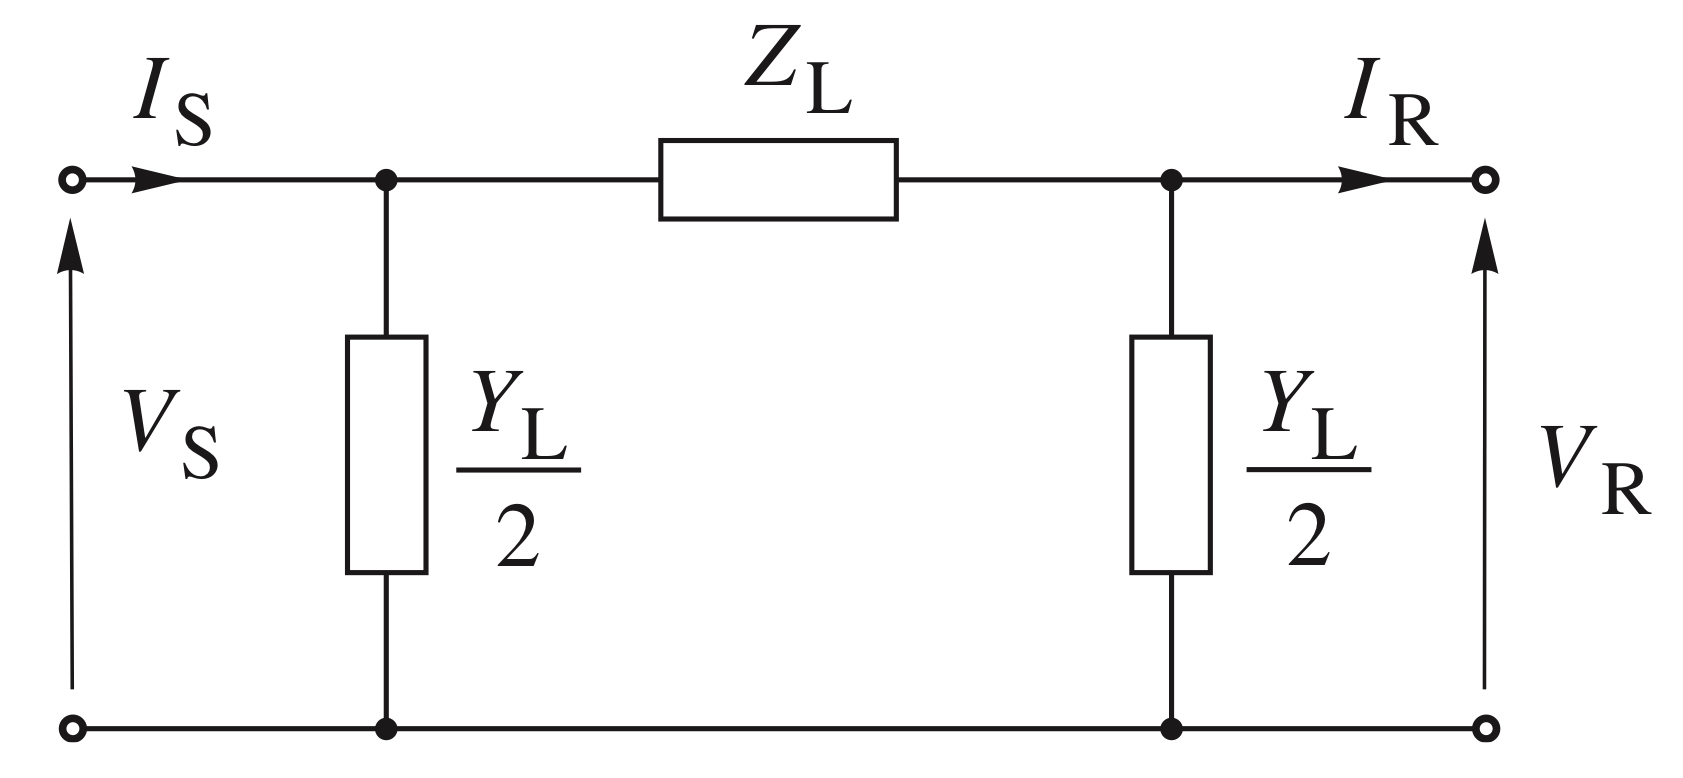
\includegraphics[width=0.9\textwidth]{Dissertation/images/pi_model.PNG}
    \caption{The $\pi$-equivalent of a power transmission line}
    \label{fig:pi_model}
\end{figure}

The receiving and sending physical quantities are linked via Kirchhoff law \cite{kirchhoff1847ueber}: 
$$
I_R = V_R \cdot Y_L/2 + (V_S - V_r) \cdot \frac{1}{Z_L}.
$$

\begin{comment}
The receiving voltages and current are linked between via long-line equation {\color{red} cite janusz, cite Power System Analysis: Grainger, John, Stevenson, William}:

\begin{equation}
    \begin{aligned}
        \begin{pmatrix}
            V_S  \\
            I_S 
        \end{pmatrix}
        =
        \begin{pmatrix}
            \cosh \gamma l      & Z_C \sinh \gamma l \\
            \sinh \gammal / Z_C & \cosh \gamma l
        \end{pmatrix}
        \begin{pmatrix}
            V_R  \\
            I_R 
        \end{pmatrix},
    \end{aligned}
    \label{eq:long-line}
\end{equation}
here $Z_C = \sqrt{z / y}$ is the characteristic, or surge, impedance of the power line and $\gamma = \sqrt{zy}$ is called the propagation constant.
\end{comment}

\subsection{Kirchhoff Current law and Admittance Matrix}

In the grid graph $\mathcal{G}$, a bus $b \in \mathbb{B}$ is connected to other buses $b' \in \textit{Adj}(b) = \{ b':~ \exists l = (b, b') ~\wedge~l' = (b', b) \in \mathcal{L} \}$.
The currents that flow through the lines are being Kirchhoff Current Law (KCL). 
Denote the current that flows into a bus $b\in \mathcal{B}$ as $I_b$, voltage at bus $b$ as $V_b$, shunt admittance of a line $(b, b')$ as $y^{sh}_{(b, b')}$ and line admittance as $y_{(b, b')}$ then:
\begin{equation}
    \begin{aligned}
        I_b &= \sum_{b' \in \textit{Adj}(b)} I_{(b,b')} = \\
            &= \sum_{b' \in \textit{Adj}(b)} \left( V_b y^{sh}_{(b, b')} + (V_b - V_{b'})y_{(b, b')} \right) = \\
            &= V_b\sum_{b' \in \textit{Adj}(b)} \left( y^{sh}_{(b, b')} + y_{(b, b')} \right) - \sum_{b' \in \textit{Adj}(b)} y_{(b,b')} V_{b'}.
    \end{aligned}
    \label{eq:KCL}
\end{equation}

To account for grid topology and KCL, all physical quantities that describe power line characteristics, i.e., impedance, are in a complex bus admittance matrix $Y \in \mathbb{C}^{|\mathcal{L}| \times |\mathcal{L}|}$. The matrix elements are organized as follows:
$$
Y_{ij} = 
\begin{cases}
\sum_{j \in \textit{Adj}(i)} y^{sh}_{ij} + y_{ij},& ~ i = j \\
-y_ij,& ~ i \neq j, ~ (i,j) \in \mathcal{L} \\
0, & ~ \textit{otherwise}.
\end{cases}
$$
The diagonal elements of this matrix are related to the self-admittance of each bus, while the other elements describe mutual admittance of connected buses.
Note that Equation \eqref{eq:KCL} can be rewritten using the elements of the admittance matrix $Y$ as follows:
\begin{equation}
    I_b =V_b Y_{bb} + \sum_{b' \in \textit{Adj}(b)} Y_{bb'}V_{b'} = \sum_{b' \in \mathcal{B}} Y_{bb'}V_{b'}.
    \label{eq:current_amd_V}
\end{equation}
Next, combining all bus current and voltages into corresponding vectors: $\boldsymbol{I} = (I_1, \dots, I_{|\mathcal{B}|})^\top, ~ \boldsymbol{V} = (V_1, \dots, V_{|\mathcal{B}|})^\top$ and obtain matrix form of Equation \eqref{eq:KCL}:

\begin{equation}
    \boldsymbol{I} = Y \boldsymbol{V}.
    \label{eq:KCL_matrix}
\end{equation}

Note that the complex-valued admittance matrix can be represented as $Y = G + i B$, where $G$ and $B$ are real-valued matrices.

\section{Power Flow Equations}
\label{sec:PFE}
The Power Flow Equations (PFEs) are describing the power injections -- the amount of electrical power that is put into or put out of a specific bus $i \in \mathcal{B}$. It allows to describe demand, genertion and the power that flows into a bus from the other sources in the power system.
It can be described in terms of voltage, phases and admittance matrix. 
The apparent power $S_i = \overline{V}_i \overline{I}_i^*$ can be written as follows, denote $\theta_{ij} = \phi_i - \phi_j$ - voltage phase angle difference between nodes $i$ and $j$ and using $i^{\textit{th}}$ equation in \eqref{eq:KCL_matrix}:
$$
S_i = \sum_{j=1}^{|\mathcal{B}|} |V_i||V_j| e^{j\theta_{ij}} (G_{ij} - j B_{ij}).
$$
Recalling that $S_i = P_i + iQ_i$ and expanding the exponent, one gets the real and imaginary parts: real and reactive power injections:
\begin{equation}
    \begin{aligned}
        P_i &= \sum_{i\neq j} |V_i||V_j| \left[ B_{ij} \sin(\theta_{ij}) + G_{ij} \cos(\theta_{ij}) \right] + V_i^2 G_{ii} \\ 
        Q_i &= \sum_{i\neq j} |V_i||V_j| \left[ G_{ij} \sin(\theta_{ij}) - B_{ij} \cos(\theta_{ij}) \right] - V_i^2 B_{ii}.
    \end{aligned}
    \label{eq:power_injections}
\end{equation}
% $$
% \overline{S}_i = (V_i \cos(\delta_i) + i V_i \sin(\delta_i)) \cdot  \left( (V_i \cos(\delta_i) + i V_i \sin(\delta_i)) \cdot (G_{ii} + i B_{ii}) + \sum_{i\neq j}  (G_{ii} + i B_{ii}) \cdot (V_i \cos(\delta_i) + i V_i \sin(\delta_i)) \right)
% $$

% Recall complex number representation current and voltage $V_i = |V_i| e^{i \delta_i}$, $Y_{ij} = |Y_{ij}| e^{j \theta_{ij}}$. Expanding apparent power $S_i$,  one obtains
% $$
% S_i = P_i + i Q_i = V_i I_i^* \underset{\eqref{eq:current_amd_V}}{=} |V_i|^2 |Y_{ii}| e^{-i \theta_{ii}} + V_i \sum_{j=1,j\neq i} |V_j| |Y_{ij}|e^{j(\delta_i - \delta_j - \theta_{ij})}.
% $$
% Next, one can separate real and imaginary parts
\chapter{Optimal Power Flow - OPF}
\label{chap:opf}

\section{Introduction}

Optimal Power Flow (OPF), proposed by Carpentier in 1962, is an optimization problem that seeks to find the cheapest generation set points over the set of generating units to satisfy the demand in a power system and meet technical limits that are given by Power Flow Equations, described in Chapter \ref{sec:PFE}, for a single time snapshot which is called steady-state OPF \cite{carpentier1962contribution}. This optimization problem is fundamental for a power system. Numerous modifications can help to obtain a range of results from intra-day generation schedule to the power system expansion plan \cite{bai2008semidefinite, molzahn2014investigation}.

The OPF is non-convex, due to the non-linearity of PFEs \eqref{eq:power_injections} and, generally, NP-hard \cite{lavaei2011zero}. Typically, instances of such class of problems are solved with iterative methods that require initial guess and guarantee local optimality \cite{molzahn2018towards}. Methods based on Linear Programming, Quadratic Programming, Newton's method, decomposition methods and interior-point based methods are well applied for the OPF. % cite for each method

This chapter is devoted to the OPF problem: its objective, variables, constraints, application-driven linear relaxation -- Direct Current OPF (DC-OPF) and dynamic OPF that models several temporarily interconnected timestamps of the system.

\section{Optimization problem}

A general constrained optimization problem problem is formulated as follows {\cite{red} BT, introduction to optimization}:

\begin{equation}
    \begin{aligned}
        \min            & J(x, u)    \\
        \texttt{s. t.}~ & g(x, u) = 0 \\
                        & h(x, u) \leq 0
    \end{aligned}
    \label{eq:constrained_opt}
\end{equation}
The vector $x \in \mathbb{R}^{n_x}$ is the vector of dependent variables, $u \in \mathbb{R}^{n_u}$ is the vector of decision variables, the cost function is scalar: $J: \mathbb{R}^{n_x + n_u} \to \mathbb{R}$. The equality and inequality constraints are given as the vector functions $g: \mathbb{R}^{n_x + n_u} \to \mathbb{R}^{m}$, $h: \mathbb{R}^{n_x + n_u} \to \mathbb{R}^{l}$. 

In OPF, the vector of independent variables consists of active power generation, voltage phases and magnitudes: $u = (p_g, v_m, \theta) \in \mathbb{R}^{|\mathcal{B}_G| + |\mathcal{B}| + |\mathcal{B}|}$. The objective function $J(x, u)$ is given by the total generation cost for OPF: $J(x, u) = J(p_g) = \textit{cost}(p_g)$, where $\textit{cost}: \mathbb{R}^{|\mathcal{B}_G|} \to \mathbb{R}$ is separable for each generator: 
\begin{equation}
\textit{cost} = \sum_{i \in \mathcal{B}_G} \textit{cost}_i (p_g^i).
\label{eq:objective_opf}
\end{equation}

\section{Constraints}

Constraints in OPF serve the purpose of ensuring meeting the demand, technical limits and transmission rules, induced by physical laws, are met within modeling. These constraints, as it was mentioned, classify into equality and inequality constraints and include power generation limits, power balance at buses, voltage limits, line limits and the reference bus constraints.

\subsection{Equality constraints}

Equality constraints include nodal power flow balance and PFEs \eqref{eq:power_injections}. For a bus $i \in \mathcal{B}$ let us denote $P_i^G, Q_i^G$ generated active and reactive power (0 if there is no generator at bus $i$) and $P_i^D, Q_i^D$ active and reactive power demand (0 if there is no load at bus $i$). Moreover, for a line $(i, j) \in \mathcal{L}$ let $P_{ij}, Q_{ij}$ be active and reactive line flows.  After a slight reformulation, these constraints are as follows: %{\color{red} find a reference preferably}
\begin{equation}
    \begin{aligned}
        P_i^G - P_i^D &= \sum_{j \in \textit{Adj}(i)} P_{ij}, ~i \in \mathcal{B} \\
        Q_i^G - Q_i^D &= \sum_{j \in \textit{Adj}(i)} Q_{ij}, ~i \in \mathcal{B} \\
    \end{aligned}
    \label{eq:nodal_flow}
\end{equation}
\begin{equation}
    \begin{aligned}
        P_{ij} &= V_i V_j \left[ G_{ij} \cos \theta_{ij} + B_{ij} \sin \theta_{ij} \right] - G_{ij} V_i^2, ~ij \in \mathcal{L} \\
        Q_{ij} &= V_i V_j \left[ G_{ij} \sin \theta_{ij} - B_{ij} \cos \theta_{ij} \right] + B_{ij} V_i^2, ~ij \in \mathcal{L} \\
    \end{aligned}
    \label{eq:line_flow}
\end{equation}

Assuming that reference bus is placed at bus $1 \in \mathcal{B}$, the slack bus constraint is
\begin{equation}
    \theta_1 = 0.
    \label{eq:slack_bus}
\end{equation}
\subsection{Inequality constraints}

Inequality constraints are induced by technical limits of lines (line ratings), generation technical limits and voltage limits for buses.

\paragraph{Generation limits}

The generator limits exist for ensuring that a generator is not requested to produce more power that it can and more power than minimal value to stay active. Let $\mathcal{G} \succ \mathcal{B}$ be the subset of buses that contain at least one generator. If there is multiple generators, the power generated from each one is summed and the results is the generation at bug $g \in \mathcal{G}$. Then limits are given, for $g \in \mathcal{G}$:
\begin{equation}
    \begin{aligned}
        P_g^{min} \leq &P_g^G \leq P_g^{max} \\
        Q_g^{min} \leq &Q_g^G \leq Q_g^{max} \\
        \label{eq:gen_lims}
    \end{aligned}
\end{equation}

\paragraph{Bus voltage limits}

To ensure safe operation of power grid, voltage is restricted by engineering limits. It is imposed on both magnitude and phase angle for each bus $i \in \mathcal{B}$:
\begin{equation}
    \begin{aligned}
        V_i^{min} \leq &V_i \leq V_i^{max} \\
        \theta_i^{min} \leq &\theta_i \leq \theta_i^{max} \\
        \label{eq:vol_lims}
    \end{aligned}
\end{equation}

\paragraph{Line rating}

Line rating, or line flow limits, are due to the wiring materials, components and length. Overhead lines that are subject to weather conditions have line rating that depend on the current weather condition and season \cite{fernandez2016review}. For a line $ij \in \mathcal{L}$ line rating are formulated as follows:
\begin{equation}
    P_{ij}^2 + Q_{ij}^2 \leq (S^{max}_{ij})^2.
    \label{eq:line_rating}
\end{equation}

\section{DC OPF Approximation}

In high voltage ($380$ kV, \cite{crucitti2005locating}) power grids, that are decribing a power system on inter-city country level, a common practice is to use Direct-Current OPF (DC-OPF) approximation. It does not assume direct current instead of alternating one. In fact, it has the following set of assumptions, recalling that $Y_{ij} = \frac{1}{R_{ij} + i X_{ij}}$ for a line $ij \in \mathcal{L}$:
\begin{enumerate}
    \item Voltage magnitudes are given in per units and approximately equal to one: $V_i \approx 1 ~ \forall i \in \mathcal{B}$
    \item Voltage phases does not differ much between buses: $\theta{ij} \approx 0, ~\forall ij \in \mathcal{L}$
    \item Line resistance is negligible: $R_{ij} ~ \forall ij \in \mathcal{L}$
\end{enumerate}

This set of assumption allows one to rewrite the AC-OPF constraints. Firstly, let us note that elements of the admittance matrix under the assumption 3) will be as follows, recall that $Y = G = i B$:
\begin{equation}
    Y_{ij} = \frac{1}{R_{ij} + i X_{ij}} \approx \frac{1}{iX_{ij}} \approx B_{ij}.
    \label{eq:admittance matrix approx}
\end{equation}
Next, assumption 2) yield the following approximation for trigonometric functions over phase difference, recalling Taylor's formula,%{\color{red} matan reference}
\begin{equation}
    \begin{aligned}
        \sin \theta_{ij} &= \theta_{ij} + o(\theta_{ij}) \underset{\theta_{ij} \to 0}{\to} \theta_{ij}    \\
        \cos \theta_{ij} &= 1 - \theta^2_{ij} / 2 + o(\theta_{ij}^2) \underset{\theta_{ij} \to 0}{\to} 1    \\
    \end{aligned}
    \label{eq:phase diff approx}
\end{equation}

Finally, combining \eqref{eq:admittance matrix approx}, \eqref{eq:phase diff approx} with 1) ($V_i V_j \approx 1$) and considering power flow lines \eqref{eq:line_flow} one obtains:
\begin{equation}
    \begin{aligned}
        P_{ij} &\approx B_{ij} \sin \theta_{ij} , ~ij \in \mathcal{L} \\
        Q_{ij} &\approx B_{ij} , ~ij \in \mathcal{L}. \\
    \end{aligned}
    \label{eq:line_flow_keked}
\end{equation}

Note that power flows are not constant only for active power and governed by the phase difference $\theta_{ij}$. Since all nonlinearities were held in the line flows, the resulting optimization problem DC-OPF is linear, provided linear cost function.

Let us summarize the DC-OPF below:

\begin{equation}
    \begin{aligned}
        \min_{P^G, \theta}  & \textit{cost}(P^G) \\
        \textit{s.t. }      & P^G - P^D = B\theta
                            & P_i^{min} \leq P_i^G \leq P_i^{max}, ~ i \in \mathcal{B} \\ 
                            & \sum_{i \in \mathcal{B}} P^G_i = \sum_{i \in \mathcal{B}} P^D_i \\
                            & |\theta_{ij}| \leq \bar{\theta}_{ij}, ~ ij \in \mathcal{L}
    \end{aligned}
    \label{eq:dc-opf}
\end{equation}

\section{Dynamic DC-OPF and Automated Generation Control}

Dynamic DC-OPF setup consider several system snapshots bound with temporal ramp-up and ramp-down constraints on generation \cite{lou2019multi, machowski2020power}. Such models allows for intra-day modeling of a system, taking into account load schedule and dynamics of renewable energy generation which can be treated as fluctuations.

Power systems fluctuations typically occur both on the generation and demand side and arise from the intermittency of renewable energy generation, unstable demand from the customers, and intra-day electricity trading. Often the distribution of such fluctuations can be recovered based on historical data \cite{roald2017chance,owen2019importance}. 
Below we assume that the fluctuations are Gaussian with the mean and covariance recoverable from historical data \cite{anvari2016short,roald2017chance}. 
The fluctuations are involved the power balance equation and typically managed through primary and secondary control \cite{machowski2020power}.
Let us index a system time snapshot as $t = 0, 1, \dots, T$ and denote fluctuations from generation that lead to imbalance as $(\xi_i^G)^t$ and $(\xi_i^D)^t$ -- from demand.
A common strategy to mitigate power imbalance is adopting linear Automatic Generation Control (AGC). The generation and demand fluctuate as $(P_i^G)^t + (\xi_i^G)^t$ at bus $i=1, \dots, n_g$ and $P^D_i + (\xi_i^D)^t$ at node $i=1,\dots, n_d$ respectively. As we assume that the initial generation is balanced, i.e., $\sum_{i=1}^{n_g} (P^G_i)^0 = \sum_{i=1}^{n_d} P_i^D$, the purpose of AGC is to balance the aggregated uncertainty term $\xi^t = \sum_{i=1}^{n_g}(\xi^G_i)^t-\sum_{i=1}^{n_d}(\xi^D_i)^t,$ where $\xi^t$ is distributed as the sum of all the nodes' uncertainties. For example, if the uncertainties are independent and identically distributed (i.i.d) Gaussians with mean $\mu = 0$ and some variance $\sigma^2$, then $\xi^t$ follows a Gaussian distribution $\mathcal{N}\left(0, (n_g+n_d) \cdot \sigma^2 \right)$. Following \cite{roald2017chance,baros2021examining,mezghani2020stochastic},
the AGC recourse brings the generation to a new setpoint $(P^G)^{t+1} = (P^G)^t + \alpha \xi^t$. In the latter the participation factors $\alpha \in \mathbb{R}^{n_g}$ satisfy $~\alpha \geq 0, ~ \boldsymbol{1}^\top \alpha = 1$. It is easy to check that if the system is initially balanced, then the new generation set-point also ensures a balanced system. The power mismatch at timestamp $t=1, \dots, T$ is given by:
$$
    1^\top p^t - 1^\top p_d - \xi^t = 1^\top p^{t-1} - 1^\top p_d + \xi^t - \xi^t = 0.
    \label{eq:power-balance-agc}
$$
i.e., this control strategy keeps the system balanced. 

In order to take into account limited rate of change of genration production, ramp-up and ramp-down constraints are induced and limit change of generation from one step to the next one by $\Delta_i \geq 0, ~ i \in \mathcal{B}$. 

Summing up, the dynamic DC-OPF formalizes as follows for a temporal snapshots $t = 0, \dots, T$:

\begin{equation}
    \begin{aligned}
        \min_{P^G, \theta}  & \sum_{t=1}^T\textit{cost}((P^G)^t) \\
        \textit{s.t. }      & (P^G)^t - (P^D)^t = B\theta^t\\
                            & P_i^{min} \leq (P_i^G)^t \leq P_i^{max}, ~ i \in \mathcal{B}, ~ t \in 0, \dots, T \\ 
                            & \sum_{i \in \mathcal{B}} (P^G_i)^t = \sum_{i \in \mathcal{B}} (P^D_i)^t, ~ t \in 0, \dots, T \\
                            & |\theta_{ij}^t| \leq \bar{\theta}_{ij}, ~ ij \in \mathcal{L}, ~ t \in 0, \dots, T \\
                            & |(P^G_i)^t - (P^G_i)^{t-1}| \leq \Delta_i.\\
    \end{aligned}
    \label{eq:dyn-dc-opf}
\end{equation}

\chapter{Power Grid Reliability Estimation via Adaptive Importance Sampling}
\label{chap:sampling}
This chapter based on publication on the author \fullcite{lukashevich2021importance}
\section{Introduction}
\label{sampling:introduction}

Carbon-free electricity generation is one of the most vital global challenges for the next decades. Because of their ecological and economic benefits, renewable energy sources, such as wind, hydro, and solar power generation, become more demanded, accessible, and widely used in modern power grids \cite{harjanne2019abandoning}. For instance, California's renewable portfolio standard currently requires 33\% of retail electricity sales to come from renewable resources, and will require 60\% by 2030, and 100\% by~2045~\cite{golden2003senate}.
However, renewable energy generation is highly volatile and brings significant uncertainty to power systems. This also gives rise to many challenges for power system operators trying to integrate renewables into power grids \cite{schmietendorf2017impact}. In particular, power systems operational policies and reliability assessment must be verified over various additional uncertainties, including increased variation in power generation and disturbances. 

Various algorithms have been developed so far for ensuring grid reliability. Some of them are based on machine learning, and utilize historical data about weather, renewables' generation, and grid operating parameters to estimate the risk of overload and influence of uncertainty due to weather changes~\cite{zhang2017data}. %,contingencyMLE}.
%3contingencymethods,
%,zhou2019wind
Requiring large datasets and high data collecting time to make an accurate prediction, machine learning methods become impractical for real-time operation if a large disturbance, contingency, or a sudden operational policy change precedes the reliability assessment. Another class of algorithms is based on analytical approximation of the overload probability~\cite{nemirovski2007convex}. In this approach, the risk of interest is upper-bounded by an integral of an appropriate function that admits analytical or numerical computation. However, even in the simplest case of linear reliability constraints and Gaussian fluctuations of renewables, existing approaches tend to overestimate the risk. Moreover, for a sufficiently rare event, the risk overestimation for these algorithms can be infinitely high~\cite{nemirovski2007convex} which compromises their practical~efficiency. 

Finally, algorithms based on sampling values of power generated by renewables and approximating the grid constraints overflow probability by its empirical counterpart often provide a valuable alternative for accessing the reliability posture of a power system. Monte-Carlo (MC), hybrid and Markov Chain MC have been earlier applied to risk-based reliability assessment of transmission power grids~\cite{su2005probabilistic,vittal2009steady,chen2008probabilistic}. 
%da1990probabilistic,
In~\cite{montecarlofeasibility}, the authors exploited Monte Carlo simulation for estimating overload probability and interpreted the risk by classifying it into low, medium and high risk operating points. Variations of the load-flow solution due to renewables fluctuation, nodal and line parameters uncertainty were considered in~\cite{su2005probabilistic}.  An inverse problem of wind turbine controls to meet reliability margins with high-probability is discussed in \cite{vittal2009steady}.  A comprehensive survey of sampling-based methods for power systems reliability assessment is given in~\cite{chen2008probabilistic}.
Unfortunately, these algorithms explore the space of fluctuations uniformly, which dramatically 
reduces their performance in understanding and evaluating the effect of a rare event such as a severe disturbance. 

Importance sampling is a valuable alternative to Monte-Carlo sampling, which allows adjusting distribution for generating more samples in the areas of interest, e.g., close to the reliability boundary. Pmvnorm~\cite{genz2020package} is one of the most efficient importance sampling algorithms in general, but its performance is often limited for rare events probability estimation~\cite{owen2019importance}, which is of the utmost importance to power systems study.  ALOE~\cite{owen2019importance}~is another efficient method designed especially for computing a rare event probability. However, it does not fully respect the geometry of reliability constraints. 
It thus requires a large number of samples to estimate the risk of constraint overflow, especially for large power grids and multi-line overloads. Finally, a convex optimization-based algorithm for adaptive importance sampling from exponential families was proposed in~\cite{ryu2014adaptive}. At each step, the algorithm adjusts the distribution parameters so that the sampler's variance is minimized. Unfortunately, the distribution of output power that leads to an overload is far from the exponential family,  limiting the algorithm's efficiency in power systems.

This chapter proposes an adaptive importance sampling method to efficiently estimate the risk of reliability constraints violation.
We present an importance sampling algorithm that uses physical information to generate a mixture of distributions to sample from and then uses convex optimization to iteratively adjust the weights of the mixture. Our algorithm substantially improves static weights assignment of ALOE~\cite{owen2019importance} when reliability constraints are highly correlated.
The approach allows to address the risk estimation problem in real-time even for large power grids with a small constraint overflow probability. We theoretically analyze the accuracy and complexity of our algorithm for the case of Gaussian power fluctuations from renewables; however, the technique is not limited to the Gaussian case. Finally, we evaluate the performance of our sampling methods over multiple real and synthetic test cases and compare it to the state-of-the-art. 

The chapter is organized as follows. 
In Section \ref{sampling:setup} we present the constraint overload probability estimation problem and introduce notation used in the chapter. We outline the importance sampling algorithm and present its theoretical analysis in Section \ref{sampling:prob}. Empirical study and comparison to the state-of-the-art are given in Section~\ref{sampling:emp}. In Section~\ref{sampling:conclusion} we conclude  with a brief summary and possible applications of our results. 

\section{Background and Problem Setup}\label{sampling:setup}

Being a popular load flow model, the higher-voltage direct current (DC) model remains simple for the analysis because of linear relations between power injections and phase angles. Let $G = (V, E)$ be a power grid graph with a set of buses~$V$, $|V| = n$ and a set of lines~$E$, $|E| = m$. Let $p \in \mathbb{R}^{n}$ and $\theta\in\mathbb{R}^{n}$ be vectors of power injections and phase angles respectively.  The power system is balanced, e.g., the sum of all power injections equals zero $\sum_{i \in V} p_i = 0$. To avoid ambiguity let $s$ be the slack bus and $\theta_s = 0.$ Let $B \in \mathbb{R}^{n \times n}$ be an admittance matrix of the system, $p = B\theta$. The components $B_{ij}$ are such that $B_{ij} \neq 0$ if there is a line between buses $i$ and $j$ and  for any node $B_{ii} = - \sum_{j\neq i} B_{ij}$, e.g., $B$ is a Laplacian matrix.  Let $B^{\dagger}$ be the pseudo-inverse of $B$, $\theta = B^{\dagger} p$. The DC power flow equations, generation and reliability constraints are 
\begin{subequations}
\label{eq:DC-PF}
    \begin{equation}
        p = B \theta
        \label{eq:DC-PF-a}
    \end{equation}
    \begin{equation}
        \underline{p}_i \leq p_i \leq \overline{p}_i
        \label{eq:DC-PF-b}, i \in V \text{ and } |\theta_i - \theta_j| \leq \bar{\theta}_{ij}, \; (i,j)\in E
    \end{equation}
    %\begin{equation}
    %    |\theta_i - \theta_j| \leq \bar{\theta}_{ij}, \; (i,j)\in E
    %    \label{eq:DC-PF-c}
    %\end{equation}
\end{subequations}
Reliability constraints~\eqref{eq:DC-PF-b} %, \eqref{eq:DC-PF-c} 
define a polytope $P$ in the space of power injections, $P = \{p: W p \le b\}$, so that the reliability constraints are violated if and only if power injections $p \not\in P.$ 

To derive an explicit expression of matrix $W$ we consider the incidence matrix $A$, such that for any buses $i$ and $j$ with $i<j$ connected by an edge $k$, $A_{ki} = 1$, $A_{kj} = -1$ and all other elements in row $k$ are equal to zero. Then the phase angle constraints are $AB^{\dagger}p \le \bar\theta$, $-AB^{\dagger}p \le \bar\theta$. 
%
Finally, as the slack bus balances the system, $p_s = -\sum_{i\neq s} p_i$ let $C \in \mathbb{R}^{n\times n}$ be a symmetric matrix such that for any non-slack buses $i$ and $j$, and the slack bus $s$, $C_{ii} = 1$, $C_{ij} = 0$, $C_{ss}=0$, and $C_{is} = -1$. In other words, $C p$ is a vector of grid power injections expressed in terms of non-slack injections only, since the slack bus power injection is fully determined by the other ones. 


Finally, from Eqs.~\eqref{eq:DC-PF} the following system of inequalities defines the reliability polytope, $P = \{p: Wp \le b\}$,
\begin{equation}
(AB^\dagger C, - A B^\dagger C, C, -C)^\top p \le (\bar\theta, \bar\theta, \overline{p}, \underline{p})^\top, 
\label{eq:feasibility_ineqs}
\end{equation}
with $W = (AB^\dagger C, - A B^\dagger C, C, -C)^\top$, $b = (\bar\theta, \bar\theta, \overline{p}, \underline{p})^\top$\!\!\!. Let $J = 2m + 2n$ be a number of constraints, e.g., rows in matrix $W$, then the reliability polytope $P$ is $\bigl\{p\!:\! \bigcap_{i=1}^J p^\top\!\!\omega^i \le b_i\bigr\}$. 

Stochastic uncertainty in renewable generation and power consumption imposes a question of power grid reliability, e.g., estimating a probability that at least one of the reliability constraints is violated. Namely, we consider Gaussian fluctuations of power injections $p$ with known mean $\mu$ and covariance $\Sigma$ and aim at computing a constraint violation probability $\Pi$:
\begin{align}\label{eq:prob}
    \Pi = \mathbb{P}(p\not\in P) = \int_{\mathbb{R}^n} \upsilon(p) 1[p\not\in P] d p, \; p\sim \mathcal{N}(\mu, \Sigma), 
\end{align}
where $\mathbb{P}$ is a probability taken w.r.t. the normal pdf $\upsilon(p)$ of $p$. 

Notice, that the probability $\Pi$ does not have an analytic expression, is computationally intractable, and even hard to approximate~\cite{owen2019importance,ryu2014adaptive,cappe2008adaptive, khachiyan1989problem}. 
In practice, a union bound is often used to upper bound $\Pi$. Let $\Pi_i$ be a probability of a single event, e.g., $p^\top\omega^i > b_i$. It has an explicit expression for the Gaussian distribution, and by union bound inequality
$\sum_{i\le J}\Pi_i \ge \Pi \ge \max_{i\le J} \Pi_i$; however, the bounds are loose when dealing with correlated violations which is often the case for power systems. 

To refine the overload estimate and take into account simultaneous violation of multiple constraints, we propose an importance sampling procedure that allows to count the average number of constraints $N$ violated at the same time and, thus, improve the overload probability estimation to $\Pi/N$ instead of $\Pi$. It is meaningful for large power grids where multiple events are likely to happen synchronously.

Table~\ref{tab:notation} summarizes chapter's notation. We use lower indices for elements of vectors and matrices, lower-case letters for probability density functions (pdfs), and upper-case letters for cumulative distribution functions (cdfs). When it does not lead to confusion, we use $\mathbb{P}$, $\mathbb{E}$, $\mathbb{V}$ to denote  probability, expectation, and variance without explicitly mentioning a distribution. 

\begin{table}[t]
    \centering
    \captionsetup{justification=centering}
    \caption{Chapter notation.}
    \begin{tabular}{l|l|l|l}
        $E$ & set of lines, $|E| = m$ & $\upsilon(p)$ & nominal distribution pdf\\
        $V$ & set of buses, $|V| = n$ & $\upsilon_D$ & parametric distribution pdf\\
        $B$ & $n\times n$ admittance matrix& $x$ & mixture distribution para- \\
        $p_i$ & power injection & & meters, $x\in X \subseteq \mathbb{R}^J$\\
        $\underline{p}_i$ & lower generation limit & 
        $D_i$& $p\!\sim\!\mathcal{N}(\!\mu, \!\Sigma)$ s.t. $p^\top\! \omega^i \!> \!b_i$\hspace{-5mm}\\
        $\overline{p}_i$ & upper generation limit & $N$ & number of samples\\
        $\theta_i$ & phase angle & $\mathbb{P}$, $\mathbb{E}$ & probability, expectation\\
        $\theta_{ij}$ & phase angle difference%, $\theta_i - \theta_j$
        &$\mathbb{V}$, $\kl$ & Variance, KL-divergence\\
        $\bar\theta_{ij}$ & angle difference limits & ${\mathcal{N}}\!(\mu, \!\Sigma)\hspace{-5mm}$ &  Gaussian distribution with\\
        $I_n$ & $n\times n$ identity matrix & & mean $\mu$ and covariance $\Sigma$\\
        $J$ & number of constraints & $\Phi$ & ${\mathcal{N}}(0,1)$ distribution cdf\\ 
        ${P}$ & reliability set, $p\!:\! W p \!\le\! b\!\!\!\!$ & $U(0,1)$ & uniform $(0,1)$ distribution\\
        $\omega^i$ & rows of matrix $W$, $i\le J$ & $\Pi$ & overflow probability, $\!p\not\in\! P$
    \end{tabular}
    \label{tab:notation}
    \vspace{-4mm}
\end{table}


\section{Overload Probability Estimation}\label{sampling:prob}

\subsection{A Single Constraint Case}
We start with estimating the probability of fluctuating power injections to cause an overload of an individual constraint, e.g., $\Pi_i = \mathbb{P}(p^\top \omega^i \ge b_i)$ for some $i$, $1\le i \le J$. In the case of a Gaussian distribution, $p\sim \mathcal{N}(\mu,\Sigma)$ there is a closed form expression for it:
% \begin{align*}
% \Pi_i & = \mathbb{P}_{p\sim \mathcal{N}(\mu, \Sigma)}(p^\top \omega^i \ge b_i)  = \mathbb{P}((p - \mu)^\top \omega^i \ge b_i - \mu^\top \omega^i)\\
% & = \mathbb{P}_{{\tilde p}\sim \mathcal{N}(0, I_n)} \left((\Sigma^{1/2}\omega^i)^\top {\tilde p} \ge b_i - \mu^\top \omega^i\right) \\
% & = \mathbb{P}_{{\tilde p}\sim \mathcal{N}(0, I_n)} \left( {\tilde p}^\top {\bar\omega}_i \ge (b_i - \mu^\top \omega^i)/\|\Sigma^{1/2}\omega^i\|_2\right)  \\
% & = \Phi((b_i - \mu^\top \omega^i)/\|\Sigma^{1/2}\omega^i\|_2), 
% \end{align*}
$%$\begin{align*}
\Pi_i  = \mathbb{P}_{p\sim \mathcal{N}(\mu, \Sigma)}(p^\top \omega^i \ge b_i) %\\
%& = \mathbb{P}_{{\tilde p}\sim \mathcal{N}(0, I_n)} \left( {\tilde p}^\top {\bar\omega}_i \ge (b_i - \mu^\top \omega^i)/\|\Sigma^{1/2}\omega^i\|_2\right)  \\
 = \Phi((b_i - \mu^\top \omega^i)/\|\Sigma^{1/2}\omega^i\|_2), 
$%\end{align*}
where $\Phi$ is the standard Gaussian distribution cdf, ${\tilde p} = \Sigma^{-1/2}(p-\mu)$, ${\bar\omega}_i = (\Sigma^{1/2}\omega^i)^\top/\|\Sigma^{1/2}\omega^i\|_2$, and $1\le i \le J$. $\Pi_i$ are the probabilities of $p^\top \omega^i \ge b_i$, so that 
$
    \Pi = \mathbb{P}(\exists i: p^\top \omega^i \ge b_i) \le \sum_{i\le J}\mathbb{P}(p^\top \omega^i \ge b_i) = \sum_{i\le J} \Pi_i.
$

Algorithm~\ref{alg:sample1d} is an instance of the inverse transorm method \cite{l2009monte} which allows to sample $p \sim \mathcal{N}(\mu, \Sigma)$ s.t. $p^\top \omega^i > b_i$. We refer this distribution as $D_i$, and its pdf is $\upsilon(p)/\Pi_i$ if $p^\top \omega^i > b_i$ and $0$ otherwise. Notice, that sample $p \sim \mathcal{N}(\mu, \Sigma)$ can be obtained with the plain MC from $\mathcal{N}(\mu, \Sigma)$, but it requires on average $1/\Pi_i$ trials instead of just one for Algorithm~\ref{alg:sample1d}.

\begin{algorithm}[H]
    \SetKwInOut{Input}{input}
    \SetKwInOut{Output}{output}
    \caption{Sampling $p\sim \mathcal{N}(\mu,\Sigma)$ s.t. $p^\top \omega^i \geq b_i$}
    \label{alg:sample1d}
    \Input{Mean $\mu$, covariance $\Sigma$, and a constraint $p^\top \omega^i \le b_i$} 
    \Output{$p\sim\mathcal{N}(\mu,\Sigma)$ s.t. $p^\top \omega^i \ge b_i$}
    Sample $z \sim \mathcal{N}(0, I_n)$ and $u \sim U(0,1)$\;
    Compute $y = \Phi^{-1}(\Phi(\tau) + u(1 - \Phi(\tau)))$\;
    Set $\phi = \bar\phi y + (I_n - \bar\phi\phi^\top) z$, with $\bar\phi = \Sigma^{1/2} \omega^i / \|\Sigma^{1/2} \omega^i\|_2$\!\! \;
    \Return $p = \Sigma^{1/2} (\phi+\mu)$
\end{algorithm}

 
 \subsection{Multiple Constraints Case}
 
The case of multiple constraints is more involved. Indeed, there is no analytical formula for an overload probability and, moreover, its exact computation is intractable~\cite{khachiyan1989problem}. 
%The plain 
Monte-Carlo sampling, $p\sim \mathcal{N}(\mu, \Sigma)$ is inefficient in estimating the constraint overload probability, especially if it is small. Indeed, it requires on average $O(1/\Pi)$ samples to get at least one of the outside the reliability polytope, $p\not\in P$. 

The importance sampling idea is to change the distribution one samples from and assign a weight to each sample to account for the~change: 
\begin{align*}
    \Pi  = \mathbb{P}(p\not\in P) & = \int_{\mathbb{R}^n} f(p) \upsilon(p) dp = \!\int_{\mathbb{R}^n}\!\! \frac{f(p)\upsilon(p)}{\upsilon_D(p,x)}\upsilon_D(p,x) dp%\\
    %& \approx \frac{1}{N}\sum_{i=1}^N \frac{f(p^i)\upsilon(p^i)}{\upsilon_D(p^i,x)}, p^i \sim %\upsilon_D(p,x),
\end{align*}
where we refer to $\upsilon(p)$ as \emph{nominal} distribution, and $\upsilon_D(p,x)$ as \emph{synthetic} distribution with parameter $x$,  $f(p) = 1[p\not\in P]$. 

A natural extension of importance sampling with a single linear constraint to the case of multiple linear constraints is to sample from a mixture distribution: 
%\begin{align}\label{eq:mix}
    $D = \sum_{i \le J} x_i D_i, \text{ with } \sum_{i\le J} x_i = 1, x_i \ge 0, \; 1\le i \le J,$
%\end{align}
where $D_i$ is $\mathcal{N}(\mu,\Sigma)$ conditioned on $p^\top\omega^i > \!b_i$. 
%
The sampling algorithm consists of two steps. First, we choose a distribution $D_i$ with probability $x_i$. Second, we sample $p \sim D_i$, i.e. $p\sim \mathcal{N}(\mu,\Sigma)$ given $p^\top\omega^i>b_i$, according to Algorithm~\ref{alg:sample1d}.
%
Probability density function $\upsilon_D(p, x)$ of $D$ is given by
    $\upsilon_D(p, x) = \sum\limits_{i\le J} x_i \upsilon_i(p) 1[p^\top \omega^i > b_i]/\Pi_i$,
    %
    %\begin{cases}
    %0, & \!\!p \in P,\\
    %\sum_{i\le J} x_i \upsilon_i(p) 1[p^\top \omega^i > b_i], & \!\!p\not\in P,
    %\end{cases}
%\end{align*}
where $1[\cdot]$ is a binary indicator, and 
$%\begin{align*}
    \upsilon_i(p) = \upsilon(p) 1[p^\top\omega^i > b_i]/\Phi((b_i - \mu^\top\omega^i)/\|\Sigma^{1/2}\omega^i\|_2).
$%\end{align*}

In contrast to the classical Monte-Carlo, which explores the uncertainty space uniformly according to the nominal distribution, importance sampling from parametric distribution $\upsilon_D(p,x)$ yields samples only from the area of interest, i.e., $p\not\in P$. 
More specifically, Monte-Carlo generates many samples from the true distribution of power injections to estimate overflow probability, while the proposed approach only samples power injections that lead to an overload and adjusts their weights.
Figure \ref{fig:00} illustrates the difference. 

\begin{figure}
    \centering
    % \vspace{-3mm}
    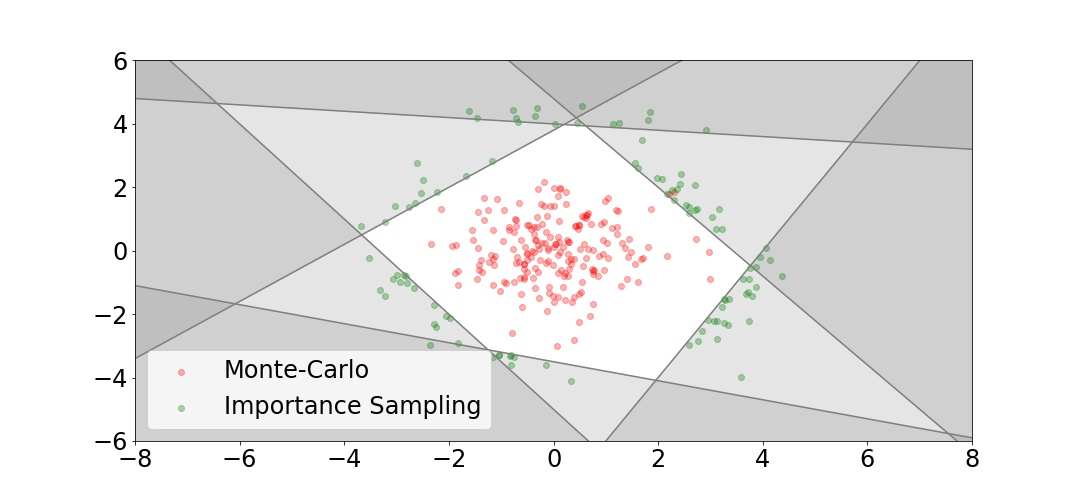
\includegraphics[width=.95\textwidth]{Dissertation/images/sampling/conditioned_vs_MC.jpg}
    % \vspace{-5mm}
    \caption{White area stands for generations that do not exceed operating limits. A set of generations leading to at least one constraint violation is in grey. Two or more reliability constraints are not satisfied in dark grey area. Samples from a nominal distribution and the constructed mixture marked in red and green resp. 
    }
    \label{fig:00}
    % \vspace{-5mm}
\end{figure}

Having a distribution mixture $\{D_i\}_{i=1}^J$we are looking for the weights $\{x_i\}_{i=1}^J$ to approximate a distribution $D$, $p \sim \mathcal{N}(\mu, \Sigma)$ s.t. $p\not\in P$, in the optimal way. Note that, any positive $\{x_i\}_{i=1}^J$ weights lead to an unbiased estimate 
\begin{align}\label{eq:aloe}
    {\hat \Pi} = N^{-1}\sum_{i=1}^N \upsilon(p^i)/\upsilon_D(p^i, x^i), \quad p^i \sim D^{x^i}
\end{align}
of the probability $\Pi$. Here $x^i$ is the vector of mixture weights for $i^{\textup{th}}$ sample. Indeed, by linearity of the  expectation $\mathbb{E}_{\upsilon_D(p,x)} \hat \Pi = \frac{1}{n}\sum_{i\le n} \int \frac{\upsilon(p^i)1[p^i\not\in P]}{\upsilon_D^{-1}(p^i, x)}\upsilon_D(p^i, x) dp = \Pi$. 

Despite being unbiased for any $x$ with positive components, variance of the  estimate~\eqref{eq:aloe} highly depends on the choice of $x$.
In \cite{owen2019importance} the authors suggested to take $x_i \propto \Pi_i$. 
While it leads to a consistent estimate, the estimator's variance is still high, especially when violation of multiple constraints is likely to happen in the system \cite{owen2019importance}. In practice, it leads to high sample complexity of the estimator which compromises its real time application. In the next subsection, we significantly improve the sampler's efficiency by using convex optimization to find the optimal combination of the mixture distribution weights $x$. 

\subsection{Convexity of Importance Sampling Variance}

We will measure the effectiveness of our estimator by its mean squared error, which is equal to the variance since the estimator is unbiased.
The importance sampler variance is 
\begin{align*}
    \bV_{\upsilon_D(p, x)}\left(\frac{\upsilon(p) f(p)}{\upsilon_D(p, x)}\right) %\int_{p\in\mathbb{R}^n}\!\! \left(\frac{f(p)\upsilon(p)}{\upsilon_D(p, x)} - \Pi\right)^2 %\!\!\upsilon_D(p, x) d p \\
     = \int_{p\in\mathbb{R}^n}\!\! \frac{f^2(p)\upsilon^2(p)}{\upsilon_D(p, x)} d p - \Pi^2 =: V(x), 
\end{align*}
where $f(p) = 1[p\not\in P]$. 

The optimal synthetic distribution can be chosen to minimize the variance, $\upsilon_*(p) = f(p)\upsilon(p)/\Pi$, and thus provide a better approximation to the integral. Notice, that for $\upsilon_D = \upsilon_*$ the variance $V(x) = 0$ and attains its minimum.  However, if $\upsilon_*(p)$ does not belong to the parametric family $\{\upsilon_D(p,x)\}_x$, we are looking for the best approximation of $\upsilon_*(p)$ within it, i.e. a minimum possible value of $V(x)$. 

Figure~\ref{fig:fscheme} illustrates our approach. Starting from an initial weight assignment, $x_i^1 \propto \Pi_i$, at each iteration $N$ of the algorithm we sample $p^k \sim \upsilon_D(\cdot, x^k)$ and compute $x^{k+1}$ to minimize the variance of the estimate. We also update an empirical estimate to the probability 
\begin{align}
    \hat \Pi = \frac{1}{k}\sum_{t=1}^k \frac{\upsilon(p^t) f(p^t)}{\upsilon_D(p^t, x^t)}, \; p^t \sim \upsilon_D(\cdot, x^t), t\le k \label{eq:emp}
\end{align}
and update parameters $x$ based on the value of $V(x^N)$ and its gradient. Before discussing the update strategy for the parameters $x$, we  outline some important properties of the variance $V(x)$ and empirical estimate~\eqref{eq:emp}. 

\begin{figure}
    \centering
    \begin{tikzpicture}[scale=0.7, node distance={15mm}, thick, main/.style = {draw, scale=.9}] 
    \node[main] (a)  {Define distributions $D_i$, \par $p\sim \mathcal{N}(\mu, \Sigma)$ s.t. $p^\top \omega^i\ge b^i$}; 
    \node[main] (b) [below = 4 mm of a] {Choose weights $x$ of the mixture, $p\sim\sum_{i\le J}x_i D_i$}; 
    \node[main] (c) [below = 2 mm of b] {Sample $p \sim \Psi(p, x) = \sum_{i\le J }x_i D_i$}; 
    \node (x) [below = 3 mm of c]{};
    \node[main] (d) [left =  6 mm of x] {Update weights vector $x$};
    \node[main] (e) [right = 4 mm of x] {Update overload estimate $\Pi^N$}; 
    \draw[->] (a) -- (b) node[midway, right] { {\footnotesize set $x_i\propto \Pi_i$}};
    \draw[->] (b) -- (c);
    \draw[<-] (-4.0,-1.95) -- (-4.0,-2.75);
    %\draw[-] (-4.0,-4.9) -- (-4.0,-1.5);
    \draw[->] (c) -- (d); 
    \draw[->] (c) -- (e);
    %\draw[->] (d) -- (e);
    \end{tikzpicture} 
    \caption{Scheme of the proposed algorithm. First, we initialize distributions $D_i$ based on a given set of constraints. Second, we initialize the weights of a mixture distribution to sample  $x_i\propto \Pi_i$. Then, with each new sample from $\sum_{i\le J} x_i D_i$ we update the weight vector $x$ and a overload estimate $\Pi_n$. See Eq.~\eqref{eq:md-upd} for details.}
    \label{fig:fscheme}
    % \vspace{-4mm}
\end{figure}

Theorem~\ref{thm:var-convexity} implies convexity of the variance minimization %problem 
\begin{align}
    \min_x \; & V(x), \; 
    \text{s.t. } x_1 + \dots + x_J = 1, x_i \ge 0, 1\!\le\! i \!\le\! J\label{eq:var-min}
\end{align}
in $x$ for the mixture distribution $\upsilon_D(p,x) = \sum_{i=1}^J x_i \upsilon_i(p)$. %To improve numerical stability one may also add constraints $x_i \ge \varepsilon > 0$ that guarantee that the variance is bounded.

\begin{theorem}\label{thm:var-convexity}
Problem~\eqref{eq:var-min} is convex in $x$, and for $x > 0$
\begin{align*}
    \nabla V(x) = \int_{\mathbb{R}^n} - f^2 (p)\upsilon^2(p)\upsilon_D^{-2}(p,x) (\upsilon_1(p), \dots, \upsilon_J(p))^\top dp.
\end{align*} 
\end{theorem}
\begin{proof}
The sub-integral expression, $f^2(p)\upsilon^2(p)/\upsilon_D(p,x)$, is convex for any $x > 0$ as
\begin{align*}
    \nabla^2_x \left[f^2(p)\upsilon^2(p)/\upsilon_D(p,x)\right] = 2f^2(p)\upsilon^2(p)/\upsilon^3_D(p,x) h h^\top \!\succeq\! 0,
\end{align*}
where $h = (\upsilon_1(p), \dots, \upsilon_J(p))^\top = \nabla_x \upsilon_D(p,x)$. 
The latter implies the integral's convexity. %Indeed, the Hessian of the sub-integral expression is non-negative for any $x$ 
Finally, by the dominated convergence theorem as $\mathbb{E}_{p \sim \upsilon_D(\cdot,x)} \nabla_x\left[f^2(p)\upsilon^2(p)/\upsilon_D(p,x)\right]$ is finite for $x>0$, one can exchange the order of differentiation and integration and 
%\begin{align*}
$\nabla V(x) = -\int \frac{f^2 (p)\upsilon^2(p)}{\upsilon_D^2(p,x)} h^\top dp.$
 %\int_{\mathbb{R^n}}\nabla_x \frac{f^2(p)\upsilon^2(p)}{\upsilon_D(p,x)} dp 
 %
%\mathbb{E}_{p \sim \upsilon_D(\cdot,x)} & 
%\left[- \frac{f^2(p)\upsilon^2(p)}{\upsilon_D^2(p,x)}h^\top\right] = \
%\mathbb{E}_{p \sim \upsilon_D(\cdot,x)} % z\nabla_x\!\!\left[\frac{f^2(p)\upsilon^2(p)}{\upsilon_D(p,x)}\right] \\
%& = 
%    \nabla_x \mathbb{E}_{p \sim \upsilon_D(\cdot,x)}  %\left[\frac{f^2(p)\upsilon^2(p)}{\upsilon_D(p,x)}\right] = \nabla V(x).%,
%\end{align*}
%which concludes the proof of the theorem. 
\end{proof}


\begin{theorem}\label{thm:unbias}
$\hat \Pi$ is an unbiased estimate of $\Pi$ if for all $k$, $1\le k \le N$, $x_k > 0$ and $x_k$ is independent of $x^j$ and $p^j$ for~$N\ge j > k\ge 1$.
\end{theorem}
\begin{proof} 
By the law of total expectation for $f(p) \!=\! 1[p\!\not\in\! P]$
\begin{align*}
    \mathbb{E}\, {\hat\Pi} & = \frac{1}{n}\sum_{k=1}^n  \mathbb{E}\biggl[\mathbb{E}_{p^k\sim\upsilon_D(p, x^k)} \biggl[ \frac{\upsilon(p^k) f(p^k)}{\upsilon_D(p^k,x^k)}\big| x^k\biggr]\biggr] = \Pi, %\sum_{i=1}^n \frac{\Pi}{n}= \Pi,
\end{align*}
as $\mathbb{E}_{p^k} \bigl[ \frac{\upsilon(p^k)f(p^k)}{\upsilon_D(p^k,x^k)}\big| x^k\bigr] = \Pi$. %\!=\! \int \frac{\upsilon(p^k)1[p^k \not\in P]}{\upsilon_D(p^k,x^k)}\upsilon_D(p^k,x^k) dp^k
\end{proof}

According to Theorem~\ref{thm:unbias}, the importance sampling estimate is unbiased. Theorem \ref{thm:var} bounds the variance of $\hat\Pi$. 

\begin{theorem}\label{thm:var}
Variance of $\hat\Pi$ equals $N^{-2}\sum_{k=1}^N V(x^k)$ if for all $k$ and $j,$ $1\le k < j \le N$, $x_k > 0$ and $x_k$ is independent of $x^j$ and~$p^j$.
\end{theorem}
\begin{proof} For $f(p) = 1[p\not\in P]$, $\mathbb{V} (\hat\Pi)\!=\! \mathbb{E}(\hat\Pi - \Pi)^2$ one has 
\begin{align*}
    &\mathbb{V}(\hat\Pi) = \frac{1}{N^2} \sum_{k=1}^N \mathbb{E}\biggl( \frac{\upsilon(p^k)f(p^k)}{\upsilon_D(p^k, x^i)} - \Pi\biggr)^2
    \\ & 
    \; + \frac{2}{N^2}\sum_{k < j} \mathbb{E} \biggl(\frac{\upsilon(p^k)f(p^k)}{\upsilon_D(p^k, x^k)} - \Pi\biggr)\biggl(\frac{\upsilon(p^j)f(p^j)}{\upsilon_D(p^j, x^j)} - \Pi\biggr)\\
    & = \frac{1}{N^2}\sum_{k=1}^N \mathbb{E}\biggl[\mathbb{E}\biggl[\biggl(\frac{\upsilon(p^k)f(p^k)}{\upsilon_D(p^k,x^k)} - \Pi\biggr)\big| x^k\biggr]\biggr] \\
        & + \frac{2}{N^2}\sum_{k < j} \mathbb{E}\mathbb{E}\biggl[ \biggl(\frac{\upsilon(p^k)f(p^k)}{\upsilon_D(p^k, x^k)} - \Pi\biggr)\!\!\biggl(\frac{\upsilon(p^j)f(p^j)}{\upsilon_D(p^j, x^j)} - \Pi\biggr)\big|x^k\biggr],
\end{align*}
where the latter is equal to $N^{-2}\sum_{k=1}^N V(x^k)$.
\end{proof}

In the next section, we present a numerical method that guarantees convergence of $V(x^N)$ to the optimal value $V^*$ with an additive error~$O(1/\sqrt{N})$.

\subsection{Numerical Method}\label{sampling:nm}

In this section we focus on efficient numerical methods for minimizing variance which, therefore, accelerate convergence of the importance sampling procedure. The mirror descent \cite{nemirovski2009robust} is known for its efficiency for simplex-constrained minimization problems. Its particular advantage compared to the stochastic gradient descent~\cite{ryu2014adaptive} and other optimization algorithms is only a logarithmic dependence on the problem dimension. 
%
The mirror descent update for solving Prob.~\eqref{eq:var-min}
%\begin{align}\label{eq:md-problem}
%    \min_{x \ge 0, \sum_{i\le J} x_i = 1} V(x),
%\end{align}
is an iterative modification of a point $x^k$ according to
\begin{align}\label{eq:md-upd}
    \!\!x^{k+1} = \argmin\limits_{x\in S}\left\{\eta^k \nabla V(x^k)^\top (x - x^k) + D_\omega(x, x^k)\right\}\!\!,
\end{align}
where $S =\{x \ge 0,x_1+\dots+ x_J = 1\}$, a step-size $\eta^k \!>\! 0$, 
$D_\omega(x, x^k)$ is the Bregman divergence defined for any strongly convex and smooth (distance-generating) function~$\omega$~as
$
    D_\omega(x, x^k) = \omega(x) - \{\omega(x^k) + \nabla \omega(x^k)^\top (x^k - x)\}.
$
So as the distance generating function is strongly convex and smooth in $x,$ so is the Bregman divergence. When $\omega(x) = \|x\|_2^2/2,$ mirror descent step is the same as in the gradient descent method, $x^{k+1} = x_k - \eta^k \nabla V(x^k)$. However, the negative entropy, $\omega(x) = -\sum_{i=1}^n x_i \log x_i$, is known to be the optimal choice for simplex constrained optimization. For $k\ge 1$ and $1\le i \le J$, solving~Eq.~\eqref{eq:md-upd} in $x$ leads to an update 
\begin{align}
\label{eq:_upd}x^{k+1}_i = x^k_i \frac{\exp(-\eta^k(\nabla V(x^k))_i)}{\sum_{j=1}^J x^k_j \exp(-\eta^k(\nabla V(x^k))_j)}, \eta^k > 0.
\end{align}

Finally, upon minimizing stochastic objective $V(x),$ the expectation of the gradient is inaccessible, so one substitutes $\nabla V(x)$ with a stochastic gradient that comes from the uncertainty realization~$p$,
$g(x, p) =  - f^2 (p)\upsilon^2(p)\upsilon_D^{-3}(p,x) h^\top, \; \mathbb{E}_{p\sim \upsilon_D}g(x, p) = \nabla V(x),$
and $h = (\upsilon_1(p), \dots, \upsilon_k(p))$. Finally 
$
    \upsilon_D(p,x)/\upsilon(p) = \sum_{i\le J} x_i 1[p^\top \omega^i \ge b_i] / \Pi_i,
$
and $f(p) = 1 $ for any $p\sim\upsilon_D$; 
$g_i (x^k, p) \!=\! \Pi_i^{-1} 1[p^\top \omega^i \!>\! b_i]/(\sum_{j\le J} x_j^k 1[p^\top \omega^j \!>\! b_j])^3$, $i\!\le\!J$. %/ \Pi_j\right)^3})$, $1\le i \le J$.

%\begin{align}\label{eq:_upd}
%    x^{k+1}_i = \frac{x^k_i \exp\left(\frac{\eta^k \upsilon(p) 1[p^\top \omega^i > b_i]}{\sum_{j\le J} x_j^k 1[p^\top \omega_j \ge b_j]}\right)}{\sum_{j=1}^J x_j^k \exp\left(\frac{\eta^k \upsilon(p) 1[p^\top \omega_j > b_j]}{\sum_{i\le J} x_i 1[p^\top \omega^i \ge b_i]}\right)}, 1\le i \le J.
%\end{align}
%{\color{blue}
%\begin{align}\label{eq:_upd}
%    x^{k+1}_i = \frac{x^k_i \exp\left(\frac{\eta^k \upsilon(p) 1[p^\top \omega^i > b_i] / \Pi_i}{\left( %\sum_{j\le J} x_j^k 1[p^\top \omega_j \ge b_j] / \Pi_j\right)^3}\right)}{\sum_{l \leq J}x^k_l %\exp\left(\frac{\eta^k \upsilon(p) 1[p^\top \omega_l > b_l] / \Pi_l}{\left( \sum_{j\le J} x_j^k 1[p^\top %\omega_j \ge b_j] / \Pi_j\right)^3}\right)}, 1\le i \le J.
%\end{align}
%}

Theorem~\ref{thm:lan} is a restatement of \cite[Theorem 4.1.]{lan2020first} which establishes the convergence rate of the mirror descent algorithm. 

\begin{theorem}\label{thm:lan}
    For any function $V(x)$ that is $M$-Lipschitz in $\ell_1$ norm, i.e. $\|V(x) - V(y)\|_\infty \le M \|x-y\|_1 \forall x,y$, a constant step-size policy $\eta^k = \eta \le 1/M$, and 
    a sequence $\{x^k\}_{k\ge 1}$ generated by \eqref{eq:md-upd} with $\omega(x) = \sum_{i\le J} x_i\log x_i$, one has
    \begin{align*}
        N^{-1}\sum_{i=1}^N (V(x^i)  - V^*) \le 
        (\log J + (M^2 + \sigma^2) N \eta^2)/(N\eta),
    \end{align*}
with $\mathbb{E}_{\upsilon_D}\|g(p,x)- \nabla V(x)\|_\infty^2 \le \sigma^2$, $V_*$ is the optimum of~\eqref{eq:var-min}. 
\end{theorem}

In our study, function $V(x)$ is $M$-Lipschitz for $x\in S$ with 
$$
\|\nabla V(x)\|_\infty \le \max_{i\le J}\int_{\mathbb{R}^n} f^2(p)\upsilon^2(p)\upsilon^{-2}_D(p,x) \upsilon_i(p) dp \le M, 
$$
where $M = \max_{i\le J}\varepsilon^{-2}\Pi_i^2$ for $x\ge \varepsilon > 0$, and %$\mathbb{E}_{p\sim \upsilon_D} & \|g(p,x) - \nabla V(x)\|_\infty^2 \le 2\mathbb{E} \biggl\|\frac{f^2(p)\upsilon^3(p)}{\upsilon^2(p,x)} h\biggr\|_\infty^2  + 2\mathbb{E} \|\nabla V(x)\|_\infty^2 \le 4 \Pi^2/\varepsilon^2$.
\begin{align*}
    & \mathbb{E}_{p\sim \upsilon_D} \|g(p,x) - \nabla V(x)\|_\infty^2 \\
   % = \mathbb{E} \biggl\|\frac{f^2(p)\upsilon^3(p)}{\upsilon_D^2(p,x)} h \! - \!\nabla V(x)\biggr\|_\infty^2 \\
    &\; \le 2\mathbb{E} \|f^2(p)\upsilon^3(p)\upsilon_D^{-2}(p,x) h\|_\infty^2  + 2\mathbb{E} \|\nabla V(x)\|_\infty^2 \le 4 M^2. 
\end{align*}
To this end, according to Theorem~\ref{thm:lan} the optimal choice of 
$\eta = M^{-1}\sqrt{\log J/(5N)},$ which yields almost dimension independent convergence rate stated in Theorem~\ref{thm:md-c}. 
\begin{theorem}\label{thm:md-c} Mirror descent with an update~\eqref{eq:_upd} and a step-size policy $\eta^k \!=\! \eta M^{-1}\!\sqrt{(\log J)/N}$,  $\eta \sqrt{(\log J)/N}\!\le\! 1$ yields
\begin{align*}
    \mathbb{V}_{\upsilon_D} (\hat \Pi) = N^{-1}\sum_{k=1}^N V(x^k) < \frac{V^*}{N} +  \left(\frac{M}{\eta}+ \frac{5\eta}{M}\right)\frac{\sqrt{\log J}}{\eta N^{3/2}}, 
\end{align*}
with $M \!= \!\max_{i\le J}\varepsilon^{-2}\Pi_i^2$,  $x\!\ge\! \varepsilon$, $V^*$ be the optimum of~\eqref{eq:var-min}.
\end{theorem}
%\par {\color{red} Sasha, please check the proof line by line}
%\par {\color{red} Sasha, please check (1) ref vs eqref; change all $d \to J$ }

Compared to the earlier results of~\cite{owen2019importance}, the rate of convergence depends as $O(\sqrt{\log J})$ on the dimension $J$, while earlier results \cite{owen2019importance} claim linear at dependence. Thus, our result provides a substantial acceleration for large-scale problems.  

\section{Empirical Study}\label{sampling:emp}

\subsection{Algorithms and implementation details}
We compare performance of importance samplers over real and simulated test cases whose dimensions vary from several dozens to several thousands variables. We limit the empirical setting to considering Gaussian distributions and linear constraints only. 
%
%\paragraph{Compared Algorithms} 
In this study, we have compared Monte-Carlo Sampling, ALOE \cite{owen2019importance}, pmvnorm \cite{genz2020package} and mirror descent for variance minimization (MD-Var). We have also applied the algorithms to the same setting with KL-divergence \cite{l2009monte} between the generated distribution $\upsilon_D$ and the optimal distribution $\upsilon^*_D$ as a measure of estimator's quality (instead of variance $V(x)$). This similarly leads to a convex optimization problem similar to~\cite{rubinstein2013cross}. The former and the latter are the proposed methods.  %On power grid cases, \text{pmvnorm} shows low performance and we do not include it in comparison. 
%
%\paragraph{Numerical stability}
%Mirror descent update rule imposes the question of numerical stability as $x^{k+1}$ can get below machine precision for small $x^k$ and a small update factor. 
%
%To avoid numerical instability, we freeze coordinates $x_i$ that correspond to initial probabilities $\Pi_i\leq 10^{-4}\times \max_{i\le J} \Pi_i$ and only update other coordinates.
%
%\paragraph{Implementation details} 
We have used Python 3.8.5. and PandaPower~2.2.2~\cite{pandapower.2018} on MacBook Pro (2.4GHz, 8-Core Intel i9, 64 GB RAM). %%In the experiments computational time for each of the cases for MD-Var method have not exceeded two minutes, which makes the solution applicable for the operational practice.

\subsection{Test cases and numerical results}

We evaluate our algorithms on multiple real (power grids) and simulated test cases. We estimate the probability of system overload, i.e. the probability that at least one of the realibility constraints fails. Assuming Gaussian fluctuations of output power of renewables, the  probability equals to the Gaussian volume of the reliability polytope's complement $\mathbb{R}^n\setminus P$.%, as it was shown earlier. 
First, we conduct our experiments on the regular polytope, then we consider degenerate polytope. The latter is merely two parallel planes, one of them has a number of slightly shivered duplicates. This test assesses the stability of the algorithms and ability to handle joint geometry of the problem. Finally, we apply the proposed algorithms to various power grids. 

\paragraph{Regular polytope}
We consider a regular 2 dimensional polytope with $J$ faces ($J\ge 3$) centered at zero, $
    P = \{p \in \mathbb{R}^2: \omega_j^\top x \leq \tau, 1\le j \le J\},
$
where $\omega_j = (\sin(2\pi j/J), \cos(2 \pi j/J))$. 
We assume $p\sim\mathcal{N}(0, I_2)$, where $I_2$ is $2\times 2$ identity matrix. The probability $p\not\in P$ rapidly converges to $\exp(-\tau^2/2)$ as $J\to\infty$ \cite{owen2019importance}. %In Figure~\ref{fig:00} the probability of interest is the Gaussian volume of the white region's complement. 
%\textcolor{magenta}{Dasha stopped here} 
Figure~\ref{fig:01} compares performance of MC,  ALOE~\cite{owen2019importance}, mirror descent (Section~\ref{sampling:nm}) minimizing variance (MD-Var) and KL-divergence (MD-KL) and pmvnorm~\cite{genz2020package} methods for $\tau = 6$ and $J = 360$. Figure~\ref{fig:01} shows the histogram of $\hat \Pi/\Pi$ for 100 runs of the algorithms on a sample size of 1000. %  We ran all algorithms 100 times with the sample size of 1000 and plotted the histogram of $\hat \Pi/\Pi.$ %along the $x$-axis, and a number of times the estimate takes value $x$ on the $y$-axis. 
 The MD-Var method demonstrates a slightly better performance then ALOE, while pmvnorm tends to significantly underestimate the probability of $p\not\in P$. Monte-Carlo sampling from the nominal distribution failed to generate any event $p\not\in P$ in $10^6$ tries, and estimated a overload probability $\Pi$ as zero.

\begin{figure}[t!]
    \centering
    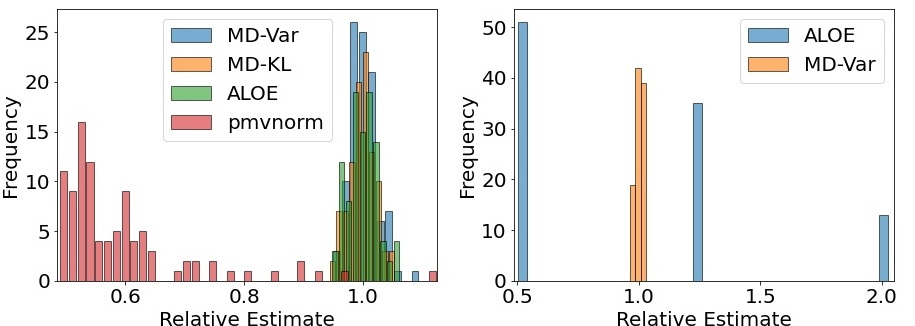
\includegraphics[width=.95\textwidth]{Dissertation/images/sampling/histograms.jpg}
    %\vspace{-.5mm}
    %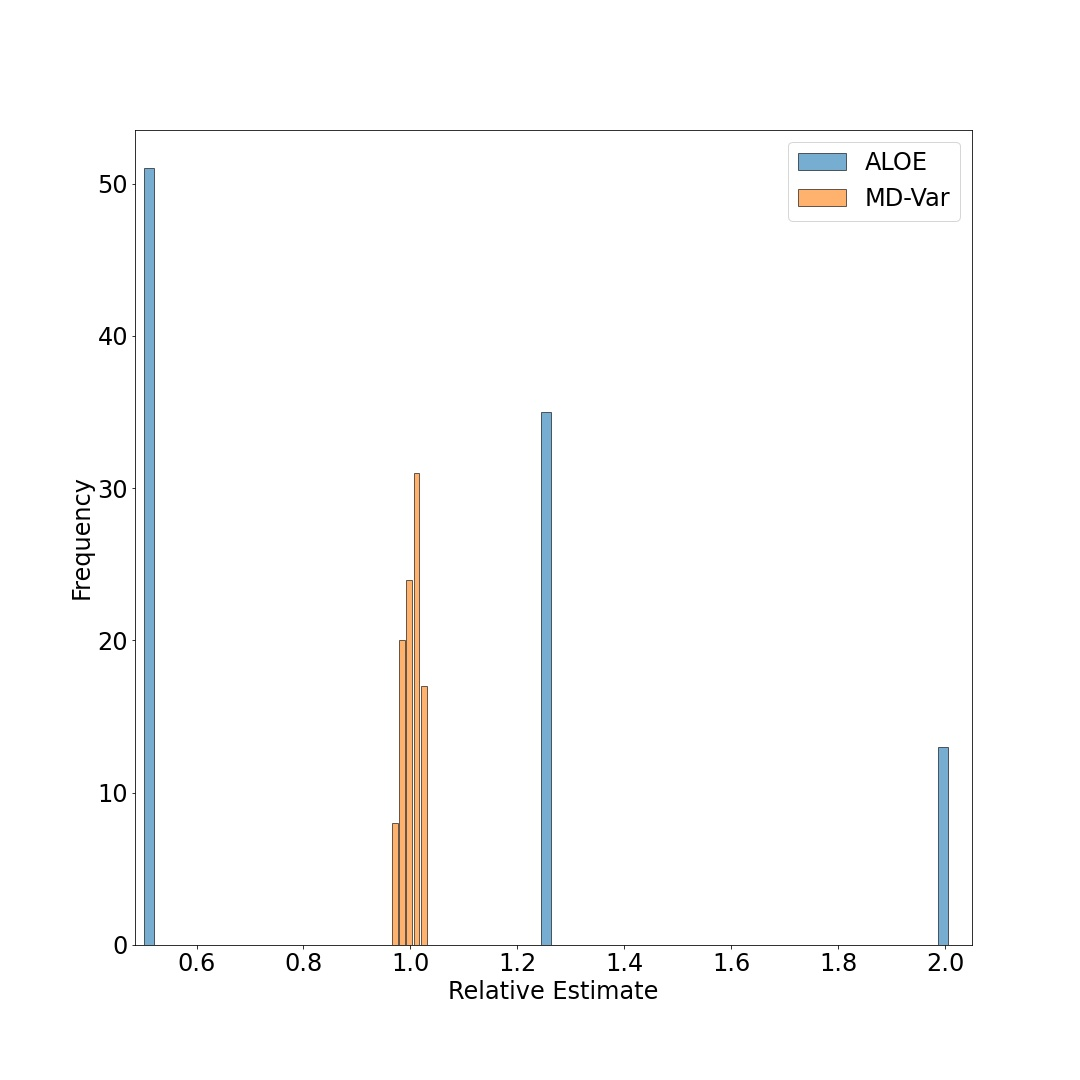
\includegraphics[width=.22\textwidth]{Dissertation/images/sampling/histogram_degenerate.jpg}%\hspace{-3mm}
    %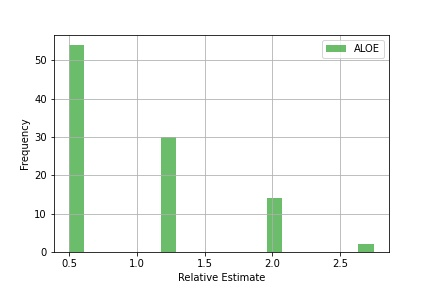
\includegraphics[width=.25\textwidth]{Dissertation/images/sampling/IS_hists_shivering_only_OMC.jpg}
    \caption{Importance 
    sampling methods performance on a 2-dimensional (left) regular polytope with $360$ faces; (right) degenerate polytope with $1500$ faces. Overload probabilities are  $\Phi(-6)$ and $2\Phi(-1)$ resp. 
    }
    \label{fig:01}
    % \vspace{-5mm}
%\end{figure}
%\begin{figure}[t!]
%    \centering
    %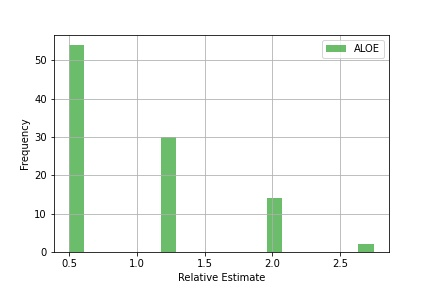
\includegraphics[width=.25\textwidth]{Dissertation/images/sampling/IS_hists_shivering_only_OMC.jpg}
    %\caption{Importance 
    %sampling methods performance on a 2-dimensional degenerate polytope with $1500$ faces and overload probability $2\Phi(-1)$.}
    %\label{fig:degenerate_polytope}
    %\vspace{-5mm}
\end{figure}

%Moreover, we would like to address the question of sampling complexity's dependence on the number of planes and true event probability. See Figure~\ref{fig:complexities}. We declare that the algorithm has converged once the relative difference between two subsequently produced standard deviations of the estimate are small enough: $|\texttt{std}_i - \texttt{std}_{i+1}| / \texttt{std}_{1000} \leq 10^{-3}$. 
%{\color{red} Sasha, please change it as we discuss. The criteria above does not make any sense because of the numerical instability}
%Here we can observe that the smaller probability than it is more samples required to estimate that for MC. ALOE and proposed methods, i.e., Mirror Descent based, seems to be not caring much about the true probability. Also, we observe that the proposed mirror descent based approaches are much more efficient.



\paragraph{Degenerate polytope} Although ALOE is one of the best choices for a regular polytope, the algorithm does not take into account the joint geometry of various hyperplanes. 
%
As the second example we consider a degenerate polytope with $J=1500$ faces, where $\omega_1 = (0, 1)$  and $\omega_j = (\xi, -1 - \xi)$, $2\le j \le J$. We take $\xi \sim \mathcal{U}[-\varepsilon, \varepsilon]$ for small $\varepsilon = 10^{-6}$. Note that $\omega_j$ for $j\geq 2$ are almost identical. Hence probability $\Pi$ is quite close to $2\Phi(-\tau)$. In this experiment, ALOE puts a lot of efforts on sampling points in the area $\{p: (0, -1)^\top p \ge \tau\}$, while the set $\{p: \omega_1^\top p \ge \tau\}$ remains unexplored which leads to a higher variance of the sampler and a less efficient method compared to the proposed optimization approach. Figure~\ref{fig:01} illustrates the performance of ALOE in this case. 

\paragraph{Power Grid Cases} In this subsection we consider real-world polytopes corresponding to DC power grids (IEEE test cases) and Gaussian power injections.
%
%We also compare the algorithms' efficiency in solving the  on various IEEE test cases. s
%by comparing the algorithms' efficiency over various IEEE test cases. 
%
We ran the algorithms on all the test cases  accessible through PandaPower~\cite{pandapower.2018}. There were 27 cases with the number of buses varying from 4 to 9241. The proposed methods (MD-Var and MD-KL) took less than two minutes of computational time on a personal laptop for each of them. 
%
Table~\ref{tab:sample-compX} shows the minimal number of samples that are required by the algorithms to achieve 
\begin{align}
    \Pi/2 \le \hat\Pi \pm s(\hat\Pi) \le 3\Pi/2, \label{eq:tk}
\end{align}
where $s(\hat\Pi)$ is the empirical standard deviation of the estimate. This ensures that not only the estimated value, but also its confidence interval is contained in $(\Pi/2, 3\Pi/2)$ and that the sum of the empirical estimate and its standard deviation are close to %of the same order as 
the true probability. 


\begin{table}[ht]
\centering
%\vspace{-4mm}
\captionsetup{justification=centering}
\caption{Number of samples to satisfy Ineq.~\eqref{eq:tk} 
 for Iceland118}
 \begin{tabular}{c|c|c|c|c} 
 \hspace{-2mm}Bound ${\bar\theta}_{ij}$, probability $\Pi$ & MC & ALOE & Pmvnorm & MD-Var\\
 % &&& \cite{genz2020package} & (Section \ref{sampling:nm})\\
 \hline
  \hspace{-2mm}$|{\theta}_{ij}| \le \pi/8$, $\Pi$ = 1.2e-01 & 6.4e+02 & 3.7e+02 & \underline{3.2e+02} & 4.1e+02\\
  \hspace{-2mm}$|{\theta}_{ij}| \le \pi/7$, $\Pi$ = 3.0e-02 & 5.1e+04 & 4.1e+02 & 1.1e+03 & \underline{3.5e+02}\\
  \hspace{-2mm}$|{\theta}_{ij}| \le \pi/6$, $\Pi$ = 2.5e-03  & 6.2e+06 & 4.5e+02 & 6.3e+03 & \underline{3.9e+02} \\
  \hspace{-2mm}$|{\theta}_{ij}| \le \pi/5$, $\Pi$ = 2.6e-05  & 8.9e+10 & 3.3e+02 & 1.4e+04 & \underline{2.1e+02}\\
 \end{tabular}
 \vspace{-3mm}\label{tab:sample-compX}
\end{table}


Table~\ref{tab:emp} shows overload probability estimates and their standard deviations for the algorithms based on $N = 200$ samples on various PandaPower~\cite{pandapower.2018} power grids. In all the presented cases except for the Iceland grid, we set the standard deviations of output powers of generators to $0.25$ of their average values. For the Iceland test case, we use $0.1$ instead of $0.25.$ 
Pmvnorm~\cite{genz2020package} did not terminate on Polish 3120sp case after an hour of computations which we indicated as N/A. All other methods terminate in less than a minute. The proposed algorithms reduce variance and are more computationally efficient than the state-of-the-art ALOE and pmvnorm. Fig.~\ref{fig:weights118}~shows~a~substantial change in hyperplane weight assignment made by MD-Var. Our code is publicly available on Github at \url{https://github.com/vjugor1/adaptive_importance_sampling_power_grids}. 

%how convex optimization 
%% To reviewers' response
%Another field to be considered is the weights in the mixture. Figure~\ref{fig:weights118} shows the distribution of top weights in the $\textit{MD}_{\textit{V}}$ and ALOE's mixtures for the Iceland118 case with fluctuations of $0.1$ magnitude and maximum phase difference of $\pi / 3$. We have not included $\textit{MD}_{\textit{KL}}$ for the sake of clearer presentation, since it yielded almost the same weights as the $\textit{MD}_{\textit{V}}$. We can observe that the optimization approach brings out the most crucial (from the failure point of view) component higher and leaves the rest almost untouched.

% %To further investigate the variance behaviour, let us see Figure~\ref{fig:3120}. 
% %Here we can see that the proposed algorithms dominate the ALOE in terms of variance thought the whole sampling process. $\textit{MD}_{\textit{V}}$, non-surprisingly, has better variance than $\textit{MD}_{\textit{KL}}$, since the former is aimed at variance optimization.

% %\begin{figure}[h]
% %    \centering
% %    \vspace{-3mm}
% %    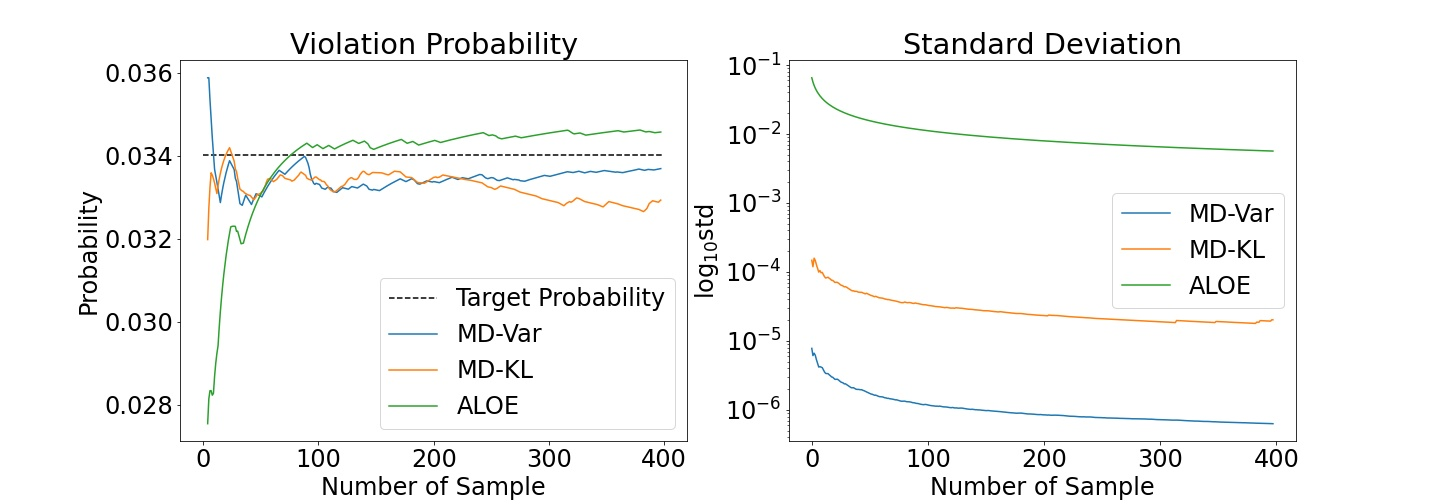
\includegraphics[width=.55\textwidth]{Dissertation/images/sampling/grid3120with_pmv.jpg}
% %    \vspace{-3mm}
% %    \caption{Convergence plots for the probability estimates (left) and standard deviation of the estimates (right) for the Polish3120 grid. Maximum angle difference is $\pi/4$ and the fluctuation are $0.25$ of magnitudes.}
% %    \label{fig:3120}
% %    \vspace{-4mm}
% %\end{figure}


% %Another field to be considered is the weights in the mixture. Figure~\ref{fig:weights118} shows the distribution of top weights in the $\textit{MD}_{\textit{V}}$ and ALOE's mixtures for the Iceland118 case with fluctuations of $0.1$ magnitude and maximum phase difference of $\pi / 3$. We have not included $\textit{MD}_{\textit{KL}}$ for the sake of clearer presentation, since it yielded almost the same weights as the $\textit{MD}_{\textit{V}}$. We can observe that the optimization approach brings out the most crucial (from the failure point of view) component higher and leaves the rest almost untouched.

\begin{figure}[t]
    \centering
    %\vspace{-1mm}
    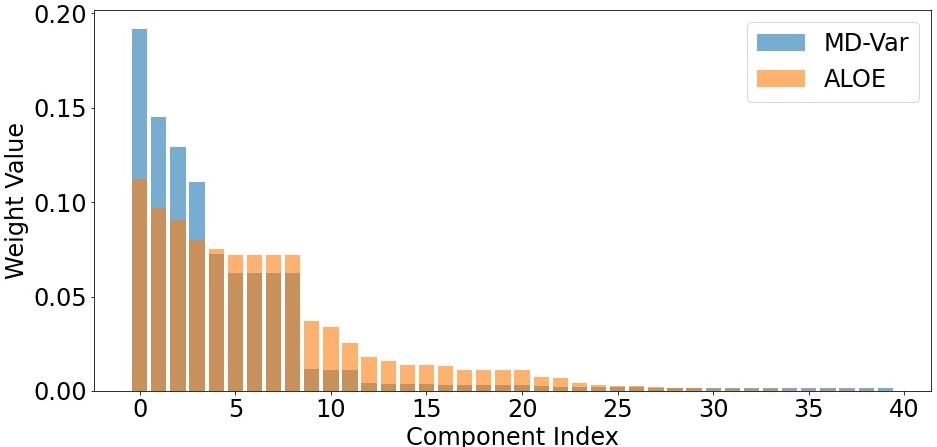
\includegraphics[width=.95\textwidth]{Dissertation/images/sampling/weights_pi3_grid118i.jpg}
    %\vspace{-2mm}
    \captionsetup{justification=centering}
    \caption{Weights of mixture distribution %\eqref{eq:mix} 
    assigned by ALOE and MD-Var for Iceland 118 case with phase angle limit $\pi/3$ and a standard deviation of power injection on generators equal to $0.1$ of its average.}
    \label{fig:weights118}
    % \vspace{-2mm}
\end{figure}



% \begin{comment}
% Finally, as the ground truth we use an estimate of failure given after $N=10000$ iterations of ALOE~\cite{owen2019importance} and set $\Pi$ equal to it in Table~\ref{tab:emp}. We set a deviation on generators (except the slack bus) to be 0.1 of net power injections, i.e. the difference between power generation and consumption. Finally, we set variance on loads equals to zero. \end{comment}




\begin{table}[t]
    \centering
    \captionsetup{justification=centering}
    \caption{Overload probability estimation for power grids.}
    \label{tab:emp}
    {\scriptsize{
    \begin{tabular}{l|l|l|l|l|l|l}
          Estimate, $\hat\Pi$ & $\bar\theta$ & $\Pi$ &  \text{ALOE} & MD-Var & MD-KL & pmvnorm\\
          \hline
          \multicolumn{7}{c}{IEEE 30}\\
          \hline
$\hat\Pi \times$ 1e+15 & $\pi/4$\hspace{-4mm}&8.2\!\! & 8.2 $\pm$ 0.9 & 8.2 $\pm$ 0.0 & 8.2 $\pm$  0.0 & 8.2 $\pm$ 1.2 \\
$\hat\Pi \times$ 1e+06 & $\pi/6$\hspace{-4mm}&5.8\!\! & 5.8 $\pm$ 0.7 & 5.8 $\pm$ 0.0 & 5.8 $\pm$ 0.0 & 5.8 $\pm$ 1.0 \\
$\hat\Pi \times$ 1e+04 & $\pi/7$\hspace{-4mm}&2.9\!\! & 2.9 $\pm$ 0.3 & 2.9 $\pm$ 0.0 & 2.9 $\pm$ 0.0 & 2.9 $\pm$ 0.5\\
$\hat\Pi \times$ 1e+03 & $\pi/8$\hspace{-4mm}&3.1\!\! & 3.1 $\pm$ 0.4 & 3.1 $\pm$ 0.0 & 3.1 $\pm$ 0.1 & 3.1 $\pm$ 0.4\\
\hline
\multicolumn{7}{c}{IEEE 57}\\
\hline
$\hat\Pi \times$ 1e+03 & $\pi/2$\hspace{-4mm}&8.8\!\! & 9.1 $\pm$ 0.8 & 8.7 $\pm$ 0.0 & 8.8 $\pm$ 0.0 & 8.9 $\pm$ 1.2\\
$\hat\Pi \times$ 1e+02 & $\pi/3$\hspace{-4mm}&8.4\!\! & 8.5 $\pm$ 1.1 & 8.4 $\pm$ 0.1 & 8.3 $\pm$ 0.5 & 9.0 $\pm$ 0.9\\
%$\hat\Pi \times$ 1e+01 & $\pi/4$\hspace{-4mm}&2.0\!\! & 2.0 $\pm$ 0.2 & 2.0 $\pm$ 0.0 & 1.9 $\pm$ 0.7 & 2.0 $\pm$ 0.0\\
%$\hat\Pi \times$ 1e+01 & $\pi/6$\hspace{-4mm}&4.1\!\! & 4.1 $\pm$ 0.3 & 4.2 $\pm$ 0.5 & 4.3 $\pm$ 1.0 & 4.1 $\pm$ 0.0\\
          \hline
          \multicolumn{7}{c}{Iceland 118}\\
          \hline
$\hat\Pi \times$ 1e+09 & $\pi/2$\hspace{-4mm}&6.2\!\! & 6.2 $\pm$ 0.1 & 6.1 $\pm$ 0.0 & 6.1 $\pm$ 0.0 & 5.7 $\pm$ 2.6\\
$\hat\Pi \times$ 1e+04 & $\pi/3$\hspace{-4mm}&2.8\!\! & 3.0 $\pm$0.0 & 2.9 $\pm$ 0.0 & 2.9 $\pm$ 0.0 & 2.8 $\pm$ 1.4\\
$\hat\Pi \times$ 1e+02 & $\pi/4$\hspace{-4mm}&1.1\!\! & 1.1 $\pm$ 0.2 & 1.1 $\pm$ 0.0 & 1.1 $\pm$ 0.0 & 1.1 $\pm$ 0.2\\
$\hat\Pi \times$ 1e+01 & $\pi/6$\hspace{-4mm}&1.4\!\! & 1.4 $\pm$ 0.2 & 1.4 $\pm$ 0.0 & 1.3 $\pm$ 0.0 & 1.4 $\pm$ 0.1\\
\hline 
          \multicolumn{7}{c}{Illinois 200}\\
\hline
$\hat\Pi\times$ 1e+12 & $\pi/4$\hspace{-4mm}&7.9\!\! & 7.9 $\pm$ 0.9 & 7.9 $\pm$ 0.0 & 7.9 $\pm$ 0.0 & 7.9 $\pm$ 3.3\\
$\hat\Pi\times$ 1e+04 & $\pi/6$\hspace{-4mm}&1.1\!\! & 1.1 $\pm$ 0.1 & 1.1 $\pm$ 0.0 & 1.1 $\pm$ 0.0 & 1.1 $\pm$ 0.3\\
$\hat\Pi\times$ 1e+03 & $\pi/7$\hspace{-4mm}&2.3\!\! & 2.3 $\pm$ 0.2 & 2.3 $\pm$ 0.0 & 2.3 $\pm$ 0.0 & 2.3 $\pm$ 0.3\\
$\hat\Pi\times$ 1e+02 & $\pi/8$\hspace{-4mm}&1.5\!\! & 1.5 $\pm$ 0.1 & 1.5 $\pm$ 0.0 & 1.5 $\pm$ 0.0 & 1.5 $\pm$ 0.1\\
\hline
\multicolumn{7}{c}{Polish 3120sp}\\
\hline
$\hat\Pi\times$ 1e+13 & $\pi/2$\hspace{-4mm}&3.7\!\! & 3.7 $\pm$ 0.4 & 3.7 $\pm$ 0.0 & 3.7 $\pm$ 0.0 & N/A\\
$\hat\Pi\times$ 1e+04 & $\pi/3$\hspace{-4mm}&1.2\!\! & 1.2 $\pm$ 0.1 & 1.2 $\pm$ 0.0 & 1.2 $\pm$ 0.0 & N/A\\
$\hat\Pi\times$ 1e+02 & $\pi/4$\hspace{-4mm}&3.4\!\! & 3.4 $\pm$ 0.5 & 3.4 $\pm$ 0.3 & 3.4 $\pm$ 0.6 & N/A
    \end{tabular}}
    }
    %\vspace{-4mm}
\end{table}




\section{Conclusion}\label{sampling:conclusion}

Importance sampling is a useful tool for real-time reliability assessment in power grids. We proposed an algorithm that, first, constructs a physics-informed mixture distribution for importance sampling, and, second, utilizes convex optimization to adjust the weights of the mixture.  The method outperforms state-of-the-art algorithms in accuracy and efficiency of reliability assessment. We hope that this approach can be further used for optimization and control in power grids. %importance sampling can ... used for control purposes

% % \bibliographystyle{IEEEtran}
% % \bibliography{biblio}

\chapter{Importance Sampling Approach to Chance Constrained DC-OPF}
This chapter is based on the publication \fullcite{lukashevich2021importance}.
\label{chap:dc_stochastic_approx}

\section{Introduction}

In 2020 electricity produced approximately 25\% of greenhouse gas emissions in the USA, and integration of a higher volume of renewable energy generation is seen as the primary tool to reduce the emission level \cite{hockstad2018inventory}. In turn, a higher amount of renewable generation increases the power grid uncertainty, compromises its security, and challenges classical power grid operation and planning policies \cite{koutsoyiannis2016unavoidable}. 

The optimal power flow (OPF) problem, which determines the economically optimal operating level of power generation under given power balance equations and security constraints, is one of the most fundamental problems in grid operation and planning \cite{stott2012optimal}. Several extensions are proposed for the optimal power flow problem for addressing the uncertainty of power generation and consumption \cite{geng2019data}. Robust and chance-constrained power flow formulations are among the most popular ones. The robust OPF problem assumes bounded uncertainty and requires a solution to be feasible against any possible uncertainty realization within a given uncertainty set~\cite{ben2002robust,ding2016adjustable,sousa2010robust}. 

A more flexible and general chance-constrained approach requires security constraints to be satisfied a high probability while assuming the distribution of renewables is known in whole or in part \cite{lubin2015robust, roald2017chance,bienstock2014chance,pena2020dc,mitrovic2023gp,mitrovic2023data}. We consider a joint chance-constrained optimal power flow problem, where the joint probability of at least one failure of the security constraints (line load limits, voltage stability bounds) is bounded from above by a confidence threshold (JCC-OPF). 

In contrast to a single chance-constrained formulation (SCC-OPF), which imposes individual failure probability thresholds for each of the constraints, the joint chance constraint is computationally hard even for direct current (DC) power balance equations, which is characterized by linear security limits, with Gaussian uncertainty~\cite{cousins2014cubic,khachiyan1993complexity}. Several tractable convex approximations have been proposed \cite{nemirovski2007convex, nemirovski2006scenario,nemirovski2003tractable,trofino1999bi} for joint chance-constrained optimization to overcome the computational hardness of the problem. However, they often lead to conservative solutions inapplicable for operational practice. 

Other approaches such as scenario and sample average approximations \cite{calafiore2006scenario,garatti2019risk, vrakopoulou2013probabilistic,nemirovski2006scenario} consist of substituting the stochastic part with a set of deterministic inequalities based on the uncertainty realization. This approach can be distributionally robust and allow exploiting uncertainties beyond the Gaussian ones. A combination of an analytical approximation and sampling~\cite{hou2020chance} can further improve the accuracy of the solution. However, it may require a large number of samples. Scenario curation/modification heuristics have been designed to improve the sample complexity of JCC-OPF \cite{mezghani2020stochastic}, although without formal analysis of the methodology. In work outside power grids, statistical learning has been used to approximate uncertain convex programs~\cite{vapnik1999overview,maximov2016tight,campi2020scenario}.

Nevertheless, the scenario approximation approach remains the most accurate algorithm for solving the joint chance-constrained DC optimal power flow. At the same time, its complexity is often unacceptable for large-scale power grids~\cite{sakhavand2020new}. To this end, the study suggests using importance sampling to reduce the complexity and improve the accuracy of the scenario approximation to chance-constrained optimal power flow. The importance sampling approach generates more informative samples and results in an optimization problem with fewer constraints. Our study extends earlier results \cite{barrera2016chance,tong2022optimization} on importance sampling for chance-constrained optimization. 

The contribution of the study is as follows. 
\begin{enumerate}
  \item we propose a novel computationally efficient 
  approach to the joint chance-constrained DC OPF problem. The algorithm exploits physics-informed importance sampling to refine the classical scenario approximation~\cite{calafiore2006scenario};
  \item we prove the algorithm to converge to a solution of JCC-DC-OPF with a guaranteed accuracy under mild technical assumptions; 
  \item we demonstrate the proposed algorithm's superior computational efficiency and accuracy relative to standard methods over multiple real and synthetic test cases.
\end{enumerate}

The chapter is organized as follows.
Section~\ref{sec:not} presents the joint chance-constrained optimal power flow problem and introduces the notation used in the chapter. We outline the algorithm and provide its theoretical analysis in Section~\ref{sec:algo}. Empirical study and comparison to state-of-the-art methods are given in Section~\ref{sec:emp}. In Section~\ref{sec:conclusion} we conclude with a summary and critical discussion on possible applications of our results.



\section{Background and Problem Setup}\label{sec:not}

\subsection{Notation}
The direct current (DC) power flow approximation remains extremely popular yet simple model for analysis because of a linear relation between powers and phase angles in typical high-voltage power grids. 

In this study, we consider a power grid given by a graph $\mathcal{G} = (V, E)$ with a set of nodes/buses $V$ and edges/lines $E$. Assume $n+1$ is a number of buses, and $m$ is a number of lines. Let $p$ be a vector of power injections $p = (p_F, p_R, p_S)^\top$, where $p_F$ corresponds to buses with deterministic/fixed (F) power injections, $p_R$ to buses with random (R) injections, and $p_S$ is the injection at the slack bus (S). The power system is balanced, i.e., the sum of all power injections equals to zero, $p_S = -\sum_{r\in R} p_r - \sum_{f\in F} p_f$. Let $B \in \mathbb{R}^{n+1 \times n+1}$ be an admittance matrix of the system, $p = B\theta$. The components $B_{ij}$ are such that $B_{ij} \neq 0$ if there is a line between nodes $i$ and $j$, the diagonal elements $B_{ii} = - \sum_{j\neq i} B_{ij}$, i.e., $B$ is a Laplacian matrix. Let $\theta$ be a vector of phase angles. Thus, $B$ is rank deficient with one eigenvalue equal to $0$. Without a loss of generalization, we assume that the phase angle on the reference slack bus $\theta_S = 0$, and given that the injection $p_S$ is the negative sum of the other injections, we can analyze a \textit{reduced} order system by ignoring the reference bus $S$. This is done by removing the injection and phase angle at $S$ from $p$ and $\theta$, and removing the row and column corresponding to $S$ from $B$. This gives an invertible reduced power-flow model at the non-reference buses \cite{aburbook,dekatcns}. We use $\theta, p, B$ to the reduced quantities and can write their inverse relation as ~$\theta = B^{-1} p$.

The DC power flow equations, generation and stability constraints are
\begin{align}
    & p = B \theta \label{eq:DC-PF-a}\\
    & p^{\min}_i \leq p_i \leq p^{\max}_i, i \in V \label{eq:DC-PF-b}\\
    & |\theta_i - \theta_j| \leq \bar{\theta}_{ij}, \; (i,j)\in E \label{eq:DC-PF-c}
\end{align}
Let $A \in \{-1,0,1 \}^{m \times n}$ be the reduced incidence matrix, i.e., column corresponding to reference bus $S$ is removed, of grid $G$. If nodes $i$ and $j$ are connected by edge $k$ then $A_{ki} = +1$, $A_{jk} = -1$ and all other elements are equal to zero. Then the phase angle constraints in \eqref{eq:DC-PF-c} can be represented as  $AB^{-1}p \le \bar\theta$, $-AB^{-1}p \le \bar\theta$. 

%Let $C \in \mathbb{R}^{n\times n}$ be a symmetric matrix such that for all random nodes $r$, fixed nodes $f$ and the slack node $S$, $C_{rr} = 1$, $C_{ff} = 1$, $C_{Sr} = - 1$, $C_{Sf} = - 1$, while all other elements are equal to zero. 
In DC OPF (Optimal power Flow), we seek to minimize some cost (linear or quadratic), denoted as $\textit{cost}(p)$ on power injections such that the following system of inequalities (operational constraints) are satisfied: 
%{\color{red} \emph{In the description right after formulation (5), the authors assume that the generation cost $\textup{cost}(x,\xi)$ does not depend on the randomness but may depend on the uncertainty distribution. It is a bit confusing to me. Can the authors further explain or give an example to elaborate with more details?}: might be reasonable to address that question here}
\[
\underbrace{(AB^\dagger, - A B^\dagger, I, -I)}_{W}\!\!{}^\top p \le \underbrace{(\bar\theta, \bar\theta, p_{\max}, -p_{\min})}_b\!\!{}^\top,
\]
where $I$ is $n\times n$ identity matrix. Let $J$ be a number of constraints, $J = 2m + 2n$, then $W\in\mathbb{R}^{J\times n}$ and $b\in\mathbb{R}^{n\times 1}$. We refer to the feasibility polytope as the set~$\mathcal{P}$, 
$\mathcal{P} = \bigl\{p:\, Wp \le b\bigr\} = \bigl\{p:\; \bigcap_{i=1}^J\omega_i^\top p \le b_i\bigr\}$.

Finally, we assume that fluctuations of power injections $p$ are Gaussian, $p = x +\xi$, where $\xi$ is a zero mean Gaussian uncertainty, $\xi\sim\mathcal{N}(0, \Sigma)$ and $x$ is the deterministic part of power injections. Under this setting, we solve a joint chance-constrained OPF problem, where the DC-OPF cost is replaced by the expected value $\mathbb{E}_{\sim \xi}\textit{cost}(x,\xi)$ and the operational constraints are now satisfied probabilistically, instead of exactly. This is described in the next section.
% \begin{align}\label{eq:JCC-OPF}
%   \min_x & \;\mathbb{E}_{\xi\sim \mathcal{N}(0, \Sigma)}

The chapter notation is summarized in Table~\ref{tab:notation}. We use lower indices for coordinates of vectors and matrices, lower-case letters for probability density functions (PDFs), and upper-case letters for cumulative distribution functions (CDFs). When it does not lead to a confusion, we use $\mathbb{P}$ and $\mathbb{E}$ to denote probability and expectation without explicitly mentioning a distribution. 

\begin{table}[t]
  \centering
  \begin{tabular}{|p{1.15cm}|p{4.95cm}|p{1.35cm}|p{4.85cm}|}
    $\mathcal{D}$  & $\xi \sim \mathcal{N}(0, \Sigma), ~\xi \notin \mathcal{P}_{\texttt{in}}$ & $\nu(p)$ & PDF of $\mathcal{N}(0, \Sigma)$ without $\mathcal{P}_{\texttt{in}}$ in support \\
    $E$    & set of lines & $q_{D_i}(\xi)$ & mix. component PDF \\
    $V$ & set of buses & $q_D(\xi)$ & mix. distribution PDF \\
    $B$ & admittance matrix& $p^{\max}$ & generation upper limits \\
    $m$ & number of lines & $p^{\min}$ & generation lower limits \\
    $n$ & number of buses & $\mathbb{P}$, $\mathbb{E}$ & probability, expectation \\
    $p$ & power injections & $\mathcal{P_{\texttt{in}}}$ & redundant scen. polytope \\
    $\theta$ & voltage phases & $\mathcal{N}(\cdot, \cdot)$ & Gaussian distribution \\
    $I_n$ & $n\times n$ identity matrix & $\mathcal{P} $ & feas. set  $\{p: Wp\leq b \}$ \\
    $J$ & number of constraints &  $x$ & det. injection $x = \mathbb{E}_\xi p$ \\
    $\bar\theta_{ij}$ & voltage angle limits & $\pi$ & $\mathbb{P}\{\xi \in \mathcal{P}_{\texttt{in}}\}$ \\
    $\xi$ & $\sim\mathcal{N}(0, \Sigma)$ stoch. inj. & $\delta$  & reliability of SA solution \\ 
    $\mathcal{P}_{out}$   & JCC outer approx.  & $\eta$  & confidence level 
  \end{tabular}
  \caption{Chapter notation. }
  \label{tab:notation}
  
\end{table}

\subsection{Problem Setup}
The joint chance-constrained optimal power flow problem~is:
\begin{equation}\label{eq:JCC-OPF}
    \begin{aligned}
  \min_x & \;\mathbb{E}_{\xi\sim \mathcal{N}(0, \Sigma)} \textit{cost}(x,\xi)\\
   \textit{s. t. }\; & \mathbb{P}_{\xi\sim \mathcal{N}(0, \Sigma)} (x+\xi \in \mathcal{P}) \ge 1 - \eta
   \end{aligned}
\end{equation}
where $\eta$ is a preset confidence parameter with $0 < \eta \le 1/2$, and $\textit{cost}(x, \xi)$ is a cost function convex in $x$ for any realization of $\xi$. In other words, we assume that power flow balance equations (Eqs.~\eqref{eq:DC-PF-a}) are satisfied almost surely, and the probability that at least one of the security constraints (Eqs.~\eqref{eq:DC-PF-b} and~\eqref{eq:DC-PF-c}) fails is at most $\eta$. 

Notice that despite the convexity of the cost function of Problem~\eqref{eq:JCC-OPF} is non-convex as its feasibility set is non-convex for a low level of target confidence, i.e., $\eta < 0.5$.

\subsection{Scenario Approach}

Over the last two decades, the scenario approach \cite{nemirovski2006scenario,calafiore2006scenario} 
remains the state-of-the-art method for solving joint chance-constrained optimization. The scenario approach consists in substituting the probabilistic constraints with a large number of deterministic ones with each constraint standing for some uncertainty realization:
\begin{align}\label{eq:sc-opf}
  \min_x & \; \frac{1}{N} \sum_{t=1}^N \textit{cost}(x,\xi^t)\\
  \textit{s. t. } & \; p^{\min} \le x+\xi^t \le p^{\max}, \; 1\le t \le N\nonumber\\
  & \; |\theta_i(\xi^t) - \theta_j(\xi^t)| \le {\bar \theta}_{ij}, (i, j)\in \mathcal{E}, \; 1\le t \le N\nonumber\\
  & x+\xi^t = B \theta(\xi^t), \; 1\le t \le N\nonumber
\end{align}
where $N$ is a number of scenarios, and $\{\xi^t\}_{i=1}^N$ is a set of uncertainty realization. We assume below that the generation cost function $\textit{cost}(x, \xi)$ does not depend on the randomness in power fluctuation ($\textit{cost}(x, \xi) = \textit{cost}(x)$ for any uncertainty realization $\xi$), but may depend on the uncertainty distribution (i.e., on its mean or variance). %{\color{red} Note that dependence of expected cost on known asymptotic parameters of the distribution (variance, mean) are allowed within this framework.}

The key disadvantage of the scenario approximation \eqref{eq:sc-opf} is the number of constraints induced by adding scenarios $\xi^t$. A classical theory, developed by Calafiore and Campi \cite{calafiore2006scenario}, suggests to include a large number of scenarios $N$. This will allow the solution of \eqref{eq:sc-opf} to be feasible for original problem \eqref{eq:JCC-OPF} with high probability $1 - \delta$. However, the number of required scenarios $N$ is given by $N \geq 2 \left( \frac{\ln{1/\delta}}{\eta} + d + d\frac{\ln{1/\eta}}{\eta} \right)$, where $d$ is the number of control variable in the optimization problem. For example, with $\eta = 10^{-2}, \delta = 10^{-2}$, for  IEEE-57 case one would end up with $6.45 \cdot 10^3$ (6 generators, excluding slack one) constraints which is time- and memory-consuming to solve.
% \yury{Is that correct?}
% \sasha{Why not? I have estimated these numbers using Campi's theorem and used number of constraints from IEEE-54}

The major contribution of this chapter is a significant reduction of the requirement on the number of samples by sampling the most informative scenarios. The latter reduces the computational complexity of the scenario approximation and comes up with tight accuracy guarantees for the joint chance-constrained DC optimal power flow problem. 

% and keeping the theoretical guarantees. It is achieved by picking samples from distribution that does not contain ''weak'' samples within its domain. Next, we show that solving scenario approximation with those samples provides better theoretical guarantees on the number of samples - $N$ and the probability to obtain feasible solution of original JCC problem is  $1 - \beta$.
% We next discuss our method to solve Problem \eqref{eq:sc-opf}.

\section{Algorithm}\label{sec:algo}

\subsection{Idea and Sketch}
Our algorithm consists of several steps: 
(1) constructing an inner approximation to the feasibility set,
(2) generating samples outside of this approximation,
(3) and, finally, solving the scenario approximation Problem \eqref{eq:sc-opf} with the generated collection of samples.

First, using the fact that \emph{the probability of a union of events is bounded from below by the maximum of individual event probabilities}, we construct a lower bound on the probability of constraint feasibility $\mathbb{P}(x+\xi \in \mathcal{P})$. The latter allows to add a set of constraints, $x\in \mathcal{P}_{out}$, so that if $x\not\in \mathcal{P}_{out}$ then $\mathbb{P}(x+\xi \notin \mathcal{P}) > \eta$. In other words, if the solution $\bar x$ of the scenario approximation~ \eqref{eq:sc-opf} with samples from the nominal distribution $\mathcal{N}(0,\Sigma)$ satisfies $\mathbb{P}(x+\xi \in \mathcal{P}) \ge 1-\eta$, then adding additional inequalities $x\in \mathcal{P}_{out}$ does not change $\bar x$. Second, using the aforementioned bound, we design a polytope $\mathcal{P}_{\texttt{in}}(x) = \{p: W_{\texttt{in}} \xi \le b_{\texttt{in}}, p = x+\xi\}$ around $x$ with $W_{\texttt{in}}$ and $b_{\texttt{in}}$ independent of $x$. We present the exact expressions for $W_{\texttt{in}}$ and $b_{\texttt{in}}$ in Theorem \ref{thm:20}. Figure~\ref{fig:10} illustrates the idea. 

Then, we show that for any sample $\xi^t$ and feasible $x$, if $p = x+\xi^t \in \mathcal{P}_{\texttt{in}}(x)$, then $p$ also necessarily belongs to the constraint feasibility set $\mathcal{P}$. To this end scenarios $\xi^t: x+\xi^t \in \mathcal{P}_{\texttt{in}}$ can be eliminated from the optimization problem (see Eq.~\eqref{eq:sc-opf}) without impacting the approximation accuracy. 
\def\shift{2.7}
\def\shiftt{2.35}
\def\shiftuselesssample{0.3}
\def\shiftusefulsample{1.1}
\begin{figure}
    \centering
        \begin{tikzpicture}[scale=0.55, node distance={15mm}, thick, main/.style = {draw, scale=.9}] 
        %x
        \coordinate (x) at (0, 0);
        \draw (x) circle (1pt);
        \draw (x) ++(0.05, 0.05) node[above right] (tmp) {$x$};
        %x2
        \coordinate (x2) at (0 + \shiftt, 0 - \shiftt);
        \draw (x2) circle (1pt);
        \draw (x2) ++(0.05, 0.05) node[above right] (tmp) {$x^*$};
        %outer guy
        \coordinate (a) at ( 4.755282581475767 , 1.545084971874737 );
        \coordinate (b) at ( 3.061616997868383e-16 , 5.0 );
        \coordinate (c) at ( -4.755282581475767 , 1.5450849718747375 );
        \coordinate (d) at ( -2.9389262614623664 , -4.045084971874736 );
        \coordinate (e) at ( 2.9389262614623646 , -4.045084971874738 );
        %linking outer guy
        \draw (a) -- (b);
        \draw (b) -- (c);
        \draw (c) -- (d);
        \draw (d) -- (e);
        \draw (e) -- (a);
        %annotating outer guy
        \draw
        (a) ++(0.1, 0.01) node[above] (tmp) {$\mathcal{P}$};
        %(tmp.west) -- (PO);
        
        %green guy
        \coordinate (ag) at ( 3.804226065180614 , 1.2360679774997896 );
        \coordinate (bg) at ( 2.4492935982947064e-16 , 4.0 );
        \coordinate (cg) at ( -3.804226065180614 , 1.23606797749979 );
        \coordinate (dg) at ( -2.351141009169893 , -3.2360679774997894 );
        \coordinate (eg) at ( 2.3511410091698917 , -3.2360679774997902 );
        %linking green guy
        \draw [olive] (ag) -- (bg);
        \draw [olive] (bg) -- (cg);
        \draw [olive] (cg) -- (dg);
        \draw [olive] (dg) -- (eg);
        \draw [olive] (eg) -- (ag);
        %annotating green guy
        \draw
        (bg) ++(0.1, 0.01) node[below, olive] (tmp) {$\mathcal{P}_{out}$};
        %(tmp.west) -- (PO);
        
        %red guy
        \coordinate (ar) at ( 0.9510565162951535 , 0.3090169943749474 );
        \coordinate (br) at ( 6.123233995736766e-17 , 1.0 );
        \coordinate (cr) at ( -0.9510565162951535 , 0.3090169943749475 );
        \coordinate (dr) at ( -0.5877852522924732 , -0.8090169943749473 );
        \coordinate (er) at ( 0.5877852522924729 , -0.8090169943749476 );
        %linking red guy
        \draw [red] (ar) -- (br);
        \draw [red] (br) -- (cr);
        \draw [red] (cr) -- (dr);
        \draw [red] (dr) -- (er);
        \draw [red] (er) -- (ar);
        %annotating red guy
        \draw
        (br) ++(1em, .1em) node[above right, red] (tmp) {$\mathcal{P}_{\texttt{in}}(x)$};
        %(tmp.west) -- (PO);
        
        %red guy2
        \coordinate (ar2) at ( 0.9510565162951535 + \shiftt , 0.3090169943749474 - \shiftt);
        \coordinate (br2) at ( 6.123233995736766e-17 + \shiftt , 1.0  - \shiftt);
        \coordinate (cr2) at ( -0.9510565162951535  + \shiftt, 0.3090169943749475  - \shiftt);
        \coordinate (dr2) at ( -0.5877852522924732 + \shiftt, -0.8090169943749473 - \shiftt);
        \coordinate (er2) at ( 0.5877852522924729 + \shiftt, -0.8090169943749476  - \shiftt);
        %linking red guy
        \draw [red] (ar2) -- (br2);
        \draw [red] (br2) -- (cr2);
        \draw [red] (cr2) -- (dr2);
        \draw [red] (dr2) -- (er2);
        \draw [red] (er2) -- (ar2);
        %annotating red guy
        \draw
        (br2) ++(1em, .1em) node[above, red] (tmp) {$\mathcal{P}_{\texttt{in}}(x^*)$};
        %(tmp.west) -- (PO);
        
        %Upper \Delta_i
        \coordinate (b_) at (1, 5.7265);
        \draw
        (b_) node[above right] (tmp) {$\Delta_i$};
        %(tmp.west) -- (PO);
        \coordinate (bg_) at (1.5, 5.0898);
        \draw [dashed] (b) -- (b_);
        \draw [dashed] (bg) -- (bg_);
        \draw [thick, black, -latex'] (b_) -- (bg_);
        \draw [thick, black, -latex'] (bg_) -- (b_);
        
        %Inner \Delta_i
        \coordinate (br_) at (-1.5, -0.0898137920080413);
        \draw
        (br_) node[above left] (tmp) {$\Delta_i$};
        %(tmp.west) -- (PO);
        \coordinate (x0_) at (-1.0, -0.7265425280053608);%x!
        \draw [dashed] (br) -- (br_);
        \draw [dashed] (x) -- (x0_);
        \draw [thick, black, -latex'] (br_) -- (x0_);
        \draw [thick, black, -latex'] (x0_) -- (br_);
        
        %Inner \Delta_i 2
        \coordinate (br_2) at (-1.5 + \shiftt, -0.0898137920080413 - \shiftt);
        \draw
        (br_2) node[above left] (tmp) {$\Delta_i$};
        %(tmp.west) -- (PO);
        \coordinate (x0_2) at (-1.0 + \shiftt, -0.7265425280053608-  \shiftt);%x!
        \draw [dashed] (br2) -- (br_2);
        \draw [dashed] (x2) -- (x0_2);
        \draw [thick, black, -latex'] (br_2) -- (x0_2);
        \draw [thick, black, -latex'] (x0_2) -- (br_2);
        
        % Samples
        %% Useless
        \coordinate (xu_1) at (\shiftt + \shiftusefulsample * 0.1, -\shiftt - 3.5*\shiftuselesssample);
        \draw [teal] (xu_1) circle (1pt);
        \coordinate (xu_2) at (\shiftt + \shiftusefulsample, -\shiftt + \shiftusefulsample * 0.5);
        \draw [teal] (xu_2) circle (1pt);
        \coordinate (xu_3) at (\shiftt - \shiftusefulsample * 0.2, -\shiftt + \shiftusefulsample);
        \draw [teal] (xu_3) circle (1pt);
        \coordinate (xu_4) at (\shiftt + \shiftusefulsample * 0.7, -\shiftt - \shiftusefulsample);
        \draw [teal] (xu_4) circle (1pt);
        \end{tikzpicture}  
   
%   \caption{We consider an operating point $x$ and derive a polytope $\mathcal{P}_{out}$ (over the mean level of power injections, $x$) so that no optimal solution $x^*$ of Prob.~ \eqref{eq:JCC-OPF} belongs to $x^*\in\mathcal{P}\setminus \mathcal{P}_{out}$. As it is shown on the figure, polytope $\mathcal{P}_{out}$ (over $x$) induces a polytope $\mathcal{P}_{\texttt{in}}$ (over power injections $p$, $p = x + \xi$) so that none of uncertainty realizations $\xi$ s.t. $p = x+\xi\in\mathcal{P}_{\texttt{in}}$ affect the scenario approximation solution. }

\caption{We consider a deterministic feasibility set $\mathcal{P}$ and derive a polytope $\mathcal{P}_{out}$ inside of it so that no optimal solution $x^*$ of Prob.~ \eqref{eq:JCC-OPF} belongs to $\mathcal{P}\setminus \mathcal{P}_{out}$. The polytope $\mathcal{P}_{\texttt{in}}(x)$ depicts the distances between the planes of $\mathcal{P}$ and $\mathcal{P}_{out}$ for each $x$.
%The polytope $\mathcal{P}_{\texttt{in}}$, defined in terms of noise $\xi$ only, $.
Samples of uncertainty outside $\mathcal{P}_{\texttt{in}}(0)$ are used to determine optimal solution using importance sampling, which will be discussed in detail in Section~\ref{sec:obs}.}
  \label{fig:10}
  %\vspace
\end{figure}

Finally, we sample scenarios outside of the polytope $\mathcal{P}_{\texttt{in}}$ using the state-of-the-art importance sampling methods \cite{owen2019importance,lukashevich2021power} and solve the Scenario Approximation Problem~\eqref{eq:sc-opf} with the collection of samples generated from importance distribution. Later in this section, we provide rigorous proof of the algorithm's efficiency and justify its empirical performance in Section~\ref{sec:emp}. 

\subsection{Inner Approximation}

Consider a probability for the power generation $p$ of being inside the feasibility polytope, $p\in \mathcal{P}$:
\begin{align*}
  \mathbb{P}&(p\in \mathcal{P}) = 
  \mathbb{P}(p: Wp \le b) = \\
  & \mathbb{P}\left(p: \bigcap_{i=1}^J \omega_i^\top p \le b_i\right) = 1 - \mathbb{P}\left(p: \bigcup_{i=1}^J \omega_i^\top p > b_i\right)\le\\
  %
  & 1 - \max_{1\le i\le J}\mathbb{P}\left(p: \omega_i^\top p > b_i\right).
\end{align*}

So, if there exists $x$ such that for some $i$, $\mathbb{P}(\omega_i^\top p > b_i) > \eta$, then $\mathbb{P}(p\in \mathcal{P}) < 1-\eta$. Thus, to satisfy the joint chance constraint for $p = x+\xi$, $\xi\sim \mathcal{N}(0, \Sigma)$, we need

\begin{align}
  \eta \;\ge\; & \mathbb{P}(\omega_i^\top p > b_i) = \mathbb{P}(\omega_i^\top \xi + \omega_i^\top x > b_i) = \nonumber\\
  & 
  \mathbb{P}\left(\frac{\omega_i^\top \xi}{\|\Sigma^{1/2}\omega_i\|_2} > \frac{b_i - \omega_i^\top x}{\|\Sigma^{1/2}\omega_i\|_2}\right) = \nonumber\\
  & \mathbb{P}\left(\zeta > \frac{b_i - \omega_i^\top x}{\|\Sigma^{1/2}\omega_i\|_2}\right) = \Phi\left(\frac{\omega_i^\top x - b_i}{\|\Sigma^{1/2}\omega_i\|_2}\right), \label{eq:cnv}
\end{align}

where $\zeta\sim \mathcal{N}(0,1)$, $\Phi$ is the CDF of the standard normal distribution. Notice, that the function $\Phi(\cdot)$ is convex if its argument is negative, consequently, Ineq.~\eqref{eq:cnv} is convex if~$x\in \mathcal{P}$. 

A set of inequalities $\eta \ge \Phi\left((\omega_i^\top x - b_i)/(\|\Sigma^{1/2}\omega_i\|_2)\right)$, $1\le i \le J$, defines a polytope $\mathcal{P}_{out}$ as follows: 

\begin{align}\label{eq:05}
  P_{out} = \left\{x: \omega_i^\top x \le b_i - \Delta_i, 1\leq i\leq J\right\},
\end{align}

where $\Delta_i = \|\Sigma^{1/2}\omega_i\|_2 \Phi^{-1}(1-\eta)$, $\eta \le 1/2$. %In other words, the operational point $x$ can not be too close to the feasibility boundary to meet the security constraints with a high probability. 
Figure~\ref{fig:10} illustrates mutual arrangement of the polytopes $\mathcal{P}_{out} \subset\mathcal{P}$. Note that $\mathcal{P}_{out}$ defines an outer approximation of the chance-constrained feasibility set, which is itself an inner approximation of the constraint feasiblity set without any uncertainty. Eq.~\eqref{eq:05} implies 
Theorem~\ref{thm:10}.
\begin{theorem}\label{thm:10}
  The joint chance-constrained optimal power flow problem~ \eqref{eq:JCC-OPF} has the same set of optimal solutions as 
  \begin{align}\label{eq:JCC-OPF-Ad}
  \min_x & \;\mathbb{E}_{\xi\sim \mathcal{N}(0, \Sigma)} \textit{cost}(x,\xi)\\
   \textit{s. t. }\; & \mathbb{P}_{\xi\sim \mathcal{N}(0, \Sigma)} (x+\xi \in \mathcal{P}) \ge 1 - \eta, 0 < \eta \le 1/2,\nonumber\\
   & \; x\in \mathcal{P}_{out}\nonumber 
\end{align}
\end{theorem}
\begin{proof}
%{\color{red}Sasha \& Slava, pls add a proof, almost just a refs to Eq.~\eqref{eq:05}.}
A set of additional equations $x\in\mathcal{P}_{out}$ does not affect the solution of Problem~$\eqref{eq:JCC-OPF}$ because the feasiblity set of the chance-constrained optimization problem is inside $\mathcal{P}_{out}$, since the probability for a scenario to be outside of the polytope $\mathcal{P}$ is lower bounded by the probability of being outside of its single face. The latter determines polytope $\mathcal{P}_{out}$, see. Eq.~\ref{eq:05} for details. 
%Eq.~\eqref{eq:05} implies that any optimal solution of  \eqref{eq:JCC-OPF} is also a solution to  \eqref{eq:JCC-OPF-Ad} according to the definition of $\mathcal{P}_{out}$. Moreover, any solution of the Problem~ \eqref{eq:JCC-OPF-Ad} is feasible for Problem~ \eqref{eq:JCC-OPF} and have the same objective. The latter implies that the sets of solutions for~ \eqref{eq:JCC-OPF} and~ \eqref{eq:JCC-OPF-Ad} are the same. 
%
%First, a set of the optimal solutions of \ref{eq:JCC-OPF-Ad} with additional deterministic constraints $x\in \mathcal{P}_{out}$ is a subset of the set of solution of \ref{eq:JCC-OPF}. In this case, according to the definition of $\mathcal{P}_o$, the optimal solution is inside of $\mathcal{P}_o$. Thus, with addition of constraint $ x \in \mathcal{P}_o$, the set of optimal solutions $X$ remains the same.
%Now consider a problem with probabilistic constraints. Let $\tilde{\mathcal{P}_o}$ be a new set of optimal solutions. Since we assume the feasibility of optimal solutions, $\tilde{\mathcal{P}_o} \subset \mathcal{P}_o $ holds. Therefore, in this case addition of constraint $ x \in \mathcal{P}_o$ also does not make any changes in the set of optimal solutions. 
\end{proof}

%\textcolor{red}{Can we jsut nto say that given $\matcal{P}_m$ is outer approximation of the cc-opf feasiblity set it is not going to give any different solution than the cc-opf?}

% \begin{figure}[!t]
%   \centering

%   \includegraphics[width=.45\textwidth]{figure10.jpg}
%   \caption{
%   {\color{red} Sasha, Slava, pls make exactly the same figure with TikZ and put it here}
%   We consider operating point $x$ and derive a derive a polytope $\mathcal{P}_{out}$ so that no optimal solution of Prob.~\ref{eq:JCC-OPF} belongs to $\mathcal{P}\setminus \mathcal{P}_{out}$. As it is shown on the figure, $\mathcal{P}_{out}$ induces a polytope $\mathcal{P}_{\texttt{in}}$ so that none of the power generations $p\in\mathcal{P}_{\texttt{in}}$ affect the scenario approximation solution. } 
%   \label{fig:10}
% \end{figure}




\subsection{Redundant Scenarios}\label{sec:obs}

Another practical consequence of the fact that the optimal solution of the chance-constrained optimal power flow problem is well separated from the boundary of polytope $\mathcal{P}$ is that some scenarios may be removed as they do not improve the accuracy of scenario approximation \eqref{eq:sc-opf}.

Let the optimal solution $\bar x$ of the problem~\eqref{eq:sc-opf} be feasible for the chance-constrained OPF problem. Then by Theorem~\ref{thm:10}, it necessarily belongs to $\mathcal{P}_{out}$. Theorem~\ref{thm:20} provides a mathematical justification of the latter.


\begin{theorem}\label{thm:20}
Any solution of the Scenario approximation problem~ \eqref{eq:sc-opf} that is feasible for the Chance-constrained OPF problem~ \eqref{eq:JCC-OPF} is also a solution of 
%\newpage
%\begin{align}\label{eq:30}
\begin{subequations}
\label{eq:Fin}
  \begin{equation}
  \min_x \; \textit{cost}(x)\nonumber
  \end{equation}
  \begin{equation}
  \hspace{-20mm}\textit{s. t. }\;\; p^{\min} \le x+\xi^t \le p^{\max}, \; 1\le t \le N\label{eq:Fin-a}
  \end{equation}
  \begin{equation}
   \hspace{11mm} |\theta_i(\xi^t) - \theta_j(\xi^t)| \le {\bar \theta}_{ij}, (i, j)\in \mathcal{E}, \; 1\le t \le N\label{eq:Fin-b}
  \end{equation}
  \begin{equation}
  \hspace{-19mm} x+\xi^t = B \theta(\xi^t), \; 1\le t \le N\label{eq:Fin-c}
  \end{equation}
  \begin{equation}
  \hspace{-50mm} x\in \mathcal{P}_{out} \label{eq:Fin-d}
  \end{equation}
\end{subequations} 
\end{theorem}
\begin{proof}
Let $\mathcal{P}_{\texttt{in}}(x) = \{p = x + \xi: \omega_i^\top \xi \le \Delta_i,  \forall i\le J\}$ with $\Delta_i = \|\Sigma^{1/2}\omega_i\| \Phi^{-1}(1-\eta)$. Notice, that $$\mathcal{P}_{\texttt{in}}(x) = \{p+(x-x_0): p \in\mathcal{P}_{\texttt{in}}(x_0)\} .$$
%
Thus for any $x\in \mathcal{P}_{out}$, if $\xi^t\in \mathcal{P}_{\texttt{in}}(0)$ one immediately gets  $p = x+\xi^t \in \mathcal{P}$. In other words, one can exclude scenario $\xi \in \mathcal{P}_{\texttt{in}}(0)$ from Problem~ \eqref{eq:sc-opf} if $p = x+\xi \in \mathcal{P}$. Removing them gives us Problem \ref{eq:Fin}.
\end{proof}
Throughout the chapter, using notation $\mathcal{P}_{\texttt{in}}$ without specifying argument, we assume that it is $\mathcal{P}_{\texttt{in}}(0)$.
Figure~\ref{fig:10} illustrates the idea and the geometry of $\mathcal{P}, \mathcal{P}_{out}$, and $\mathcal{P}_{\texttt{in}}$.

% \deep{Deep:ther eis a notational issue here...$\mathcal{P}_{\texttt{in}}$ is defined for $x$ in the figure (atleast looks like it) but in this discussion or everywhere in the chapter it is defined in terms of $\xi$ which is not the same thing.} \sasha{You are right that $\mathcal{P}_{\texttt{in}}$ is defined by $\xi$ only. It does not depend on $x$ (current operating point) and this fact is vital. It is suitable for each $x$ to serve as a ''safety frame''. Just like when you drive a car, if you hit something, first, you hit it with you car ($\mathcal{P}_{\texttt{in}}$) not your body ($x$). Moreover, that fact that $\mathcal{P}_{\texttt{in}}$ does not depend on $x$ allows one to use samples drawn outside of it for each $x$ with no bias. Otherwise, if $\mathcal{P}_{\texttt{in}}$ would have been depending on $x$, one would samples some scenarios at initial guess $x_0$, then, alongside optimization, those samples would become irrelevant or unrealistic. I hope I answered your question, if not, let us discuss it via emails or in zoom.}

% \deep{Deep: ya I got that,. i meant in the figure it is not clear that it is independent of x ..I dunno if we should draw another box to show that it is only noise/randomness dependent}
% \yury{Corrected/commented right above your comments}
% \sasha{Deep, based on your concern, I extended the example to show and stress 1) independence of $\mathcal{P}_{\texttt{in}}$ of $x$; 2) the implications of constructing SA on samples outside of $\mathcal{P}_{\texttt{in}}$. Need some feedback on design, coloring, etc.}

The following Theorem~\ref{thm:40} follows from the result of Calafiore and Campi~\cite{calafiore2006scenario} and establishes approximation properties of a solution of the Problem~\eqref{eq:Fin}. Assumption~\ref{asmp:10} is the main technical assumption used in the proof of Theorem~\ref{thm:40}.

\begin{assumption}\label{asmp:10}
Assume that for all possible uncertainty realizations $\xi^1, \dots, \xi^N$, the optimization problem \eqref{eq:Fin} is either infeasible or, if feasible, it attains a unique optimal solution.
\end{assumption}

\begin{theorem}\label{thm:40}
Let $\bar x_N$ be a unique solution of the Scenario optimization Problem~\eqref{eq:Fin} with $N$ i.i.d. samples, so that none of the samples belong to $\mathcal{P}_{\texttt{in}}$. Moreover, assume that for any $N$ the assumption \ref{asmp:10} is fulfilled. Then for any $\delta \in (0,1)$ and any~$\eta \in (0, 1/2]$, $\bar x_N$ is also a solution for the Chance-constrained optimal power flow Problem~\eqref{eq:JCC-OPF} with probability at least $1-\delta$ if 
\begin{align*}
  N \ge \left\lceil 2\frac{(1-\pi)\ln \frac{1}{\delta}}{\eta} + 2d + 2d (1-\pi) \frac{\ln\frac{2(1-\pi)}{\eta}}{\eta} \right\rceil, 
\end{align*} 
where $d$ is a dimension of the space of controllable generators, and $\pi$ is the probability of a random scenario $\xi\sim \mathcal{N}(0, \Sigma)$ to belong to $\mathcal{P}_{\texttt{in}}$, and $\pi < 1$. 
\end{theorem}
%\textcolor{red}{Deep: should we say $\mathcal{P}_{\texttt{in}}$ or $\mathcal{P}_{\texttt{in}}(0)$ or mention that from now on that we will follow the notation where we avoid mentioning the x as x=0 (mentioned after the proof of Theorem 3.2)? A reviewer also mentioned. If yes, Sascha please change or add (x) or (0), wherever it is needed.}
\begin{proof}
First, notice that discarding random scenarios $\xi\notin \mathcal{P}_{\texttt{in}}$ is equivalent in solving the scenario approximation problem with sampling $\xi$ from a distribution $\mathcal{D}$ where  $\xi \sim \mathcal{D} \Leftrightarrow \xi\sim \mathcal{N}(0, \Sigma) \textit{s. t. } \xi\not\in \mathcal{P}_{\texttt{in}}$. From the theorem statement, $1-\pi$ is the probability mass associated with samples in $\xi\sim \mathcal{N}(0, \Sigma)$ that are outside $\mathcal{P}_{\texttt{in}}$.

According to the result of Calafiori and Campi~\cite{calafiore2006scenario}, for any probability $\delta\in (0,1)$ and any confidence threshold probability $\varepsilon$, and dimension of the space of parameters $d$ one has, for~$N_1$
\begin{align}\label{eq:mon}
  N_1 \ge \left\lceil \frac{2}{\varepsilon} \ln \frac{1}{\delta} + 2d + \frac{2d}{\varepsilon} \ln \frac{2}{\varepsilon}\right\rceil 
\end{align}
scenarios from $\mathcal{D}$ and the optimal solution 
$\bar x$ of the Problem~\eqref{eq:Fin}, 
%(\textcolor{red}{or (9)?})
the probability of failure is bounded as
\begin{align*}
  \mathbb{P}_D(\bar{x}\not\in \mathcal{P}) \le \varepsilon
\end{align*}
with probability at least $1-\delta$. 

Notice, that the bounds on the number of samples (see Eq.~\eqref{eq:mon}) is strictly decreasing in $\varepsilon$ for $\varepsilon \in (0,1)$. As scenarios in $\mathcal{P}_{\texttt{in}}$ do not cause failure, to get a probability of failure $\eta$ according to measure $\mathcal{N}(0, \Sigma)$, we need the failure probability according to $D$ to be at least $\varepsilon = \eta/(1-\pi)$.  
Thus, taking $\varepsilon = \eta/(1-\pi)$ and using monotonicity of~Ineq.~\eqref{eq:mon} one gets the statement of the theorem. 
\end{proof}

Theorem~\ref{thm:40} establishes the number of scenarios sufficient for the scenario approximation solution being feasible for the chance-constrained optimal power flow problem. This number significantly decreases if one can come up with a sufficiently restrictive inner approximation of the feasibility set, that is close to the true chance-constrained set. Notice, that without an inner approximation, i.e., for $\pi = 0$, one gets the result of Calafiore and Campi~\cite[Theorem 1]{calafiore2006scenario}. %Similarly, for $\pi=1$ the upper bound on the number of scenarios tends to infinity as all samples are generated outside of the feasibility set $\mathcal{P} = \mathcal{P}_{out} = \mathcal{P}_{\texttt{in}}$ and the problem is infeasible for any finite number of samples. 

\subsection{Importance Sampling}

Although a scenario optimization with scenarios that do not belong to the polytope $\mathcal{P}_{\texttt{in}}$ obey a nice complexity bound, it requires on average $1/(1-\pi)$ or more samples to generate at least one point outside of $\mathcal{P}_{\texttt{in}}$ and decreases the overall efficiency of the approach. The problem is especially challenging when dealing with rare events, i.e., the confidence level $\eta \to 0$. 

Importance sampling is a general technique that helps to improve the efficiency of scenario generation~\cite{tokdar2010importance}. It consists of changing the probability distribution to sample rare events with a higher probability. Figure~\ref{fig:20} illustrates the concept. 

% \begin{figure}[!t]
%   \centering

%   \includegraphics[width=.45\textwidth]{figure20.jpg}
%   \caption{
%   {\color{red} Sasha, Slava, pls make exactly the same figure with TikZ and put it here}
%   Our goal is to sample points in the area $\{x: f(x) = 1\}$. Sampling from the nominal distribution $\phi(x)$ is inefficient as one needs to sample from the distribution tail. The probability distribution $\psi(x)$ is a better choice as the probability of getting $f(x) = 1$ is substantially higher when sampling from it.} 
%   \label{fig:20}
% \end{figure}

\pgfmathdeclarefunction{gauss}{3}{%
 \pgfmathparse{#3/(#2*sqrt(2*pi))*exp(-((x-#1)^2)/(2*#2^2))}%
}
\begin{figure}[ht]
  \centering

\begin{tikzpicture}[scale=0.63]
\begin{axis}[
 no markers, domain=-2:2, samples=100,
 axis lines*=left, xlabel=$x$,
 height=5cm, width=12cm,
 xtick={0,1}, ytick=\empty,
 enlargelimits=false, clip=false, axis on top,
 grid = major
 ]
 %\addplot [fill=cyan!20, draw=none, domain=0:5.96] {gauss(6.5,1)} \closedcycle;
 %\addplot [very thick,cyan!50!black] {gauss(4,1)};
 \addplot+[very thick,cyan!50!black] {gauss(0,0.53,0.53)} node[above=0.15cm,pos=.5,cyan!50!black] {$\phi(x)$};
 \addplot+[very thick,red] {gauss(1.7,0.3,0.2)} node[above=0.65cm,pos=0.85,red] {$\psi(x)$};
 \addplot+[const plot, no marks, thick] coordinates {(0,0) (1,0.2) (1,0.2) (2,0.2)} node[above left=0.1cm,pos=0.6,olive] {$f(x)$};
\end{axis}

\end{tikzpicture}
\caption{
  Our goal is to sample points in the area $\{x: f(x) = 1\}$. Sampling from the nominal distribution $\phi(x)$ is inefficient as one needs to sample from the distribution tail. The probability distribution $\psi(x)$ is a better choice as the probability of getting $f(x) = 1$ is substantially higher when sampling from it.}

  \label{fig:20}
\end{figure}

Unfortunately, there is no exact and time-efficient algorithm for sampling outside of a convex polytope from Gaussian distribution \cite{khachiyan1993complexity}. However, the ALOE algorithm~\cite{owen2019importance,lukashevich2021power} proposes an elegant way for approximating the distribution of interest by sampling from a mixture of distributions. 

We consider Gaussian fluctuations of power injections, $\xi \sim \mathcal{N}(0, \Sigma)$, with known covariance $\Sigma \in \mathbb{R}^{n\times n}$ and aim to sample scenarios outside of $\mathcal{P}_{\texttt{in}}$ so that the probability distribution to sample from is as close as possible to the conditional Gaussian distribution $\xi \sim \mathcal{N}(0, \Sigma) \textit{s. t. } \xi\not\in \mathcal{P}_{\texttt{in}}$. 

The method essentially samples from a weighted mixture of conditional Gaussian distributions $D_i$ 
\[\xi \sim D_i \Longleftrightarrow \xi \sim \mathcal{N}(0, \Sigma) \textit{s. t. } \omega_i^\top \xi > \Delta_i. \]

Consider the set of inequalities $\{\omega_i^\top \xi > \Delta_i\}_{i\le J}$ in more detail. First, let $\zeta \sim \mathcal{N}(0, I_n)$ then the system is equivalent to $\{(\Sigma^{1/2}\omega_i)^\top 
\zeta > \Delta_i\}_{i\le J}$. 


Distribution $D_i$ can be simulated exactly using the inverse transform method \cite{l2009monte,morlet1983sampling} that admits conditional sampling $\xi \sim \mathcal{N}(0, \Sigma)$ s.t. $\omega_i^\top \xi \ge \Delta_i$. 
\begin{enumerate}
  \item Sample $z \sim \mathcal{N}(0, I)$ and sample $u \sim U(0,1)$
  \item Compute $y = \Phi^{-1}(\Phi(-\Delta_i) + u(1 - \Phi(-\Delta_i)))$
  \item Set $\phi = \phi y + (I - \phi\phi^\top) z$, $\phi = \Sigma^{1/2} \omega_i / \|\Sigma^{1/2} \omega_i\|_2$
  \item Set $\xi = \Sigma^{1/2} \phi$.
\end{enumerate}

In \cite{owen2019importance,lukashevich2021power}, the authors proposed a slightly refined version of the algorithm above that exhibits better numerical stability. We refer to the same papers for the corresponding proofs and analysis. Figure~\ref{fig:conv_vs_MC} illustrates the idea: the samples can be obtained out of a certain set, e.g., feasibility polytope. In this chapter, $\mathcal{P}_{\texttt{in}}$ (see Figure \ref{fig:10}) will play the role of the set to be sample out of.


Finally, ALOE proposes to sample scenarios from a weighted mixture
\begin{align}\label{eq:q_d}
  D = \sum_{i=1}^J \alpha_i D_i, \; & \alpha_i \ge 0, \sum_{i=1}^J \alpha_i = 1,\nonumber \\
  & \alpha_i \propto \Phi(-\Delta_i/\|\Sigma^{1/2}\omega_i\|_2),
\end{align}
where $\Phi$ is a CDF of the standard normal distribution. Let $q_D(\xi)$ be a PDF of distribution $D$, then Theorem~\ref{thm:50} established a maximal ratio of the conditional Gaussian density~$\xi\sim\mathcal{N}(0, \Sigma) \textit{s. t. } \xi\not\in\mathcal{P}_{\texttt{in}}$ and~$q_D(\xi)$. 

\begin{theorem}\label{thm:50}
Let $\nu(\xi)$, $q_D(\xi)$ be PDFs  of $\xi\sim\mathcal{N}(0, \Sigma) \textit{s. t. } \xi\not\in\mathcal{P}_{\texttt{in}}$, and a mixture density (see Eq.~\eqref{eq:q_d}), resp. Then for any $\xi\not\in\mathcal{P}_{\texttt{in}}$, we have
\begin{align}\label{eq:M}
  \nu(\xi) \le M q_D(\xi),  
  M = \frac{\sum_{i\le J} \Phi(-\Delta_i/\|\Sigma^{1/2}\omega_i\|_2)
  }{\max_{i\le J}\Phi(-\Delta_i/\|\Sigma^{1/2}\omega_i\|_2)}, 
\end{align}
where $D$ and $\alpha_i$ are given in Eq.~\eqref{eq:q_d}.
\end{theorem}
\begin{proof}
Let $\phi(\xi)$ be PDF of $\xi\sim\mathcal{N}(0, \Sigma)$. Notice, that the conditional densities $D_i$ have probability density functions 
\[q_{D_i}(\xi) = \begin{cases}
\phi(\xi)/\Phi(-\Delta_i/\|\Sigma^{1/2}\omega_i\|_2), & \omega_i^\top \xi > \Delta_i\\
0, & \text{ otherwise}
\end{cases}
\]
Thus the density of distribution $D$ is $\sum_{i\le J} \alpha_iq_{D_i}(\xi)$. Similarly, density $\nu(\xi)$ outside of the polytope $\mathcal{P}_{\texttt{in}}$ is $\phi(\xi)/\mathbb{P}_{\xi\sim \mathcal{N}(0, \Sigma)}(\xi\not\in \mathcal{P}_{\texttt{in}})$ which is less or equal than 
$\phi(\xi)/\max_{i\le J}\Phi(-\Delta_i/\|\Sigma^{1/2}\omega_i\|_2)$ for any $\xi \not\in \mathcal{P}_{\texttt{in}}$. 

Finally, taking the ratio of $q_D(\xi)$ and $\nu(\xi)$ and using the value of $\alpha_i$s, we get the lemma statement.
%up all densities and taking minimum for all $\xi\not\in\mathcal{P}_{\texttt{in}}$ we get the statement of the lemma. 
\end{proof}

Theorem~\ref{thm:50} implies that if a probability of a set w.r.t. measure $q_D$ is less or equal than $\varepsilon$, then the probability of the same set w.r.t. measure $p$ does not exceed $M\varepsilon$. %choice $\alpha_i\propto \Phi(-\Delta_i/\|\Sigma^{1/2}\omega_i\|_2)$ results in $M\le \sum_{i\le J} \Phi(-\Delta_i/\|\Sigma^{1/2}\omega_i\|_2)$ that exactly corresponds to the union bound for the probability of $\xi\not\in\mathcal{P}_{\texttt{in}}$. 
The value of $M$ has a worst-case linear scaling with the number of power lines in the worst case. However, in practice, the scaling is sublinear or even constant.
%\begin{table}[]
 %   \centering
    %\begin{tabular}{l|rrrr}
    %\toprule
    %{Power System} &  grid30 &  grid57 &  grid118 &  grid300 \\
    %\midrule
    %$M$ &     176 &     334 &      852 &     1782 \\
    %\bottomrule
    %\end{tabular}
    %\caption{{\color{blue}Values of constant $M$ from Theorem \ref{thm:50} for different power systems.} {\color{orange} How did we get it? It is point dependent right? And $\eta$ as well. Take $\eta = 0.95$ and $\eta = 0.99$ and the default operating point. Than find this numbers. We need better scaling}}
    %\label{tab:Mvalues}
%\end{table}

\begin{figure}[!t]
  \centering

  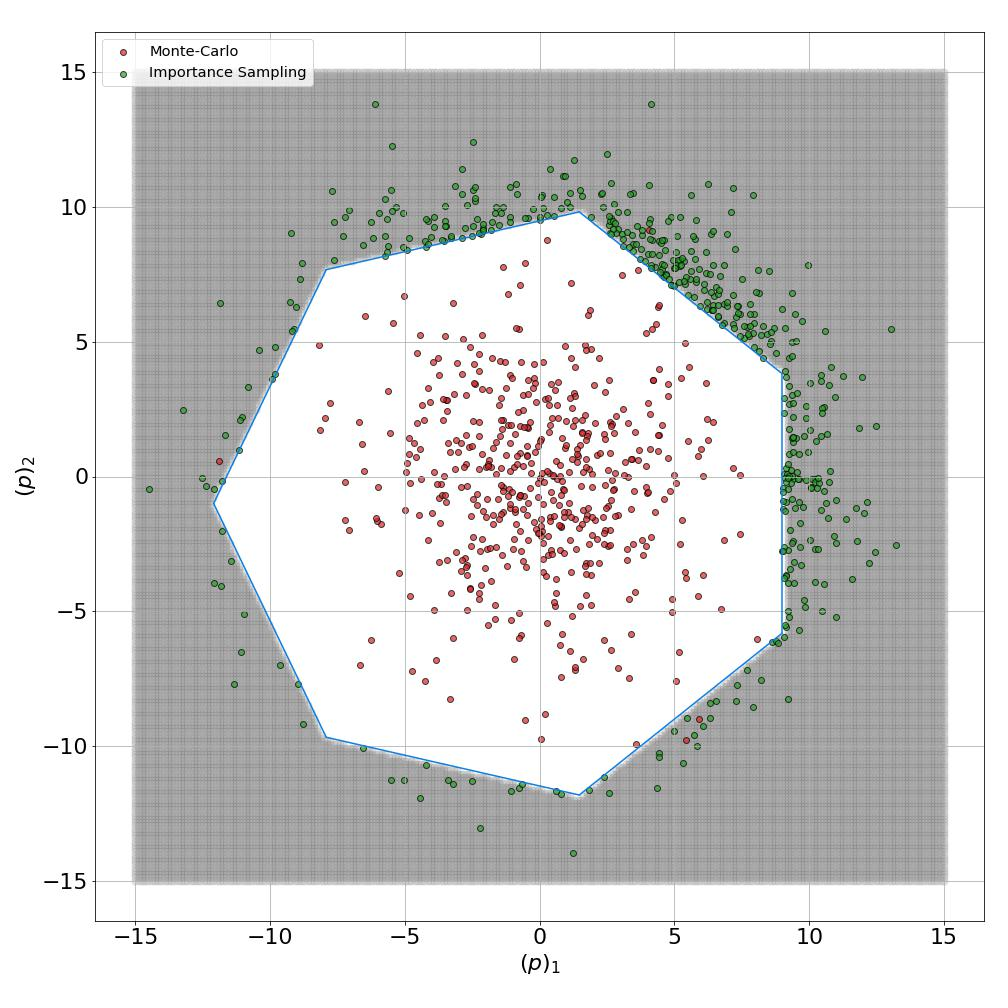
\includegraphics[width=.4\textwidth]{Dissertation/images/dc_stochastic_approx/conditioned_vs_MC (1).jpg}
  \caption{The white area stands for generations that do not exceed operating limits. Power generations that lead to at least one constraint violation are in grey. Two or more reliability constraints are not satisfied in the dark grey area. We mark samples from the nominal distribution and the constructed mixture in red and green, respectively. \cite{lukashevich2021power}.}
  \label{fig:conv_vs_MC}
  
\end{figure}

\subsection{Scenario Approximation with Importance Sampling}

In this section, we present a scenario approximation for the chance-constrained optimal power flow with a set of scenarios generated by the ALOE algorithm~\cite{owen2019importance}. A particular advantage of this approach is that every scenario is generated outside of $\mathcal{P}_{\texttt{in}}$. The latter substantially improves the accuracy and efficiency of the scenario approximation. In particular, we solve the following optimization problem instead of Problem~\eqref{eq:sc-opf}: 
\begin{subequations} 
\label{eq:FinA}
  \begin{equation}
  \min_x \; \textit{cost}(x)\nonumber
  \end{equation}
  \begin{equation}
  \hspace{-20mm}\textit{s. t. }\;\; p^{\min} \le x+\xi^t \le p^{\max}, \; 1\le t \le N\label{eq:FinA-a}
  \end{equation}
  \begin{equation}
   \hspace{11mm} |\theta_i(\xi^t) - \theta_j(\xi^t)| \le {\bar \theta}_{ij}, (i, j)\in \mathcal{E}, \; 1\le t \le N\label{eq:FinA-b}
  \end{equation}
  \begin{equation}
  \hspace{-19mm} x+\xi^t = B \theta(\xi^t), \; 1\le t \le N\label{eq:FinA-c}
  \end{equation}
  \begin{equation}
  \hspace{-50mm} x\in \mathcal{P}_{out} \label{eq:FinA-d}
  \end{equation}
  \begin{equation}
  \hspace{-32mm} \xi^1, \xi^2, \dots, \xi^N\sim D \label{eq:FinA-e},
  \end{equation}
\end{subequations} 
where $D$ is the probability distribution defined by Eq.~\eqref{eq:q_d}. 

Notice, that sampling from distribution $D$ allows to efficiently generate scenarios outside of the polytope $\mathcal{P}_{\texttt{in}}$. However, they follow distribution $D$ instead of $\xi\sim \mathcal{N}(0, \Sigma) \textit{s. t. } \xi\not\in \mathcal{P}_{\texttt{in}}$. As these distributions are close to each other, Theorem~\ref{thm:80} establishes efficient complexity bounds for the scenario approximation with importance sampling. 

\begin{theorem}\label{thm:80}
Let $\bar x_N$ be a unique solution of the Scenario optimization Problem~\eqref{eq:FinA} with $N$ i.i.d. samples follow distribution $D$. Moreover, assume that for any $N$ the assumption \ref{asmp:10} is fulfilled. Then for any $\delta \in (0,1)$ and any~$\eta \in (0, 1/2]$, $\bar x_N$ is also a solution for the chance-constrained optimal power flow Problem~\eqref{eq:JCC-OPF} with probability at least $1-\delta$ if 
\begin{align*}
  N \ge \left\lceil 2M\frac{(1-\pi)\ln \frac{1}{\delta}}{\eta} + 2d + 2d M(1-\pi) \frac{\ln\frac{2M(1-\pi)}{\eta}}{\eta} \right\rceil, 
\end{align*} 
where $d$ is a dimension of the problem and $\pi$ is a probability of a random scenario $\xi$ to belong to $\mathcal{P}_{\texttt{in}}$, $\pi < 1$, and constant $M$ is defined by Theorem~\ref{thm:50}.
\end{theorem}
\begin{proof}
The proof is similar to the one of Theorem~\ref{thm:40}. Application of theorem \ref{thm:50} allows to upper-bound the probability of an event in measure $D$ with respect to its probability in measure $\mathcal{N}(0,\Sigma) \textit{s. t. } \xi\not\in\mathcal{P}_{\texttt{in}}$. 
\end{proof}

We emphasize that Theorem \ref{thm:40} is a key theoretical result demonstrating a potential reduction in the number of samples. The latter is possible if scenarios are from a distribution such that a specific subset of its domain $\mathcal{P}_{\texttt{in}}$ has measure zero. Although, it is not possible to sample directly from such distribution. On the other hand, one can propose a mixture distribution to tackle this problem. In this case, Theorem \ref{thm:50} is a practical statement that allows one to analyze the scenario approximation complexity constructed with scenarios from a mixture distribution.


\section{Empirical Study}\label{sec:emp}
We compare our importance sampling-based approach (referred to as SA-IS) with the classical scenario approximation (SA)~\cite{calafiore2006scenario} over real and simulated test cases.
Empirical results justify our theoretical results: \emph{importance sampling based CC-OPF required much fewer samples to achieve a highly reliable solution than classical scenario approximation.} 

We limit the empirical setting to considering Gaussian distributions and linear feasibility constraints only.
%We omit detailed comparison with other importance sampling strategies \cite{genz2020package,lukashevich2021power,bugallo2017adaptive} when generating scenarios because of the chapter space limitation and for the sake of empirical study clarity. 
A profound discussion on the efficiency of importance samplers is given in~\cite{lukashevich2021power}.
\subsection{Implementation details} We use Python 3.9. and pandapower 2.8.0~\cite{thurner2018pandapower} on MacBook Pro (M1 Max, 64 GB RAM). In the experiments, the computational time for each case does not exceed five minutes, which makes it applicable for the operational practice. Our code is available online on Github~\footnote{https://github.com/vjugor1/IS-SA}. When solving the optimization problem, we use CVX~\cite{diamond2016cvxpy} and GLPK~\cite{GLPK} optimization solvers. 
\begin{figure}[!t]
  \centering
  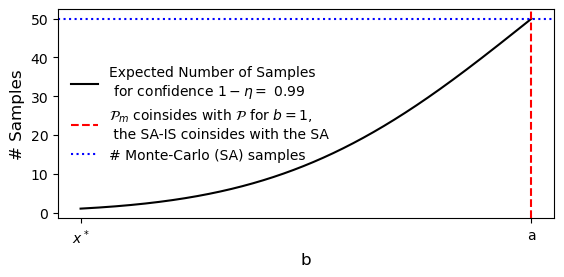
\includegraphics[width=.48\textwidth]{Dissertation/images/dc_stochastic_approx/figure120.png}
  \caption{
  Feasibility of the scenario approximation with importance sampling depending on the size of $\mathcal{P}_{out}= \{x: x\le b\}$, where $a \geq b\geq x^* =a - \Phi^{-1}(1-\eta)$. The more accurate approximation $\mathcal{P}_{out}$ is, the smaller is the number of samples required by the SA-IS algorithm.}
  \label{fig:80}
  
\end{figure}

\subsection{Test Cases and Numerical Results}
\paragraph{Synthetic Example}
For elucidation of the theory, we first study the efficiency of importance sampling based scenarios over a one dimensional test case:
\begin{align*}
  \max\; & x\\
  \textit{s. t. } & \mathbb{P}_\xi(x+\xi \le a) \ge 1-\eta, \xi\sim \mathcal{N}(0,1)
\end{align*}
for $0 < \eta < 1/2$ and a positive constant $a$. In this case, the chance-constrained optimization problem admits an exact solution, $x^* = a - \Phi^{-1}(1-\eta)$. 

The polytopes $\mathcal{P}_{out}$ and $\mathcal{P}_{\texttt{in}}$ are $\{x: x\le x^*\}$ and $\{\xi: \xi \leq \Phi^{-1}(1-\eta)\}$ respectively. To illustrate the role of an approximation $\mathcal{P}_{out}$, $x^* \in \mathcal{P}_{out} \in \mathcal{P}$, we consider different polytopes $\mathcal{P}^b_{m} = \{x: x\le b\}$ and corresponding polytope $\mathcal{P}_{\texttt{in}}^b = \{\xi: \xi \leq a - b\}$, $a - b \le \Phi^{-1}(1-\eta)$.  

Figure~\ref{fig:80} illustrates that the efficiency of sampling improves (i.e., less number of samples needed) as the polytope $\mathcal{P}_{out}$ better approximates $\mathcal{P}_{\texttt{in}}(0)$. Indeed, the probability of a sample from the nominal distribution outside of $\mathcal{P}_{\texttt{in}}^b$ being also outside $\mathcal{P}_{\texttt{in}}$ is proportional to $\Phi(a-b)$, which becomes negligible as $a-b$ decays and leads to a high number of samples. Note, that we reach the standard scenario approximation when $b = a$ and get the best possible approximation for $a-b = \Phi^{-1}(1-\eta)$. 


% \deep{Is the figure plotting a theoretical result..then state the analytical formula that is being depicted}
% \yury{I misunderstand what do you mean guys..}
% \sasha{the formula for this curve is needed, since it is obvously comes from Campi's theory (the plot)}

Our approach crucially relies on a non-conservative/tight approximation of the joint chance-constrained feasible set is crucial for the success of the importance sampling approach, as discussed next for power grid test cases. 

\begin{table*}[t]
    \centering
    \adjustbox{width=.9\textwidth}{
        \begin{tabular}{lrrll|rll|l}
        \toprule
           Case &  $\eta$ &  SA No &  SA Cost &   SA $(\mathbb{P}_N)$ &  IS-SA No & IS-SA Cost & IS-SA $(\mathbb{P}_N)$ & DC-OPF Cost \\
        \midrule
         grid30 &    0.05 &    160 & 5.89e+03 & 9.82e-01$\pm$7.09e-03 &        \textbf{60} &   5.87e+03 &  9.80e-01$\pm$8.86e-03 &    5.67e+03 \\
         grid57 &    0.05 &    210 & 2.52e+04 & 9.78e-01$\pm$8.95e-03 &       \textbf{160} &   2.52e+04 &  9.89e-01$\pm$7.71e-03 &    2.50e+04 \\
        grid118 &    0.05 &   1300 & 8.72e+04 & 9.68e-01$\pm$4.18e-03 &      \textbf{1050} &   8.72e+04 &  9.68e-01$\pm$4.16e-03 &    8.48e+04 \\
        grid300 &    0.05 &   1550 & 4.72e+05 & 9.63e-01$\pm$4.36e-03 &      \textbf{1250} &   4.72e+05 &  9.62e-01$\pm$3.97e-03 &    4.71e+05 \\
        \midrule
         grid30 &    0.01 &    800 & 5.94e+03 & 9.96e-01$\pm$1.83e-03 &       \textbf{300} &   5.96e+03 &  9.99e-01$\pm$6.57e-04 &    5.67e+03 \\
         grid57 &    0.01 &   1300 & 2.52e+04 & 9.96e-01$\pm$1.55e-03 &       \textbf{300} &   2.53e+04 &  9.97e-01$\pm$1.88e-03 &    2.50e+04 \\
        grid118 &    0.01 &   6000 & 8.74e+04 & 9.93e-01$\pm$1.16e-03 &      \textbf{3600} &   8.74e+04 &  9.94e-01$\pm$9.11e-04 &    8.48e+04 \\
        grid300 &    0.01 &   9000 & 4.72e+05 & 9.93e-01$\pm$8.42e-04 &      \textbf{4500} &   4.72e+05 &  9.92e-01$\pm$9.53e-04 &    4.71e+05 \\
        \bottomrule
        \end{tabular}
    }
    \caption{Number of SA-IS and SA samples required to reach reliability level $1-\hat{\delta} = 0.99$ in CC-OPF with confidence threshold $1-\eta$. The number of scenarios required for target reliability were obtained empirically, iterating over a predefined grid for $N$ with the step of $10$.
    The confidence threshold $1-\eta$ is estimated using Monte Carlo samples (out of sample) and empirical reliability is computed by averaging over $L=100$ independent CC-OPF problem instances as stated in Algorithm~\ref{alg:estimate_delta}. The costs of solutions obtained are depicted alongside with the corresponding costs of deterministic DC-OPF solution. It is clear that SA-IS requires much less samples compared to SA, while maintaning the same reliability of the solution.}
    
    \label{tab:summary_results}
\end{table*}


\paragraph{Power grid test cases}
We address the scenario-based chance-constrained optimal power flow problem (CC-OPF) under Gaussian fluctuations in four different test cases (IEEE 30, IEEE 57, IEEE 118 and IEEE 300 bus systems with 30, 57, 118 and 300 buses/nodes, respectively). For all considered cases, we assume the power generation and consumption level fluctuate with the standard deviation of 0.07 of its nominal value. 

To demonstrate the practical benefits of importance sampling (SA-IS) versus standard scenario approximation (SA), we compare their respective number of samples $N$ needed to solve CC-OPF for different test cases, given prescribed $\eta,\delta$. As stated in theorems in Section \ref{sec:algo}, $1-\eta$ is the required \emph{confidence threshold} for constraint feasibility (of Joint Chance Constraint) by a solution, while $1-\delta$ is the required reliability of the Scenario Approximation's solution obtained.


We consider the setting of fixed confidence threshold $1-\eta$ and $N$, the number of samples used in CC-OPF (with SA-IS or SA), and determine their effect on empirical reliability $1-\hat{\delta}$ using Algorithm \ref{alg:estimate_delta}. In Algorithm \ref{alg:estimate_delta}, we independently form $L=100$ different scenario approximation problems, each with $N$ scenarios constructed using SA or SA-IS. We thus obtain $L$ different solutions $(x^*_N)_l, ~ l=1, \dots, L$. Using separately generated $10^4$ Monte Carlo samples of uncertainty for each $(x^*_N)_l$, we estimate each solution's probability of constraint satisfaction $(\hat{\mathbb{P}}_N)_l$. The estimated reliability $1-\hat{\delta}$ is then given by the fraction of $L$ $(x^*_N)_l$ solutions with $(\hat{\mathbb{P}}_N)_l \geq 1 - \eta$. 

\begin{algorithm}[ht]
\SetKwInOut{Input}{input}
\SetKwRepeat{Do}{do}{while}
% \SetKwInOut{Output}{output}
\caption{Reliability $1-\hat{\delta}$ -- an empirical estimate}\label{alg:estimate_delta}
\Input{$L$ -- number of trials, DC-OPF problem parameters, $\eta$ -- confidence level, $N_0$ -- initial size of scenario approximation, $N_{\max}$ -- maximal size of scenario approximation}
$N \gets N_0$\;
$\hat{ \boldsymbol \delta}$ -- storage for $\hat{\delta}_N$\;
\Do{$N \leq N_{\max}$}
{
     $C_N \gets 0$ -- feasibility counter\;
     $l \gets 1$\;
    \Do{$l \leq L$}{
        Obtain $(x^*_N)_l$ -- scenario approximation with $N$ samples (using SA-IS or SA) \;
        Estimate constraint satisfaction probability $(\hat{\mathbb{P}}_N)_l$ using Monte Carlo samples.\; \label{alg:estimate_delta:phat_N_l}\;
        \uIf{$(\hat{\mathbb{P}}_N)_l \geq 1 - \eta$}{
            $C_N \gets C_N +1$
        }
        }
    $1-\hat{\delta}_N \gets C_N / L$ -- fraction of trials turned out to be feasible \;
    Append $\hat{\delta}_N$ to $\hat{ \boldsymbol \delta}$ \;
    $n  \gets n + N_{\max}/ 10$\;
}
\Return $\hat{ \boldsymbol \delta}$
\end{algorithm}

% \begin{algorithm}[ht]
% \caption{Reliability $1-\hat{\delta}$ -- an empirical estimate}\label{alg:estimate_delta}
% \begin{algorithmic}
% \Require $L$ -- number of trials, DC-OPF problem parameters, $\eta$ -- confidence level, $N_0$ -- initial size of scenario approximation, $N_{\max}$ -- maximal size of scenario approximation
% \State $N \gets N_0$
% \State $\hat{ \boldsymbol \delta}$ -- storage for $\hat{\delta}_N$
% \While{$N \leq N_{\max}$}
%     \State $C_N \gets 0$ -- feasibility counter
%     \State $l \gets 1$
%     \While{$l \leq L$}
%         \State Obtain $(x^*_N)_l$ -- scenario approximation with $N$ samples (using SA-IS or SA)
%         \State Estimate constraint satisfaction probability $(\hat{\mathbb{P}}_N)_l$ using Monte Carlo samples. \label{alg:estimate_delta:phat_N_l}
%         \If{$(\hat{\mathbb{P}}_N)_l \geq 1 - \eta$}
%             $C_N \gets C_N +1$
%         \EndIf
%     \EndWhile
%     \State $1-\hat{\delta}_N \gets C_N / L$ -- fraction of trials turned out to be feasible
%     \State Append $\hat{\delta}_N$ to $\hat{ \boldsymbol \delta}$
%     \State $n  \gets n + N_{\max}/ 10$
% \EndWhile
% \State \Return $\hat{ \boldsymbol \delta}$
% \end{algorithmic}

% \end{algorithm}

Table~\ref{tab:summary_results} summarizes the number of samples needed using SA and SA-IS to ensure an empirical reliability of $0.99$, for two confidence thresholds $1-\eta$ ($0.95$ and $0.99$). Our experiments show that SA-IS requires much fewer samples to provide a reliable CC-OPF feasible solution while maintaining the same cost for each test case compared to CC-OPF with SA. The improvement in the number of scenarios is bigger for the higher confidence threshold value ($1-\eta=0.99$).

We illustrate the dependence between empirical reliability $1-\hat{\delta}$ and $N$ over a range of values for the IEEE 118 bus system in Fig.~ \ref{fig:ieee118reliability}. Here, we keep a confidence threshold of joint chance constraint feasibility $1-\eta =0.99$. In addition to SA-IS and SA, we also consider an intermediate setting - Scenario Approximation with Polygon-Set (SA-O), as described in Eq.~\eqref{eq:Fin}. 

Compared to SA, SA-O includes the inner approximation constraints $x \in \mathcal{P}_{out}$. However, unlike SA-IS, SA-O does not involve importance sampling-based samples. It is clear from Fig.~\ref{fig:ieee118reliability} that at all values of $N$, SA-IS's reliability $1-\hat{\delta}$ is much higher than that of SA or SA-O. In fact, for $3500\leq N \leq 4000$, the SA-IS is around ten times more reliable than SA. As a result, the solution of SA-IS also becomes conservative faster (highlighted by the decrease in slope at higher reliability). On the other hand, SA and SA-O have almost similar reliability, which follows from Theorem \ref{thm:20}. 

Finally, for the same $L$ optimization instances used for Fig.~\ref{fig:ieee118reliability}, we present box-plots for the spread of $(\hat{\mathbb{P}}_N)_l$ for different $N$, in Fig.~\ref{fig:ieee118conservatism}. Here, $(\hat{\mathbb{P}}_N)_l$ is the probability of constraint satisfaction, empirically computed using $10^4$ Monte Carlo separately generated samples of Algorithm \ref{alg:estimate_delta}, see Eq.~\ref{alg:estimate_delta:phat_N_l}. Note that SA-IS reaches a higher reliability level ($1-\hat{\delta}$) at a fewer number of samples $N$, observed when almost all of the box is above the $1-\eta$ threshold. The boxplots also indicate that the variance in the obtained solution's chance-constraint feasibility reduces faster for SA-IS, noted by thinner boxplots and lack of outliers, compared to SA and SA-O.

\begin{figure*}[hbt]

\begin{subfigure}{.48\textwidth}
  \centering
  % include first image
  \hspace{-4mm}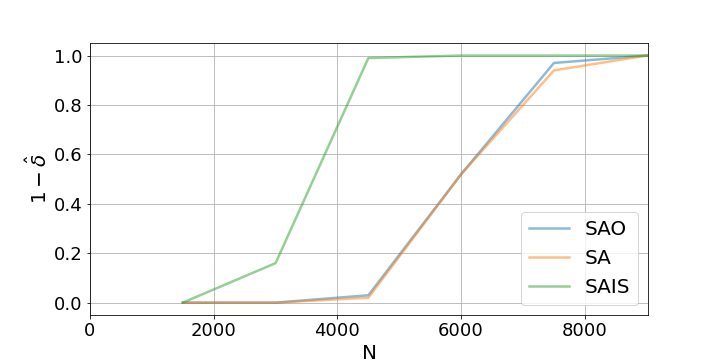
\includegraphics[width=0.9\linewidth]{Dissertation/images/dc_stochastic_approx/case300/1_beta_N_12000_eta_001.png}~~~~~~\hfill
  \caption{Empirical reliability ($1-\hat{\delta}$) versus number of samples in \\CC-OPF ($N$) for IEEE 300 bus system.}
  \label{fig:ieee300reliability}
\end{subfigure}
\begin{subfigure}{.48\textwidth}
  \centering
  % include second image
  \hspace{-8mm}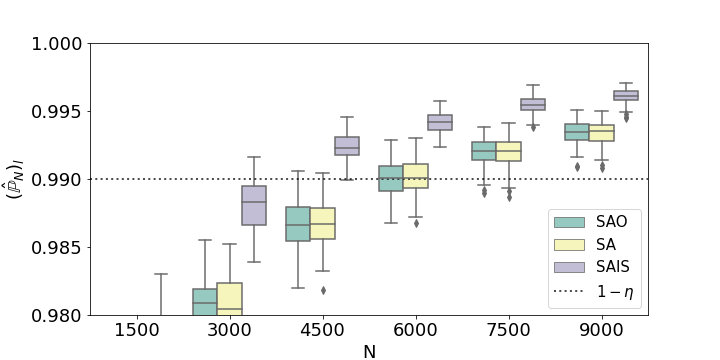
\includegraphics[width=0.9\linewidth]{Dissertation/images/dc_stochastic_approx/case300/boxplot_J_N_9000_eta_001.png}
  \caption{Spread of probability of constraint feasibility ($(\hat{\mathbb{P}}_N)_l$) \\versus number of samples in CC-OPF ($N$) for IEEE 300 bus system.}
  \label{fig:ieee300conservatism}
\end{subfigure}

\begin{subfigure}{.48\textwidth}
  \centering
  % include first image
  \hspace{-4mm}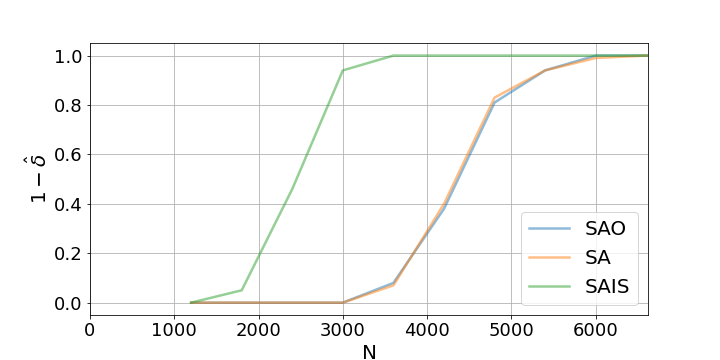
\includegraphics[width=0.9\linewidth]{Dissertation/images/dc_stochastic_approx/ieee118/1_beta_N_7800_eta_001.png}~~~~~~\hfill
  \caption{Empirical reliability ($1-\hat{\delta}$) versus number of samples in \\CC-OPF ($N$) for IEEE 118 bus system.}
  \label{fig:ieee118reliability}
\end{subfigure}
\begin{subfigure}{.48\textwidth}
  \centering
  % include second image
  \hspace{-8mm}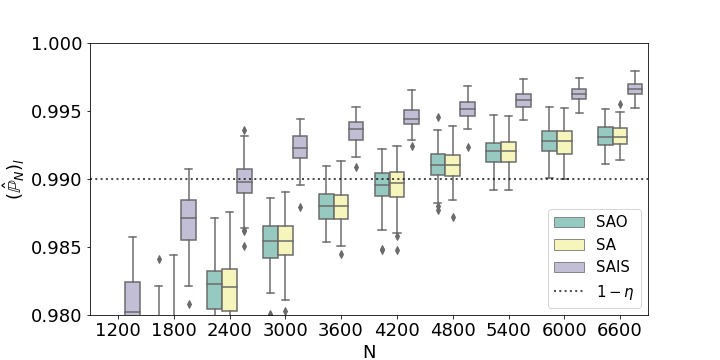
\includegraphics[width=0.9\linewidth]{Dissertation/images/dc_stochastic_approx/ieee118/boxplot_J_N_6600_eta_001.png}
  \caption{Spread of probability of constraint feasibility ($(\hat{\mathbb{P}}_N)_l$) \\versus number of samples in CC-OPF ($N$) for IEEE 118 bus system.}
  \label{fig:ieee118conservatism}
\end{subfigure}
% \begin{subfigure}{.48\textwidth}
%   \centering
%   % include second image
%   \hspace{-1mm}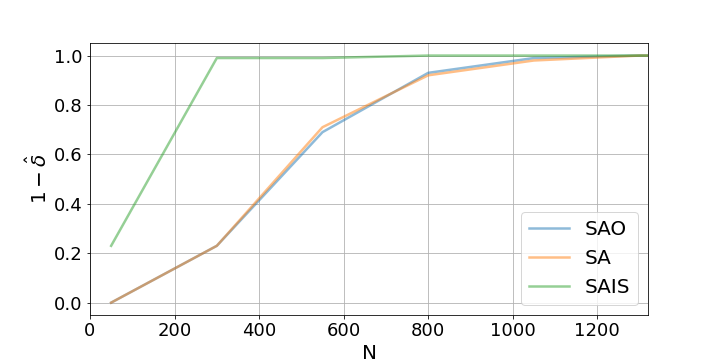
\includegraphics[width=0.9\linewidth]{Dissertation/images/dc_stochastic_approx/ieee57/1_beta_N_2300_eta_001.png}~~~~~~\hfill
%   \caption{Empirical reliability ($1-\hat{\delta}$) versus number of samples in \\CC-OPF ($N$) for IEEE 57 bus system.}
%   \label{fig:ieee57conservatism}
% \end{subfigure}
% \begin{subfigure}{.48\textwidth}
%   \centering
%   % include first image
%   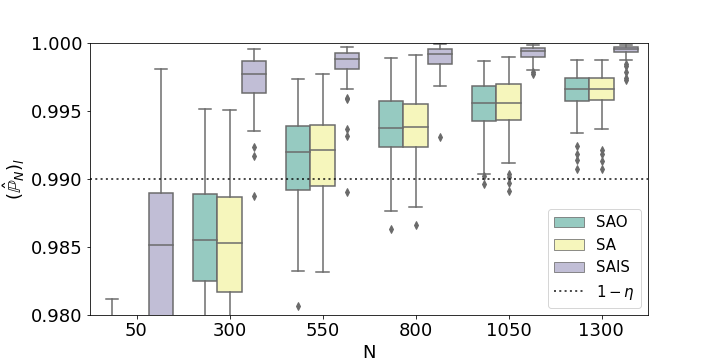
\includegraphics[width=0.9\linewidth]{Dissertation/images/dc_stochastic_approx/ieee57/boxplot_J_N_1300_eta_001.png}~~~~~~\hfill
%   \caption{Spread of probability of constraint feasibility ($(\hat{\mathbb{P}}_N)_l$) \\versus number of samples in CC-OPF ($N$) for IEEE 57 bus system.}
%   \label{fig:ieee57reliability}
% \end{subfigure}
% \begin{subfigure}{.48\textwidth}
%   \centering
%   % include second image
%   \hspace{-1mm}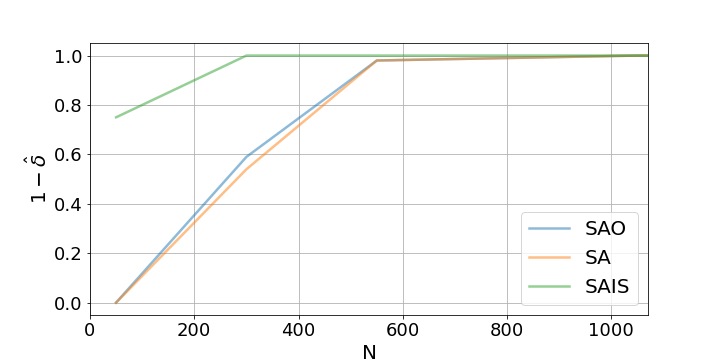
\includegraphics[width=0.9\linewidth]{Dissertation/images/dc_stochastic_approx/ieee30/1_beta_N_2300_eta_001.png}~~~~~~\hfill
%   \caption{Empirical reliability ($1-\hat{\delta}$) versus number of samples in \\CC-OPF ($N$) for IEEE 30 bus system.}
%   \label{fig:ieee30conservatism}
% \end{subfigure}

% \begin{subfigure}{.48\textwidth}
%   \centering
%   % include first image
% ~~~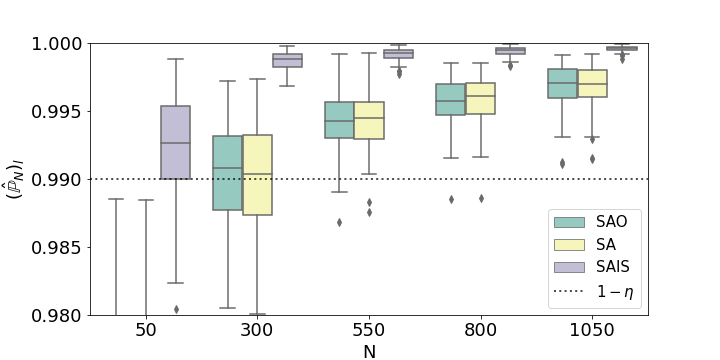
\includegraphics[width=0.9\linewidth]{Dissertation/images/dc_stochastic_approx/ieee30/boxplot_J_N_1050_eta_001.png}\hfill
%   \caption{Spread of probability of constraint feasibility ($(\hat{\mathbb{P}}_N)_l$) \\versus number of samples in CC-OPF ($N$) for IEEE 30 bus system.}
%   \label{fig:ieee30reliability}
% \end{subfigure}

\caption{(a, c) Empirical reliability ($1-\hat{\delta}$) and (b, d) The spread of constraint feasibility $(\hat{\mathbb{P}}_N)_l$ for CC-OPF ($1-\eta =.99$) in IEEE 300 bus (IEEE 118 bus, resp.) system. The three cases correspond to samples in CC-OPF being drawn by SA, SA-IS and SA-O. The empirical estimates are computed with $L = 100$ optimization instances (for $1-\hat{\delta}$), and $N_{MC}=10^4$ Monte-Carlo samples for each instance to determine constraint validation (for box-plot of $(\hat{\mathbb{P}}_N)_l$), as described in Algorithm~\ref{alg:estimate_delta}. 
Colored boxes stands for the 25\% -- 75\% interquantile range (IQR). Diamonds shows samples outside of the $\pm 1.5*\text{IQR}$. 
Note that both in reliability, and the IRQ of constraint feasibility, SA-IS requires much less number of samples compared to SA or~SA-O.}
\label{fig:ieee118}
\end{figure*}

Finally, we address the question if the total computational time for SA-IS is better than for classical SA. First, we address the amount of time required to generate samples for classical Monte-Carlo SA, and those for IS-SA using Importance Sampling technique. Next, we analyze how to much time totally is required to obtain $1-\hat{\delta}=0.99$-reliable solution. For such experiment we consider generating samples for IEEE-30 power system. 

In order to compare preprocessing step, i.e., sampling generation step, we generate $N=50, 150, 250, 350, 450$ samples with ALOE, and the same amount of samples from multivariate normal distribution. For each $N$ we repeat generation 15 times to obtain statistics on execution time. Similarly, with the same strategy we generate the samples for each $N$ and solve the scenario approximation and collect execution time, repeating for 15 times. 
The execution time of the preprocessing step comparison is visualized in Figure \ref{fig:profile_generate_samples}. From here one can observe that ALOE is a more time consuming procedure. However, one can observe that the time required to solve scenario approximations together with preprocessing does not differ significantly for IS-SA and SA -- see Figure \ref{fig:profile_scenario_approx}. The latter figure also shows that the computational time required to obtain the same reliability level is five times less for SA-IS (the number of samples are taken from Table \ref{tab:summary_results}, case IEEE-30, $\eta=0.05$.)

\begin{figure*}[hbt]

\begin{subfigure}{.48\textwidth}
  \centering
  % include first image
  \hspace{-4mm}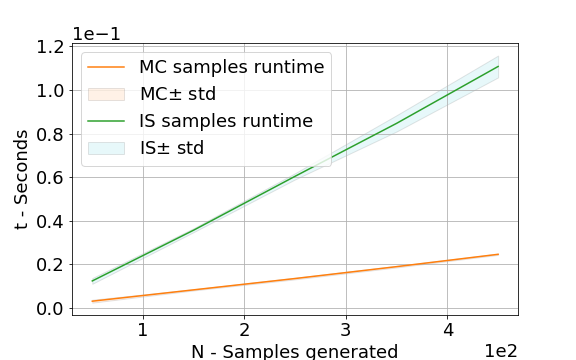
\includegraphics[width=0.9\linewidth]{Dissertation/images/dc_stochastic_approx/profiling_samplig.png}~~~~~~\hfill
  \caption{Computational time required to complete the pre-processing step, that is sample required scenarios.}
  \label{fig:profile_generate_samples}
\end{subfigure}
\begin{subfigure}{.48\textwidth}
  \centering
  % include second image
  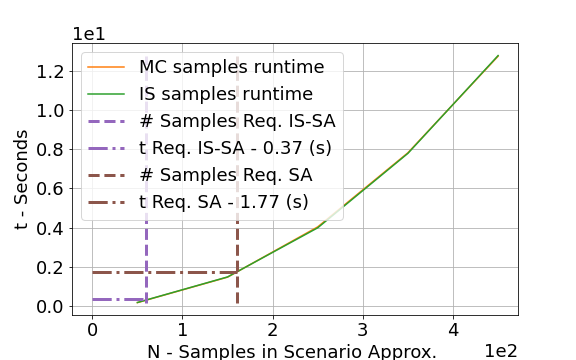
\includegraphics[width=0.9\linewidth]{Dissertation/images/dc_stochastic_approx/profiling_approx_sol.png}
  \caption{Computational time required to prepare samples and solve scenario approximations formed for different $N$. }
  \label{fig:profile_scenario_approx}
\end{subfigure}

\caption{Computational time required to complete prepocessing step \ref{fig:profile_generate_samples} and solve corresponding scenario approximations \ref{fig:profile_scenario_approx} for IEEE-30 case. On the right Figure, vertical dashed lines indicate number of samples that are sufficient to reach $1-\hat{\delta}=0.99$ reliability level for $\eta=0.05$, see Table \ref{tab:summary_results}. Horizontal dot-dashed lines demonstrate the amount of time spent on average over 15 runs.}
\label{fig:profiling}

\end{figure*}


\section{Conclusion}
\label{sec:conclusion}
In this chapter, we investigated the scenario approximation for the chance-constrained optimal power flow. We showed that the importance sampling technique used for scenario generation leads to a better accuracy. Moreover, the numerical complexity is much lower in theory and practice for stochastic OPF. 

The theoretical study indicates benefit from using violative samples. The results are presented and proven alongside with numerical experiments that indicate significant reduction of sample size in scenario approximation required to reach a high reliability level. Finally, the approach can be extended to automated real-time control of bulk power systems. 
\chapter{A-Priori Reduction of Scenario Approximation for Dynamic DC-OPF}
This chapter is based on the publication of the dissertation author: \fullcite{lukashevich2023importance}. 
\label{chap:apriori_stochastic_approx}

\section{Introduction}
\label{sec:introduction}
\vspace{-1mm}
Integrating renewable energy sources aligns with the United Nations' sustainable development goals, promoting affordable and clean energy while enhancing energy security and resilience. Unfortunately, RES introduces significant uncertainty in power systems generation, posing substantial challenges to grid optimization and control policies.

The Optimal Power Flow (OPF) \cite{stott2012optimal} is a key optimization problem that aims to achieve economically optimal generation while adhering to grid security and power balance constraints. To account for generation uncertainty, the Joint Chance-Constrained (JCC) extension considers an unknown joint distribution of renewable energy sources \cite{geng2019data, bienstock2014chance}. An alternative robust optimization approach assumes bounded uncertainty and offers a more conservative solution in practice \cite{ben2002robust, ding2016adjustable}.
%
The discrete-time dynamic chance-constrained OPF problem \cite{lou2019multi, capitanescu2007improving, monticelli1987security} models optimal generation set-points for sequential timestamps, temporarily binding generators' power outputs through ramp-up and ramp-down constraints. These constraints model the limit of the rate of change of the power output, as significant immediate changes are not feasible for some generators \cite{frangioni2008solving}. Automatic Generation Control (AGC) is widely used for fast and efficient power dispatch in bulk power systems \cite{xu2017real}.



While the chance-constrained extension enhances flexibility in modeling uncertainty, solving it for an arbitrary distribution and/or jointly for all technical limits becomes computationally infeasible~\cite{nemirovski2012safe, jia2021iterative}. To overcome this, Data-Driven (DD) approximations such as Scenario Approximation (SA) \cite{calafiore2006scenario} and Sample Average Approximation (SAA)~\cite{ahmed2008solving} have proven successful.

Unfortunately, data-driven (scenario) approaches are often computationally prohibitive when a higher accuracy approximation is required. The latter motivates extensive scenario reduction studies.

Scenario reduction methods can be divided into two categories: a-posteriori and a-priori methods. In the first case, one needs to solve SA of the initial JCC problem many times, iteratively identifying reducible scenarios \cite{campi2011sampling, geng2019data}. In contrast, a-priori scenario reduction methods reduce the number of scenarios before solving SA, thus enhancing computational efficiency. A-priori scenario reduction methods were pioneered in~\cite{dupavcova2003scenario, dupavcova1990stability} and further refined in~\cite{heitsch2003scenario}. These methods use probability metrics like the Wasserstein distance to decide which scenarios to drop. Alternatively, some methods replace the initial set with a smaller, more representative set through clustering or similar approaches \cite{rujeerapaiboon2022scenario, keutchayan2023problem, liang2020scenario}.


The key difference between a-posteriori and a-priori reductions lies in the theoretical guarantees for SA solution feasibility for the original JCC problem. To the best of our knowledge, such guarantees are limited in the literature for a-priori methods. To fill this gap, we propose A-priori Reduced Scenario Approximation (AR-SA) - an approach for a-priori sample reduction methods linked with a data-driven Scenario Approximation (SA). The resulting SA requires significantly fewer samples to produce a reliable solution for JCC dynamic DC optimal power flow  and prove theoretical guarantees for such reduction methods in terms of feasibility for JCC DC-OPF.

The contributions of this chapter are as follows. First, we analytically define a-priori conditions that determine sample redundancy for JCC dynamic optimal power flow with AGC and provide theoretical support for these conditions. Second, we analyze dataset size requirements for AR-SA data-driven approximation based on the reduced dataset, taking into account solution reliability. Third, we compare the performance of the AR-SA approach with SA constructed on reduced scenario sets. The scenario reduction methods used are Fast Forward (FF) \cite{dupavcova2003scenario}, Simultaneous Backward (SB) \cite{heitsch2003scenario}, and $K$-Means \cite{keutchayan2023problem}. We use standard SA as a baseline.For proposed AR-SA we observe nearly a twofold improvement in data efficiency compared to other scenario reduction techniques. We summarize the chapter's workflow in Figure \ref{fig:workflow}. We compare the performance of AR-SA with other reduction techniques such as Fast Forward, Simultaneous Backward, and K-Means methods on Grid6-WW, Washington-14, and IEEE-30 grids.

\begin{figure}
    \centering
    \hspace{-2mm}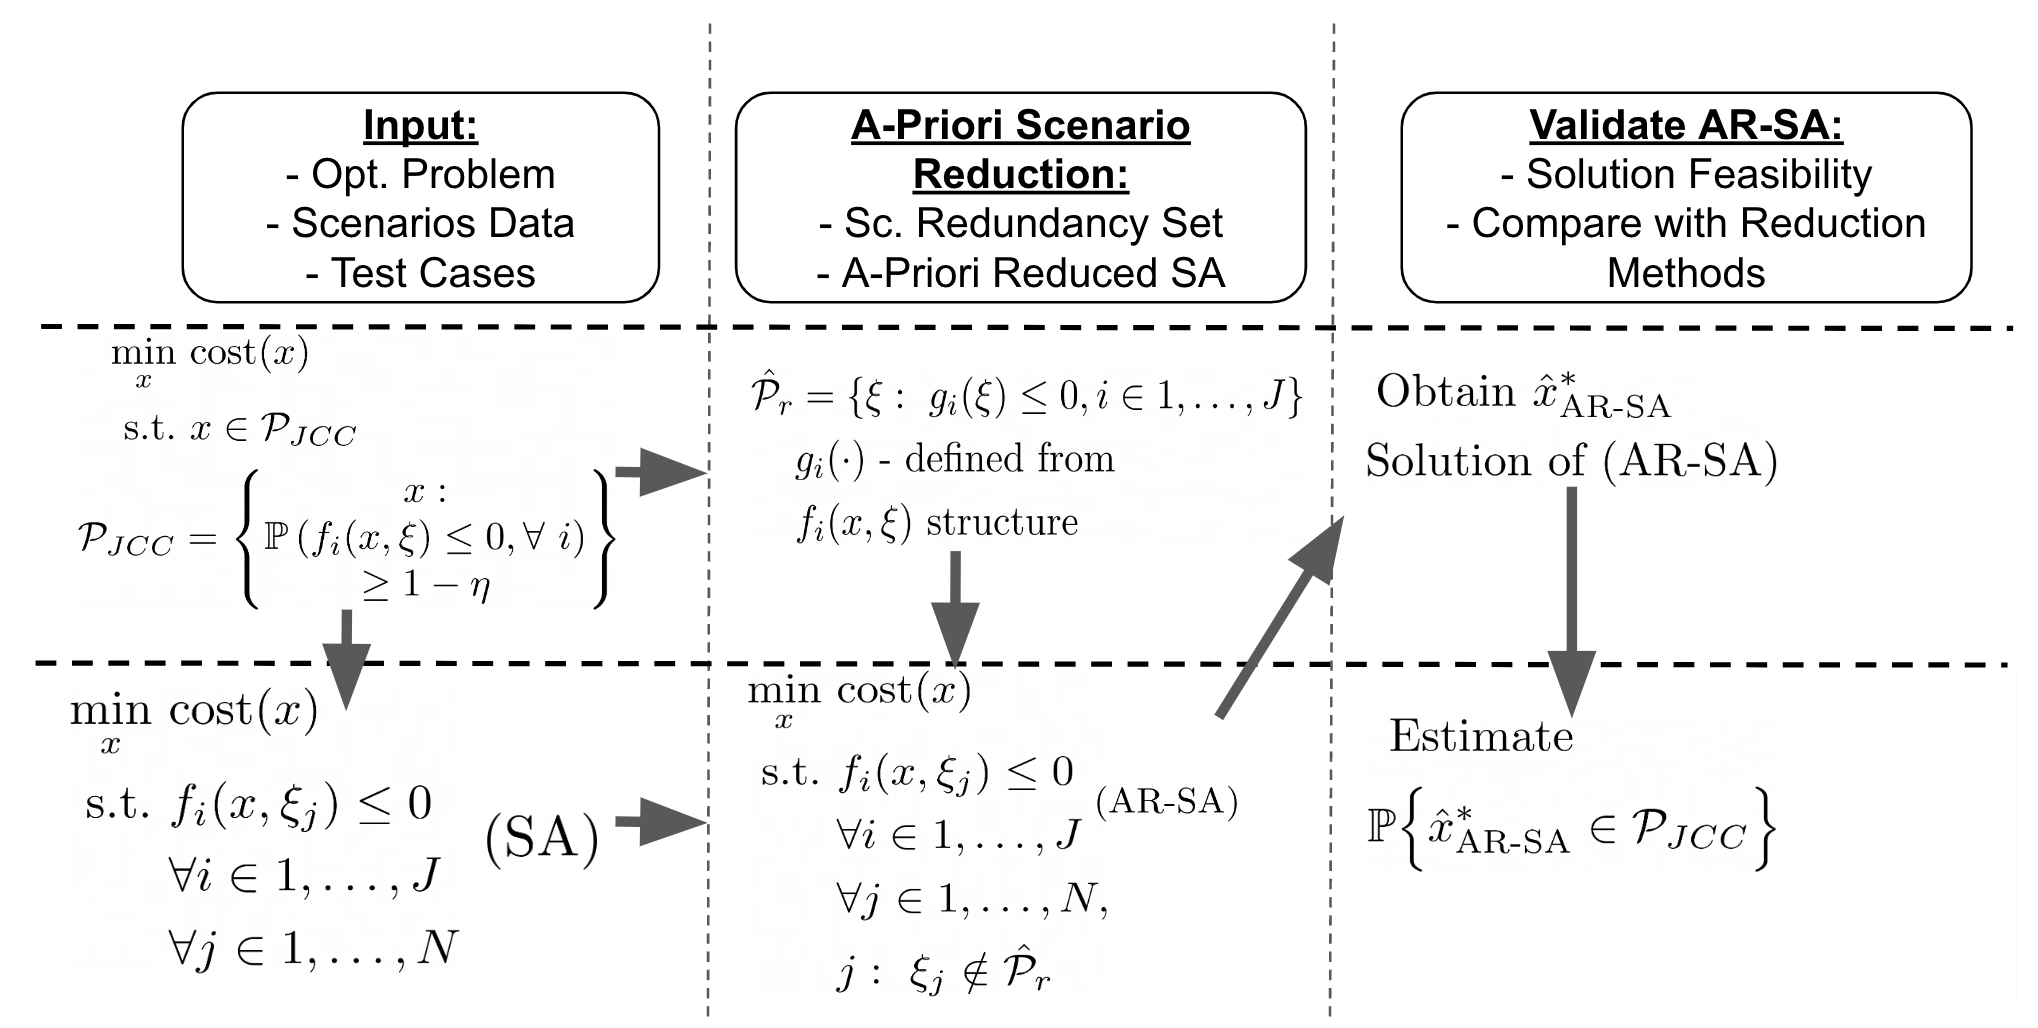
\includegraphics[width=1.\textwidth]{Dissertation/images/dynamic//scheme.png}
    \caption{AR-SA workflow.}
    \label{fig:workflow}
    \vspace{-1mm}
\end{figure}

The rest of this chapter is organized as follows. Section~\ref{sec:setup} provides background and problem setup of the multi-stage high-voltage optimal power flow. Section~\ref{sec:chancecontrol} discusses the setup of the multi-step high-voltage OPF with automated generation control. Section~\ref{sec:chancecontrol} formulates the chance-constrained problem under consideration. Section~\ref{sec:apriori} presents the sketch of the a-priori sample reduction approach, formalizes, and proves its validity. Furthermore, we prove that AR-SA (reduced data-driven approximation) theoretically requires fewer data samples to produce a reliable solution than classical SA. Section~\ref{sec:emp} compares AR-SA with classical Monte Carlo-based SA and other scenario reduction methods such as Fast Forward (FF), Simultaneous Backward (SB), and the clustering K-Means method.

Finally, the conclusion is in Section \ref{sec:conclusion}.
%\vspace{-4mm}
\section{Background and Problem Setup}\label{sec:setup}
\subsection{DC Optimal Power Flow}
%\vspace{-1mm}
The high-voltage DC model is a widely used load flow model in power systems. 

Let $G = (V, E)$ be a power system graph with the set of $n$ nodes (buses) $V$ and the set of $m$ lines (edges) $E$; 
%
$p \in \mathbb{R}^{n_g}$, $p_d \in \mathbb{R}^{n_d}$, and $\theta\in\mathbb{R}^{n}$ be vectors representing power generations, demands, and phase angles, respectively. 

The system is balanced so the sum of all power injections is zero, $\sum_{i \in V} p^i = \sum_{i \in V} p^i_d$.
For clarity we designate one bus as the slack bus, with its phase angle set as $\theta_s = 0$. 
The components of admittance matrix $B$, $B \in \mathbb{R}^{n \times n}$, denoted as $B^{ij}$, are non-zero if there is a line between buses $i$ and $j$. For each node $i$, $B^{ii}$ is defined as the negative sum of the off-diagonal elements $B^{ij}$ with $j \neq i$. 
The DC power flow equations, security and constraints for $i \in V, (i,j)\in E$ are:% expressed as follows:
\vspace{-3mm}
\begin{gather*}
p-p_{d} = B \theta, \!\sum_{i=1}^{n_g} p^i = \!\!\!\sum_{i=1}^{n_d} p^i_d, 
\underline{p}^i_g \leq p^i_g \leq \overline{p}^i, |\theta^i - \theta^j| \leq \bar{\theta}^{ij}
\vspace{-2mm}
\end{gather*}
These equations represent the DC power flow and enforce generation and reliability constraints. 

% \end{comment}
The DC Optimal Power Flow (DC-OPF) feasibility set is linear, determined by voltage phases and power generation within grid topology, line characteristics (admittance matrix), and power demand \cite{wood2013power} (Chapter 4.1.4). The objective is to find an economically optimal active power generation profile across available generators while adhering to technical limits and system demand, which define rules and technical limits on power transfer throughout the system.
The feasibility set of DC-OPF can be reformulated as a polytope $P = {p: Wp \leq b}$ in the vector space of active power generations $p \in \mathbb{R}^{n_g}$, where $W \in \mathbb{R}^{J \times n_g}$ and $b \in \mathbb{R}^J$. Here, $n_g$ denotes the number of controllable generators, and $J$ represents the number of constraints \cite{lukashevich2021importance}, \cite{ lukashevich2021power, owen2019importance}. Reliability constraints are violated when the power generation vector $p$ falls outside the polytope $P$.

Solving DC-OPF consists of finding the power flow by minimizing a convex cost of power generation $c(p_g)$ subject to the constraints defined by $P$. 
\vspace{-1mm}
\subsection{Source of uncertainty and AGC}
\label{sec:fluctuations}
\vspace{-2mm}

The fluctuations affect the power balance in the system and are typically managed through primary and secondary control \cite{machowski2020power}. In this chapter, we consider linear Automatic Generation Control (AGC). The AGC recourse adjusts the generation to a new setpoint $p^{t+1} = p^t + \alpha \xi^t$ \cite{roald2017chance,baros2021examining,mezghani2020stochastic} with $p^t \in \mathbb{R}^{n_g}$, $\alpha \in \mathbb{R}^{n_g}$, and $\xi^t \in \mathbb{R}$ representing the \emph{total} demand-generation imbalance.

The participation factors $\alpha$ for secondary control can slightly vary, enabling long-term grid stability and fast control~\cite{machowski2020power}. 


The total system imbalance $\xi^{t}$ is a sum of power fluctuations caused by an intermittency of renewable generation, demand instability, and intra-day electricity trading. More specifically, if a power system has nodes $\mathcal{B}$, $\xi^t = \sum_{b \in \mathcal{B}} (\xi_b^d)^t - (\xi_b^g)^t$, where $(\xi_b^d)^t$ and $(\xi_b^g)^t$ are random variables that model fluctuations at bus $b$, at time stamp $t$ in demand and generation, respectively. Depending on the source, these random variables follow various distributions. For example, if a bus $b$ contains a PV generator, then $(\xi_b^g)^t$ follows beta distribution \cite{wang2010probabilistic}, if there is a wind farm, wind speed distribution is Weibull, however, power output can be vary from turbine to turbine \cite{dhople2012framework}. Nevertheless, $\xi^t$ is a sum of random variables and, due to the Lyapunov or Lindeberg-Feller Central Limit Theorem \cite{scholz2011central}, follows Gaussian distribution \cite{rouaud2013probability, draper2021practical}. We also checked the validity of this assumption by applying Shapiro-Wilk normality test \cite{shapiro1965analysis} on time series of load-renewable generation imbalance estimated from RTS-GLMC data \cite{barrows2019ieee}. The latter project incorporates time series for demand, hydro, rooftop PV, PV, wind farms generations. The Shapiro-Wilk testing revealed that, on significance level of $\alpha=0.05$, the $H_0$ hypothesis (the generation-demand imbalance is distributed normally) is rejected only for August and November. The testing results are monthly-wise and presented in Table \ref{tab:shapiro-wilk}. Thus, the assumption that $\xi^t$ is Gaussian is valid. We further consider stacked temporal uncertainty vector $\xi = (\xi^1, \dots, \xi^T) \sim \mathcal{\mu, \Sigma}$ and $\Sigma$ here models temporal correlations.

Given the samples $X_1, \dots, X_{n_s}$, the Shapiro-Wilk test uses the following $H_0$ hypothesis: the samples are drawn from a normal distribution $\mathcal{N}(\mu_s, \sigma^2_s)$. The alternative $H_1$ is that the population is not normal. This test is one-tailed. The following statistic is applied: $W_{\textup{S-W}} = \frac{\left( \sum_{i=1}^{n_s} a_i X_{(i)} \right)^2}{\sum_{i=1}^{n_s} \left( X_i - \bar{X}\right)^2}$, where $\bar{X} = \frac{1}{n_s} \sum_{i=1}^{n_s} X_i$ and $X_{(i)}$ -- $i^{\textup{th}}$ order statistic. The coefficients $a_i$ are defined using samples $Z_1, \dots Z_{n_s} \sim \mathcal{N}(0, 1)$. Denote $V$ as the covariance matrix of the standard normal samples: $V_{ij} = \mathbb{E}\left[ (Z_{(i)} - m_i)(Z_{(j)} - m_j) \right]$, where $m = (m_1, \dots, m_{n_s})^\top$ is the vector of expected values of order statistics of $Z_{(1)}, \dots, Z_{(n_s)}$. Finally, $(a_1, \dots, a_{n_s})^\top = \frac{m^\top V^{-1}}{C}$ with $C = \left( m^\top V^{-1} V^{-1} m \right)^{1/2}$. Essentially, $W_{S-W}$ statistic is a relation between two empirical estimates of the $\sigma^2_s$. Thus, if the samples $X_1, \dots, X_{n_s}$ are drawn from normal distribution, $W$ is close to its maximum value of $1$, otherwise, it tends to its minimal value of $n_s a_1^2 / (n_s - 1)$ which is close to $0$ in practice \cite{shapiro1965analysis}.

\begin{table}[t]
\caption{$p$-values and Shapiro-Wilks (SW) Gaussianity test results on RTS-GLMC data. 
    }
    \centering
        \begin{tabular}{|c|c|c|}
        \toprule
        Month & $p$-value & SW decision $\alpha=0.05$ \\
\midrule
January & 0.108 & Looks like Gaussian (fail to reject $H_0$) \\
February & 0.167 & Looks like Gaussian (fail to reject $H_0$) \\
March & 0.429 & Looks like Gaussian (fail to reject $H_0$) \\
April & 0.178 & Looks like Gaussian (fail to reject $H_0$) \\
May & 0.140 & Looks like Gaussian (fail to reject $H_0$) \\
June & 0.162 & Looks like Gaussian (fail to reject $H_0$) \\
July & 0.334 & Looks like Gaussian (fail to reject $H_0$) \\
August & 0.000 & Does not looks like Gaussian (reject $H_0$) \\
September & 0.056 & Looks like Gaussian (fail to reject $H_0$) \\
October & 0.562 & Looks like Gaussian (fail to reject $H_0$) \\
November & 0.023 & Does not looks like Gaussian (reject $H_0$) \\
December & 0.173 & Looks like Gaussian (fail to reject $H_0$) \\
\bottomrule
        \end{tabular}
    % }
    \label{tab:shapiro-wilk}
\end{table}

Below we assume that the fluctuations are Gaussian with the mean and covariance recoverable from historical data~\cite{roald2017chance, owen2019importance}.
We consider the system evolution driven by fluctuations and formulate an optimization problem to obtain an economically optimal control strategy and initial system setpoint that satisfy JCC on technical limits and demand.

Table~\ref{tab:notation} summarizes the chapter's notation. We use upper indices for elements of vectors and matrices, lower-case letters for probability density functions (PDFs), and upper-case letters for cumulative distribution functions (CDFs). When it does not lead to confusion, we use $\mathbb{P}$, $\mathbb{E}$, $\mathbb{V}$ to denote probability, expectation, and variance without mentioning a distribution. 
%\vspace{-3mm}

\begin{table}[t]
    \centering
    \caption{Chapter notation.}
    \begin{tabularx}{\textwidth}{|m{1cm}|X|m{1.6cm}|X|}
        \toprule 
        ${P}$ & DC-OPF feas. set & $P_{JCC}$ & JCC DC-OPF feas. set \\
        $p$ & vector of generation & $n_g$ & \# of controllable gen. \\
        $\alpha$ & participation factors & $J$ & \# of constraints in $P$ \\
        $T$ & \# of modeling timestamps & $\mathcal{N}(\mu, \Sigma)$ & Gaussian distribution \\  
        $\xi^t$  & power balance mismatch at timestamp $t$ & $\Phi$ & CDF of standard Gaussian r.v. \\
        $I$ & identity matrix & $R$ & rampup/down limits \\
        $\mathcal{P}_r$ & theoretical redundancy set & $\hat{\mathcal{P}}_r$ & sufficient redundancy set\\
        \bottomrule
    \end{tabularx}
    \label{tab:notation}
    %\vspace{-4mm}
\end{table}
\section{Optimal multi-stage control under uncertainty}\label{sec:prob}
In this section, we formulate the multistage chance-constrained DC-OPF. We begin by describing the uncertainty in the system and the impact on control and optimization. Next, we address the Automated Generation Control (AGC). Further, we present the complete chance-constrained optimization problem. Accordingly, we introduce the Scenario Approximation (SA) of the chance constrainted control proposed. Finally, we address and define the redundant scenarios for this problem and present a procedure to efficiently sample them. 
\vspace{-3mm}
The power mismatch at timestamp $t=1, \dots, T$ is given by:
\begin{gather}\label{eq:power-balance}
{\bold 1}^\top p^t - {\bold 1}^\top p_d - \xi^t = {\bold 1}^\top p^{t-1} - {\bold 1}^\top p_d + \xi^t - \xi^t = 0.
\end{gather}
i.e., this control strategy keeps the system balanced. Notice that $\xi^t$ represents the overall fluctuation, including load and generation uncertainties, and $p_d$ remains constant in time.
% \vspace{-4mm}
\section{Chance constraint multi-stage control}
\label{sec:chancecontrol}
In this section, we introduce the JCC discrete-time dynamic DC-OPF with AGC, reformulate it compactly, and outline a data-driven approximation leading to a solution feasible for the original chance-constrained problem with high probability.
%\vspace{-4mm}
\subsection{Chance constrained optimization}
\vspace{-1mm}

Consider a dynamical system with $T$, $T<\infty$, timestamps, and $\xi^t$, $1 \le t\le T$ - total power mismatch due to uncertainties at timestamp $t$. 
Let individual uncertainties follow a Gaussian distribution: $\xi^t \sim \mathcal{N}(0, (\sigma^t)^2)$, $1\le t\le T$, so that $\xi \sim \mathcal{N}(0, \Sigma), ~\Sigma \in \mathbb{R}^{T\times T}$ with marginals distributed as $\mathcal{N}(0, (\sigma^t)^2)$. The temporal binding between system timestamps is modeled through the ramp rates of generators, ensuring realistic rates of change in power outputs as $|p^t_i - p^{t-1}_i| \leq R_i$, where $R_i > 0$. The discrete-time dynamic chance-constrained optimization problem is then: 
\vspace{-3mm}
\begin{align}
        & \hspace{32mm} \min_{p^t, \alpha} \mathbb{E} \sum_{t=1}^T c(p^t) \label{eq:optimal_control}, \qquad \texttt{s.t.:} 
        \\ 
        & \; \mathbb{P} 
        \begin{pmatrix}
                Wp^t \leq b, p^t = p^{t-1} + \alpha\xi^t, |p_k^t - p_k^{t-1}| \leq R_k,\\
                 1 \leq k \leq n_g, ~1\leq t \leq T
        \end{pmatrix} \geq 1 - \eta.\nonumber
\end{align}
where $\eta\in (0, 1/2]$, $\mathbb{P}$ is a joint measure induced by the uncertainty distribution, and $\alpha \in \mathbb{R}^{n_g}$ is participation factors. 
%$\sum_{i=1}^{n} \alpha_i = 1, ~ \alpha_i \geq 0$ and $\alpha_i$ on loads is equal to zero. 
%\begin{equation}
%    \begin{aligned}
%        \min_{p_t} &~\mathbb{E} \sum_{t=1}^T c(p^t) \\
%\texttt{s.t. }  \mathbb{P} &
%                \begin{pmatrix}
%                Wp_t \leq b \\
%                 p_t = p_{t-1} + \alpha \sum_{k} \xi_{t, k} \\
%                 \sum_{i=1}^{n_g} \alpha_i = 1, ~ \alpha_i \geq 0 \\
%                 |\alpha_i \sum_{k}\xi_{k,t}| \leq (\Delta_{p})_i
%                \end{pmatrix} \geq 1 - \eta
%    \end{aligned}
%    \label{eq:optimal_control}
%\end{equation}

%{\color{blue} I am not sure on the equation above in its initial form. TBD} {\color{red} Please see my comment with href on Deep's chapter}
%
%{\color{blue} stopped here}

%First, one should note that $\sum_{k} \xi_{t, k} \sim \mathcal{N}(0, \sum_{k} \sigma^2_{i,k})$. This implies that $p_t \sim{N}(p_0, \sum_{\tau=1}^t \sum_{k} \sigma^2_{\tau,k})$. Which makes the $\mathbb{E}c^\top p_t = c^\top p_0$. The latter mean that the average generation cost depends only on the initial generation set-point.

%Secondly, one may deduce from AGC rule that $p_t = p_0 + \sum_{\tau=1}^t \sum_{k} \xi_{\tau,k}) = p_0 + \xi_t$, where $\xi_t \sim \mathcal{N}(0, \sum_{\tau=1}^t \sum_{k} \sigma^2_{\tau,k}))$. For simplicity, we denote $\sigma^2_t = \sum_{\tau=1}^t \sum_{k} \sigma^2_{\tau,k}$.

%Thus, simplifying, one can reformulate Problem %\ref{eq:optimal_control} as follows:
%\begin{equation}
%    \begin{aligned}
%        \min_{p_t} &~c^\top p_0 \\
%\texttt{s.t. }  \mathbb{P} &
%                \begin{pmatrix}
%                Wp_t \leq b \\
%                 p_t = p_{0} + \xi^t \\
%                 \sum_{i=1}^{n_g} \alpha_i = 1, ~ \alpha_i \geq 0 \\
%                 |\alpha_i \xi_{t}| \leq (\Delta_{p})_i
%                \end{pmatrix} \geq 1 - \eta
%    \end{aligned}
%    \label{eq:optimal_control_1}
%\end{equation}
% An equivalent formulation to the problem above is
% \[\min_{p^t, \alpha} \mathbb{E} \sum_{t=1}^T c(p^t) \]
% \begin{equation}
%     \begin{aligned}
%         & \texttt{subject to:}  
%         \\ 
%         & \; \mathbb{P} 
%         \begin{pmatrix}
%                 Wp_0 + W \alpha\sum_{t\le \tau} (\xi^t)\leq b, 0 \le \tau\le T \\
%                 %p^t = p^{t-1} + \xi^t + D(\alpha) \delta p^t,  1\le t\le T \\
%                 |\alpha_k \xi^\tau| \leq R_k, \le 1\le k\le n_g , 0\leq \tau \leq T
%         \end{pmatrix} \geq 1 - \eta.
%     \end{aligned}
%     \label{eq:optimal_control_2_pre} 
% \end{equation}
% where for $t = 0$ we assume no uncertainty, i.e, $\xi^0 = 0$. 
A compact statement of the Problem \eqref{eq:optimal_control} is:
%assuming no uncertainty for $t = 0$:
\vspace{-3mm}
\[\min_{p^t, \alpha} \mathbb{E} \sum_{t=1}^T c(p^t) \]
\vspace{-3mm}
\begin{equation}
    \begin{aligned}
        \!\!\texttt{s.t.:}  & \mathbb{P}\!\! 
        \begin{pmatrix}
                \mathcal{W}^p p^0 + E^\tau \mathcal{W}^{\alpha} \cdot \alpha \leq \beta, 0 \leq \tau \leq T 
        \end{pmatrix}\!\geq\!1 - \eta,\!\!\!
    \end{aligned}
    \label{eq:optimal_control_2} 
\end{equation}

% \begin{subequations}\label{eq:optimal_control_2} 
%     \begin{alignat}{1}
%         & \texttt{subject to:}  
%         \\ 
%       & \; \mathbb{P} 
%         \begin{pmatrix}
%                 \mathcal{W}^p p^0 + E^\tau \mathcal{W}^{\alpha} \cdot \alpha \leq \beta, 0 \leq \tau \leq T 
%         \end{pmatrix} \geq 1 - \eta.\label{subeq:JCC} \\
%     \end{alignat}
%   \end{subequations}
where $E^\tau \in \mathbb{R}^{J+2n_g \times J + 2n_g}$ is a diagonal matrix with first $J$ diagonal elements equal $(1^\tau) ^\top \xi$, the rest are $(e^\tau)^\top\xi$. Here
%of $J$ vectors $1^{\tau}$ followed by $2 \times n_g$ vectors $e^\tau$, where  
$1^{\tau} \in \mathbb{R}^T$ has components $1^{\tau}_i = 1, ~ 0 \leq i \leq \tau, ~ 0$ otherwise. The vector $e^\tau_i = 1, ~ i=\tau, e^\tau_i = 0$ in the other case. Later in the chapter, given specific $i:1 \leq i \leq J + 2n_g$ and $1\leq \tau \leq T$ we refer the second term components as $(E^\tau_i)^\top\xi \cdot (\omega_i^\alpha)^\top \alpha$, where $E^\tau_i$ is $1^\tau$ for $i \leq J$ and $e^\tau$ for $i > J$.
Matrices are obtained as vertical stacks: $\mathcal{W}^p = \left( W^\top, 0, 0 \right)^\top$ and $\mathcal{W}^\alpha = \left(W^\top, I_{n_g}, -I_{n_g} \right)^\top$, $\mathcal{W}^p, ~ \mathcal{W}^\alpha \in \mathbb{R}^{(J + 2 \cdot n_g)\times n_g}$. The right hand side of Eq.~\eqref{eq:optimal_control_2}, $\beta = \left(b^\top, R, R \right)^\top$ with $R = \{R_k\}_{k=1}^{n_g}$ being the vector of ramp up/down limits. %Essentially, the compact formulation includes grid constraints together with ramp up/down limits. 
We use subscript to refer to rows of the matrices $\mathcal{W}^p, \mathcal{W}^\alpha, E^\tau$; $\omega_i^{p}, ~ \omega_i^{\alpha}$ for the rows of matrices $\mathcal{W}^p, \mathcal{W}^\alpha$. %{\color{red} Could you please proof read the above for clarity?} %{\color{blue} Finally, we introduce short notation for JCC from \eqref{eq:optimal_control_2}: $\pi(p^0, \alpha) = \mathbb{P} \left(\mathcal{W}^p p^0 + E^\tau \mathcal{W}^{\alpha} \cdot \alpha \leq \beta, 0 \leq \tau \leq T \right)$.}
%Note that $\xi^\top e^{\tau} \sim \mathcal{N}(0, \sum_{t=1}^\tau (\sigma^t)^2)$ for $\tau >0$, otherwise it equals $0$.
%Notice, that all constraints in Prob.~\eqref{eq:optimal_control} are linear that allows to equally setup~Prob.~\eqref{eq:optimal_control_2} as follows:
%\begin{align}
%& \qquad \min_{p_t} \mathbb{E} \sum_{t=1}^T c(p^t) \label{eq:reduced-form}\\ 
%        & \texttt{subject to:}  \; \mathbb{P} \left({\cal W} \xi \le \beta \right) \le 1-\eta, \nonumber 
%\end{align}
%where $\beta$ linearly depends on $p_0$ and $b$, and $\xi = (\xi^1; \dots; \xi^T)$ is $nT\times 1$ vector. 
%
%
%
%One should note that the constraints that are defining safe operating regime and AGC recourses are as follows: $W(p_0 + \alpha \xi_t) \leq b$.
%
%One can further reformulate the polytope under probability, obatining the following compact form: $\mathcal{P} = \{ \mathcal{W}^p p + \mathcal{W}^{\alpha}\alpha \circ \Pi_T \vec{\xi} \leq \beta\}$.
%Here $\circ$ is Hamadard's product, $\mathcal{W}^p = [W^\top, \dots, W^\top, \mathcal{0}_{3 n_g \times n_g}]^\top$, $\mathcal{W}^{\alpha} = [(WC^{\alpha})^\top, \dots, (C^{\alpha})^\top, C^{\alpha}, -C^{\alpha}, -C^{\alpha}]^\top$, $\beta = [b^\top, \dots, b^\top, \Delta_p, \Delta_p, \mathcal{0}_{n_g}]^\top$,
%i.e., constraint matrices and right hand side are duplicated $T$ times and stacked with ramp-up and ramp-down limits, and, finally, inequalities that impose $\alpha \in S^1_{\Delta}$. 
%Also, $C^{\alpha}$ is defined to eliminate $\sum_{\alpha} = 1$ constraint: for $i\neq 1, ~j \neq 1$ $C^{\alpha}_{ii}=1, ~ C^{\alpha}_{ij}=1, ~ C^{\alpha}_{1i} = -1$. 
%Random vector $\vec{\xi} \sim \mathcal{N}(\vec{0}, \texttt{diag}(\sigma_1^2, \dots, \sigma^2_T))$ and matrix $\Pi = [\Pi_T^\top \mathbb{0}_{n_g \times T}]^\top$, where $\Pi_T \in \mathbb{R}^{T \cdot m ~\times~ T}, ~ (\Pi_T)_{ij} = 1$ if $k \cdot T\leq j \leq (k+1) \cdot (T)$ and $i = k, ~ k = 0, \dots, T$, otherwise, it is $0$.
%This matrix allow to get a component of $\vec{\xi}$, corresponding to a snapshot $\tau \in 1, \dots, T$ and zeros for the constraints that does not include any stochasticity, namely, $\alpha_i \geq 0, ~ i=1, \dots, n_g$. Let us denote $J$ as the length of $\beta$, which means the total number of inequality constraints that define the deterministic feasibility polytope.
%
%Thus, the problem can be compactly rewritten as 
%
%\begin{equation}
%    \begin{aligned}
%        \min_{p_t} &~c^\top p_0 \\
%\texttt{s.t. }  \mathbb{P} &
%                \begin{pmatrix}
%                \mathcal{W}^p p_0 + %\mathcal{W}^{\alpha} \circ \Pi \vec{\xi} \leq \beta
%                \end{pmatrix} \geq 1 - \eta
%    \end{aligned}
%    \label{eq:optimal_control_compact}
%\end{equation}
%
%Further, we refer to the feasibility set of the Problem \ref{eq:optimal_control_2} as~$\mathcal{F}$.

% Eliminating $\delta p^t$ leads to
% \begin{equation}
%     \begin{aligned}
%         & \qquad \min_{p_t} \mathbb{E} \sum_{t=1}^T c(p^t) \\
%         & \texttt{subject to:}  
%         \\ 
%         & \; \mathbb{P} 
%         \begin{pmatrix}
%                 p_0 + W \sum_{t\le \tau}( I - D(\alpha)) \delta p^t\leq b, t\le \tau \\
%                 %p^t = p^{t-1} + \xi^t + D(\alpha) \delta p^t,  1\le t\le T \\
%                 |\xi_k^t + \alpha_k\delta p^t| \leq \Delta_k, \le 1\le k\le n \\
%                 \delta p^t = - \sum_{i\le n}\xi^t_i, 1\le t \le T %\textup{\color{red} it should be a scalar}
%         \end{pmatrix} \geq 1 - \eta.
%     \end{aligned}
%     \label{eq:optimal_control_2} 
% \end{equation}
%\vspace{-5mm}
\subsection{Scenario approximation of chance constrained control}
A Scenario Approximation (SA) of the Problem~\eqref{eq:optimal_control_2} via the set of scenarios $\xi(j), ~ j=1,\dots, N$, implying a separate set of constraints for each one, is%i.e., constraints under probability are repeated for each sampled scenario $\xi(j)$
:
\vspace{-3mm}
    \begin{align}
        & \qquad \min_{p^0, \alpha} c(p^0), \qquad \texttt{s.t.:}  \label{eq:optimal_control_sampling_02} 
        \\ 
         \forall j, 1\leq j \leq N\!\!:& \;  \mathcal{W}^p p^0 +  (E^\tau)^\top \xi(j) \mathcal{W}^{\alpha} \alpha \leq \beta, 0 \leq \tau \leq T.\nonumber
        %\end{pmatrix} \geq 1 - \eta.
\end{align}

which is built on scenarios, or data samples, $\xi(j)$, $1\le j \le N$ incapsulated in matrices $E^\tau(j)$. %Further, we denote $\zeta^\tau = \sum_{t < \tau} \xi^t$ which distributed as $\mathcal{N}(0, (\tilde{\sigma}^\tau)^2)$ with  $(\tilde{\sigma}^\tau)^2 = \sum_{t < \tau} (\sigma^t)^2$.
% Additionally, we rewrite the problem above in a more compact way by combining all of the inequality constraints into one matrix inequality:
% \begin{equation}
%     \begin{aligned}
%         & \qquad \min_{p_t} \sum_{j=1}^N\sum_{t=1}^T c(p^t) \\
%         & \hspace{-4mm}\texttt{subject to:}  
%         \\ 
%         & \;  \mathcal{W}_T\left(p_0 +  \alpha\sum\limits_{t\le \tau} \xi^t(j) \right)\leq \beta_T, t=0\le T,
%         %\end{pmatrix} \geq 1 - \eta.
%     \end{aligned}
%     \label{eq:optimal_control_sampling_02} 
% \end{equation}
% here we assume that for $t=0$ $\xi^0 = 0$. The matrix $\mathcal{W}_T$ and the right hand side $\beta_T$ are simply describe
%{\color{blue}Sasha, check the equation above} {\color{red}im not sure about this deltap... it should be dependent on $(j)$ as well, as i see}
\vspace{-2mm}
% SA offers practical benefits but demands a huge number of samples to obtain a reliable solution \cite{calafiore2006scenario}. Reduction strategies, particularly a-priori methods, are underexplored {\color{blue} for JCC problems in power systems}. By reducing data samples, the number of constraints in the approximation decrease, enhancing optimization tractability. Ensuring approximation reliability, we analyze a-priori data sample redundancy conditions and provide reliability guarantees for the solution of the resulting data-driven approximation.
Scenario approximation is very attractive from the practical perspective but requires an extreme number of samples to achieve reasonable accuracy \cite{calafiore2006scenario}. The reduction of the amount of samples in data-driven approximations is poorly studied area, especially, a-priori strategies. Data samples usage reduction reduces the number of constraints in the SA, making the underlying optimization problem more tractable. However, it is important to guarantee that the approximation reduction does not lead to a corruption of the approximate solution. To this end, we analyse a-priori data sample redundancy for the problem under study and prove approximate solution reliability guarantees.
%
The importance sampling approach we leverage in this chapter consists of two steps. First, we derive a conservative outer approximation to the set of optimal solutions of Problem~\eqref{eq:optimal_control_2}. Based on this, we add a sequence of deterministic constraints, allowing us to eliminate redundant scenarios from the scenario approximation. Finally, instead of using vanilla Monte-Carlo, we sample from a proxy distribution (importance distribution) has significantly less redundant scenarios. %This approach improves the sample complexity bound and enhances solution reliability \cite{lukashevich2021importance}.
%
%
% Finally, the importance sampling chance constrained problem extension is: 
% \begin{equation}
%     \begin{aligned}
%         & \qquad \min_{p_t} \sum_{j=1}^N\sum_{t=1}^T c(p^t) \\
%         & \hspace{-4mm}\texttt{subject to:}  
%         \\ 
%         & \;  p_0 + W\alpha \sum\limits_{t\le \tau} \xi^t(j)\leq b, t\le \tau \\
%                 %p^t = p^{t-1} + \xi^t + D(\alpha) \delta p^t,  1\le t\le T \\
%               &  |\alpha_k \xi^t(j)| \leq \Delta_k, \le 1\le k\le n\\
%               & p = (p^1, \dots, p^T) \in C
%         %\end{pmatrix} \geq 1 - \eta.
%     \end{aligned}
%     \label{eq:optimal_control_sampling-2} 
% \end{equation}
% where scenarios $\xi^t_k(j) \sim D$, $1\le j \le N$, and $C$ is the above mentioned outer approximation of the optimal solutions set.
%\vspace{-4mm}
\section{A-priori scenario redundancy}
\label{sec:apriori}
We introduce the concept of redundant data samples within a SA by defining analytical conditions for data redundancy in a JCC multi-timestamp DC-OPF. We also provide the minimum number of scenarios required to achieve a $1 - \rho$ reliable solution, i.e., a solution feasible for Problem \eqref{eq:optimal_control_2} with a probability of $1 - \rho$, and derive reduction factors based on the measure of the analytical redundancy set. %.{\color{red} sounds confusing.. Which one is that?}
%\vspace{-4mm}
\subsection{Redundant scenarios}
%\vspace{-1mm}
In this subsection we present an approach and theorems that are aiming for a-priori scenario redundancy classification. First, we begin with formalization of data sample redundancy and its illustration. Next, we move to formal statements that define an inner approximation of the redundancy set $\mathcal{P}_r$ that classify data samples whether they are redundant. 

\begin{definition}
\label{def:redundant}
% Consider SA \eqref{eq:optimal_control_sampling_02} that has a solution $(\hat{p}^0_{\mathcal{I}}, \hat{\alpha}_{\mathcal{I}})$ which is feasible for the JCC problem \eqref{eq:optimal_control_2} and a set of scenarios~$\mathcal{I}$. An set of scenarios ${\cal I}_r$ is redundant iff it does not change the solution, $(\hat{p}^0_{\mathcal{I}}, \hat{\alpha}_{\mathcal{I}}) = (\hat{p}^0_{\mathcal{I} \setminus \mathcal{I}_r}, \hat{\alpha}_{\mathcal{I} \setminus \mathcal{I}_r})$.
Let $\mathcal{I} = \{1, \dots, N\}$. Scenarios indexed with $\mathcal{I}_r \subset \mathcal{I}$ are called redundant iff a solution of SA with constraints corresponding to scenarios indexed with $\mathcal{I}_r$ are omitted - $(\hat{p}^0_{\mathcal{I} \setminus \mathcal{I}_r}, \hat{\alpha}_{\mathcal{I} \setminus \mathcal{I}_r})$ - is feasible for initial JCC \eqref{eq:optimal_control_2} and solution of SA $(\hat{p}^0_{\mathcal{I}_r}, \hat{\alpha}_{\mathcal{I}_r})$ with constraints corresponding to those scenarios indexed with $\mathcal{I}_r$ is not feasible for JCC \eqref{eq:optimal_control_2}.
\end{definition}

%{\color{red} the definition is confusing (english), could not we tell in words that ``A subset of scenarious $I' \in I$ is redudant, iff the solutions of Problem (3) with scenarious $I$ and $I\setminus I'$ are the same''?}
The redundancy concept is illustrated in Figure~\ref{fig:idea}. All data samples can be divided into redundant and non-redundant, depending on whether they are inside or outside the set $\mathcal{P}_r$ with an unknown structure. In practice, one can derive inner approximations $\hat{\mathcal{P}}_r$ of $\mathcal{P}_r$. The latter can be used to classify data by redundancy in SA. Our goal is to define conditions for a-priori identification of redundant scenarios. Consider a set $\mathcal{P}_r$ containing all redundant samples (scenarios indexed by $\mathcal{I}_{r}$ from Def.~\ref{def:redundant}). Keeping only these samples from $\mathcal{P}_r$ results in an infeasible solution for Problem \eqref{eq:optimal_control_2}. But keeping scenarios outside of $\mathcal{P}_r$ yields a feasible solution. Since it's challenging to analytically define $\mathcal{P}_r$, we aim to construct an inner approximation $\hat{\mathcal{P}}_r$. Such approximation provides a sufficient condition for identifying redundant samples. We derive the inner redundancy set $\hat{\mathcal{P}}_r$ for efficient scenario generation. Additionally, we employ a standard technical assumption \cite{campi2011sampling},  that ensures that problems with finitely many constraints are feasible% and non-binding from the practical standpoint
:
\begin{assumption}\label{asmp:10}
For all possible uncertainty realizations $\xi(1), \dots, \xi(N)$, optimization problem \eqref{eq:optimal_control_sampling_02} is either infeasible or has a unique optimal solution.
\end{assumption}
We provide an example that addresses the redundancy concept in Figure \ref{fig:idea} we present a simplified illustration of the concept. Our aim is to define conditions that give a-priori knowledge on the redundancy of a given data sample. Assume that unknown set $\mathcal{P}_r$ contains all redundant samples, i.e., scenarios indexed by $\mathcal{I}_{r}$ from Definiton \ref{def:redundant}. Notice that keeping only those samples from $\mathcal{P}_r$ would lead to a solution of the approximation that will be out of $P_{JCC}$, i.e., infeasible for Problem \eqref{eq:optimal_control_2}. On the other hand, keeping only those scenario that are outside of $\mathcal{P}_r$, i.e., indexed by $\mathcal{I} \setminus \mathcal{I}_r$, would lead to a feasible solution for Problem \eqref{eq:optimal_control_2}. In general it is not possible to analytically define $\mathcal{P}_r$, thus, we aim to construct an inner approximations for $\mathcal{P}_r$, namely, $\hat{\mathcal{P}}_r$. In other words, analytical definitions of $\hat{\mathcal{P}}_r$ allow one to obtain sufficient conditions on data sample redundancy based on its belonging to this set. We derive the inner redundancy set $\hat{\mathcal{P}}_r$ for proxy distribution that allows for efficient scenario generation. 
% \begin{assumption}\label{asmp:10}
% Assume that for all possible uncertainty realizations $\xi(1), \dots, \xi(N)$, the optimization problem \eqref{eq:optimal_control_sampling_02} is either infeasible or, if feasible, it attains a unique optimal solution.
% \end{assumption}
\def\shift{2.7}
\def\shiftt{2.}
\def\shiftuselesssample{0.3}
\def\shiftusefulsample{1.1}
\def\xx2{0 + \shiftt}
\def\yx2{0 - \shiftt}
\def\threshold{33} 
\tikzset{snake it/.style={decorate, decoration={coil,amplitude=1pt, segment length=9pt}}}
\begin{figure}
\begin{minipage}{0.35\linewidth}
    \centering
        \begin{tikzpicture}[scale=0.7, node distance={15mm}, thick, main/.style = {draw, scale=.5}] 
        \clip (0,2) rectangle + (6,-7);
        
        \coordinate (x2) at (\xx2, \yx2);
        \coordinate (x2origin) at (\xx2 + 1.5, \yx2 - 2);
        \draw[olive] (x2) circle (1pt);
        \draw (x2) ++(1.5, -2.3) node[olive, above right] (tmp) {$(\hat{p}_{\mathcal{I}}, \hat{\alpha}_{\mathcal{I}})$};
        \draw[->, olive] (x2origin) -- (x2);
        %Deterministic set - outer guy
        \coordinate (a) at ( 4.755282581475767 , 1.545084971874737 );
        \coordinate (b) at ( 3.061616997868383e-16 , 5.0 );
        \coordinate (c) at ( -4.755282581475767 , 1.5450849718747375 );
        \coordinate (d) at ( -2.9389262614623664 , -4.045084971874736 );
        \coordinate (e) at ( 2.9389262614623646 , -4.045084971874738 );
        %linking outer guy
        \draw (a) -- (b);
        \draw (b) -- (c);
        \draw (c) -- (d);
        \draw (d) -- (e);
        \draw (e) -- (a);
        %annotating outer guy
        \draw
        (a) ++(0.1, -1.21) node[below] (tmp) {$P$};
        %(tmp.west) -- (PO);
        
        %JCC feasibility set - green guy
        \coordinate (ag) at ( 3.804226065180614 , 1.2360679774997896 );
        \coordinate (bg) at ( 2.4492935982947064e-16 , 4.0 );
        \coordinate (cg) at ( -3.804226065180614 , 1.23606797749979 );
        \coordinate (dg) at ( -2.351141009169893 , -3.2360679774997894 );
        \coordinate (eg) at ( 2.3511410091698917 , -3.2360679774997902 );
        %linking green guy
        \draw [black, snake it] (ag) -- (bg);
        \draw [black, snake it] (bg) -- (cg);
        \draw [black, snake it] (cg) -- (dg);
        \draw [black, snake it] (dg) -- (eg);
        \draw [black, snake it] (eg) -- (ag);
        %annotating green guy
        \draw
        (ag) ++(0., -0.6) node[left, black] (tmp) {${P}_{\textup{JCC}}$};
        %(tmp.west) -- (PO);
        
        %Redundant samples botder - teal
        \coordinate (ar2) at ( 0.9510565162951535 + \shiftt , 0.3090169943749474 - \shiftt);
        \coordinate (br2) at ( 6.123233995736766e-17 + \shiftt , 1.0  - \shiftt);
        \coordinate (cr2) at ( -0.9510565162951535  + \shiftt, 0.3090169943749475  - \shiftt);
        \coordinate (dr2) at ( -0.5877852522924732 + \shiftt, -0.8090169943749473 - \shiftt);
        \coordinate (er2) at ( 0.5877852522924729 + \shiftt, -0.8090169943749476  - \shiftt);
        %linking teal
        \draw [teal, snake it] (ar2) -- (br2);
        \draw [teal, snake it] (br2) -- (cr2);
        \draw [teal, snake it] (cr2) -- (dr2);
        \draw [teal, snake it] (dr2) -- (er2);
        \draw [teal, snake it] (er2) -- (ar2);
        %annotating teal guy
        \draw
        (br2) ++(1em, .1em) node[above, teal] (tmp) {$\mathcal{P}_{r}$};
        %(tmp.west) -- (PO);

        %Inner redundant - purple
        \coordinate (anvc) at ( 0.9510565162951535 * 0.7 + \shiftt , 0.3090169943749474 * 0.7 - \shiftt);
        \coordinate (bnvc) at ( 6.123233995736766e-17 + \shiftt , 1.0 * 0.7  - \shiftt);
        \coordinate (cnvc) at ( -0.9510565162951535 * 0.7  + \shiftt, 0.3090169943749475 * 0.7  - \shiftt);
        \coordinate (dnvc) at ( -0.5877852522924732 * 0.7 + \shiftt, -0.8090169943749473 * 0.7 - \shiftt);
        \coordinate (envc) at ( 0.5877852522924729 * 0.7 + \shiftt, -0.8090169943749476 * 0.7  - \shiftt);
        %linking purple
        \draw [purple] (anvc) -- (bnvc);
        \draw [purple] (bnvc) -- (cnvc);
        \draw [purple] (cnvc) -- (dnvc);
        \draw [purple] (dnvc) -- (envc);
        \draw [purple] (envc) -- (anvc);
        %annotating purple
        \draw
        (envc) ++(3.3em, .3em) node[above, purple] (tmp) {$\hat{\mathcal{P}}_{r}$};

        % %NNR - necessarily redundant
        % \coordinate (annr) at ( 0.9510565162951535 * 1.3 + \shiftt , 0.3090169943749474 * 1.3 - \shiftt);
        % \coordinate (bnnr) at ( 6.123233995736766e-17 + \shiftt , 1.0 * 1.3  - \shiftt);
        % \coordinate (cnnr) at ( -0.9510565162951535 * 1.3  + \shiftt, 0.3090169943749475 * 1.3  - \shiftt);
        % \coordinate (dnnr) at ( -0.5877852522924732 * 1.3 + \shiftt, -0.8090169943749473 * 1.3 - \shiftt);
        % \coordinate (ennr) at ( 0.5877852522924729 * 1.3 + \shiftt, -0.8090169943749476 * 1.3  - \shiftt);
        % %linking red guy
        % \draw [brown] (annr) -- (bnnr);
        % \draw [brown] (bnnr) -- (cnnr);
        % \draw [brown] (cnnr) -- (dnnr);
        % \draw [brown] (dnnr) -- (ennr);
        % \draw [brown] (ennr) -- (annr);
        % %annotating red guy
        % \draw
        % (cnnr) ++(-1.3em, .3em) node[above, brown] (tmp) {$\overline{P_{r}}$};
        
        %% Generate in loop and colorize based on distance to x*
        \pgfmathsetmacro{\xRange}{1.3} % adjust range as needed
        \pgfmathsetmacro{\yRange}{1.3} % adjust range as needed
        \pgfmathsetseed{3}
        \foreach \i in {1,...,30} {
            
            \def\xrandom{\shiftt + rand*\xRange}
            \def\yrandom{-\shiftt + rand*\yRange}
        
            \filldraw [black] (\xrandom, \yrandom) circle (1pt);
            
        }
        \end{tikzpicture}  
        \end{minipage}
            \hfill % Adds horizontal space between the minipages
        \begin{minipage}{0.65\linewidth}
        \vspace{-3mm}
            \begin{itemize}
                \item $P$ is a feasibility set
                \item $P_{\textup{JCC}}$ is a JCC feasibility set
                \item The black dots -- potential setpoints achievable by the AGC due to power fluctuations
                \item $(\hat{p}_{\mathcal{I}}, \hat{\alpha}_{\mathcal{I}})$ is the SA solution based on all data samples
            \end{itemize}
        \end{minipage}
        % \vspace{-6mm}
    \caption{%Let  $P$ and $P_{\textup{JCC}}$ be (non-convex) deterministic feasibility and JCC feasibility sets resp. 
    %The black dots represent potential setpoints achievable by the AGC due to fluctuations. 
    %Based on all data samples, one can solve SA and get a solution $(\hat{p}_{\mathcal{I}}, \hat{\alpha}_{\mathcal{I}})$. 
    Illustration of redundancy polytope of an unknown structure and its approximation.}
    \label{fig:idea}
  %\vspace{-4mm}
\end{figure}
%With that $\|\delta \alpha\|_2  \ll \|\alpha^0\|_2$, we sample scenarios from the proxy distribution using the optimal solutions outer approximation $S$ derived from Eqs.~\eqref{eq:optimal_control_sampling-2} for $\alpha = \alpha^0$. 


%This allows us to fix $\alpha = \alpha_0$ during the sample generation. We allow optimization over $\alpha$ while solving scenario approximation.

%Let us consider $\alpha_0 \xi_t$ as a fluctuation separately.
% {\color{red} Delete}

% \begin{lemma} \label{lemma:positive_orthant}
% Let AGC control be $p^t = p^{t-1} + \alpha\xi^{t}$. Then $p^t - p^{t-1}$ is either in the positive or negative orthant.
% \end{lemma}
% \begin{proof}
% Recall that $\{\alpha: \sum_{k=1}^{n_g} \alpha^\top \mathbb{1} = 1, \alpha \geq 0\}$. Thus, since $\xi^t$ is a scalar, $\alpha \xi^t$ has either all positive or all negative components.
% \end{proof}

% The generation adjustments $\alpha \xi^t$ can only either decrease or increase all current powers $p^{t-1}$ as illustrated in Fig.~\ref{fig:importance_sampled_vs_mc}. Moreover, since the variance of $\sum_{\tau\le t}\xi^\tau$ grows in time as shown in Fig.~\ref{fig:alpha_and_poly_snapshots}, the probability of failure for each operating point is increasing. 

% {\color{red} Delete, together with Fig. 1}
% \begin{figure}
%     \centering
%     \vspace{-3mm}
%     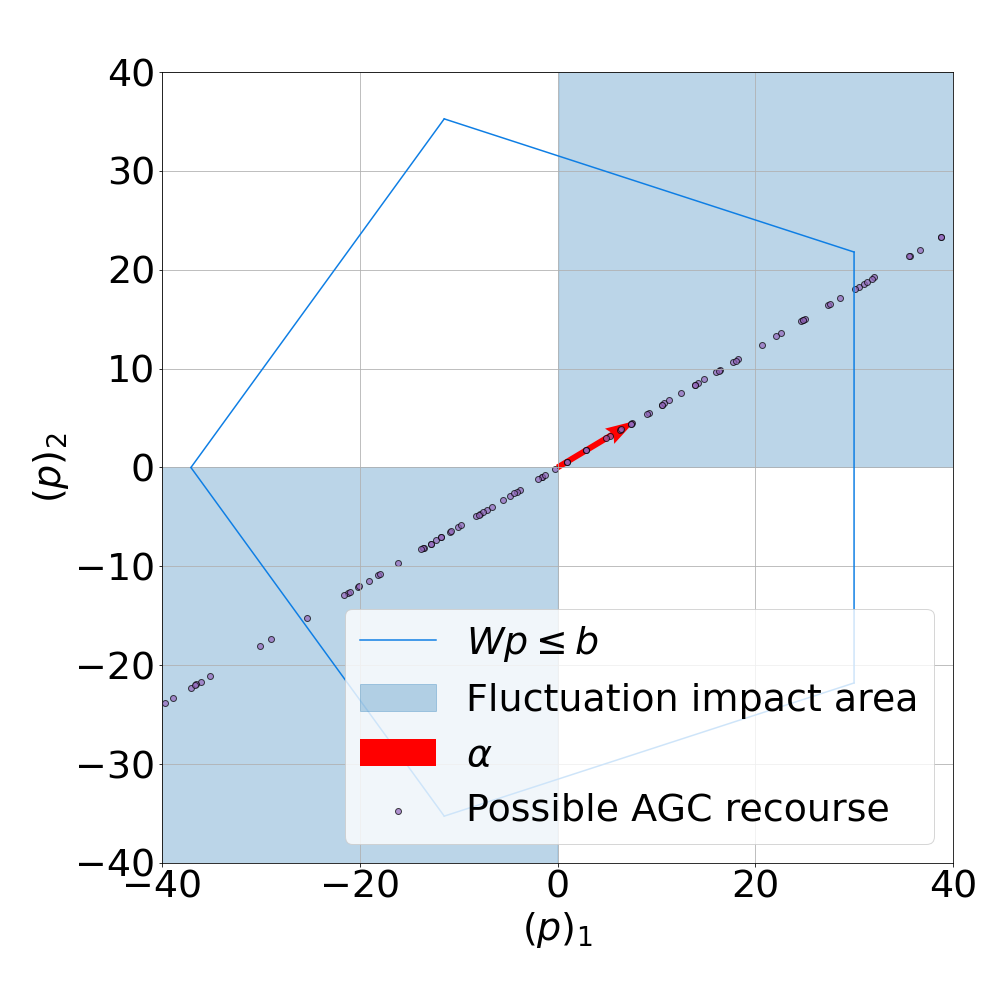
\includegraphics[width=.5\linewidth]{Dissertation/images/dynamic/poly_and_alpha.png}
%     \vspace{-5mm}
%     \caption{The interior of the blue polygon represents the feasibility set, while the brown area represents the possible generation set-points arising from  fluctuations and AGC recourse.
%     } \label{fig:alpha_and_poly}
%     \vspace{-5mm}
% \end{figure}

% \begin{figure}[hbt]
% \vspace{-3mm}
% \begin{subfigure}{.24\textwidth}
%   \centering
%   % include second image
%   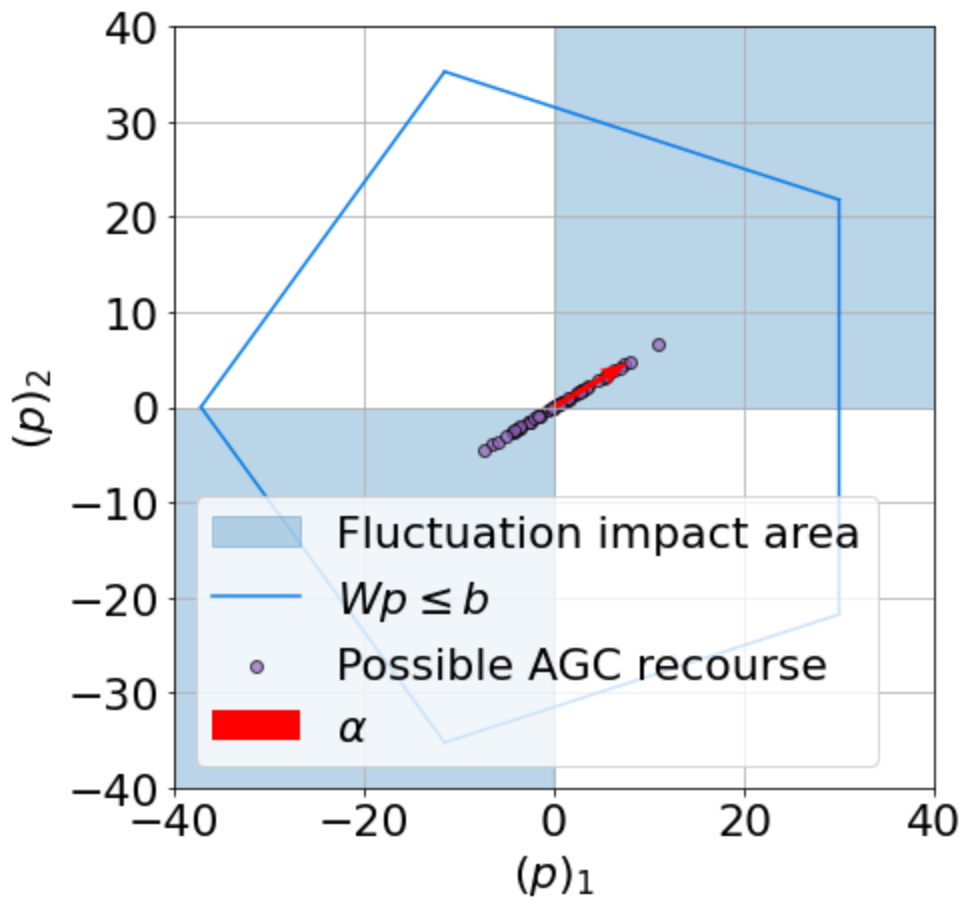
\includegraphics[width=\linewidth]{Dissertation/images/dynamic/recourse_sigma1.png}
%   \caption{Snapshot $t=1$}
%   \label{fig:t=1}
% \end{subfigure}
% % \begin{subfigure}{.24\textwidth}
% %   \centering
% %   % include second image
% %   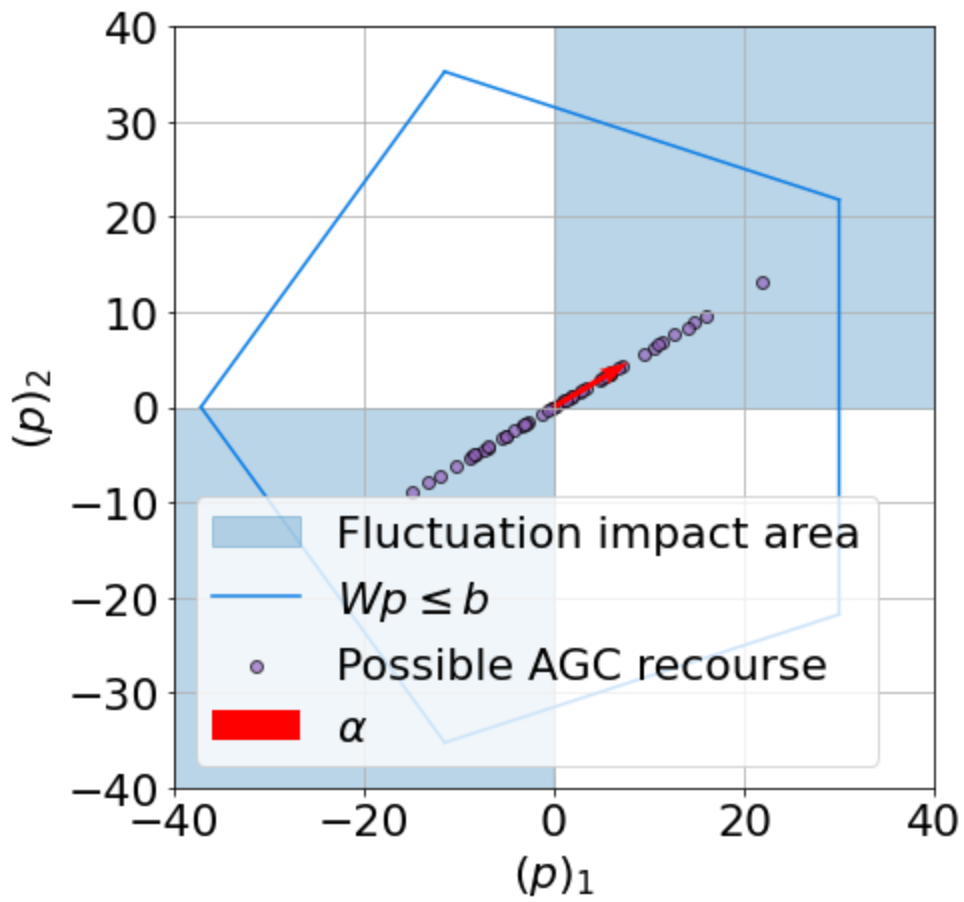
\includegraphics[width=\linewidth]{Dissertation/images/dynamic/recourse_sigma2.png}
% %   \caption{Snapshot $t=2$}
% %   \label{fig:t=2}
% % \end{subfigure}
% % \begin{subfigure}{.24\textwidth}
% %   \centering
% %   % include second image
% %   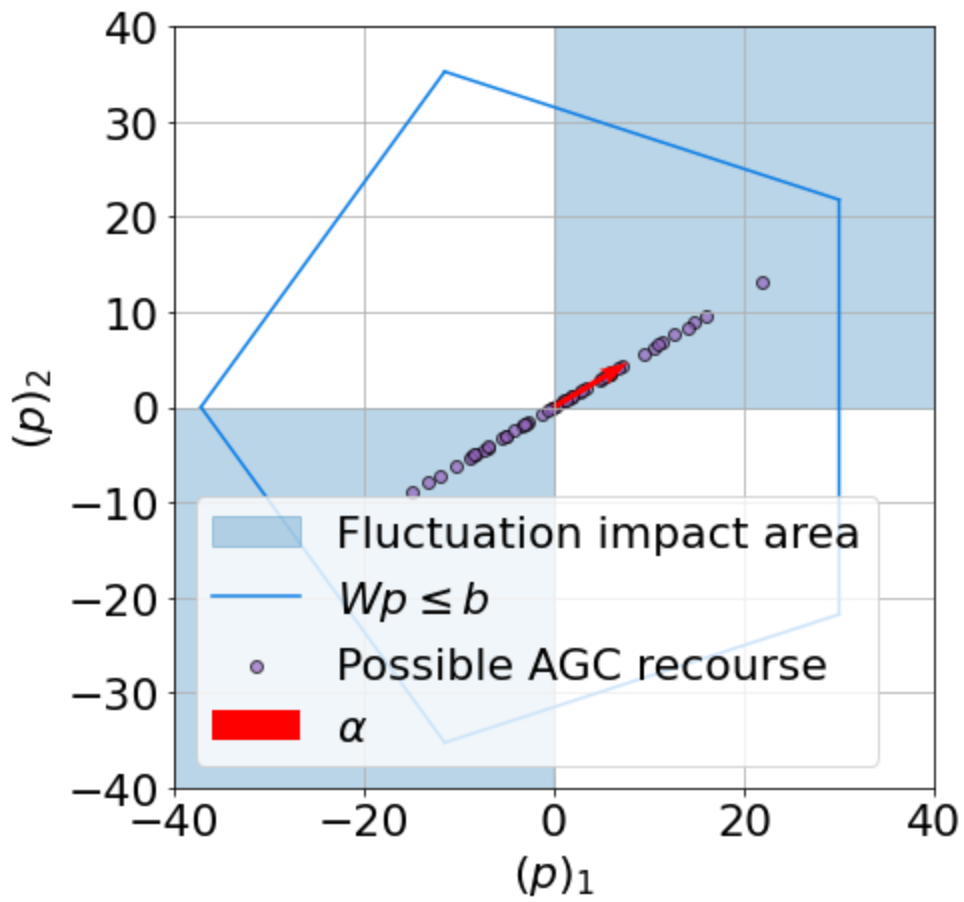
\includegraphics[width=\linewidth]{Dissertation/images/dynamic/recourse_sigma3.png}
% %   \caption{Snapshot $t=3$}
% %   \label{fig:t=3}
% % \end{subfigure}
% \begin{subfigure}{.24\textwidth}
%   \centering
%   % include first image
%   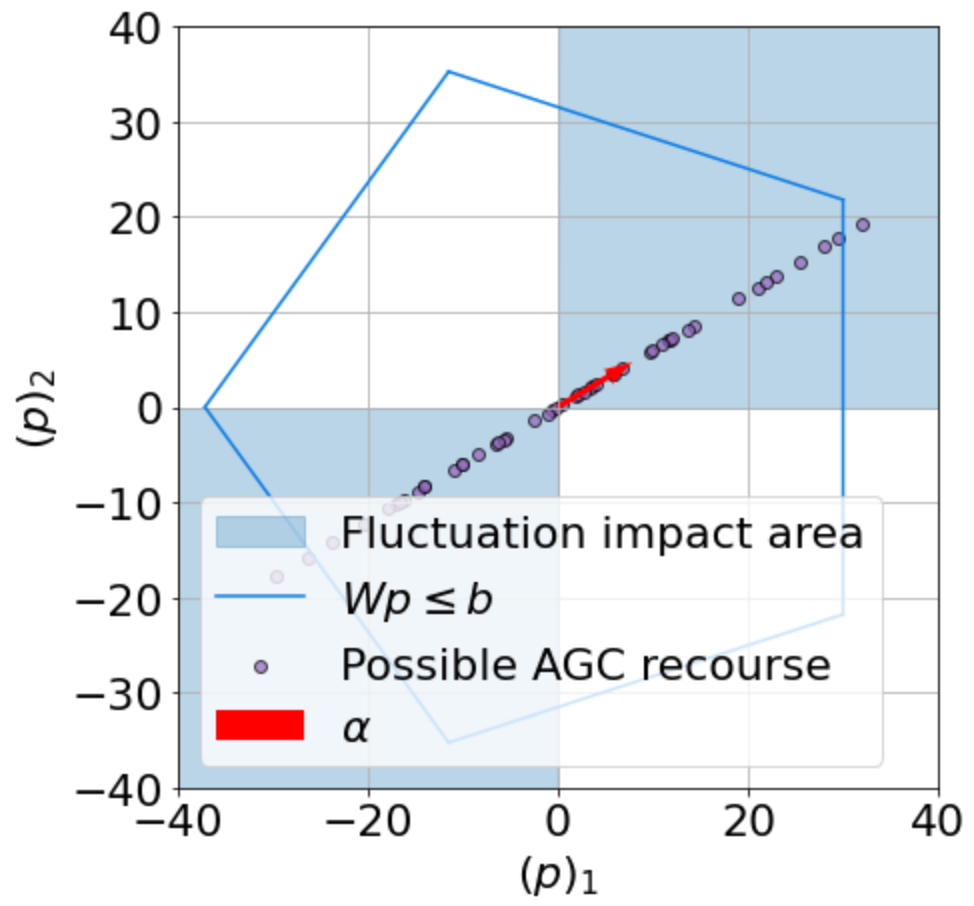
\includegraphics[width=\linewidth]{Dissertation/images/dynamic/recourse_sigma4.png}~~~~~~\hfill
%   \caption{Snapshot $t=4$}
%   \label{fig:t=4}
% \end{subfigure}
% \vspace{-5mm}
% \caption{The growth of variance of total generation demand imbalance $\sum_{\tau \le t}\xi^\tau$ with time $t$.}
% \label{fig:alpha_and_poly_snapshots}
% \end{figure}

Our next step is to derive an upper bound for the failure probability of a control strategy ${(\xi^1, \dots, \xi^T), \alpha}$ with a given starting point $p^0$. 
% To achieve this, we  utilize the following bounds on the probability of $\mathbb{P}(S_1 \cup \dots \cup S_k)$ for some arbitrary sets $S_1, \dots, S_k:$
% \begin{gather*}
%     \max_{i\le k} \mathbb{P}(S_i) \le \mathbb{P}(S_1 \cup \dots \cup S_k) \le \sum_{i\le k} \mathbb{P}(S_i)
% \end{gather*}

%In the context of this chapter, $S_i$ represents the feasibility of the system at $t=i$.
% Notice that as the power system is balanced, we have the following: 
% \begin{gather*}
%     \forall t\le T\quad \sum_{1\le k\le n} p^t_k = 0 \Rightarrow \delta p^t = \sum_{k\le n}\xi^t_k
% \end{gather*}
% thus 
% \begin{gather*}
%     p^t = p^{t-1} + \xi^t - \alpha \sum_{k\le n}\xi^t_k = p^0 + (e-\alpha) \sum_{t\le T}\sum_{k\le n} \xi_k^t, 
% \end{gather*}
% where $e$ is a unit vector, $e = (1, \dots, 1)$. 
% {\color{blue} Sasha, does it match to your equation?}

% The probability that all system states are feasible is given by $\pi = \mathbb{P}\left(\forall k, t:  \omega_k^\top p^t \leq \beta_k, \; k\le n, t\le T\right)$ and must be such as $\pi \geq 1-\eta$.
% Note that $\pi \le 1 -  \max_{k\le n,t\le T}\mathbb{P}(\omega_k^\top p^t > \beta_k)$. Also,  
% $\mathbb{P}\left(\forall i, t: \bigcup_i \omega_i^\top p^t > \beta_i\right) \le 1 -  \max_{i, t}\mathbb{P}(\omega_i^\top p^t > \beta_i)
%     %1 - \mathbb{P}(\omega^\top\sum_{t\le T}\sum_{k\le n} \xi_k^t (1-\alpha_k) < \beta - \omega^\top p^0)\\
%     $
% with $p^t\sim {\cal N}(p^0, \texttt{diag}((\sigma^1)^2, \dots, \sum_{t=1}^{T-1}(\sigma^\tau)^2))$. Now, we have the upper bound $\pi$ greater or equal than $1 - \eta$ we get 
% \begin{equation}
% \max_{i, t}\mathbb{P}(\omega_i^\top p^t > \beta_i) \leq  \eta.
% \label{eq:necessary_JCC}
% \end{equation}
% We use the latter necessary feasibility condition to get the outer approximation of the Joint Chance Constraint (JCC) in Eq.~\eqref{eq:optimal_control_2}.

% We will now derive the \emph{outer} approximation of the JCC (Joint Chance Constraint) feasibility set based on the necessary feasibility condition.
% %It is important to note that if there exists a timestamp $t$ in the range of $1$ to $T$ and a plane $\omega_i$ in the range of $1$ to $J$, such that the necessary feasibility condition \eqref{eq:necessary_JCC} does not hold, it implies that the entire JCC, Prob.~\eqref{eq:optimal_control_2}, cannot be satisfied.
% Assume that for some $t, i$ \eqref{eq:necessary_JCC} is violated.

To get an analytical sufficient condition on the redundant scenarios, we derive a necessary condition for JCC feasibility converted to a sufficient condition of not being in the JCC feasibility set. Note that there is following bound on feasibility probability from \eqref{eq:optimal_control_2}:
\begin{lemma}
    \label{lemma:bound_prob}
     Let $\pi(p^0, \alpha) \geq 1 -\eta$, where $$\pi(p^0, \alpha) = \mathbb{P}\left\{ \cap_{i, \tau} (\omega^p_i)^\top p^0 + (E^\tau_i)^\top \xi \cdot(\omega^\alpha_i)^\top \alpha \leq \beta_i\right\}.$$ Then 
    \vspace{-2mm}
    \[\max_{i, t} \mathbb{P} \left\{ (\omega^p_i)^\top p^0 + (E^\tau_i)^\top \xi \cdot (\omega^\alpha_i)^\top \alpha > \beta_i \right\} \leq 1-\pi(p^0, \alpha).\]
\end{lemma}
\begin{proof}
    As $\mathbb{P}\left\{ \cup_{i, t} (\omega^p_i)^\top p^0 + (E^\tau_i)^\top \xi \cdot (\omega^\alpha_i)^\top \alpha > \beta_i \right\} = 1 - \pi(p^0, \alpha)$, applying the Boole-Fréchet bound \cite[Theorem 4.2.1]{williamson1989probabilistic} to the left-hand side of this we prove the lemma.
\end{proof}
Lemma \ref{lemma:bound_prob} provides a handful necessary condition:
\begin{corollary}
    \label{lemma:corollary}
    Let $(p^0, \alpha)$ be feasible to JCC in \eqref{eq:optimal_control_2}. Then $$\max_{i, t} \mathbb{P} \left\{ (\omega^p_i)^\top p^0 + (E^\tau_i)^\top \xi \cdot (\omega^\alpha_i)^\top \alpha > \beta_i \right\} \leq \eta.$$
\end{corollary}
\begin{proof}
    Feasibility yields $\pi(p^0, \alpha) \geq 1 -\eta$ iff $1 - \pi(p^0, \alpha) \leq \eta$. Applying Lemma \ref{lemma:bound_prob} proves the corollary.
\end{proof}


We now formalize $\hat{\mathcal{P}}_r$ for Problem~\eqref{eq:optimal_control_2}. This gives us a-priori sufficient condition on sample redundancy.

\begin{theorem}
Let scenarios $\xi(j) \sim \mathcal{N}(0, \Sigma), ~ j \in \mathcal{I}=\{1, \dots, N\}$ form SA \eqref{eq:optimal_control_sampling_02} and a solution of this problem $(\hat{p}^0_{\mathcal{I}}, \hat{\alpha}_{\mathcal{I}})$ be feasible for the JCC problem \eqref{eq:optimal_control_2}. Moreover, assume that the cost function $c(\cdot)$ is linear.  Let $\hat{\mathcal{P}}_r = \{ \xi\in \mathbb{R}^T:~ |(E^{\tau}_i)^\top \xi|  \leq \Phi^{-1}(1 - \eta) \sigma^\tau_i \gamma ~\forall i, \tau \}$, where $\gamma \in (0, 1)$ and $(\sigma^\tau_i)^2 = (E^\tau_i)^\top \Sigma (E^\tau_i)$.
Then, first, SA  where scenarios $\xi(j), ~ j \in \mathcal{I}_r = \{ j: \xi(j) \in \hat{\mathcal{P}}_r \}$ yields solution $(\hat{p}^0_{\mathcal{I}_r}, \hat{\alpha}_{\mathcal{I}_r})$ that is not feasible for original JCC Problem \eqref{eq:optimal_control_2}. Second, SA where scenarios $\xi(j), ~ j \in \mathcal{I} \setminus \mathcal{I}_r$ yields the solution $(\hat{p}^0_{\mathcal{I} \setminus \mathcal{I}_r}, \hat{\alpha}_{\mathcal{I} \setminus \mathcal{I}_r})$ that is feasible for the original JCC Problem \eqref{eq:optimal_control_2}.
\label{th:P_r sampling polytope}
\end{theorem}
\begin{proof}
    The feasibility set of SA is given by $(w^p_i)^\top p^0 + (E_i^\tau)^\top \xi(j) \cdot (\omega^\alpha_i)^\top \alpha \leq \beta_i, ~ \forall i, \tau, j$. Since the cost function is linear for solution of SA, $\exists i', \tau', j': ~ (w^p_{i'})^\top p_{\mathcal{I}_r}^0 + (E_{i'}^{\tau'})^\top \xi(j') \cdot (\omega^\alpha_{i'})^\top \alpha_{\mathcal{I}_r} = \beta_{i'}$. Next, one has $(E^{\tau}_i)^\top \xi (j')  \leq \Phi^{-1}(1 - \eta) \sigma^\tau_i \gamma$, because $
    \xi(j') \in \hat{\mathcal{P}}_r$, positive absolute value case. This implies that $(\omega^p_{i'})^\top p^0_{\mathcal{I}_r} \geq \beta_{i'} - \Phi^{-1}(1-\eta) \sigma^{\tau'}_{i'} \| (\omega_{i'}^\alpha)^\top \alpha_{\mathcal{I}_r} \| \gamma$. However, the necessary condition from Corollary \ref{lemma:corollary} implies that $\forall i, \tau ~ (\omega_i^p)^\top p^0_{\mathcal{I}_r} \leq \beta_i - \Phi^{-1}(1-\eta) \sigma^\tau_i \| (\omega_i^\alpha)^\top\alpha_{\mathcal{I}_r}\|$. Recalling that $\gamma \in (0, 1)$ we obtain contradiction that leads to the fact that $(\hat{p}_{\mathcal{I}_r}^0, \hat{\alpha}_{\mathcal{I}_r})$ is infeasible for original JCC Problem.
    Now drop redundant scenarios from the SA. Since $(\hat{p}^0_{\mathcal{I}}, \hat{\alpha}_{\mathcal{I}})$ is feasible for JCC problem and data samples $\xi(j), ~ j \in \mathcal{I}_r$ do not contribute to the feasibility, then SA solution $(\hat{p}_{\mathcal{I} \setminus \mathcal{I}_r}^0, \hat{\alpha}_{\mathcal{I} \setminus \mathcal{I}_r})$ built on $\xi(j), ~ j \in \mathcal{I} \setminus \mathcal{I}_r$ is feasible for JCC problem.
\end{proof}

\begin{comment}
{\color{orange}
\begin{theorem}[NVC - Necessary Violation Criterion]
    \label{th:NVC}
    Let $p^0 \in \mathbb{R}^{n_g}, \alpha \in \mathbb{R}^{n_g}$. A pair $p^0, ~ \alpha$ does not satisfy $\max_{i, t} \mathbb{P} \left\{ \omega^\top_i p^t > \beta_i \right\} \leq \eta$ $\iff$ $\exists i, t, \omega_i^\top \alpha \neq 0: ~ \omega_i^\top p^0  > \beta_i - \Phi^{-1}(1-\eta)\tilde{\sigma}^t \| \omega_i^\top \alpha \|$, where $\Phi(\cdot)$ is a CDF of standard normal Gaussian r.v. 
\end{theorem}
\begin{proof}
    A pair $p^0, ~\alpha$ does not satisfy $\max_{i, t} \mathbb{P} \left\{ \omega^\top_i p^t > \beta_i \right\} \leq \eta$ $\iff$ $\exists i, t, \omega_i^\top \alpha \neq 0: ~ \mathbb{P}\left\{ \omega^\top_i p^0 + \omega_i^\top \alpha \zeta^t > \beta_i \right\} > \eta$. The latter is equivalent to $\Phi\left( \frac{\omega_i^\top p^0}{\tilde{\sigma}^t \| \omega_i^\top \alpha \|} \right) > \eta$, which, due to the monotonicity of the CDF, can be setup as $\omega_i^\top > \beta_i - \Phi^{-1}(1 - \eta) \tilde{\sigma}^t \| \omega_i^\top \alpha \|$.
\end{proof}
Based on violation criteria \ref{th:NVC} we present formal description of scenario necessarial non-redundancy.
\begin{definition}
    \label{def:necessary_non-redundant}
    Let SA \eqref{eq:optimal_control_sampling_02} be based on scenarios $\xi^t(j), ~ j \in \mathcal{I} = \{1, \dots, N \}$. Scenarios indexed with $\mathcal{I}_{NNR},~ \mathcal{I}_{NNR} \subset \mathcal{I}$ are called Necessarily Non-Redundant (NNR) $\iff$  $\forall i,~ \forall j \in \mathcal{I}_{NNR}$ $\sign(\omega_i^\top \alpha) \zeta^t (j) > \Phi^{-1}(1 - \eta) \tilde{\sigma}^t $.
\end{definition}
\begin{definition}
    \label{def:sufficiently_redundant}
    Let SA \eqref{eq:optimal_control_sampling_02} be based on scenarios $\xi^t(j), ~ j \in \mathcal{I} = \{1, \dots, N \}$. Scenarios indexed with $\mathcal{I}_{SR},~ \mathcal{I}_{SR} \subset \mathcal{I}$ are called Sufficiently Redundant (SR) $\iff$  $\forall i,~ \forall j \in \mathcal{I}_{SR}$ $\sign(\omega_i^\top \alpha) \zeta^t (j) < \Phi^{-1}(1 - \eta) \tilde{\sigma}^t \gamma $, where $\gamma = \min_{i, ~\alpha: \|\alpha - \alpha_0\|_2 \leq \delta \alpha, ~ \omega_i^\top \alpha \neq 0} \| \omega_i^\top \alpha \|.$
\end{definition}
Evidently, a scenario cannot be simultaneously NNR and SR.
The next theorem reveals the purpose of the definitions above and allows one to classify scenarios based on redundancy.
\begin{theorem}
    \label{th:redundancy_classify}
    Let SA \eqref{eq:optimal_control_sampling_02} be based on scenarios $\xi^t(j), ~ j \in \mathcal{I} = \{1, \dots, N \}$. Also, let $c(p^t)$ be linear and the solution of SA with scenarios $\mathcal{I}$ $(\hat{p}^0, \hat{\alpha})$ be feasible for JCC. Then, SR scenarios with indexes $\mathcal{I}_{SR}$ are redundant.
\end{theorem}
\begin{proof}
    Let us consider SA built only on SR scenarios. This yields that the solution of such scenario approx $(\hat{p}^0_{\mathcal{I}_{SR}}, \hat{\alpha}_{\mathcal{I}_{SR}}).$ Due to the  From the definition of SR scenarios, we have that $\omega^\top_i \hat{p^0} \leq \beta_i - \Phi^{-1}(1-\eta) \tilde{\sigma}^t \gamma ~ \forall ~i, t$. Moreover, due to the linearity of the cost function, $\exists k, j: \omega_k^\top \hat{p}^0 = \beta_k - \omega_k^\top \alpha \zeta^t(j)$. Since $\zeta^t(j)$ is a SR scenario and $\sign(x) = x / \|x\|, ~ x \neq 0$, one obtains,  $\omega_k^\top \hat{p}^0 \geq \beta_i - \Phi^{-1}(1-\eta)\tilde{\sigma}^t \gamma$ for this constraint. Moreover, since $\gamma \leq \| \omega_k^\top \alpha \|$, one obtains $\omega_k^\top \hat{p}^0 \geq \beta_i - \Phi^{-1}(1-\eta)\tilde{\sigma}^t \| \omega_k \alpha \|$. Using Th. \ref{th:NVC} and Corollary \ref{lemma:corollary} one obtains that those scenarios lead to infeasible, for JCC, solution. So, each NR scenario is redundant by definition.
\end{proof}
}
\end{comment}
\begin{comment}
{\color{orange}
Moreover, right-hand sides of the inequalities decrease from deterministic $\beta_i$ as $\tilde{\sigma}^t = \sqrt{\sum_{\tau=1}^{t-1} (\sigma^\tau)^2}$ grows. Figure~\ref{fig:evoluted} illustrates the mutual geometry between initial feasibility polytope and necessary feasibility polytope at $t > 1$. It's worth noting that since $\Delta_i^t$ depends on $| \omega_i^\top \alpha |$, the planes that are closer to being orthogonal to the participation vector $\alpha$ are less impacted by the uncertainty in control policy.
}
\end{comment}
%In other words, such planes of $\mathcal{P}_{out}$ have slower decreasing right hand side.
% \begin{remark}
% Additionally, the same reasoning applies to the ramp-up and ramp-down constraints $|\alpha_k \xi^t| \leq R_k$. In this case, the logic remains unchanged for the hyperplanes $\alpha_i\xi^t \leq R_i$. It's important to note that $|\alpha_k \xi^t| \leq R_k$ is equivalent to the simultaneous satisfaction of $\alpha_k \xi^t \leq R_k$ and $-\alpha_k \xi^t \leq R_k$.
% \end{remark}
\begin{comment}
\begin{figure}
    \begin{subfigure}{.24\textwidth}
        \centering
        % \vspace{-3mm}
        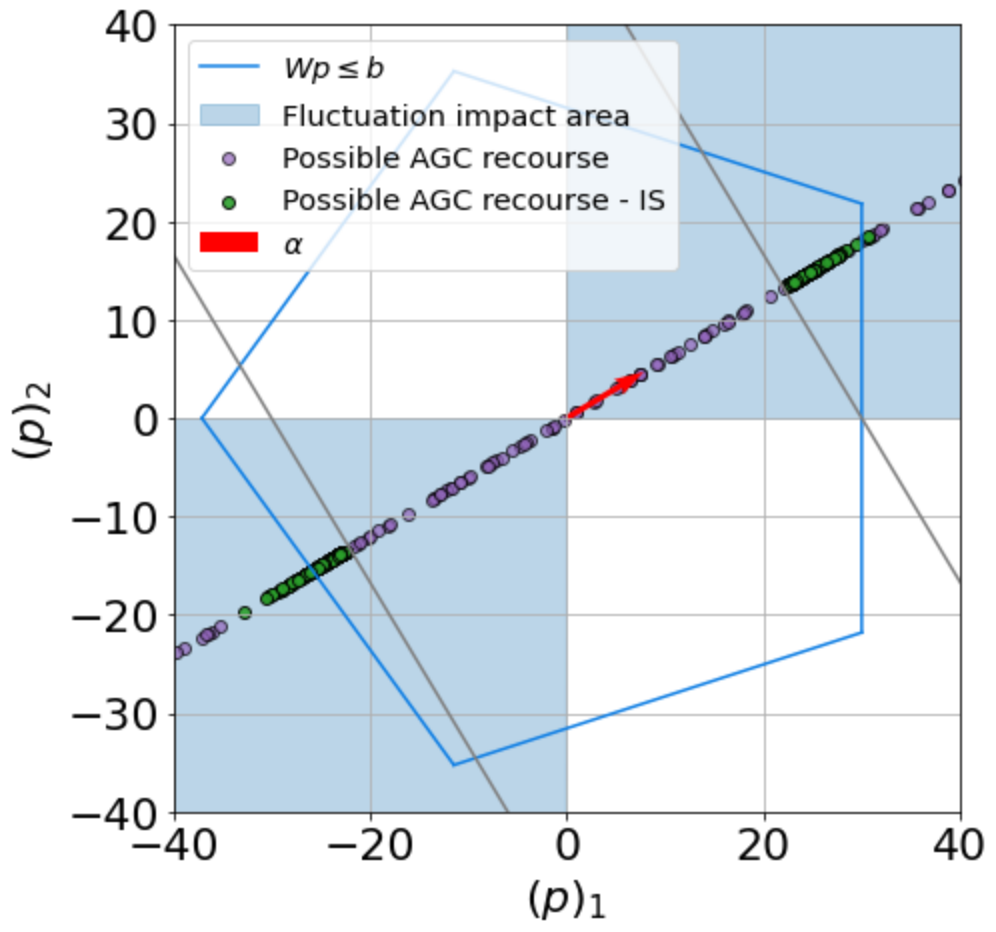
\includegraphics[width=.8\textwidth]{Dissertation/images/dynamic/poly_and_alpha_mc_vs_is.png}
        \vspace{-2mm}
        \caption{AGC recourses from non-redundant sample set $\mathcal{P}_r$ that lead to violation of technical limits.
        }
        \label{fig:importance_sampled_vs_mc}
        \vspace{-5mm}
    \end{subfigure}
    \begin{subfigure}{.24\textwidth}
        \centering
        \vspace{-3mm}
        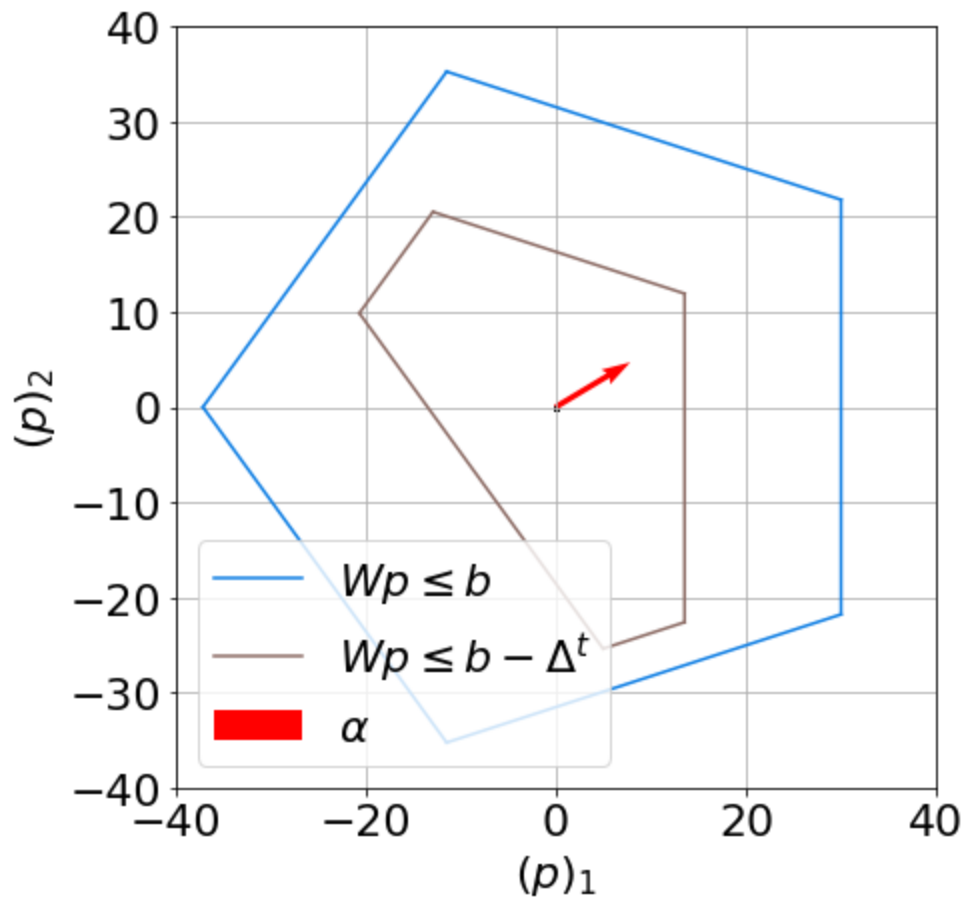
\includegraphics[width=.8\textwidth]{Dissertation/images/dynamic/necessary_poly.png}
        \vspace{-2mm}
        \caption{Mutual position of the deterministic feasibility polygon $Wp_g \leq b$ and $\mathcal{P}_{out}$. }
        \label{fig:evoluted}
        \vspace{-5mm}
    \end{subfigure}
    \label{fig:demo}
    \caption{\color{orange} The impact of uncertainty on feasibility sets and AGC.}
    \vspace{-4mm}
\end{figure}
\end{comment}
Theorem \ref{th:P_r sampling polytope} establishes a sufficient, i.e., a priori condition on sample redundancy across a given dataset $\xi(j), j \in \mathcal{I}$ that guarantees a feasible solution. Specifically, if a dataset provides assurance of producing a feasible solution for the original JCC problem, samples within $\hat{\mathcal{P}}_r$ may be disregarded. Thus this theorem offers a way to assess the dataset's potential a-priori: if all data samples fall within $\mathcal{P}_r$, it is be impossible to derive any feasible solution for the JCC from this data.
%$\zeta(j) = (\zeta^1(j),\dots, \zeta^T(j)) \sim \mathcal{N}(0, \Sigma_{\zeta})$ outside of the polytope $\underline{P}_{r} = \left\{ (\zeta^1, \dots, \zeta^T)^\top: ~ \omega_i^\top \alpha \zeta \leq \Phi^{-1}(1 - \eta) \| \omega_i^\top \| \tilde{\sigma}^t \gamma , ~ \forall~ t,~ \forall~ i\right\}$ to increase data efficiency of the SA. 
%{\color{red} Should I delete this?}
%{ \color{gray}
%The polytope can equally be described as $\mathcal{P}_{r} = \left\{ \mathbf{\zeta}: ~ \mathcal{W} \mathbf{\zeta} \leq \Phi^{-1}(1-\eta) \mathcal{S}\right\}$. 
%Here $\mathcal{W} \in \mathbb{R}^{(J \cdot T) + (2 \cdot n_g \cdot T)\times T}$ is a block diagonal matrix. The $j^{\textup{th}}$ block of the matrix is of a shape $T \times T$ and $\mathcal{W}_j =  \sign(\omega_k^\top \alpha) \cdot I$ where $j \in 1 + (k - 1) \cdot T, \dots, k \cdot T $, $k=1, \dots, J$. The other blocks correspond to the ramp-up/down constraints. They are as follows: $\mathcal{W}_j=I$ for $j\in J\cdot T + 1 + (k-1) \cdot T, \dots J\cdot T + 1 + k \cdot T$ and $k=1, \dots, n_g$. The remaining blocks of the matrix are the same except the sign and correspond to the ramp-down constraints. The vector on right-hand side is $\mathcal{S} = (\mathcal{S}_{\mathcal{W}}, \mathcal{S}_{ramp})$, where $\mathcal{S}_{\mathcal{W}}= (\tilde{\sigma}^1, \dots, \tilde{\sigma}^T, \dots,  \tilde{\sigma}^1, \dots, \tilde{\sigma}^T)$ and 
%\[\mathcal{S}_{ramp} =\left[\frac{R_1}{\alpha_1 \sigma^1}, \dots, \frac{R_{n_g}}{\alpha_{n_g} \sigma^1}, \dots,
%\frac{R_1}{\alpha_1 \sigma^T}, \dots, \frac{R_{n_g}}{\alpha_{n_g} \sigma^T}\right].\] 
%Overall, $ \mathcal{S} \in \mathbb{R}^{J \cdot T + 2 \cdot n_g \cdot T}$.
%}
%{\color{red} Should I delete this?}

%\vspace{-4mm}
\subsection{SA Solution Guarantees and Dataset Complexity}
In this section we provide theoretical guarantees on the solution of reduced SA that does not contain redundant samples within $\hat{\mathcal{P}}_r$.
The following theorem addresses the sampling complexity of the SA with data samples indexed $\mathcal{I} \setminus \mathcal{I}_r$.
\begin{theorem}\label{thm:40}
Let $(\hat{p}^0, \hat{\alpha})$ be a unique solution of the SA Problem~\eqref{eq:optimal_control_sampling_02} with $N$ i.i.d. samples, so that none of the samples belong to $\hat{\mathcal{P}}_{r}$. Moreover, assume that for any $N$ the assumption \ref{asmp:10} is fulfilled. Then for any $\rho \in (0,1)$ and any~$\eta \in (0, 1/2]$, $(\hat{p}^0, \hat{\alpha})$ is also a solution for the Chance-constrained optimal power flow Problem~\eqref{eq:optimal_control_2} with probability at least $1-\rho$ if 
$%\begin{align*}
  N \ge \left\lceil 2\eta^{-1}(1-\nu)\ln \frac{1}{\rho} + 2d + 2d\eta^{-1}(1-\nu) \ln\frac{2(1-\nu)}{\eta} \right\rceil, 
$%\end{align*} 
 where $d$ is a dimension of the space of controllable generators and participation factors, i.e., $d = 2 n_g$, and $\nu$ is the probability of a random scenario $\xi \sim \mathcal{N}(0, \Sigma)$ to belong to $\hat{\mathcal{P}}_{r}$, and $\nu < 1$. 
\end{theorem}
\begin{proof}
First, notice that discarding random scenarios $\xi \notin \hat{\mathcal{P}}_{r}$ is equivalent in solving the SA problem with sampling 
$\xi$ from a distribution $\mathcal{D}$ where  
$\xi \sim \mathcal{D} \Leftrightarrow \xi\sim \mathcal{N}(0, \Sigma) \textup{s. t. } \xi\not\in \hat{\mathcal{P}}_{r}$. 
From the theorem statement, $1-\nu$ is the probability mass associated with samples in $\xi\sim \mathcal{N}(0, \Sigma)$ 
that are outside $\hat{\mathcal{P}}_{r}$.
%
 Assumption \ref{asmp:10} and convexity of each function in Problem \ref{eq:optimal_control_2} meet the conditions of Calafiori and Campi~\cite[Theorem 1]{calafiore2006scenario} implying that for any probability $\rho \in (0,1)$ and any confidence threshold probability $\varepsilon$, and dimension of the space of parameters $d$ one has, for~$N_1$
\vspace{-1mm}
\begin{align}\label{eq:mon}
\vspace{-2mm}
  N_1 \ge \left\lceil 2\varepsilon^{-1} \ln (1/\rho) + 2d + 2d\varepsilon^{-1} \ln (2/\varepsilon)\right\rceil 
\end{align}
%\vspace{-1mm}
scenarios from $D$ and the optimal solution 
$(\hat{p}^0, \hat{\alpha})$ of the Problem~\eqref{eq:optimal_control_sampling_02}, 
%(\textcolor{red}{or (9)?})
the probability of failure is bounded as $
  \mathbb{P}_D\{(\hat{p}^0, \hat{\alpha}) \textup{ is feasible for \ref{eq:optimal_control_2}}\} \geq 1-\varepsilon
$ with prob. at least $1-\rho$. 

Notice, that the bounds on the number of samples (see Eq.~\eqref{eq:mon}) is strictly decreasing in $\varepsilon$ for $\varepsilon \in (0,1)$. As scenarios in $\hat{\mathcal{P}}_{r}$ are redundant and do not contribute to overall solution reliability, to get a probability of failure $\eta$ according to measure $\mathcal{N}(0, \Sigma)$, we need the failure probability according to $\mathcal{D}$ to be at least $\varepsilon = \eta/(1-\nu)$.  
Thus, using $\varepsilon = \eta/(1-\nu)$ and monotonicity of~Ineq.~\eqref{eq:mon} one completes the proof. 
\end{proof}


% Although, in practice, it is impossible to draw samples from $\mathcal{D}$. Thus, the next subsection is devoted to practical sampling form mixture and theoretical implications of it.


%$$
%\begin{aligned}
%\mathbb{P}\Big( (p_0, \alpha) \in \mathcal{P} \Big)&=\mathbb{P}\Big( \mathcal{W}^p p_0 + \mathcal{W}^{\alpha} \alpha \circ \Pi \vec{\xi} \leq \beta \Big) =\\
%&\mathbb{P}\Big( \cap_{i=1}^{J}\mathcal{W}^p_i p_0 + \mathcal{W}^{\alpha}_i \alpha \circ \Pi_i \vec{\xi} \leq \beta_i \Big) =\\
%&1 - \mathbb{P}\Big( \cup_{i=1}^{J}\mathcal{W}^p_i p_0 + \mathcal{W}^{\alpha}_i \alpha \circ \Pi_i \vec{\xi} > \beta_i \Big) \leq\\
%&1 - \max_{i=1, \dots,J}\mathbb{P}\Big( \mathcal{W}^p_i p_0 + \mathcal{W}^{\alpha}_i \alpha \circ \Pi_i \vec{\xi} > \beta_i \Big)
%\end{aligned}
%$$
% One can see that if there is a plane $i$ that for some initial generation set-point $p_0$ and participation factors $\alpha$ such that $\mathbb{P}\Big( \mathcal{W}^p_i p_0 + \mathcal{W}^{\alpha}_i \alpha \circ \Pi_i \vec{\xi} > \beta_i \Big) > \eta$ then the whole JCC has probability less than $1-\eta$ to satisfy, making this a necessary condition for JCC feasibility. On the other hand, the fact that $\max_{i=1, \dots,J}\mathbb{P}\Big( \mathcal{W}^p_i p_0 + \mathcal{W}^{\alpha}_i \alpha \circ \Pi_i \vec{\xi} > \beta_i \Big) \leq \eta$ does not mean that JCC is satisfied, thus, it is not sufficient feasibility condition. 
% Nevertheless, we will use this necessary condition to construct \emph{outer} approximation of $\mathcal{F}$, which will turn out to be inner approximation of deterministic polytope under probability. Using that, we will define which scenarios can be dropped from the scenario approximation without any consequence, i.e., \emph{redundant} scenarios.
% Thus, to satisfy the necessary condition, current operating point should satisfy. Denoting $\Sigma^{1/2} = \texttt{diag}(\sigma_1, \dots, \sigma_T)$
% $$
% \begin{aligned}
% \eta &\geq \mathbb{P}\Big( \mathcal{W}^p_i p_0 + \mathcal{W}^{\alpha}_i \alpha \circ \Pi_i \vec{\xi} > \beta_i \Big) =\\
% &\mathbb{P}\Big( \frac{\mathcal{W}^{\alpha}_i \alpha \circ \Pi_i \vec{\xi}}{\| \Sigma^{1/2} \mathcal{W}^{\alpha}_i \alpha \circ \Pi_i \|} >\frac{\beta_i - \mathcal{W}^p_i p_0}{\| \Sigma^{1/2} \mathcal{W}^{\alpha}_i \alpha \circ \Pi_i \|} \Big) =\\
% &\Phi\left( \frac{\beta_i - \mathcal{W}^p_i p_0}{\| \Sigma^{1/2} \mathcal{W}^{\alpha}_i \alpha \circ \Pi_i \|} \Big) \right)
% \end{aligned}
% $$
% Here $\Phi$ is the cdf of standard normal distribution. The condition can be reformulated in terms of the following set:
% $\mathcal{P}_{in} = \{ (p_0, \alpha): \mathcal{W}^p_i p_0 \leq \beta_i - \Phi^{-1}(1-\eta) \| \Sigma^{1/2} \mathcal{W}^\alpha_i \alpha \circ \Pi_i\|\}$. One can observe that for fixed $\alpha = \alpha_0$ this set is the polytope in $p_0$ (initial generation set-point) that defines inner approximation for feasibility set.
% %To define a condition on sample redundancy one must consider inner approximation of non-convex chance-constrain feasibility set. This is easily achieved if one considers Single Chance Constraint (SCC) formulation instead of more accurate Joint Chance Constraint (JCC) as in Problem \ref{eq:optimal_control_1}.
% %The SCC is built from the constraints of the following form: $\mathbb{P} (\omega_i^\top p_0 > b_i - \omega_i^\top \alpha_0 \xi_t) \leq 1 - \eta$. One may rewrite is at $\mathbb{P}\left( \textup{sign}(\omega_i^\top \alpha_0) \xi_t / \sigma_t > \frac{b_i - \omega_i^\top p_0}{|\omega_i^\top \alpha_0|} \right) < \eta$, which is equivalent to $w_i^\top p_0 \leq b_i - \Phi^{-1}(1 - \eta) \sigma_t |\omega_i^\top \alpha_0| $. If one brings the stochastic part back into this constraint, one would obtain $w_i^\top p_0 + \omega_i^\top \alpha_0 \xi_t \leq b_i + \Phi^{-1}(1 - \eta) \sigma_t |\omega_i^\top \alpha_0| $. From here it is evident that if $\xi_t$ is such that $\omega_i^\top \alpha_0 \xi_t \leq \Phi^{-1}(1 - \eta) \sigma_t |\omega_i^\top \alpha_0|$ then $p_0$ satisfies this constraint. Next, one can construct a polytope for realization $\xi_\tau, ~ \tau=1, \dots, T$ -- the trajectories of disturbances that would lead to no violation of constraints. Next, considering only those samples that are out of it, a more efficient scenario approximation is constructed. Let us denote this polytope as $\mathcal{P}_0 = \Big\{ (\xi^1, \dots, \xi^T):~ \omega_i^\top \alpha_0 \xi_t \leq \Phi^{-1}(1 - \eta) \sigma_t |\omega_i^\top \alpha_0|,$ $t=1, \dots, T, ~ i=1, \dots, m  \Big\}$.
% {\color{red} Now we discuss the process of sampling non-redundant scenarios. Let us consider AGC recourse differences for $T$ snapshots and its effect due to a realization of perturbation $\vec{\xi}^i$ and compare it to the necessity fix given by }
% \begin{equation}
%     \mathcal{W}_i \alpha \circ \Pi_i \vec{\xi}^i - \Phi^{-1}(1 - \eta) \| \Sigma^{1/2} \mathcal{W}^\alpha_i \alpha_0 \circ \Pi_i \|.
%     \label{eq:sample_redundancy}
% \end{equation} {\color{red} If this difference is non-negative then one would obtain that the scenario $\vec{\xi}^i$ does not drive generation set-point sequence out of the feasibility region contributing none to the infeasibility modeling which is essential for construction of scenario spproximation. Otherwise, it does. Thus, the condition of sample redundancy is given by eq. \ref{eq:sample_redundancy}. The scenario approximation should be constructed with samples drawn outside of this polytope $\mathcal{P}_0$.}
% % Now we discuss the process of sampling of productive scenarios. The goal is to obtain samples $(\xi^1, \dots, \xi^T)_i$ that lie out of $\mathcal{P}_0$. Let us consider $T$ snapshots and assume that $\xi_\tau \sim \mathcal{N}(0, \sigma^2_\tau)$. Note that both the initial generation set-point and AGC recourse must satisfy feasibility constraints. One can write these constraints in a compact notation: $\mathbb{P}\left(W_T p_0 + W_T\alpha \circ \Pi_T \vec{\xi} \leq b_T\right) \geq 1-\eta$. 
% % Thus, $\mathcal{P}_0$ can be equivalently defined as $\mathcal{P}_0 = \Big\{ \vec{\xi}:~ (W_T \alpha_0 \circ \Pi_T) \vec{\xi} \leq \Phi^{-1}(1 - \eta) |W_T \alpha_0| \circ \Pi_T \cdot (\sigma_1, \dots \sigma_T)^\top  \Big\}$. 
% % Sampling realizations of random vectors out of $\mathbb{P}_0$ can be conducted using ALOE {\color{red} cite MC} algorithm. ALOE allows one to obtain samples that are conditioned to be located of the polytope specified. In our case, we choose $\mathcal{P}_0$ to sample out of. In other words, we sample realizations of $\vec{\xi} \sim D_{\mathcal{P}_0}$, where $D_{\mathcal{P}_0} \sim \mathcal{N}(0, \texttt{diag}(\sigma_1^2, \dots, \sigma_T^2), ~ \vec{\xi} \notin \mathcal{P}_0$.
%\vspace{-3mm}
% START OF SAMPLING
\begin{comment}
\subsection{Sampling non-redundant scenarios}
\label{sec:sampling}

In order to sample non-redundant scenarios, we approximate their distribution with a distribution mixture $D$ that has the density $f_D(x) = \sum_{i=1}^{|\mathcal{S}|}w_i f_{D_i} (x).$ Here $|\mathcal{S}| = J \cdot T + 2 \cdot n_g \cdot T$, mixture components' weights are positive and $\sum_{i} w_i  = 1$, $f_{D_i}$ are mixture components densities. The mixture components are Gaussians conditioned on a single linear constraint's complement. For a plane $i$: $\xi \sim D_i \Longleftrightarrow \mathcal{N}(0, \Sigma), ~ \mathcal{W}_i^\top x > \mathcal{S}_i$. The exact expression for the density is $f_{D_i} = \textbf{1} (\mathcal{W}_i^\top x > \mathcal{S}_i) f(x) / \mathbb{P}(\mathcal{W}_i^\top x > \mathcal{S}_i)$, where the probability also has explicit expression: $\mathbb{P}(\mathcal{W}_i^\top x > \mathcal{S}_i) = \Phi(-\mathcal{S}_i / \| \Sigma^{1/2}_{\zeta} \mathcal{W}_{i} \|)$. Such mixture has proven to be useful in approximating the distribution of interest \cite{lukashevich2021importance}, \cite{lukashevich2021power}, \cite{owen2019importance}. For this study, we use $w_1 = \dots = w_{|\mathcal{S}|}$.

In order to sample from this mixture, one must pick a plane with probability $w_i$ and then sample outside of this plane.
The Algorithm \ref{alg:sample1d} summarizes the procedure to produce samples outside of a plane of $\mathcal{P}_r = \{ \xi\in \mathbb{R}^T:~ (E^{\tau}_i)^\top \xi \cdot \sign[ (\omega^{\alpha}_i)^\top \alpha] \leq \Phi^{-1}(1 - \eta) \sigma^\tau_i \gamma ~\forall i, \tau \}$. 
\begin{algorithm}[H]
 \caption{Sampling $\xi \sim\mathcal{N}(\mu,\Sigma)$ s.t. $\xi^\top \omega_i \geq b_i$}
 \label{alg:sample1d}
 \begin{algorithmic}[1]
 \renewcommand{\algorithmicrequire}{\textbf{Input:}
 }
 \Require Mean $\mu$, covariance $\Sigma$, and a constraint $p^\top \omega^i \le b_i$.
 \renewcommand{\algorithmicensure}{\textbf{Output:}}
 \Ensure  $p\sim\mathcal{N}(\mu,\Sigma)$ s.t. $p^\top \omega^i \ge b_i$
 %\\ \textit{Initialisation}: 
  \State  Sample $z \sim \mathcal{N}(0, I_n)$ and $u \sim U(0,1)$
  \State  Compute $y = \Phi^{-1}(\Phi(\tau) + u(1 - \Phi(\tau)))$
  \State Set $\phi = \bar\phi y + (I_n - \bar\phi\phi^\top) z$, with $\bar\phi = \Sigma^{1/2} \omega^i / \|\Sigma^{1/2} \omega^i\|_2$\!\!
  \Return $p = \Sigma^{1/2} (\phi+\mu)$
 \end{algorithmic}
 \end{algorithm}

With given samples $\xi^t(j)$ where $j=1, \dots, N$ and $t=1, \dots, T$, we can now construct the scenario approximation \ref{eq:optimal_control_sampling_02}. Figure \ref{fig:importance_sampled_vs_mc} shows the difference between the samples obtained from the importance sampling procedure described above and the classical Monte Carlo (MC) approach as a sampler.

To analyze the sampling complexity using this proxy distribution, one needs to figure out the interrelation between density of proxy distribution and exact distribution that is Gaussian without $\mathcal{P}_r$. From \cite{lukashevich2021power} one has:

\begin{theorem}\label{thm:50}
Let $q_D(x)$, $f_D(x)$ be PDFs  of $\xi \sim\mathcal{N}(0, \Sigma) \st \xi\not\in\mathcal{P}_{r}$, and a mixture density resp. Then for any $\xi\not\in\mathcal{P}_{r}$, we have
\begin{align}\label{eq:M}
  q_D(\xi) \le M f_D(\xi),  
  M = \frac{\sum_{i\le J} \Phi(-\Delta_i/\|\Sigma^{1/2}\omega_i\|_2)
  }{\max_{i\le J}\Phi(-\Delta_i/\|\Sigma^{1/2}\omega_i\|_2)}.
\end{align}
\end{theorem}

Having the interrelation between densities, we can now prove the sampling complexity of SA based on proxy mixture:
\begin{theorem}\label{thm:80}
Let $(\hat{p}^0, \hat{\alpha})$ be a unique solution of the SA Problem~\eqref{eq:optimal_control_sampling_02} with $N$ i.i.d. samples follow mixture distribution$D$. Moreover, assume that for any $N$ the assumption \ref{asmp:10} is fulfilled. Then for any $\rho \in (0,1)$ and any~$\eta \in (0, 1/2]$, $(\hat{p}^0, \hat{\alpha})$ is also a solution for the chance-constrained optimal power flow Problem~\eqref{eq:optimal_control_2} with probability at least $1-\rho$ if 
\begin{align*}
  N \ge \left\lceil Z\ln \rho^{-1} + 2d + d Z\ln Z \right\rceil, 
\end{align*} 
where $Z = 2M\eta^{-1}(1-\nu)$, $d$ is a dimension of the problem and $\nu$ is a probability of a random scenario $\zeta$ to belong to $\mathcal{P}_{r}$, $\nu < 1$, and constant $M$ is defined by Theorem~\ref{thm:50}.
\end{theorem}
\begin{proof}
The proof is similar to the one of Theorem~\ref{thm:40}. Application of theorem \ref{thm:50} allows to upper-bound the probability of an event in measure $D$ with respect to its probability in measure $\mathcal{N}(0,\Sigma_{\zeta}) \st \zeta\not\in\mathcal{P}_{r}$. 
\end{proof}
\end{comment}
% END OF SAMPLING
%\vspace{-1mm}
%  \begin{figure}
%     \centering
%     \vspace{-3mm}
%     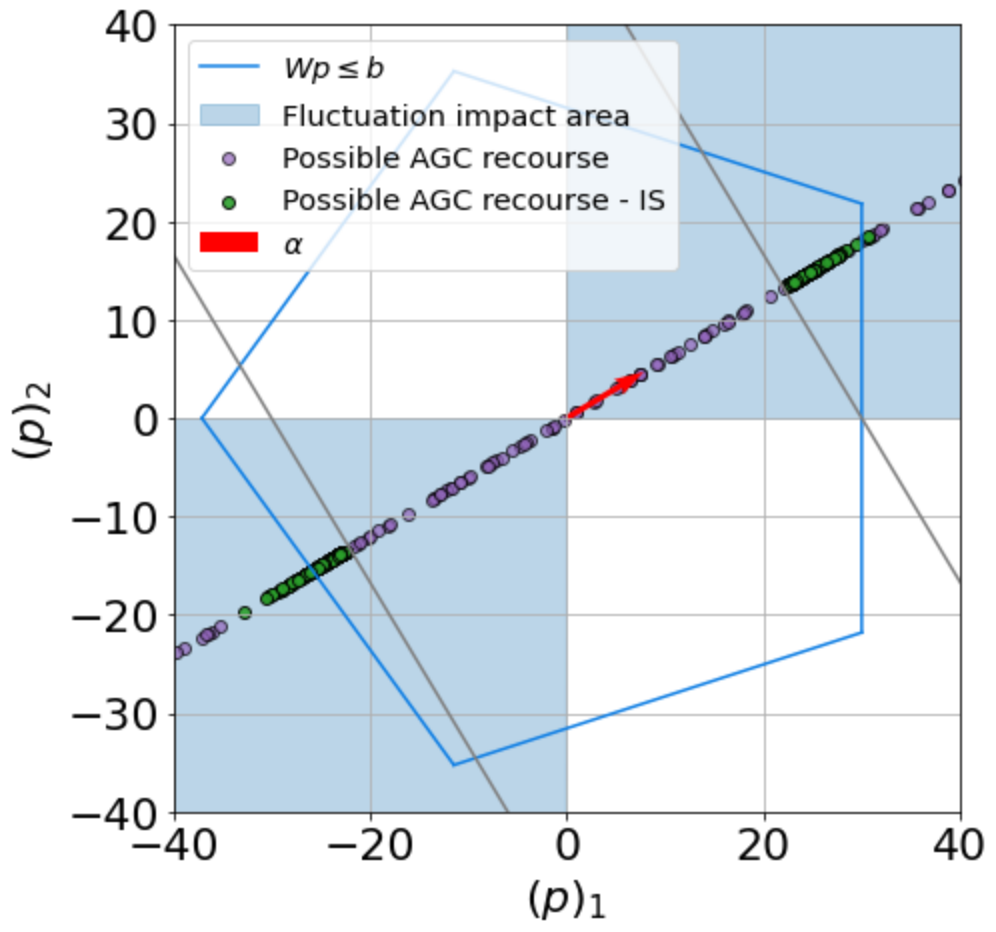
\includegraphics[width=.25\textwidth]{Dissertation/images/dynamic/poly_and_alpha_mc_vs_is.png}
%     \vspace{-5mm}
%     \caption{Realizations of AGC recourse from importance sampling are obtained such that are appear outside of the redundant samples set $\mathcal{P}_r$.
%     }
%     \label{fig:importance_sampled_vs_mc}
%     \vspace{-5mm}
% \end{figure}
 

% \subsection{Numerical Method}\label{sec:nm}
%\vspace{-1mm}
\section{Empirical Study}\label{sec:emp}
%\vspace{-1mm}
\subsection{Algorithms and Implementation Details}
%\vspace{-1mm}
We compare the performance of SA based on different strategies: classical Monte-Carlo (SA) and the proposed A-priori Reduced (AR-SA), and %. Moreover we compare the method proposed with 
the state-of-the-art scenario reduction methods: Fast-Forward, Simultaneous Backward \cite{heitsch2003scenario, dupavcova2003scenario} and K-Means \cite{keutchayan2023problem}. 
Data-Driven Chance Constrained Optimization over Wasserstein Balls (DD-DRO) from \cite{chen2024data}. 
For our test cases, we consider power systems from MATPOWER \cite{zimmerman2010matpower}, specifically Grid-6WW \cite{wood2013power} (pp. 104, 112, 119, 123-124, 549), Washington-14 and IEEE-30.
%
We implemented the algorithms using Python 3.9.13 and PandaPower 2.8.0 \cite{pandapower.2018} on a MacBook Pro (M1 MAX, 64 GB RAM). The optimization problems were solved using the Pyomo framework \cite{hart2017pyomo}
%and MindtPy \cite{bernal2018mixed}
, which employed GLPK \cite{Oki2012GLPKL}.% for mixed-integer programs and Ipopt \cite{wachter2006implementation} for non-linear subproblems. Without integer variables were present, MindtPy used only Ipopt. 
%The code is available on GitHub\footnote{https://github.com/vjugor1/OptimalControlScenarioApproximation}.
During the first case study, we reveal that DD-DRO, comparing with classical SA and proposed AR-SA, turns out to able to provide feasible solutions for JCC for fewer number of data samples. However, it is significantly heavier in terms of computation burden and less stable making this method less practical due to its internal complexity.
During the second case study, we compare AR-SA with classical SA and show significant (up to 2 times) improvements in the amount of data samples required to provide reliable solution.

We implemented the algorithms using Python 3.9.13 and PandaPower 2.8.0 \cite{pandapower.2018} on a MacBook Pro (M1 MAX, 64 GB RAM). For solving the optimization problem, we utilized Pyomo framework \cite{hart2017pyomo} and Mixed-Integer Nonlinear Decomposition Toolbox in Pyomo (MindtPy)   \cite{bernal2018mixed} optimization solver, which used GLPK \cite{Oki2012GLPKL} for internal mixed integer programs and Ipopt \cite{wachter2006implementation} for internal non-linear subproblems. MindyPy automatically detects if the problem provided does not have integer variables (SA and AR-SA cases) and uses Ipopt solely. 
The code for this chapter is available on Github\footnote{https://github.com/vjugor1/OptimalControlScenarioApproximation}.
%\vspace{-4mm}
\subsection{Test Cases and Numerical Results}
%\vspace{-1mm}
We conducted three case studies to evaluate the performance of SA, AR-SA, and other scenario reduction methods under different scenarios.  The first study focuses on the Grid-6WW and Washington-14, comparing the number of samples $N$ needed to achieve the $1-\rho=0.99$ reliability of $1-\eta$ feasible solution among 5 methods. 
The second study analyzed IEEE-30 bus system, which consist of 30 buses. 
In this case, we compared the number of samples needed to achieve a solution reliability of $1-\rho=0.99$ and assessed the total execution time, including the scenario reduction step. We summarized the required number of samples in Table \ref{tab:summary_results}. The value of $1-\eta$ is given by out-of-sample Monte Carlo; the empirical reliability is given by averaging over $L=100$ independent CC-OPF problem instances, as described in Algorithm~\ref{alg:estimate_delta}.
%
In all case studies, we model power generation and consumption fluctuations with a standard deviation of 0.01 of their nominal values, increasing cumulatively for each temporal snapshot. Thus, we expressed fluctuations as $\xi^t \sim \mathcal{N}(0, (\tilde{\sigma_t}^2))$, where $\tilde{\sigma_t}^2 = \tilde{\sigma}_0^2 \cdot t$. Simulations were carried out over $T=3$ temporal snapshots.% for each test case.
The third one compares SA, AR-SA and DD-DRO on Grid-6WW by estimating produced solutions' reliability and execution time.
The evaluation between SA, AR-SA, DD-DRO aims at a comparison of the number of samples $N$ required to obtain a solution with a reliability of $1-\rho$ (feasible for Problem \eqref{eq:optimal_control_2} with prob. $1-\rho$) and total execution time. Since DD-DRO is solved via complex mixed-integer non-linear programming \cite{chen2024data}, it is important to compare execution time together with amount of data required.
The second case study seeks to compare AR-SA and classical SA in the number of samples $N$ required to obtain a solution with a reliability of $1-\rho$.% As explained in Section \ref{sec:chancecontrol}, $1 - \eta$ stands for the confidence threshold for linear constraints, and $1-\rho$ is the probability of the scenario approximation solution to be feasible for.

\paragraph{Evaluation methodology.}
To get an empirical estimation of the solution reliability $1-\hat{\rho}$, we independently construct $L=100$ different approximations for both  SA and reduced SA. Further, we shortname SA with scenarios reduced by FF, SB and K-Means and $\hat{\mathcal{P}}_r$ as SA-FF, SA-SB, SA-KMeans and AR-SA respectively. The data-driven approximation size $N$ starts with $3$ and increases until the corresponding scenario approximation problem reaches $1-\hat{\rho} > 0.99$. For each approximation, we obtain $L$ different solutions: $(x^*_N)_l, ~ l=1, \dots, L$. We estimate the confidence of each obtained solution by running a series of out-of-sample validations. We use $10^4$ Monte-Carlo samples of $\xi$ to estimate of JCC feasibility constraint $(\hat{\mathbb{P}}_N)_l$, $l=1, \dots, L$. Finally, the solution reliability is given by $1 - \hat{\rho}$. It represents the fraction of $L$ solutions $(x^*_N)_l$ such that $(\hat{\mathbb{P}}_N)_l \geq 1 - \eta$. 
Alg.~\ref{alg:estimate_delta} summarizes the sequence of steps.

\begin{algorithm}[ht]
\SetKwInOut{Input}{input}
\SetKwRepeat{Do}{do}{while}
% \SetKwInOut{Output}{output}
\caption{Reliability $1-\hat{\delta}$ -- an empirical estimate}\label{alg:estimate_delta}
\Input{$L$ -- number of trials, DC-OPF problem parameters, $\eta$ -- confidence level, $N_0$ -- initial size of scenario approximation, $N_{\max}$ -- maximal size of scenario approximation}
$N \gets N_0$\;
$\hat{ \boldsymbol \delta}$ -- storage for $\hat{\delta}_N$\;
\Do{$N \leq N_{\max}$}
{
     $C_N \gets 0$ -- feasibility counter\;
     $l \gets 1$\;
    \Do{$l \leq L$}{
        Obtain $(x^*_N)_l$ -- scenario approximation with $N$ samples (using SA-IS or SA) \;
        Estimate constraint satisfaction probability $(\hat{\mathbb{P}}_N)_l$ using Monte Carlo samples.\label{alg:estimate_delta:phat_N_l}\;
        \uIf{$(\hat{\mathbb{P}}_N)_l \geq 1 - \eta$}{
            $C_N \gets C_N +1$
        }
        }
    $1-\hat{\delta}_N \gets C_N / L$ -- fraction of trials turned out to be feasible \;
    Append $\hat{\delta}_N$ to $\hat{ \boldsymbol \delta}$ \;
    $n  \gets n + N_{\max}/ 10$\;
}
\Return $\hat{ \boldsymbol \delta}$
\end{algorithm}

\paragraph{Complexity and Execution Time}
In addition to solving the SA optimization problem of type \eqref{eq:optimal_control_sampling_02}, selecting scenarios requires computational effort. The complexity of standard Monte Carlo-based SA (denoted as SA) does not require scenario reduction, unlike other methods, which need additional computations.

The Fast Forward method adds scenarios one by one based on probabilistic metrics (2-Wasserstein distance) and redistributes probabilities after each addition. Simultaneous Backward, on the other hand, removes scenarios using the same process. Denoting $N_r$ as the target number of scenarios after reduction, the complexities of these methods are $O(N_r^3 + N_r N^2)$ and $O(N_r^3 + N^3)$, respectively \cite{heitsch2003scenario, rujeerapaiboon2022scenario}. The K-Means algorithm is based on iterative estimation of scenario cluster centers and requires estimation of $L_2$ distance between scenarios and cluster centers. This algorithm requires $O(N_rN^2)$ \cite{pakhira2014linear} operations. Contrary, in the proposed AR-SA the reduction step is conducted via checking if a current samples is within $\hat{\mathcal{P}}_r$, thus, the complexity is $O(N)$. The construction of $\hat{\mathcal{P}}_r$ itself grows linearly with the number of deterministic constraints under probability measure in JCC of \eqref{eq:optimal_control_2}. 

We analyze the implications of the computational complexity by measuring total execution time: reduction and solving corresponding reduced scenario approximation. We conducted this experiment on IEEE-30 grid with target JCC feasibility level of $1-\eta=0.99$. The results are shown in Figure \ref{fig:ieee30time}. Here one can observe that the execution time almost similar for all the reduction methods with classical Monte-Carlo SA, except SA-SB. This indicates that the scenario reduction is computationally cheap operation, in comparison with solving optimization problem. Also, this experiment supports the proposed method in tractability.

% We consider the grid constraints to be satisfied with probability $1-\eta = 0.9$. The parameters for DD-DRO are as follows: Wasserstein ball with radius $r_W = 10^{-3}$, maximum function relaxation constant $M = 10$. Such parameters are chosen as minimal for $\eta$ and maximal for $r_W$ as possible, since for smaller $\eta$ and larger $r_W$ feasibility set of the DD-DRO turned out to be empty which was reported by the solver. The latter hints on an excessive conservativeness of the DD-DRO approach. Within non-strict reliability setup ($\eta=0.1$) we compare three methods: DD-DRO, SA and proposed AR-SA. We used the same number of samples for these methods, DD-DRO was based on the same samples that were used for classical SA, since changing the removing samples as proposed for AR-SA ones changes the underlying distribution of data and corrupts ambiguity set of DD-DRO. We were solving the corresponding optimization problem for $L=100$ independently sampled datasets.
%
%Figures \ref{fig:grid6reliability} and \ref{fig:grid6time} compare the performance of three methods on reliability and execution time. From the first figure, one can observe that DD-DRO, even for 2 data samples is able to produce solution that is more reliable for the original JCC Problem \ref{eq:optimal_control_2}. However, the boxplots that were produced from the reliabilities of DD-DRO solution are significantly more spread than of the SA and AR-SA, indicating method's instability. Also, average execution time of DD-DRO is uniformly five times larger than those of SA and AR-SA. The latter is caused by the fact that the underlying problem is non-linear and contains binary variables. In addition, DD-DRO optimization problem requires to assign 2 variables (1 binary and 1 positive real) for each data sample. Specifically, for Grid-6WW case with $N=100$ data samples, DD-DRO has 205 variables with 100 binary among them and 16302 constraints. Meanwhile, SA and AR-SA have only 4 continuous variables and 16203 constraints. 
%
Having conducted this analysis, we continue with SA and AR-SA and other reduction methods on larger grids and more strict reliability ($\eta = 0.05, ~0.01$) requirements in JCC optimization problem \eqref{eq:optimal_control_2}.
\vspace{-1mm}
\paragraph{ SA Solution Reliability.}
\begin{table}[t]
\caption{The number of samples for AR-SA and SA required in CC-OPF with a confidence threshold of $1-\eta$ to get the empirical reliability of $1-\hat{\rho} = 0.99$. 
    }
    \centering
    % \adjustbox{width=\linewidth}{
        % \begin{tabular}{lrr|lr|ll}
        \begin{tabular}{|lr|rlrll|}
        \toprule
        Case & $\eta$ & SA & AR-SA & SA-FF & SA-SB & SA-KMeans \\
\midrule
grid14 & 0.05 & 93 & 48 & 48 & 138 & 48 \\
grid30 & 0.05 & 138 & 93 & 138 & 138 & 93 \\
grid14 & 0.01 & 363 & 93 & 363 & 363 & 363 \\
grid30 & 0.01 & 453 & 273 & 453 & 453 & 453 \\
\bottomrule
  % Case &  $\eta$ &  SA No &             SA Cost &  AR-SA No &          AR-SA Cost & DC-OPF Cost \\
  %       \midrule
  %           grid14 &    0.05 &     93 & 5.5e+03$\pm$1.2e-11 &        48 & 5.5e+03$\pm$5.5e-12 &     5.2e+03 \\
  %           grid30 &    0.05 &     273 & 6.0e+03$\pm$2.8e-11 &        93 & 6.3e+03$\pm$1.3e-11 &     5.7e+03 \\
  %           grid14 &    0.01 &    273 & 5.6e+03$\pm$1.5e-11 &        93 & 5.5e+03$\pm$1.5e-11 &     5.2e+03 \\
  %           grid30 &    0.01 &    363 & 6.2e+03$\pm$4.5e-12 &       183 & 6.1e+03$\pm$4.5e-12 &     5.7e+03 \\
  %           \bottomrule
        \end{tabular}
    % }
    \label{tab:summary_results}
\end{table}
Following this analysis, we evaluate methods on larger grids with high reliability requirements. % ($\eta = 0.05, ~0.01$) for the JCC optimization problem \eqref{eq:optimal_control_2}.
%We analyse of numerical performance of classical SA and proposed AR-SA in more details over large test cases. 
This experiment seeks to find the number of samples sufficient for a solution of data-driven approximation to be feasible for original JCC with high probability for different $\eta$.
We estimate the number of samples required to reach confidence thresholds of $1-\eta = 0.95$ and $0.99$ with reliability of $0.99$ for AR-SA, SA, SA-FF, SA-SB and SA-KMeans in Table~\ref{tab:summary_results}, showing the number of samples required is 30-50\% less for AR-SA compared to classical SA and the advantage of AR-SA increases with the increase of $1-\eta$.

\begin{figure}[hbt]
    \centering
    \begin{subfigure}{.9\textwidth}
      \centering
      % include second image
      \hspace{-0mm}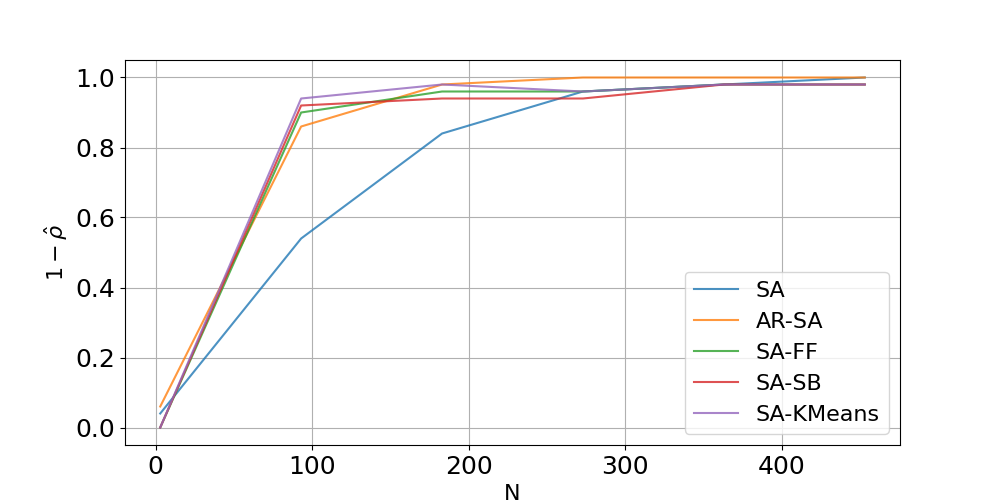
\includegraphics[width=0.99\linewidth]{Dissertation/images/dynamic/ieee30/1_beta_N_453_eta_0.01.png}
      \caption{Empirical reliability %($1-\hat{\rho}$) 
      vs $\#$ samples  in CC-OPF, $\eta = 0.01$.}
      \label{fig:ieee30conservatism}
    \end{subfigure}\\
        
    \begin{subfigure}{.9\textwidth}
      \centering
\hspace{10mm}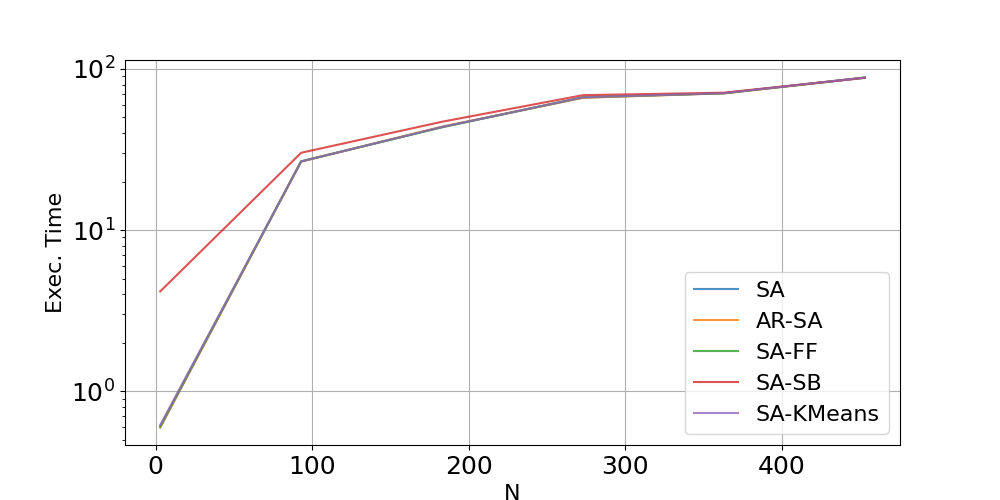
\includegraphics[width=0.99\linewidth]{Dissertation/images/dynamic/ieee30/exec_time_N_453_eta_0.01.png}~~~~~~\hfill
      \caption{Exec. time vs $\#$ samples, $\eta = 0.01$.
      }
      \label{fig:ieee30time}
    \end{subfigure}
    \caption{Numerical comparison of execution time and the reliability of reduced approximations' solution on IEEE 30 bus system.  
    }
\label{fig:ar-sa-ieee30}
\end{figure}

\begin{figure}[hbt]
    \centering
    \begin{subfigure}{.9\textwidth}
      \centering
      % include second image
      \hspace{-0mm}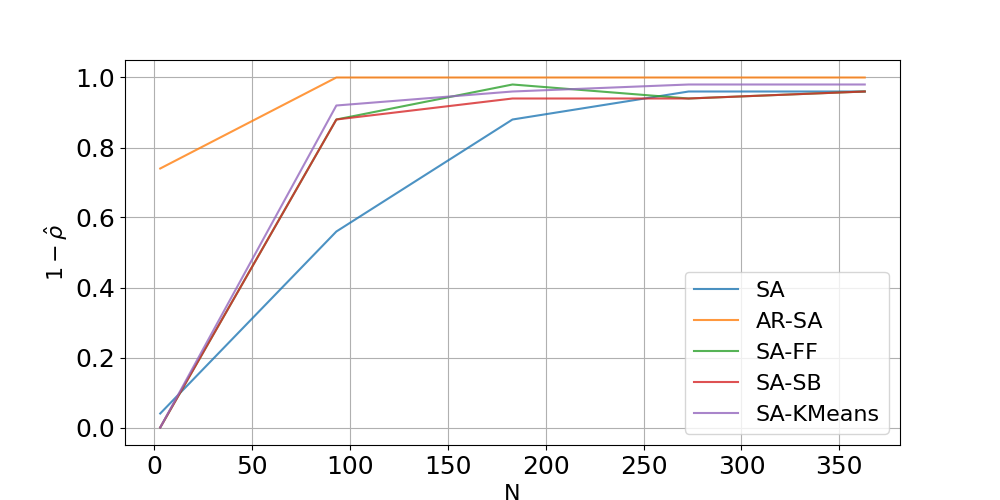
\includegraphics[width=0.99\linewidth]{Dissertation/images/dynamic/washington14/1_beta_N_363_eta_0.01.png}
      \caption{Washington 14 bus, $\eta = 0.01$.}
      \label{fig:washington14conservatism}
    \end{subfigure}
    
    \begin{subfigure}{.9\textwidth}
      \centering
      % include second image
      \hspace{0mm}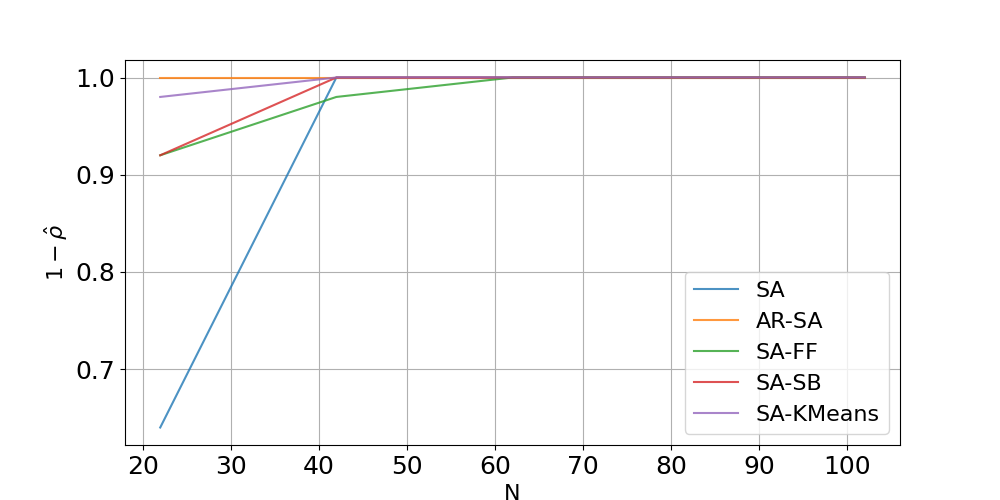
\includegraphics[width=0.99\linewidth]{Dissertation/images/dynamic/grid6/1_beta_N_102_eta_0.1.png}
      \caption{Grid6-WW 6 bus system, $\eta = 0.1$.}
      \label{fig:grid6reliability}
    \end{subfigure}
    \caption{Numerical comparison of reduced approximations' solution: empirical reliability ($1-\hat{\rho}$) vs $\#$ samples for CC-OPF.  
    }
\label{fig:ar-sa-wash14-grid6}
\end{figure}

\begin{figure}[hbt]
    \centering
    \begin{subfigure}{.9\textwidth}
      \centering
      % include second image
      \hspace{0mm}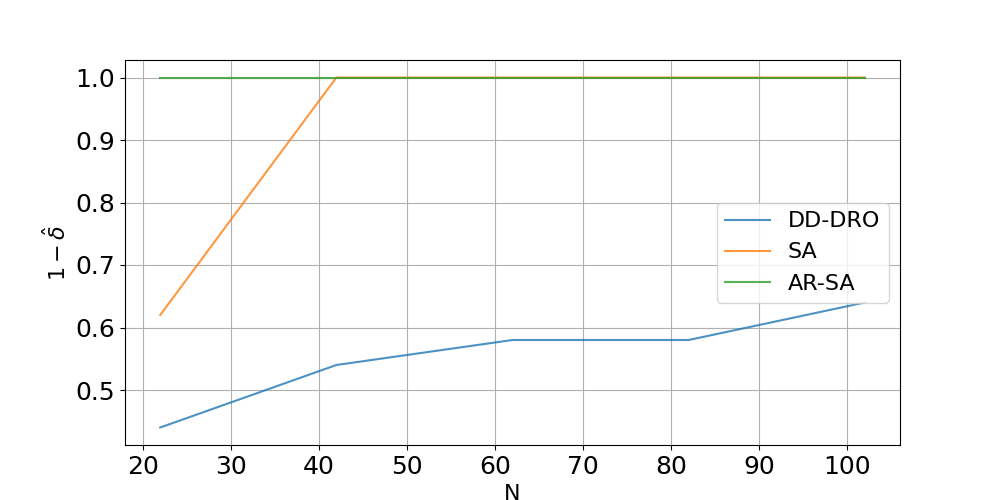
\includegraphics[width=0.99\linewidth]{Dissertation/images/dynamic/grid6/dd-dro/1_beta_N_102_eta_0.1.png}
      \hspace{0mm}\caption{Empirical reliability %($1-\hat{\rho}$) 
      vs $\#$ samples in CC-OPF, $\eta = 0.1$.}
      \label{fig:grid6reliability-dd-dro}
    \end{subfigure}
    
    \begin{subfigure}{.9\textwidth}
      \centering \hspace{10mm}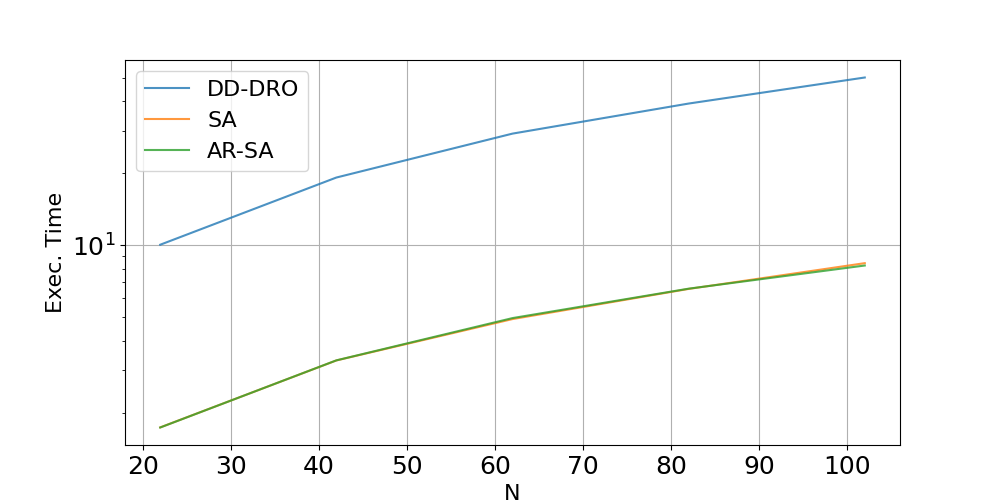
\includegraphics[width=0.99\linewidth]{Dissertation/images/dynamic/grid6/dd-dro/exec_time_N_102_eta_0.1.png}~~~~~~\hfill
      \caption{Exec. time vs $\#$ samples, $\eta = 0.1$.
      }
      \label{fig:grid6time-dd-dro}
    \end{subfigure}
    \caption{Numerical comparison of execution time and the reliability between classical MC based SA, AR-SA and DD-DRO on Grid6-WW 6 bus system.  
    }
\label{fig:ar-sa-vs-dd-dro}
\end{figure}

\begin{comment}
\begin{figure*}[hbt]
\vspace{-3mm}
\vspace{-3mm}
% \begin{subfigure}{.5\textwidth}
%   \centering
%   % include second image
%   \hspace{-1mm}\includegraphics[width=\linewidth]{Dissertation/images/dynamic/ieee57/1_beta_N_633_eta_0.01.png}
%   \caption{Empirical reliability $(1-\hat{\rho})$ versus the number of samples $N$\\ in CC-OPF for IEEE 57 bus system, $\eta = 0.01$.}
%   \label{fig:ieee57conservatism}
% \end{subfigure}
% \begin{subfigure}{.5\textwidth}
%   \centering
%   % include first image
%   \includegraphics[width=\linewidth]{Dissertation/images/dynamic/ieee57/boxplot_J_N_633_eta_0.01.png}~~~~~~\hfill
%   \caption{Spread of the probability of constraint feasibility, $(\hat{\mathbb{P}}_N)_l$, versus number of samples $N$ in CC-OPF for IEEE 57 bus system, $\eta = 0.01$.}
%   \label{fig:ieee57reliability}
% \end{subfigure}
\begin{subfigure}{.5\textwidth}
  \centering
  % include second image
  \hspace{-1mm}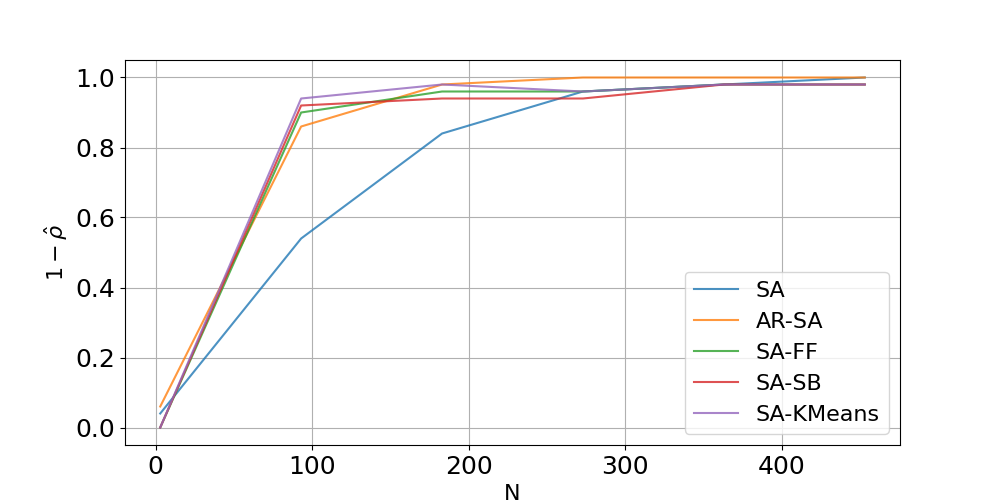
\includegraphics[width=\linewidth]{Dissertation/images/dynamic/ieee30/1_beta_N_453_eta_0.01.png}
  \caption{Empirical reliability ($1-\hat{\rho}$) versus number of samples $N$ \\ in CC-OPF for IEEE 30 bus system, $\eta = 0.01$.}
  \label{fig:ieee30conservatism}
\end{subfigure}
\begin{subfigure}{.5\textwidth}
  \centering
  % include first image
  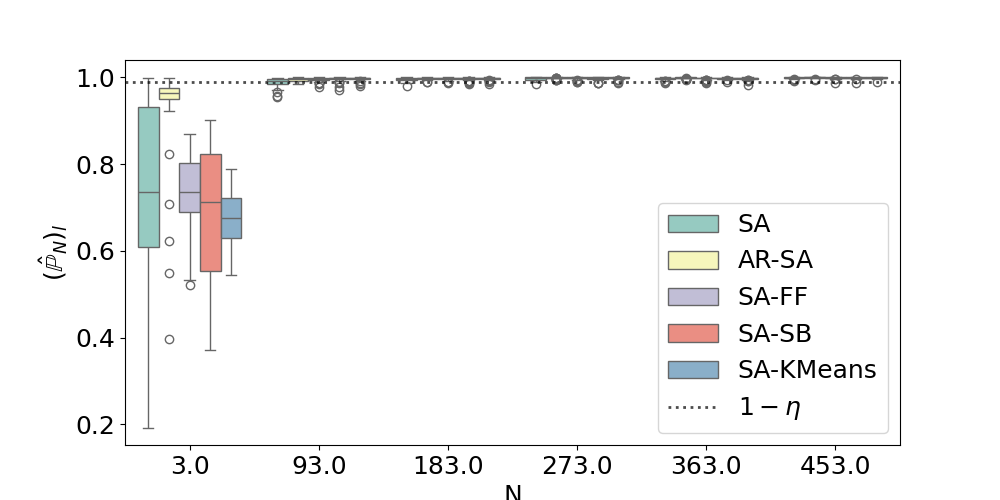
\includegraphics[width=\linewidth]{Dissertation/images/dynamic/ieee30/boxplot_J_N_453_eta_0.01.png}~~~~~~\hfill
  \caption{Spread of the probability of constraint feasibility, $(\hat{\mathbb{P}}_N)_l$, versus the number $N$  of samples in CC-OPF for IEEE 30 bus system, $\eta = 0.01$.}
  \label{fig:ieee30reliability}
\end{subfigure}
% \begin{subfigure}{.5\textwidth}
%   \centering
%   % include second image
%   \hspace{-1mm}\includegraphics[width=\linewidth]{Dissertation/images/dynamic/washington14/1_beta_N_633_eta_0.01.png}
%   \caption{Empirical reliability ($1-\hat{\rho}$) versus number of samples $N$ \\ in CC-OPF for Washington 14 bus system, $\eta = 0.01$.\\}
%   \label{fig:washington14conservatism}
% \end{subfigure}
% \begin{subfigure}{.5\textwidth}
%   \centering
%   % include first image
%   \includegraphics[width=\linewidth]{Dissertation/images/dynamic/washington14/boxplot_J_N_633_eta_0.01.png}~~~~~~\hfill
%   \caption{Spread of the probability of constraint feasibility, $(\hat{\mathbb{P}}_N)_l$, versus the number $N$ of samples in CC-OPF for the Washington case, $\eta = 0.01$.}
%   \label{fig:washington14reliability}
% \end{subfigure}
\vspace{-2mm}
\caption{(a) Empirical reliability ($1-\hat{\rho}$) and (b) The spread of constraint feasibility $(\hat{\mathbb{P}}_N)_l$ for CC-OPF ($1-\eta =.99$) in IEEE 57 \& 30 bus, the Washington 14 resp. system. The three cases correspond to samples in CC-OPF drawn from SA and AR-SA. The empirical estimates are computed with $L = 200$ optimization instances (for $1-\hat{\rho}$), and $N_{MC}=10^4$ Monte-Carlo samples for each instance to determine constraint validation (for box-plot of $(\hat{\mathbb{P}}_N)_l$), as described in Algorithm~\ref{alg:estimate_delta}. 
Colored boxes stand for the 25\% -- 75\% interquartile range (IQR). Diamonds show samples outside of the $\pm 1.5*\text{IQR}$. 
Note that both in reliability and the IRQ of constraint feasibility, AR-SA requires much less number of samples compared to SA or~SA-O.}
\label{fig:ieee118}
\end{figure*}
\end{comment}
%To better illustrate the dependency between number of samples in the approximation $N$ and relibaility estimates $1 - \hat{\rho}$, we demonstrate Figure \ref{fig:ieee30reliability}.
We illustrate the dependence between empirical reliability, $1-\hat{\rho}$, and the number of samples, $N$, for different values across the IEEE-30, Washington-14 and Grid6-WW systems in Figures \ref{fig:ar-sa-wash14-grid6} and \ref{fig:ar-sa-wash14-grid6}. Here, Figures \ref{fig:ieee30conservatism}, \ref{fig:washington14conservatism}, \ref{fig:grid6reliability} illustrate empirical reliability ($1-\hat{\rho}$), meanwhile Figures \ref{fig:ieee30time}, \ref{fig:grid6time-dd-dro} -- Execution time for various power grid test cases. The empirical estimates are computed with $L = 100$ optimization instances (for $1-\hat{\rho}$), and $N_{MC}=10^4$ Monte-Carlo samples for each instance to determine constraint validation (for box-plot of $(\hat{\mathbb{P}}_N)_l$), as described in Algorithm~\ref{alg:estimate_delta}. We maintain a confidence threshold for JCC feasibility of $1-\eta = 0.99$. 
Also, we present box plots showing the spread of $(\hat{\mathbb{P}}_N)_l$—the empirically computed probability of constraint satisfaction using $10^4$ Monte Carlo samples as per Algorithm \ref{alg:estimate_delta}, see Eq.~\ref{alg:estimate_delta:phat_N_l}. 
Notably, AR-SA achieves higher reliability levels ($1-\hat{\rho}$) with significantly fewer samples $N$. From Figures \ref{fig:ieee30conservatism},  \ref{fig:washington14conservatism} and \ref{fig:grid6reliability} one can observe that for Washington-14 and Grid6-WW AR-SA reaches high reliability levels with a lower number of samples and in IEEE-30 case, though SA, SA-FF, SA-SB, and SA-KMeans reach $1 - \rho = 0.9$ with less samples, the higher $1 - \rho =0.99$ reliability level is reached by AR-SA first. This observation is due to the problem-specific redundancy set $\hat{\mathcal{P}}_r$ construction that is able to filter specifically those scenarios that are irrelevant for the given problem.

\paragraph{AR-SA and DD-DRO comparison.}
We assessed grid constraints to be met with a probability of $1-\eta = 0.9$. For DD-DRO, we set the parameters as follows: a Wasserstein ball radius of $r_W = 10^{-3}$ and a maximum function relaxation constant of $M = 10$. These parameters were selected to be minimally conservative for $\eta$ and maximally expansive for $r_W$, as smaller $\eta$ values and larger $r_W$ values led to an empty feasibility set, indicating excessive conservativeness of DD-DRO. In a non-strict reliability setup ($\eta=0.1$), we compared DD-DRO, SA, and the proposed AR-SA using an identical number of samples. For DD-DRO, we use the same sample set as for classical SA to prevent changes in the underlying data distribution that would affect the ambiguity set of DD-DRO when adopting the sample reduction strategy for AR-SA. Figures \ref{fig:grid6reliability-dd-dro} and \ref{fig:grid6time-dd-dro} illustrate the performance differences in reliability and execution time across methods. Notably, DD-DRO achieved higher reliability for the JCC Problem \eqref{eq:optimal_control_2} even with just two data samples. But, its reliability boxplots were significantly more spread than those of SA and AR-SA, indicating instability. The average run time for DD-DRO is consistently 5x longer than that for SA and AR-SA, owing to the non-linear nature of the problem and the inclusion of binary variables. Indeed, in the Grid-6WW case with $N=100$ data samples, DD-DRO handle 205 variables, including 100 binary, and 16,302 constraints, while SA and AR-SA use only 4 continuous variables and 16,203 constraints.
%The box plots reveal that AR-SA rapidly reduces the variance in the solutions’ chance-constraint feasibility, characterized by thinner box plots and fewer outliers, compared to SA.
%We illustrate the dependence between empirical reliability $1-\hat{\rho}$ and $N$ over a range of values for the IEEE-30 (Washington-14) bus system in Fig.~ \ref{fig:ieee30reliability} (\ref{fig:washington14reliability}). Here, we keep a confidence threshold of joint chance constraint feasibility $1-\eta =0.99$. Moreover, we present box-plots for the spread of $(\hat{\mathbb{P}}_N)_l$ for different $N$, in Fig.~\ref{fig:ieee30conservatism} (\ref{fig:washington14conservatism}). We denote $(\hat{\mathbb{P}}_N)_l$ as the probability of constraint satisfaction, empirically computed using $10^4$ Monte Carlo samples of Algorithm \ref{alg:estimate_delta}, see Eq.~\ref{alg:estimate_delta:phat_N_l}. Note that AR-SA reaches a higher reliability level ($1-\hat{\rho}$) with a substantially fewer number of samples $N$. These boxplots indicate that the variance in the obtained solution's chance-constraint feasibility reduces faster for AR-SA, noted by thinner boxplots and lack of outliers, compared to SA.
%\vspace{-3mm}
%\begin{figure}[!ht]
    %\centering
    %\vspace{-3mm}
    %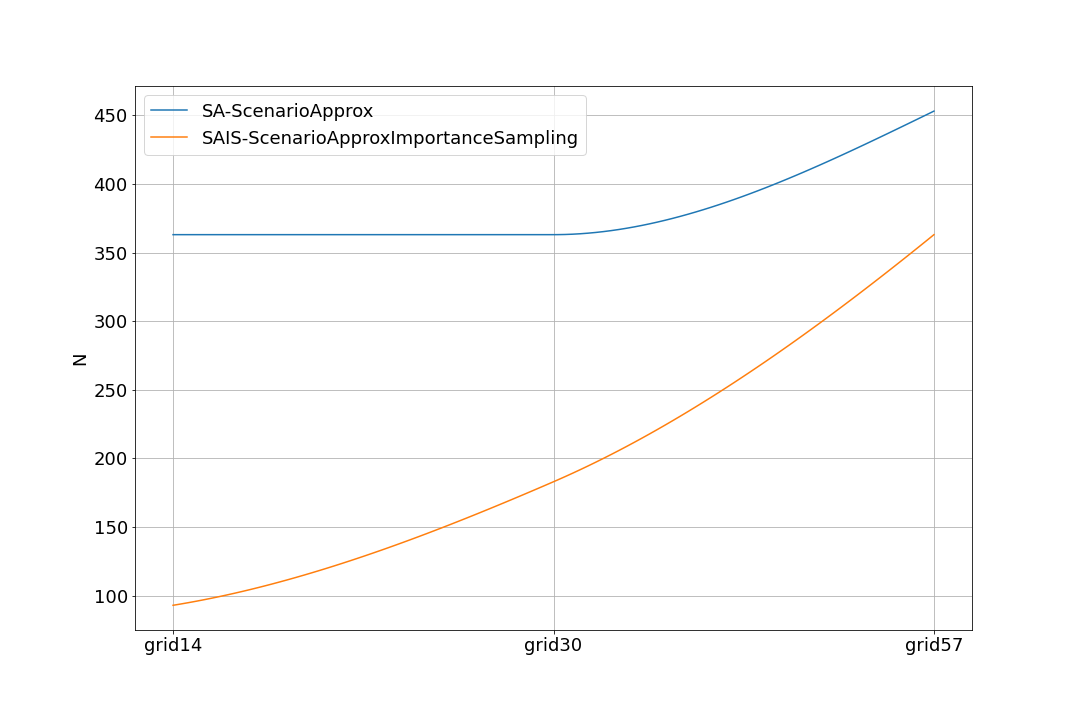
\includegraphics[width=.45\textwidth]{Dissertation/images/dynamic/summary_plot_001.png}
%    \vspace{-5mm}
%    \caption{Number of samples required to reach $0.99$ reliability level depending on the grid case.
%    }
%    \label{fig:summary grid 001}
    %\vspace{-5mm}
%\end{figure}

%Figure~\ref{fig:summary grid 001} illustrates the superior sample efficiency of AR-SA.
% \vspace{-1mm}
\section{Conclusion}\label{sec:conclusion}
% \vspace{-1mm}
Data-driven approximations are useful in chance-constrained stochastic programs with unknown uncertainty distribution and/or JCC settings. However, the data requirements rapidly become infeasible with the increase in size and reliability requirements. To address this, we proposed a novel approach that allows us to a-priorily identify and remove redundant scenarios in stochastic approximations for JCC dynamic multi-timestamp DC-OPF. We prove the validity of this approach theoretically and 
ensured its high empirical performance over various test cases. 
\addcontentsline{toc}{chapter}{Conclusions}
\chapter*{Conclusion}


%1. Restate the Research Problem and Objectives
%Begin by briefly restating the research problem and the primary objectives of your thesis. This reminds readers of the central focus of your work.

% Example:
% "In this thesis, we addressed the challenge of integrating renewable energy sources into power systems, with a focus on improving reliability and optimizing power flow under uncertainty. Our primary objectives were to develop advanced methods for reliability assessment and to propose novel optimization techniques for chance-constrained optimal power flow."

In this thesis, we addressed the the challenges that occur in modeling power systems that experience high level of renewable energy penetration. Our main objective was to develop advanced statistical methods for current operating point reliability assessment and to propose novel optimization techniques for chance-constrained optimal power flow in various settings.

% 2. Summarize Key Findings
% Summarize the key findings and contributions of your research. Highlight the most important results and how they address the research problem.

% Example:
% "Our research led to the development of an adaptive importance sampling method, which significantly improves the accuracy and efficiency of risk estimation for reliability constraints. Additionally, the proposed A-priori Reduced Scenario Approximation (AR-SA) method reduces the number of samples required for reliable solutions in joint chance-constrained dynamic optimal power flow problems. These methods were validated through extensive simulations, demonstrating their effectiveness in handling uncertainties in power systems."

This research led to the development of adaptive importance sampling methods for grid reliability estimation and proposed new techniques for constructing scenario approximation for static and dynamic formulation of optimal power flow.

% 3. Discuss the Significance and Impact
% Discuss the broader significance and impact of your findings. Explain how your research contributes to the field and its potential real-world applications.

% Example:
% "The findings of this thesis have significant implications for the integration of renewable energy sources into power systems. By enhancing the reliability and efficiency of power system operations, our methods support the transition to sustainable energy solutions, contributing to global efforts to reduce greenhouse gas emissions and improve energy security. Furthermore, the proposed techniques can be applied to other areas of power systems engineering, offering a foundation for future advancements in the field."

The findings have significant implications on computing and estimating generation regimes of power grids, allowing for non-restrictive robust, statistical based calculation of generation regimes and efficient estimation of the latter's reliability. This contributes to safer transition to sustainable energy solutions, contributing to global efforts to reduce greenhouse gas emissions and improve energy security. Furthermore, the proposed techniques can be applied to other areas of power systems engineering and beyond, where uncertainty arises in optimization problems, offering a foundation for future advancements in the field.

% 4. Address Limitations
% Acknowledge any limitations of your research. Being transparent about the constraints and challenges you encountered adds credibility to your work.

% Example:
% "While our methods offer substantial improvements, there are limitations to consider. The adaptive importance sampling method relies on accurate physical information, which may not always be readily available. Additionally, the computational complexity of the AR-SA method, though reduced, may still pose challenges for extremely large-scale power systems."

Though the methods offer substantial improvements, there are limitations to consider. The method rely on high-voltage assumption, leading to a linear system/problems. However, the results can be generalized for non-linear cases by additional mathematical effort.

% 5. Suggest Future Work
% Suggest directions for future research based on your findings. Identify areas that require further investigation and how they can build on your work.

% Example:
% "Future research could explore the application of the adaptive importance sampling method to real-time power system operations, addressing the challenge of obtaining real-time physical data. Further development of the AR-SA method could focus on enhancing its scalability and applicability to even larger power grids. Additionally, integrating these methods with emerging technologies, such as smart grid systems and advanced forecasting techniques, presents a promising avenue for future work."

Future research could explore applications for non-linear settings and broader distribution class support. The former could be achieved by iterative constructions of convex restrictions and the latter with distributionally robust optimization techniques. 

% 6. Final Thoughts
% Conclude with a few final thoughts that encapsulate the essence of your research and its potential to inspire further advancements in the field.

% Example:
% "In conclusion, this thesis contributes to the ongoing efforts to integrate renewable energy sources into power systems more effectively. The developed methods not only address current challenges but also pave the way for future innovations. As the global energy landscape continues to evolve, the insights gained from this research will be instrumental in shaping a sustainable and resilient energy future."

In conclusion, this thesis contributes to the ongoing efforts to integrate renewable energy sources into power systems more effectively. The developed methods not only address current challenges but also pave the way for future innovations. As the global energy landscape continues to evolve, the insights gained from this research will be instrumental in shaping a sustainable and resilient energy future.



% \newpage
% % \addcontentsline{toc}{chapter}{List of figures}
% \listoffigures

% % \addcontentsline{toc}{chapter}{List of tables}
% \listoftables      % Заключение
% \printnomenclature[3.5cm] % Значение ширины столбца с обозначениями стоит подбирать вручную


\addcontentsline{toc}{chapter}{List of symbols and abbreviations}
\chapter*{List of symbols and abbreviations}

\begin{tabularx}{0.9\textwidth}{lX}
	AD & Anomaly Detection \\
	AUROC & Area Under Receiver Operating Characteristic (Curve) \\
	BCE & Binary Cross-Entropy \\
	BGP & Burdenko’s Glioblastoma Progression \\
	BN & Batch Normalization \\
	CE & Contrast Enhancement \\
	CNN & Convolutional Neural Network \\
	COVID-19 & Coronavirus Disease 2019 \\
	CT & Computer Tomography \\
	DA & Domain Adaptation \\
	DANN & Domain Adversarial Neural Network \\
	DL & Deep Learning \\
	DNN & Deep Neural Network \\
	DSC & Dice Similarity Coefficient \\
	FBP & Filtered Back-Projection \\
	% FDA & Fourier Domain Adaptation \\
	FPR & False-Positive Rate \\
	GAN & Generative Adversarial Network \\
	GGO & Ground-Glass Opasity \\
	GTV & Gross Tumor Volume \\
	HM & Histogram Matching \\
	HU & Hounsfield Units \\
	ID & In-Distribution \\
	IHF & Intensity Histogram Features \\
	IN & Instance Normalization \\
	LDCT & Low Dose Computer Tomography \\
	MCD & Monte-Carlo Dropout \\
	MRI & Magnetic Resonance Imaging \\
	MSE & Mean Squared Error \\
	NN & Neural Network \\
	OOD & Out-of-Distribution \\
	PCA & Principal Component Analysis \\
	ROI & Region of Interest \\
	
	
	 %%%%%%%%
	
%    $I$ & Identity matrix \\
%    $1$ & Vector of ones \\
%    $A^*$ & Complex conjugate of a matrix \\
%    $A^\top$ & Transpose of a matrix \\
%    $\|A\|_p$ & Operator $p$-norm of a linear operator, $2$-norm of a linear operator if not specified \\
%    $\mathbbm{C}$ & The field of complex numbers \\
    
%    $\mathbb{P}$ & Probability measure \\
%    $\mathbb{E}$ & Mathematical expectation \\
%    $\mathbb{V}$ & Variance \\
%    $\textup{KL}$ & Kullback-Leibler divergence \\
%    $\mathcal{N}(\mu, \Sigma)$ & Gaussian distribution with mean vector $\mu$ and covariance matrix $\Sigma$\\
%    $1\left[A\right]$ & Indicator of the event $A$ \\
%    $\rmi$ & Imaginary unit \\
%    $\nabla $ & Nabla operator \\
%    $\Phi(\cdot)$ & Cumulative Distribution Function (CDF) of the standard Gaussian distribution\\
\end{tabularx}

\begin{tabularx}{0.9\textwidth}{lX}
	SDA & Supervised Domain Adaptation \\
	% SE & Self-Ensembling \\
	SGD & Stochastic Gradient Descent \\
	SVD & Singular Value Decomposition \\
	T & Tesla, unit of magnetic flux density \\
	TPR & True-Positive Rate \\
	TL & Transfer Learning \\
	UDA & Unsupervised Domain Adaptation \\
	UE & Uncertainty Estimation \\
	$\R$ & The field of real numbers \\
	$\mathcal{F}\left[ \cdot \right]$ & Fourier transform of the input function \\
	$\kappa(t)$ & Ramp filter \\
	$\mathcal{R}\left( \cdot \right)$ & Radon transform of the input image \\
%    $I$ & Identity matrix \\
%    $1$ & Vector of ones \\
%    $A^*$ & Complex conjugate of a matrix \\
    $A^\top$ & Transpose of a matrix \\
    $\| \cdot \|_p$ & Operator $p$-norm of a tensor \\%, $2$-norm of a linear operator if not specified \\
%    $\mathbbm{C}$ & The field of complex numbers \\
%    $\mathbb{P}$ & Probability measure \\
%    $\mathbb{E}$ & Mathematical expectation \\
%    $\mathbb{V}$ & Variance \\
%    $\textup{KL}$ & Kullback-Leibler divergence \\
%    $\mathcal{N}(\mu, \Sigma)$ & Gaussian distribution with mean vector $\mu$ and covariance matrix $\Sigma$\\
%    $1\left[A\right]$ & Indicator of the event $A$ \\
%    $\rmi$ & Imaginary unit \\
%    $\nabla $ & Nabla operator \\
%    $\Phi(\cdot)$ & Cumulative Distribution Function (CDF) of the standard Gaussian distribution\\
\end{tabularx}

%\item 
%\item FBPAug -- Filtered Back-Projection Augmentation
%\item 
%\item 

%\item         % Список сокращений и условных обозначений
% \chapter*{Словарь терминов}             % Заголовок
\addcontentsline{toc}{chapter}{Словарь терминов}  % Добавляем его в оглавление

\textbf{TeX} : Cистема компьютерной вёрстки, разработанная американским профессором информатики Дональдом Кнутом

\textbf{панграмма} : Короткий текст, использующий все или почти все буквы алфавита
      % Словарь терминов
\clearpage                                  % В том числе гарантирует, что список литературы в оглавлении будет с правильным номером страницы
\urlstyle{rm}                               % ссылки URL обычным шрифтом
\ifdefmacro{\microtypesetup}{\microtypesetup{protrusion=false}}{} % не рекомендуется применять пакет микротипографики к автоматически генерируемому списку литературы

% Подсчёт общего числа записей
%\printbibliography[env=counter, keyword=bibliofull, section=0, heading=nobibheading]

%\insertbibliofull                           % Подключаем Bib-базы: все статьи единым списком
\insertbiblioexternal                      % Подключаем Bib-базы: статьи, не являющиеся статьями автора по теме диссертации
\insertbiblioauthor                        % Подключаем Bib-базы: работы автора единым списком 
%\insertbiblioauthorgrouped                 % Подключаем Bib-базы: работы автора сгруппированные (ВАК, WoS, Scopus и т.д.)
\insertbiblioregistered


\printbibliography[env=counter, keyword=bibliofull, heading=nobibheading]


\ifdefmacro{\microtypesetup}{\microtypesetup{protrusion=true}}{}
\urlstyle{tt}                               % возвращаем установки шрифта ссылок URL      % Список литературы
\clearpage
\ifdefmacro{\microtypesetup}{\microtypesetup{protrusion=false}}{} % не рекомендуется применять пакет микротипографики к автоматически генерируемым спискам
\listoffigures  % Список изображений

%%% Список таблиц %%%
% (ГОСТ Р 7.0.11-2011, 5.3.10)
\clearpage
\listoftables   % Список таблиц
\ifdefmacro{\microtypesetup}{\microtypesetup{protrusion=true}}{}
\newpage           % Списки таблиц и изображений (иллюстративный материал)

\setcounter{totalchapter}{\value{chapter}} % Подсчёт количества глав

%%% Настройки для приложений
\appendix
% Оформление заголовков приложений ближе к ГОСТ:
\setlength{\midchapskip}{20pt}
\renewcommand*{\afterchapternum}{\par\nobreak\vskip \midchapskip}

\ifnumequal{\value{englishthesis}}{0}{
    \renewcommand\thechapter{\Asbuk{chapter}} % Чтобы приложения русскими буквами нумеровались
}{}

% %\chapter{M3DA datasets description}
%\label{app:m3da_datasets}
%
%
%Below we provide an extended description of datasets used in M3DA benchmark, download and usage examples are available in the published repository\footnote{\href{https://github.com/BorisShirokikh/M3DA}{https://github.com/BorisShirokikh/M3DA}}. Example 2D slices from every dataset for visual comparison between domains are given in Figure~\ref{fig:contours}. Summary of licenses and data access is given in Table~\ref{tab:supp_datasets}.
%
%\begin{table}[h]
	\centering
	\caption{Datasets licenses and independent source links.}
	
	\resizebox{\linewidth}{!}{%
		\begin{tabular}{@{}lcc@{}}
			\toprule
			\textbf{Dataset} & license & link to dataset \\
			\midrule
			BraTS \cite{brats} & CC BY 4.0  & \href{https://www.cancerimagingarchive.net/analysis-result/rsna-asnr-miccai-brats-2021/}{https://www.cancerimagingarchive.net/analysis-result/rsna-asnr-miccai-brats-2021/} \\
			
			CC359 \cite{cc359} & CC BY-ND 4.0 & \href{https://www.ccdataset.com/download}{https://www.ccdataset.com/download}  \\
			
			AMOS \cite{amos} & CC BY 4.0 & \href{https://zenodo.org/records/7262581}{https://zenodo.org/records/7262581} \\
			
			AMOS LDCT & CC BY 4.0 & \href{https://zenodo.org/records/13373720}{https://zenodo.org/records/13373720} \\
			
			LIDC \cite{lidc} & CC BY 3.0 & \href{https://www.cancerimagingarchive.net/collection/lidc-idri/}{https://www.cancerimagingarchive.net/collection/lidc-idri/}\\
			
			\bottomrule
		\end{tabular}
	}
	\label{tab:supp_datasets}
\end{table}
%
%
%\section{AMOS}
%
%The AMOS dataset \cite{amos} contains 500 CT and 100 MRI abdominal scans with the multi-organ segmentation task: liver, stomach, spleen, left and right kidneys, bladder, aorta, pancreas, inferior vena cava, duodenum, prostate/uterus, gallbladder, esophagus, left and right adrenals. As a largest available dataset for inter-modality segmentation, we employed it in MR$\ra$CT and CT$\ra$MR domain shift setups. 
%
%We used all 60 labeled MRIs as the \textit{source} set in MR$\ra$CT setup and the \textit{target test} set in CT$\ra$MR. Then, 200 unlabeled CTs and 40 unlabeled MRIs were used as the \textit{target train} sets for adaptation purposes in the MR$\ra$CT and CT$\ra$MR setups, respectively. The remaining 300 labeled CTs were evenly split in two groups: the first is a source set in CT$\ra$MR, and the second is a target test set in MR$\ra$CT.
%
%Furthermore, we used AMOS CT images to create one of the most clinically relevant domain shift setups -- difference in the radiation dose during scanning. 
%% In CT$\ra$LDCT, we employed the first group of 150 labeled CTs as a source set, 200 unlabeled CTs as a target train set, and the second group of 150 labeled CTs as a target test set. 
%For the LDCT domain, we simulated low radiation dose using the algorithm provided in \cite{ldct}, simulated data are available at \href{https://zenodo.org/records/13373720}{https://zenodo.org/records/13373720}.
%
%
%\section{BraTS}
%
%BraTS \cite{brats} is comprised of 2000 brain MRI cases, each consisting of four sequences: T1, T1c, T2, FLAIR, with a glioblastoma segmentation classes (3 foreground classes and background).  We only used 1251 cases with publicly available annotations and T1, T1c MRI sequences for T1 CE$\ra$T1 shift. Since sequences of the same case provide information about the same subject, we ensured source-target splits so that every case falls into exactly one fold and split cases with 50:25:25 ratio into source, target train, and target test folds.
%
%
%\section{CC359}
%
%The CC359 dataset \cite{cc359} contains 359 brain MR T1 images from three scanners, namely, GE, Philips (PH), and Siemens (SM), obtained using two magnetic field strength values, $1.5$ and $3.0$T. The dataset can be split into six domains defined by two different field strengths $\times$ three vendors, each with approximately 60 images, so it yields 30 possible domain adaptation pairs. 
%
%CC359 also offers three tasks: brain, hippocampus, and white matter, gray matter, and cerebrospinal fluid (WMGMCSF) segmentation. We ommited hippocampus segmentation task from the benchmark, because our preliminary experiments showed it is not significantly affected by domain shifts, the relative performance drop is less than $2\%$ in every domain pair; see Table~\ref{tab:hippo}. We also omitted the brain segmentation task for the same reason, see results in \cite{shirokikh2020first}.
%
%

\begin{table}[h]
	\centering
	\caption{Baseline and oracle results on the CC359 WMGMSCF segmentation task.}
	\label{tab:wmgmcsf}
	
	% \resizebox{\columnwidth}{!}{%
		\begin{tabular}{|c|l||c|c|c|c|c|c|}
			
			\hline
			\multicolumn{2}{|l||}{\multirow{2}{*}{}}  & \multicolumn{6}{c|}{Target domains}\\ 
			\cline{3-8}
			\multicolumn{2}{|l||}{} & GE1.5 & PH1.5 & SM1.5 & GE3.0 & PH3.0 & SM3.0\\ 
			\hline
			\hline
			
			% \clrtb
			
			\multirow{6}{*}{{\rotatebox[origin=c]{90}{Source domains}}}
			& GE 1.5 & 95.8 & 82.1 & 90.8 & 82.1 & 92.6 & 80.8 \\
			\cline{2-8}
			
			& PH 1.5 & 80.1 & 92.7 & 90.8 & 93.4 & \textbf{74.1} & 90.1 \\
			\cline{2-8}
			
			& SM 1.5 & 89.7 & 85.3 & 95.6 & 86.2 & 86.2 & 84.5 \\
			\cline{2-8}
			
			& GE 3.0 & 76.6 & 89.9 & 90.3 & 95.9 & 72.0 & 91.4 \\
			\cline{2-8}
			
			& PH 3.0 & 90.6 & 74.7 & 86.0 & 75.4 & 95.4 & \textbf{76.6} \\
			\cline{2-8}
			
			& SM 3.0 & \textbf{56.0} & 88.6 & 84.9 & 92.4 & 68.4 & 95.7 \\
			\hline
			
		\end{tabular}%}
\end{table}


\begin{table}[h]
	\centering
	\caption{Baseline and oracle results on the CC359 hippocampus segmentation task.}
	\label{tab:hippo}
			
	%\resizebox{\columnwidth}{!}{%
		\begin{tabular}{|c|l||c|c|c|c|c|c|} 
			\hline
			\multicolumn{2}{|l||}{\multirow{2}{*}{}}  & \multicolumn{6}{c|}{Target domains}\\ 
			\cline{3-8}
			\multicolumn{2}{|l||}{} & GE1.5 & PH1.5 & SM1.5 & GE3.0 & PH3.0 & SM3.0 \\ 
			\hline
			\hline
			
			% \clrtb
			
			\multirow{6}{*}{{\rotatebox[origin=c]{90}{Source domains}}}
			& GE 1.5 & 92.3 & 86.7 & 88.7 & 87.8 & 91.2 & 91.2 \\
			\cline{2-8}
			
			& PH 1.5 & 91.3 & 86.9 & 87.7 & 87.7 & 89.7 & 89.9 \\
			\cline{2-8}
			
			& SM 1.5 & 91.7 & 86.6 & 89.3 & 88.2 & 90.9 & 90.8 \\
			\cline{2-8}
			
			& GE 3.0 & 91.4 & 86.4 & 88.0 & 89.1 & 90.5 & 91.3 \\
			\cline{2-8}
			
			& PH 3.0 & 91.5 & 86.5 & 88.3 & 87.7 & 92.0 & 91.0 \\
			\cline{2-8}
			
			& SM 3.0 & 90.8 & 86.5 & 87.8 & 88.0 & 90.6 & 92.1 \\
			\hline
			
	\end{tabular}%}
\end{table}

%
%Therefore, we focus only on the WMGMCSF segmentation task in CC359: white matter, gray matter and cerebral spinal fluid segmentation classes and background. From 30 possible domain pairs, we selected three with the maximum performance drop, highlighted in \textbf{bold},  Table~\ref{tab:wmgmcsf}): changing field strength with a fixed scanner PH 1.5T $\ra$ PH 3.0T (drop from 95.4 to 74.1 Dice score), changing scanner with the fixed field strength PH 3.0T $\ra$ SM 3.0T (drop from 95.7 to 76.6), and changing both parameters SM 3.0T $\ra$ GE 1.5T (drop from 95.8 to 56.0). We denote them as T1 F, T1 Sc, and T1 Mix, respectively.
%
%
%\section{LIDC}
%
%LIDC \cite{lidc} is a multi-center collection of diagnostic and lung cancer screening thoracic CT scans with annotated lesions. It includes 1308 studies (of which 1018 include CT studies) from 1010 patients. Lung's nodules is one of the few clinical applications where both CE CT and CT are used, first for the initial scan, and second for the follow-ups \cite{purysko2016does}. We used LIDC for CE CT $\ra$ CT domain shift, we split data into three roughly equal groups, ommiting scans with empty masks: contrast enhanced CT (source domain) $X^s$, CT without contrast enhancement $X^t_{tr}$ (training part, target domain), and CT without contrast enhancement  $X^t_{ts}$ (test part, target domain). $X^t_{tr}$ and $X^t_{ts}$ were stratified by the number of lesions.
%
%
%\chapter{M3DA methods description}
%\label{app:m3da_methods}
%
%As mentioned above, we used an nnU-Net \cite{nnunet} backbone as segmentation network architecture in all methods. We preserved most of the nnU-Net training pipeline except for several methodological changes, which allow us to evaluate DA methods, such as AdaBN and InstanceNorm, separately and run the ablation studies. These changes along with the other training hyper-parameters are summarized in Table~\ref{tab:hyper}.
%
%Firstly, we replaced the default InstanceNorm with BatchNorm layers and removed test-time augmentation, so we can compare different normalizations and adaptive normalizations (AdaBN) and assess the unhindered impact of DA methods. Secondly, we reduced the patch size and number of the network features, so all experiments fit in a single 16 GB NVIDIA Tesla V100 and our benchmark remains economical. We set the number of epochs to 600 in all experiments, so that any method could complete its training in three days. All experiments were conducted on the Zhores supercomputer~\cite{zacharov2019zhores}.
%
%

\begin{table}[h]
	\centering
	\caption{Hyper-parameters.}
	\label{tab:hyper}
	%\resizebox{\linewidth}{!}{
		\begin{tabular}{lcc}
			\toprule 
			\textbf{hyper-parameter} & \textbf{nnUNet} & \textbf{U-Net (ours)}  \\ 
			\midrule
			architecture & auto & auto \\
			base features & 32 & 24 \\
			normalization & instance (IN) & batch (BN) \\
			batch size & 2 & 2 \\
			patch size & (160, 192, 64) & (160, 160, 64) \\
			epochs & 600 & 600 \\
			batches per epoch & 250 & 250 \\
			loss & Dice Loss + CE & Dice Loss + CE \\
			% loss masking based on intensity & \cmark & \xmark \\
			oversampling rate & 0.66 & 0.75 \\
			optimizer & SGD & SGD \\
			momentum & 0.99 & 0.99 \\
			weight decay & $3 \times 10^{-5}$  & $3 \times 10^{-5}$ \\
			initial learning rate & $10^{-2}$ & $10^{-2}$ \\
			learning rate schedule & poly decay & poly decay \\
			learning rate decay power & 0.9 & 0.9 \\
			test-time augmentation & \cmark & \xmark \\
			\bottomrule
	\end{tabular}%}
\end{table}

%
%Below, we provide DA methods implementation details:
%
%\paragraph{Histogram matching} uses the baseline training pipeline, except all image intensity histograms are equalized to an average histogram computed over the train set. 
%
%\paragraph{Gamma augmentation} also uses the baseline training pipeline, and we perform gamma correction with randomly selected $\gamma \sim U[0.5, 2]$ on every input image.
%
%\paragraph{nnAugm} similarly supplements the same baseline training with the original set of nnUNet \cite{nnunet} augmentations.
%
%\paragraph{InstanceNorm} substitutes BN layers, while the training pipeline remains the same as in baseline.
%
%\paragraph{Adaptive BN} performs additional 1000 inference steps with batch size 4 over the baseline, updating the running statistics of BN layers on target training data.
%
%\paragraph{Self-ensembling} design and all parameters are reproduced from \cite{se_medim} with our architecture.
%
%\paragraph{MinEnt} adds a predictions entropy minimization criterion on target images. So we extended our training pipeline with the second step using target train images, and added entropy loss with the recommended in \cite{entropy} weight $\lambda = 0.001$.
%
%\paragraph{DANN} introduces an auxiliary network called discriminator. Similar to recent studies \cite{entropy}, we used DCGAN~\cite{dcgan} discriminator architecture, replacing 2D convolutions with 3D ones. The losses weighting parameter is taken from \cite{dann_medim}, e.g., $\alpha = 0.01$.
%
%\paragraph{CycleGAN 2D} is fully reused from the original study \cite{cyclegan}. We trained a standalone CycleGAN 2D to map between source and target train images, where we sample axial slices from our volumetric images and rescale them into 256 $\times$ 256 gray scale images. Before predicting with the baseline segmentation model, we applied one of the generators to target test images (slice-by-slice) to transform them into fake source ones.
%
%\paragraph{CycleGAN 3D} is fully reused from the original study \cite{cyclegan3d}. We trained a standalone CycleGAN 3D to map between source and target train images, where we sample patches of size (128, 128, 96) from our volumetric images. Before predicting with the baseline segmentation model, we applied one of the generators to target test images (via overlapping grid) to transform them into fake source ones.
%
%\paragraph{GIN} is fully reused from \cite{gin} with the implementation based on the nnU-Net framework.
%
%\paragraph{MIND} is fully reused from \cite{dg_tta} with the implementation based on the nnUNet framework.\\
%
%
%All experiments are available at \href{https://github.com/BorisShirokikh/M3DA-exp}{github.com/BorisShirokikh/M3DA-exp}.


%\chapter{Evidence of Industrial Application}
%\label{app:m3da_datasets}
\chapter{Certificate of Registration}
\label{app:reg}

\begin{center}
	%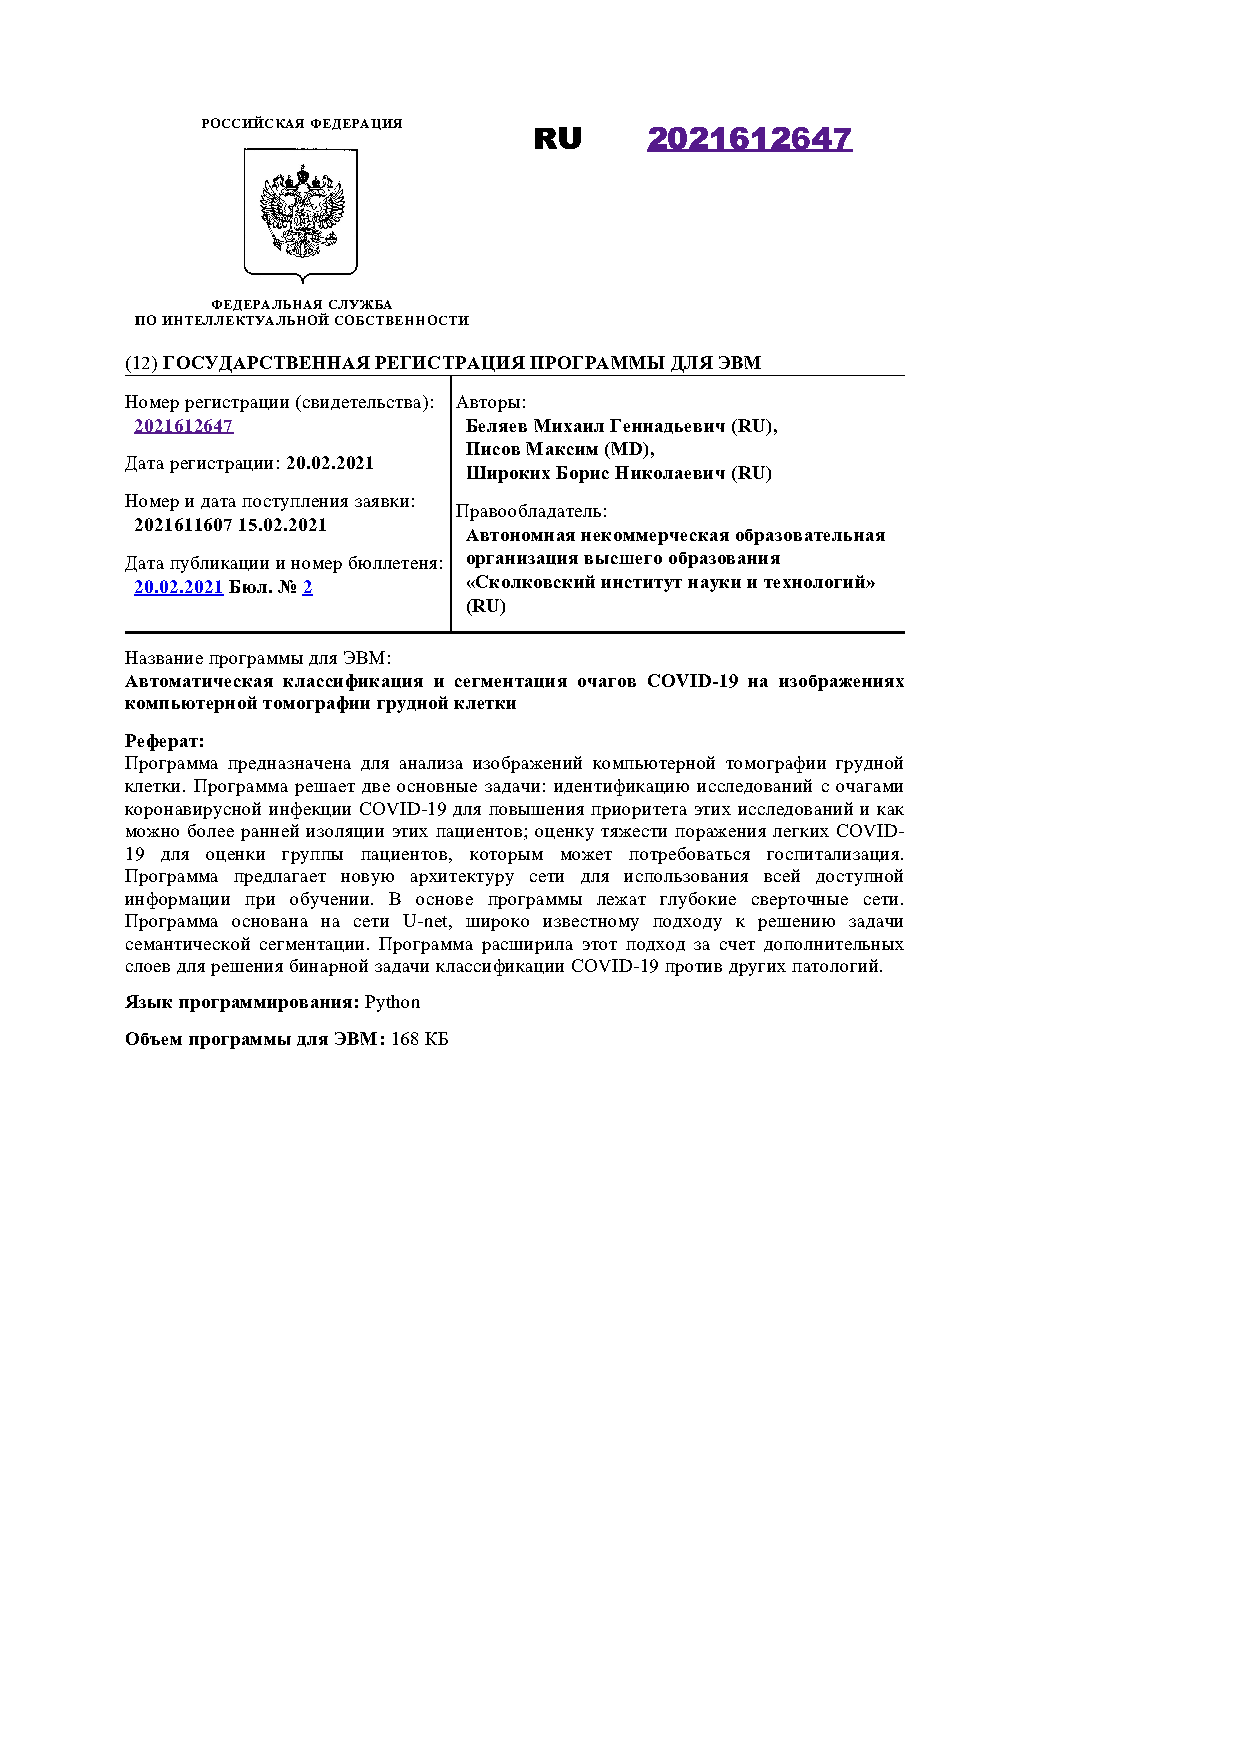
\includegraphics[width=\textwidth]{Dissertation/Figures/6_appendix/output.pdf}
	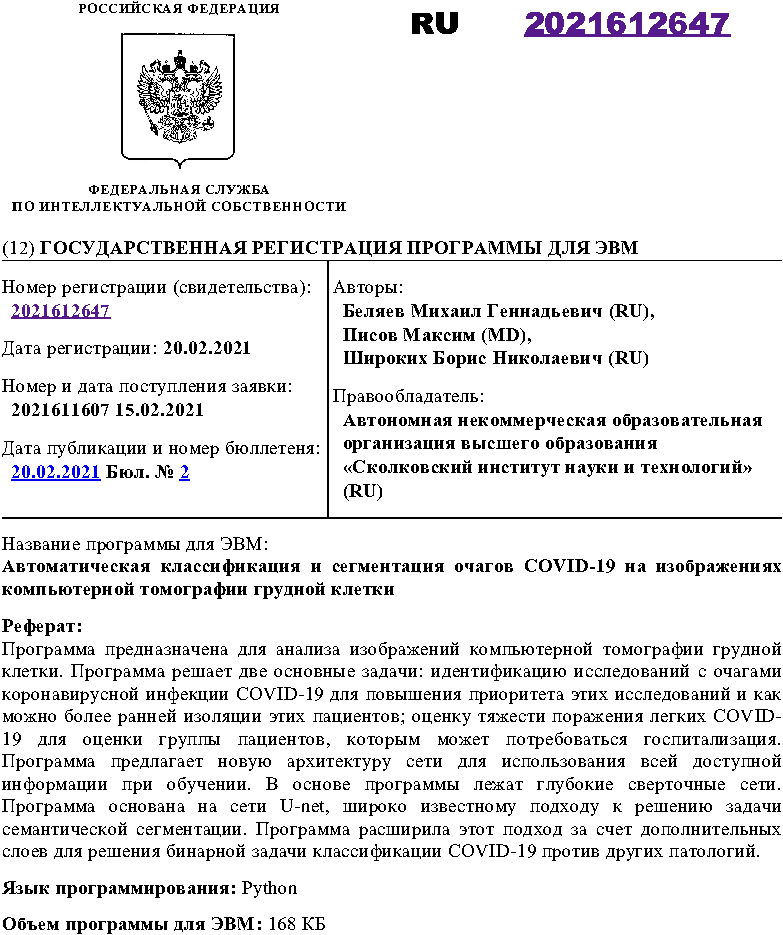
\includegraphics[width=0.95\textwidth]{Dissertation/Figures/6_appendix/output_crop.pdf}
\end{center}

        % Приложения

\setcounter{totalappendix}{\value{chapter}} % Подсчёт количества приложений

\end{document}
